\documentclass[twoside]{book}

% Packages required by doxygen
\usepackage{fixltx2e}
\usepackage{calc}
\usepackage{doxygen}
\usepackage[export]{adjustbox} % also loads graphicx
\usepackage{graphicx}
\usepackage[utf8]{inputenc}
\usepackage{makeidx}
\usepackage{multicol}
\usepackage{multirow}
\PassOptionsToPackage{warn}{textcomp}
\usepackage{textcomp}
\usepackage[nointegrals]{wasysym}
\usepackage[table]{xcolor}

% Font selection
\usepackage[T1]{fontenc}
\usepackage[scaled=.90]{helvet}
\usepackage{courier}
\usepackage{amssymb}
\usepackage{sectsty}
\renewcommand{\familydefault}{\sfdefault}
\allsectionsfont{%
  \fontseries{bc}\selectfont%
  \color{darkgray}%
}
\renewcommand{\DoxyLabelFont}{%
  \fontseries{bc}\selectfont%
  \color{darkgray}%
}
\newcommand{\+}{\discretionary{\mbox{\scriptsize$\hookleftarrow$}}{}{}}

% Page & text layout
\usepackage{geometry}
\geometry{%
  a4paper,%
  top=2.5cm,%
  bottom=2.5cm,%
  left=2.5cm,%
  right=2.5cm%
}
\tolerance=750
\hfuzz=15pt
\hbadness=750
\setlength{\emergencystretch}{15pt}
\setlength{\parindent}{0cm}
\setlength{\parskip}{3ex plus 2ex minus 2ex}
\makeatletter
\renewcommand{\paragraph}{%
  \@startsection{paragraph}{4}{0ex}{-1.0ex}{1.0ex}{%
    \normalfont\normalsize\bfseries\SS@parafont%
  }%
}
\renewcommand{\subparagraph}{%
  \@startsection{subparagraph}{5}{0ex}{-1.0ex}{1.0ex}{%
    \normalfont\normalsize\bfseries\SS@subparafont%
  }%
}
\makeatother

% Headers & footers
\usepackage{fancyhdr}
\pagestyle{fancyplain}
\fancyhead[LE]{\fancyplain{}{\bfseries\thepage}}
\fancyhead[CE]{\fancyplain{}{}}
\fancyhead[RE]{\fancyplain{}{\bfseries\leftmark}}
\fancyhead[LO]{\fancyplain{}{\bfseries\rightmark}}
\fancyhead[CO]{\fancyplain{}{}}
\fancyhead[RO]{\fancyplain{}{\bfseries\thepage}}
\fancyfoot[LE]{\fancyplain{}{}}
\fancyfoot[CE]{\fancyplain{}{}}
\fancyfoot[RE]{\fancyplain{}{\bfseries\scriptsize Generated by Doxygen }}
\fancyfoot[LO]{\fancyplain{}{\bfseries\scriptsize Generated by Doxygen }}
\fancyfoot[CO]{\fancyplain{}{}}
\fancyfoot[RO]{\fancyplain{}{}}
\renewcommand{\footrulewidth}{0.4pt}
\renewcommand{\chaptermark}[1]{%
  \markboth{#1}{}%
}
\renewcommand{\sectionmark}[1]{%
  \markright{\thesection\ #1}%
}

% Indices & bibliography
\usepackage{natbib}
\usepackage[titles]{tocloft}
\setcounter{tocdepth}{3}
\setcounter{secnumdepth}{5}
\makeindex

% Hyperlinks (required, but should be loaded last)
\usepackage{ifpdf}
\ifpdf
  \usepackage[pdftex,pagebackref=true]{hyperref}
\else
  \usepackage[ps2pdf,pagebackref=true]{hyperref}
\fi
\hypersetup{%
  colorlinks=true,%
  linkcolor=blue,%
  citecolor=blue,%
  unicode%
}

% Custom commands
\newcommand{\clearemptydoublepage}{%
  \newpage{\pagestyle{empty}\cleardoublepage}%
}

\usepackage{caption}
\captionsetup{labelsep=space,justification=centering,font={bf},singlelinecheck=off,skip=4pt,position=top}

%===== C O N T E N T S =====

\begin{document}

% Titlepage & ToC
\hypersetup{pageanchor=false,
             bookmarksnumbered=true,
             pdfencoding=unicode
            }
\pagenumbering{alph}
\begin{titlepage}
\vspace*{7cm}
\begin{center}%
{\Large dialog }\\
\vspace*{1cm}
{\large Generated by Doxygen 1.8.13}\\
\end{center}
\end{titlepage}
\clearemptydoublepage
\pagenumbering{roman}
\tableofcontents
\clearemptydoublepage
\pagenumbering{arabic}
\hypersetup{pageanchor=true}

%--- Begin generated contents ---
\chapter{Hierarchical Index}
\section{Class Hierarchy}
This inheritance list is sorted roughly, but not completely, alphabetically\+:\begin{DoxyCompactList}
\item \contentsline{section}{dialog\+:\+:aggop\+\_\+utils}{\pageref{classdialog_1_1aggop__utils}}{}
\item \contentsline{section}{dialog\+:\+:aggregate}{\pageref{classdialog_1_1aggregate}}{}
\item \contentsline{section}{dialog\+:\+:aggregate\+\_\+list}{\pageref{classdialog_1_1aggregate__list}}{}
\item \contentsline{section}{dialog\+:\+:aggregate\+\_\+node}{\pageref{structdialog_1_1aggregate__node}}{}
\item \contentsline{section}{dialog\+:\+:aggregator}{\pageref{structdialog_1_1aggregator}}{}
\item \contentsline{section}{dialog\+:\+:monitor\+:\+:alert}{\pageref{structdialog_1_1monitor_1_1alert}}{}
\item \contentsline{section}{dialog\+:\+:monitor\+:\+:alert\+\_\+index}{\pageref{classdialog_1_1monitor_1_1alert__index}}{}
\item \contentsline{section}{dialog\+:\+:bitmap}{\pageref{classdialog_1_1bitmap}}{}
\begin{DoxyCompactList}
\item \contentsline{section}{dialog\+:\+:bitmap\+\_\+array\+\_\+base$<$ pos\+\_\+type $>$}{\pageref{classdialog_1_1bitmap__array__base}}{}
\item \contentsline{section}{dialog\+:\+:bitmap\+\_\+array\+\_\+base$<$ T $>$}{\pageref{classdialog_1_1bitmap__array__base}}{}
\begin{DoxyCompactList}
\item \contentsline{section}{dialog\+:\+:signed\+\_\+bitmap\+\_\+array$<$ T $>$}{\pageref{classdialog_1_1signed__bitmap__array}}{}
\item \contentsline{section}{dialog\+:\+:unsigned\+\_\+bitmap\+\_\+array$<$ T $>$}{\pageref{classdialog_1_1unsigned__bitmap__array}}{}
\end{DoxyCompactList}
\item \contentsline{section}{dialog\+:\+:unsized\+\_\+bitmap\+\_\+array$<$ T $>$}{\pageref{classdialog_1_1unsized__bitmap__array}}{}
\item \contentsline{section}{dialog\+:\+:unsized\+\_\+bitmap\+\_\+array$<$ pos\+\_\+type $>$}{\pageref{classdialog_1_1unsized__bitmap__array}}{}
\end{DoxyCompactList}
\item \contentsline{section}{dialog\+:\+:bitmap\+\_\+array\+\_\+iterator$<$ bitmap\+\_\+array\+\_\+impl $>$}{\pageref{classdialog_1_1bitmap__array__iterator}}{}
\item \contentsline{section}{dialog\+:\+:byte\+\_\+string}{\pageref{classdialog_1_1byte__string}}{}
\item \contentsline{section}{dialog\+:\+:column\+\_\+snapshot}{\pageref{structdialog_1_1column__snapshot}}{}
\item \contentsline{section}{dialog\+:\+:column\+\_\+t}{\pageref{classdialog_1_1column__t}}{}
\item \contentsline{section}{dialog\+:\+:compiled\+\_\+minterm}{\pageref{structdialog_1_1compiled__minterm}}{}
\item \contentsline{section}{dialog\+:\+:compiled\+\_\+predicate}{\pageref{structdialog_1_1compiled__predicate}}{}
\item \contentsline{section}{dialog\+:\+:configuration\+\_\+params}{\pageref{classdialog_1_1configuration__params}}{}
\item \contentsline{section}{dialog\+:\+:const\+\_\+bitmap\+\_\+array\+\_\+iterator$<$ bitmap\+\_\+array\+\_\+impl $>$}{\pageref{classdialog_1_1const__bitmap__array__iterator}}{}
\item \contentsline{section}{dialog\+:\+:constants}{\pageref{classdialog_1_1constants}}{}
\item \contentsline{section}{dialog\+:\+:data}{\pageref{structdialog_1_1data}}{}
\item \contentsline{section}{dialog\+:\+:data\+\_\+type}{\pageref{structdialog_1_1data__type}}{}
\item \contentsline{section}{dialog\+:\+:delta\+\_\+encoded\+\_\+array$<$ T, sampling\+\_\+rate $>$}{\pageref{classdialog_1_1delta__encoded__array}}{}
\begin{DoxyCompactList}
\item \contentsline{section}{dialog\+:\+:elias\+\_\+gamma\+\_\+encoded\+\_\+array$<$ T, sampling\+\_\+rate $>$}{\pageref{classdialog_1_1elias__gamma__encoded__array}}{}
\end{DoxyCompactList}
\item \contentsline{section}{dialog\+:\+:dialog\+\_\+store}{\pageref{classdialog_1_1dialog__store}}{}
\item \contentsline{section}{dialog\+:\+:dialog\+\_\+table}{\pageref{classdialog_1_1dialog__table}}{}
\item \contentsline{section}{dialog\+:\+:storage\+:\+:durable}{\pageref{structdialog_1_1storage_1_1durable}}{}
\item \contentsline{section}{dialog\+:\+:storage\+:\+:durable\+\_\+relaxed}{\pageref{structdialog_1_1storage_1_1durable__relaxed}}{}
\item \contentsline{section}{dialog\+:\+:index\+:\+:empty\+\_\+stats}{\pageref{structdialog_1_1index_1_1empty__stats}}{}
\item \contentsline{section}{dialog\+:\+:expression\+\_\+compiler}{\pageref{classdialog_1_1expression__compiler}}{}
\item \contentsline{section}{dialog\+:\+:expression\+\_\+lex\+\_\+token}{\pageref{structdialog_1_1expression__lex__token}}{}
\item \contentsline{section}{dialog\+:\+:expression\+\_\+lexer}{\pageref{classdialog_1_1expression__lexer}}{}
\item \contentsline{section}{dialog\+:\+:expression\+\_\+parser}{\pageref{classdialog_1_1expression__parser}}{}
\item \contentsline{section}{dialog\+:\+:expression\+\_\+t}{\pageref{structdialog_1_1expression__t}}{}
\begin{DoxyCompactList}
\item \contentsline{section}{dialog\+:\+:conjunction\+\_\+t}{\pageref{structdialog_1_1conjunction__t}}{}
\item \contentsline{section}{dialog\+:\+:disjunction\+\_\+t}{\pageref{structdialog_1_1disjunction__t}}{}
\item \contentsline{section}{dialog\+:\+:negation}{\pageref{structdialog_1_1negation}}{}
\item \contentsline{section}{dialog\+:\+:predicate\+\_\+t}{\pageref{structdialog_1_1predicate__t}}{}
\end{DoxyCompactList}
\item \contentsline{section}{dialog\+:\+:expression\+\_\+utils}{\pageref{classdialog_1_1expression__utils}}{}
\item \contentsline{section}{dialog\+:\+:field\+\_\+t}{\pageref{structdialog_1_1field__t}}{}
\item \contentsline{section}{dialog\+:\+:monitor\+:\+:filter}{\pageref{classdialog_1_1monitor_1_1filter}}{}
\item \contentsline{section}{dialog\+:\+:filter\+\_\+info}{\pageref{structdialog_1_1filter__info}}{}
\item \contentsline{section}{dialog\+:\+:filtered\+\_\+record\+\_\+stream$<$ rstream\+\_\+t $>$}{\pageref{classdialog_1_1filtered__record__stream}}{}
\item \contentsline{section}{flattened\+\_\+container$<$ container\+\_\+t $>$}{\pageref{classflattened__container}}{}
\item \contentsline{section}{flattened\+\_\+iterator$<$ outer\+\_\+iterator $>$}{\pageref{classflattened__iterator}}{}
\item \contentsline{section}{dialog\+:\+:immutable\+\_\+byte\+\_\+string}{\pageref{classdialog_1_1immutable__byte__string}}{}
\item \contentsline{section}{dialog\+:\+:immutable\+\_\+value}{\pageref{classdialog_1_1immutable__value}}{}
\begin{DoxyCompactList}
\item \contentsline{section}{dialog\+:\+:mutable\+\_\+value}{\pageref{classdialog_1_1mutable__value}}{}
\end{DoxyCompactList}
\item \contentsline{section}{dialog\+:\+:storage\+:\+:in\+\_\+memory}{\pageref{structdialog_1_1storage_1_1in__memory}}{}
\item \contentsline{section}{dialog\+:\+:index\+\_\+filter}{\pageref{classdialog_1_1index__filter}}{}
\item \contentsline{section}{dialog\+:\+:index\+\_\+info}{\pageref{structdialog_1_1index__info}}{}
\item \contentsline{section}{dialog\+:\+:index\+\_\+state\+\_\+t}{\pageref{structdialog_1_1index__state__t}}{}
\item \contentsline{section}{dialog\+:\+:index\+:\+:indexlet$<$ T, S\+I\+ZE $>$}{\pageref{classdialog_1_1index_1_1indexlet}}{}
\item \contentsline{section}{dialog\+:\+:index\+:\+:indexlet$<$ child\+\_\+type, K $>$}{\pageref{classdialog_1_1index_1_1indexlet}}{}
\item \contentsline{section}{dialog\+:\+:index\+:\+:indexlet$<$ T, K $>$}{\pageref{classdialog_1_1index_1_1indexlet}}{}
\item iterator\begin{DoxyCompactList}
\item \contentsline{section}{dialog\+:\+:index\+:\+:rt\+\_\+reflog\+\_\+it$<$ reflog $>$}{\pageref{classdialog_1_1index_1_1rt__reflog__it}}{}
\item \contentsline{section}{dialog\+:\+:monolog\+:\+:monolog\+\_\+iterator$<$ monolog\+\_\+impl $>$}{\pageref{classdialog_1_1monolog_1_1monolog__iterator}}{}
\end{DoxyCompactList}
\item \contentsline{section}{dialog\+:\+:string\+\_\+map$<$ V $>$\+:\+:map\+\_\+entry}{\pageref{structdialog_1_1string__map_1_1map__entry}}{}
\item \contentsline{section}{dialog\+:\+:marked\+\_\+ptr$<$ T $>$}{\pageref{structdialog_1_1marked__ptr}}{}
\item \contentsline{section}{dialog\+:\+:marked\+\_\+ptr$<$ node\+\_\+t $>$}{\pageref{structdialog_1_1marked__ptr}}{}
\item \contentsline{section}{dialog\+:\+:metadata\+\_\+reader}{\pageref{classdialog_1_1metadata__reader}}{}
\item \contentsline{section}{dialog\+:\+:metadata\+\_\+writer}{\pageref{classdialog_1_1metadata__writer}}{}
\item \contentsline{section}{dialog\+:\+:minterm\+\_\+plan}{\pageref{classdialog_1_1minterm__plan}}{}
\item \contentsline{section}{dialog\+:\+:monolog\+:\+:monolog\+\_\+block$<$ T, B\+U\+F\+F\+E\+R\+\_\+\+S\+I\+ZE $>$}{\pageref{classdialog_1_1monolog_1_1monolog__block}}{}
\item \contentsline{section}{dialog\+:\+:monolog\+:\+:monolog\+\_\+exp2\+\_\+base$<$ T, N\+B\+U\+C\+K\+E\+TS $>$}{\pageref{classdialog_1_1monolog_1_1monolog__exp2__base}}{}
\begin{DoxyCompactList}
\item \contentsline{section}{dialog\+:\+:monolog\+:\+:monolog\+\_\+exp2$<$ T, N\+B\+U\+C\+K\+E\+TS $>$}{\pageref{classdialog_1_1monolog_1_1monolog__exp2}}{}
\end{DoxyCompactList}
\item \contentsline{section}{dialog\+:\+:monolog\+:\+:monolog\+\_\+exp2\+\_\+linear\+\_\+base$<$ T, N\+C\+O\+N\+T\+A\+I\+N\+E\+RS, B\+U\+C\+K\+E\+T\+\_\+\+S\+I\+ZE $>$}{\pageref{classdialog_1_1monolog_1_1monolog__exp2__linear__base}}{}
\begin{DoxyCompactList}
\item \contentsline{section}{dialog\+:\+:monolog\+:\+:monolog\+\_\+exp2\+\_\+linear$<$ T, N\+C\+O\+N\+T\+A\+I\+N\+E\+RS, B\+U\+C\+K\+E\+T\+\_\+\+S\+I\+ZE $>$}{\pageref{classdialog_1_1monolog_1_1monolog__exp2__linear}}{}
\begin{DoxyCompactList}
\item \contentsline{section}{dialog\+:\+:aggregated\+\_\+reflog}{\pageref{classdialog_1_1aggregated__reflog}}{}
\end{DoxyCompactList}
\end{DoxyCompactList}
\item \contentsline{section}{dialog\+:\+:monolog\+:\+:monolog\+\_\+exp2\+\_\+linear\+\_\+base$<$ dialog\+:\+:dialog\+\_\+table $\ast$, 32, 1024 $>$}{\pageref{classdialog_1_1monolog_1_1monolog__exp2__linear__base}}{}
\begin{DoxyCompactList}
\item \contentsline{section}{dialog\+:\+:monolog\+:\+:monolog\+\_\+exp2\+\_\+linear$<$ dialog\+:\+:dialog\+\_\+table $\ast$$>$}{\pageref{classdialog_1_1monolog_1_1monolog__exp2__linear}}{}
\end{DoxyCompactList}
\item \contentsline{section}{dialog\+:\+:monolog\+:\+:monolog\+\_\+exp2\+\_\+linear\+\_\+base$<$ dialog\+:\+:string\+\_\+map\+:\+:map\+\_\+entry, 32, 1024 $>$}{\pageref{classdialog_1_1monolog_1_1monolog__exp2__linear__base}}{}
\begin{DoxyCompactList}
\item \contentsline{section}{dialog\+:\+:monolog\+:\+:monolog\+\_\+exp2\+\_\+linear$<$ dialog\+:\+:string\+\_\+map\+:\+:map\+\_\+entry $>$}{\pageref{classdialog_1_1monolog_1_1monolog__exp2__linear}}{}
\end{DoxyCompactList}
\item \contentsline{section}{dialog\+:\+:monolog\+:\+:monolog\+\_\+exp2\+\_\+linear\+\_\+base$<$ index\+:\+:radix\+\_\+index $\ast$, 32, 1024 $>$}{\pageref{classdialog_1_1monolog_1_1monolog__exp2__linear__base}}{}
\begin{DoxyCompactList}
\item \contentsline{section}{dialog\+:\+:monolog\+:\+:monolog\+\_\+exp2\+\_\+linear$<$ index\+:\+:radix\+\_\+index $\ast$ $>$}{\pageref{classdialog_1_1monolog_1_1monolog__exp2__linear}}{}
\end{DoxyCompactList}
\item \contentsline{section}{dialog\+:\+:monolog\+:\+:monolog\+\_\+exp2\+\_\+linear\+\_\+base$<$ monitor\+:\+:filter $\ast$, 32, 1024 $>$}{\pageref{classdialog_1_1monolog_1_1monolog__exp2__linear__base}}{}
\begin{DoxyCompactList}
\item \contentsline{section}{dialog\+:\+:monolog\+:\+:monolog\+\_\+exp2\+\_\+linear$<$ monitor\+:\+:filter $\ast$ $>$}{\pageref{classdialog_1_1monolog_1_1monolog__exp2__linear}}{}
\end{DoxyCompactList}
\item \contentsline{section}{dialog\+:\+:monolog\+:\+:monolog\+\_\+exp2\+\_\+linear\+\_\+base$<$ monitor\+:\+:trigger $\ast$, 32, 1024 $>$}{\pageref{classdialog_1_1monolog_1_1monolog__exp2__linear__base}}{}
\begin{DoxyCompactList}
\item \contentsline{section}{dialog\+:\+:monolog\+:\+:monolog\+\_\+exp2\+\_\+linear$<$ monitor\+:\+:trigger $\ast$ $>$}{\pageref{classdialog_1_1monolog_1_1monolog__exp2__linear}}{}
\end{DoxyCompactList}
\item \contentsline{section}{dialog\+:\+:monolog\+:\+:monolog\+\_\+linear\+\_\+base$<$ T, M\+A\+X\+\_\+\+B\+L\+O\+C\+KS, B\+L\+O\+C\+K\+\_\+\+S\+I\+ZE, B\+U\+F\+F\+E\+R\+\_\+\+S\+I\+ZE $>$}{\pageref{classdialog_1_1monolog_1_1monolog__linear__base}}{}
\begin{DoxyCompactList}
\item \contentsline{section}{dialog\+:\+:monolog\+:\+:monolog\+\_\+linear$<$ T, M\+A\+X\+\_\+\+B\+L\+O\+C\+KS, B\+L\+O\+C\+K\+\_\+\+S\+I\+ZE, B\+U\+F\+F\+E\+R\+\_\+\+S\+I\+ZE $>$}{\pageref{classdialog_1_1monolog_1_1monolog__linear}}{}
\end{DoxyCompactList}
\item \contentsline{section}{dialog\+:\+:numeric}{\pageref{classdialog_1_1numeric}}{}
\item \contentsline{section}{dialog\+:\+:optional$<$ T $>$}{\pageref{classdialog_1_1optional}}{}
\item \contentsline{section}{dialog\+:\+:parsed\+\_\+trigger}{\pageref{structdialog_1_1parsed__trigger}}{}
\item \contentsline{section}{periodic\+\_\+task}{\pageref{classperiodic__task}}{}
\item \contentsline{section}{dialog\+:\+:query\+\_\+planner}{\pageref{classdialog_1_1query__planner}}{}
\item \contentsline{section}{dialog\+:\+:index\+:\+:radix\+\_\+tree$<$ reflog $>$}{\pageref{classdialog_1_1index_1_1radix__tree}}{}
\item \contentsline{section}{dialog\+:\+:index\+:\+:radix\+\_\+tree$<$ aggregated\+\_\+reflog $>$}{\pageref{classdialog_1_1index_1_1radix__tree}}{}
\item \contentsline{section}{dialog\+:\+:index\+:\+:radix\+\_\+tree$<$ alert\+\_\+log $>$}{\pageref{classdialog_1_1index_1_1radix__tree}}{}
\item \contentsline{section}{dialog\+:\+:index\+:\+:radix\+\_\+tree\+\_\+node$<$ reflog $>$}{\pageref{structdialog_1_1index_1_1radix__tree__node}}{}
\item \contentsline{section}{dialog\+:\+:read\+\_\+tail}{\pageref{classdialog_1_1read__tail}}{}
\item \contentsline{section}{dialog\+:\+:record\+\_\+batch}{\pageref{structdialog_1_1record__batch}}{}
\item \contentsline{section}{dialog\+:\+:record\+\_\+batch\+\_\+builder}{\pageref{classdialog_1_1record__batch__builder}}{}
\item \contentsline{section}{dialog\+:\+:record\+\_\+block}{\pageref{structdialog_1_1record__block}}{}
\item \contentsline{section}{dialog\+:\+:record\+\_\+stream$<$ offset\+\_\+container $>$}{\pageref{classdialog_1_1record__stream}}{}
\item \contentsline{section}{dialog\+:\+:record\+\_\+t}{\pageref{structdialog_1_1record__t}}{}
\item \contentsline{section}{dialog\+:\+:relop\+\_\+utils}{\pageref{classdialog_1_1relop__utils}}{}
\item \contentsline{section}{dialog\+:\+:index\+:\+:rt\+\_\+reflog\+\_\+range\+\_\+result$<$ reflog $>$}{\pageref{classdialog_1_1index_1_1rt__reflog__range__result}}{}
\item \contentsline{section}{dialog\+:\+:schema\+\_\+builder}{\pageref{classdialog_1_1schema__builder}}{}
\item \contentsline{section}{dialog\+:\+:schema\+\_\+snapshot}{\pageref{classdialog_1_1schema__snapshot}}{}
\item \contentsline{section}{dialog\+:\+:schema\+\_\+t}{\pageref{classdialog_1_1schema__t}}{}
\item \contentsline{section}{dialog\+:\+:searchable\+\_\+list$<$ K, V $>$}{\pageref{structdialog_1_1searchable__list}}{}
\item \contentsline{section}{dialog\+:\+:searchable\+\_\+list\+\_\+node$<$ K, V $>$}{\pageref{structdialog_1_1searchable__list__node}}{}
\item set\begin{DoxyCompactList}
\item \contentsline{section}{dialog\+:\+:compiled\+\_\+expression}{\pageref{structdialog_1_1compiled__expression}}{}
\end{DoxyCompactList}
\item \contentsline{section}{dialog\+:\+:storage\+:\+:storage\+\_\+mode}{\pageref{structdialog_1_1storage_1_1storage__mode}}{}
\item \contentsline{section}{dialog\+:\+:string\+\_\+map$<$ V $>$\+:\+:string\+\_\+hash}{\pageref{structdialog_1_1string__map_1_1string__hash}}{}
\item \contentsline{section}{dialog\+:\+:string\+\_\+map$<$ V $>$}{\pageref{classdialog_1_1string__map}}{}
\item \contentsline{section}{dialog\+:\+:string\+\_\+map$<$ filter\+\_\+id\+\_\+t $>$}{\pageref{classdialog_1_1string__map}}{}
\item \contentsline{section}{dialog\+:\+:string\+\_\+map$<$ size\+\_\+t $>$}{\pageref{classdialog_1_1string__map}}{}
\item \contentsline{section}{dialog\+:\+:string\+\_\+map$<$ trigger\+\_\+id\+\_\+t $>$}{\pageref{classdialog_1_1string__map}}{}
\item \contentsline{section}{task\+\_\+pool}{\pageref{classtask__pool}}{}
\item \contentsline{section}{task\+\_\+queue}{\pageref{classtask__queue}}{}
\item \contentsline{section}{task\+\_\+type}{\pageref{structtask__type}}{}
\item \contentsline{section}{task\+\_\+worker}{\pageref{classtask__worker}}{}
\item \contentsline{section}{dialog\+:\+:thread\+\_\+info}{\pageref{structdialog_1_1thread__info}}{}
\item \contentsline{section}{dialog\+:\+:thread\+\_\+manager}{\pageref{classdialog_1_1thread__manager}}{}
\item \contentsline{section}{dialog\+:\+:index\+:\+:tiered\+\_\+index$<$ T, K, D, stats $>$}{\pageref{classdialog_1_1index_1_1tiered__index}}{}
\item \contentsline{section}{dialog\+:\+:index\+:\+:tiered\+\_\+index$<$ T, K, 1, stats $>$}{\pageref{classdialog_1_1index_1_1tiered__index_3_01_t_00_01_k_00_011_00_01stats_01_4}}{}
\item \contentsline{section}{dialog\+:\+:monitor\+:\+:trigger}{\pageref{structdialog_1_1monitor_1_1trigger}}{}
\item \contentsline{section}{dialog\+:\+:trigger\+\_\+info}{\pageref{structdialog_1_1trigger__info}}{}
\item \contentsline{section}{dialog\+:\+:trigger\+\_\+lex\+\_\+token}{\pageref{structdialog_1_1trigger__lex__token}}{}
\item \contentsline{section}{dialog\+:\+:trigger\+\_\+lexer}{\pageref{classdialog_1_1trigger__lexer}}{}
\item \contentsline{section}{dialog\+:\+:trigger\+\_\+parser}{\pageref{classdialog_1_1trigger__parser}}{}
\item \contentsline{section}{dialog\+:\+:union\+\_\+record\+\_\+stream$<$ rstream\+\_\+t $>$}{\pageref{classdialog_1_1union__record__stream}}{}
\item \contentsline{section}{dialog\+:\+:value\+\_\+reference$<$ bitmap\+\_\+array\+\_\+impl $>$}{\pageref{classdialog_1_1value__reference}}{}
\item vector\begin{DoxyCompactList}
\item \contentsline{section}{dialog\+:\+:query\+\_\+plan}{\pageref{classdialog_1_1query__plan}}{}
\end{DoxyCompactList}
\end{DoxyCompactList}

\chapter{Class Index}
\section{Class List}
Here are the classes, structs, unions and interfaces with brief descriptions\+:\begin{DoxyCompactList}
\item\contentsline{section}{\hyperlink{classdialog_1_1aggop__utils}{dialog\+::aggop\+\_\+utils} }{\pageref{classdialog_1_1aggop__utils}}{}
\item\contentsline{section}{\hyperlink{classdialog_1_1aggregate}{dialog\+::aggregate} }{\pageref{classdialog_1_1aggregate}}{}
\item\contentsline{section}{\hyperlink{classdialog_1_1aggregate__list}{dialog\+::aggregate\+\_\+list} }{\pageref{classdialog_1_1aggregate__list}}{}
\item\contentsline{section}{\hyperlink{structdialog_1_1aggregate__node}{dialog\+::aggregate\+\_\+node} }{\pageref{structdialog_1_1aggregate__node}}{}
\item\contentsline{section}{\hyperlink{classdialog_1_1aggregated__reflog}{dialog\+::aggregated\+\_\+reflog} }{\pageref{classdialog_1_1aggregated__reflog}}{}
\item\contentsline{section}{\hyperlink{structdialog_1_1aggregator}{dialog\+::aggregator} }{\pageref{structdialog_1_1aggregator}}{}
\item\contentsline{section}{\hyperlink{structdialog_1_1monitor_1_1alert}{dialog\+::monitor\+::alert} }{\pageref{structdialog_1_1monitor_1_1alert}}{}
\item\contentsline{section}{\hyperlink{classdialog_1_1monitor_1_1alert__index}{dialog\+::monitor\+::alert\+\_\+index} }{\pageref{classdialog_1_1monitor_1_1alert__index}}{}
\item\contentsline{section}{\hyperlink{classdialog_1_1bitmap}{dialog\+::bitmap} }{\pageref{classdialog_1_1bitmap}}{}
\item\contentsline{section}{\hyperlink{classdialog_1_1bitmap__array__base}{dialog\+::bitmap\+\_\+array\+\_\+base$<$ T $>$} }{\pageref{classdialog_1_1bitmap__array__base}}{}
\item\contentsline{section}{\hyperlink{classdialog_1_1bitmap__array__iterator}{dialog\+::bitmap\+\_\+array\+\_\+iterator$<$ bitmap\+\_\+array\+\_\+impl $>$} }{\pageref{classdialog_1_1bitmap__array__iterator}}{}
\item\contentsline{section}{\hyperlink{classdialog_1_1byte__string}{dialog\+::byte\+\_\+string} }{\pageref{classdialog_1_1byte__string}}{}
\item\contentsline{section}{\hyperlink{structdialog_1_1column__snapshot}{dialog\+::column\+\_\+snapshot} }{\pageref{structdialog_1_1column__snapshot}}{}
\item\contentsline{section}{\hyperlink{classdialog_1_1column__t}{dialog\+::column\+\_\+t} }{\pageref{classdialog_1_1column__t}}{}
\item\contentsline{section}{\hyperlink{structdialog_1_1compiled__expression}{dialog\+::compiled\+\_\+expression} }{\pageref{structdialog_1_1compiled__expression}}{}
\item\contentsline{section}{\hyperlink{structdialog_1_1compiled__minterm}{dialog\+::compiled\+\_\+minterm} }{\pageref{structdialog_1_1compiled__minterm}}{}
\item\contentsline{section}{\hyperlink{structdialog_1_1compiled__predicate}{dialog\+::compiled\+\_\+predicate} }{\pageref{structdialog_1_1compiled__predicate}}{}
\item\contentsline{section}{\hyperlink{classdialog_1_1configuration__params}{dialog\+::configuration\+\_\+params} }{\pageref{classdialog_1_1configuration__params}}{}
\item\contentsline{section}{\hyperlink{structdialog_1_1conjunction__t}{dialog\+::conjunction\+\_\+t} }{\pageref{structdialog_1_1conjunction__t}}{}
\item\contentsline{section}{\hyperlink{classdialog_1_1const__bitmap__array__iterator}{dialog\+::const\+\_\+bitmap\+\_\+array\+\_\+iterator$<$ bitmap\+\_\+array\+\_\+impl $>$} }{\pageref{classdialog_1_1const__bitmap__array__iterator}}{}
\item\contentsline{section}{\hyperlink{classdialog_1_1constants}{dialog\+::constants} }{\pageref{classdialog_1_1constants}}{}
\item\contentsline{section}{\hyperlink{structdialog_1_1data}{dialog\+::data} }{\pageref{structdialog_1_1data}}{}
\item\contentsline{section}{\hyperlink{structdialog_1_1data__type}{dialog\+::data\+\_\+type} }{\pageref{structdialog_1_1data__type}}{}
\item\contentsline{section}{\hyperlink{classdialog_1_1delta__encoded__array}{dialog\+::delta\+\_\+encoded\+\_\+array$<$ T, sampling\+\_\+rate $>$} }{\pageref{classdialog_1_1delta__encoded__array}}{}
\item\contentsline{section}{\hyperlink{classdialog_1_1dialog__store}{dialog\+::dialog\+\_\+store} }{\pageref{classdialog_1_1dialog__store}}{}
\item\contentsline{section}{\hyperlink{classdialog_1_1dialog__table}{dialog\+::dialog\+\_\+table} }{\pageref{classdialog_1_1dialog__table}}{}
\item\contentsline{section}{\hyperlink{structdialog_1_1disjunction__t}{dialog\+::disjunction\+\_\+t} }{\pageref{structdialog_1_1disjunction__t}}{}
\item\contentsline{section}{\hyperlink{structdialog_1_1storage_1_1durable}{dialog\+::storage\+::durable} }{\pageref{structdialog_1_1storage_1_1durable}}{}
\item\contentsline{section}{\hyperlink{structdialog_1_1storage_1_1durable__relaxed}{dialog\+::storage\+::durable\+\_\+relaxed} }{\pageref{structdialog_1_1storage_1_1durable__relaxed}}{}
\item\contentsline{section}{\hyperlink{classdialog_1_1elias__gamma__encoded__array}{dialog\+::elias\+\_\+gamma\+\_\+encoded\+\_\+array$<$ T, sampling\+\_\+rate $>$} }{\pageref{classdialog_1_1elias__gamma__encoded__array}}{}
\item\contentsline{section}{\hyperlink{structdialog_1_1index_1_1empty__stats}{dialog\+::index\+::empty\+\_\+stats} }{\pageref{structdialog_1_1index_1_1empty__stats}}{}
\item\contentsline{section}{\hyperlink{classdialog_1_1expression__compiler}{dialog\+::expression\+\_\+compiler} }{\pageref{classdialog_1_1expression__compiler}}{}
\item\contentsline{section}{\hyperlink{structdialog_1_1expression__lex__token}{dialog\+::expression\+\_\+lex\+\_\+token} }{\pageref{structdialog_1_1expression__lex__token}}{}
\item\contentsline{section}{\hyperlink{classdialog_1_1expression__lexer}{dialog\+::expression\+\_\+lexer} }{\pageref{classdialog_1_1expression__lexer}}{}
\item\contentsline{section}{\hyperlink{classdialog_1_1expression__parser}{dialog\+::expression\+\_\+parser} }{\pageref{classdialog_1_1expression__parser}}{}
\item\contentsline{section}{\hyperlink{structdialog_1_1expression__t}{dialog\+::expression\+\_\+t} }{\pageref{structdialog_1_1expression__t}}{}
\item\contentsline{section}{\hyperlink{classdialog_1_1expression__utils}{dialog\+::expression\+\_\+utils} }{\pageref{classdialog_1_1expression__utils}}{}
\item\contentsline{section}{\hyperlink{structdialog_1_1field__t}{dialog\+::field\+\_\+t} }{\pageref{structdialog_1_1field__t}}{}
\item\contentsline{section}{\hyperlink{classdialog_1_1monitor_1_1filter}{dialog\+::monitor\+::filter} }{\pageref{classdialog_1_1monitor_1_1filter}}{}
\item\contentsline{section}{\hyperlink{structdialog_1_1filter__info}{dialog\+::filter\+\_\+info} }{\pageref{structdialog_1_1filter__info}}{}
\item\contentsline{section}{\hyperlink{classdialog_1_1filtered__record__stream}{dialog\+::filtered\+\_\+record\+\_\+stream$<$ rstream\+\_\+t $>$} }{\pageref{classdialog_1_1filtered__record__stream}}{}
\item\contentsline{section}{\hyperlink{classflattened__container}{flattened\+\_\+container$<$ container\+\_\+t $>$} }{\pageref{classflattened__container}}{}
\item\contentsline{section}{\hyperlink{classflattened__iterator}{flattened\+\_\+iterator$<$ outer\+\_\+iterator $>$} }{\pageref{classflattened__iterator}}{}
\item\contentsline{section}{\hyperlink{classdialog_1_1immutable__byte__string}{dialog\+::immutable\+\_\+byte\+\_\+string} }{\pageref{classdialog_1_1immutable__byte__string}}{}
\item\contentsline{section}{\hyperlink{classdialog_1_1immutable__value}{dialog\+::immutable\+\_\+value} }{\pageref{classdialog_1_1immutable__value}}{}
\item\contentsline{section}{\hyperlink{structdialog_1_1storage_1_1in__memory}{dialog\+::storage\+::in\+\_\+memory} }{\pageref{structdialog_1_1storage_1_1in__memory}}{}
\item\contentsline{section}{\hyperlink{classdialog_1_1index__filter}{dialog\+::index\+\_\+filter} }{\pageref{classdialog_1_1index__filter}}{}
\item\contentsline{section}{\hyperlink{structdialog_1_1index__info}{dialog\+::index\+\_\+info} }{\pageref{structdialog_1_1index__info}}{}
\item\contentsline{section}{\hyperlink{structdialog_1_1index__state__t}{dialog\+::index\+\_\+state\+\_\+t} }{\pageref{structdialog_1_1index__state__t}}{}
\item\contentsline{section}{\hyperlink{classdialog_1_1index_1_1indexlet}{dialog\+::index\+::indexlet$<$ T, S\+I\+Z\+E $>$} \\*The unit of indexing in tiered indexes }{\pageref{classdialog_1_1index_1_1indexlet}}{}
\item\contentsline{section}{\hyperlink{structdialog_1_1string__map_1_1map__entry}{dialog\+::string\+\_\+map$<$ V $>$\+::map\+\_\+entry} }{\pageref{structdialog_1_1string__map_1_1map__entry}}{}
\item\contentsline{section}{\hyperlink{structdialog_1_1marked__ptr}{dialog\+::marked\+\_\+ptr$<$ T $>$} }{\pageref{structdialog_1_1marked__ptr}}{}
\item\contentsline{section}{\hyperlink{classdialog_1_1metadata__reader}{dialog\+::metadata\+\_\+reader} }{\pageref{classdialog_1_1metadata__reader}}{}
\item\contentsline{section}{\hyperlink{classdialog_1_1metadata__writer}{dialog\+::metadata\+\_\+writer} }{\pageref{classdialog_1_1metadata__writer}}{}
\item\contentsline{section}{\hyperlink{classdialog_1_1minterm__plan}{dialog\+::minterm\+\_\+plan} }{\pageref{classdialog_1_1minterm__plan}}{}
\item\contentsline{section}{\hyperlink{classdialog_1_1monolog_1_1monolog__block}{dialog\+::monolog\+::monolog\+\_\+block$<$ T, B\+U\+F\+F\+E\+R\+\_\+\+S\+I\+Z\+E $>$} }{\pageref{classdialog_1_1monolog_1_1monolog__block}}{}
\item\contentsline{section}{\hyperlink{classdialog_1_1monolog_1_1monolog__exp2}{dialog\+::monolog\+::monolog\+\_\+exp2$<$ T, N\+B\+U\+C\+K\+E\+T\+S $>$} }{\pageref{classdialog_1_1monolog_1_1monolog__exp2}}{}
\item\contentsline{section}{\hyperlink{classdialog_1_1monolog_1_1monolog__exp2__base}{dialog\+::monolog\+::monolog\+\_\+exp2\+\_\+base$<$ T, N\+B\+U\+C\+K\+E\+T\+S $>$} }{\pageref{classdialog_1_1monolog_1_1monolog__exp2__base}}{}
\item\contentsline{section}{\hyperlink{classdialog_1_1monolog_1_1monolog__exp2__linear}{dialog\+::monolog\+::monolog\+\_\+exp2\+\_\+linear$<$ T, N\+C\+O\+N\+T\+A\+I\+N\+E\+R\+S, B\+U\+C\+K\+E\+T\+\_\+\+S\+I\+Z\+E $>$} }{\pageref{classdialog_1_1monolog_1_1monolog__exp2__linear}}{}
\item\contentsline{section}{\hyperlink{classdialog_1_1monolog_1_1monolog__exp2__linear__base}{dialog\+::monolog\+::monolog\+\_\+exp2\+\_\+linear\+\_\+base$<$ T, N\+C\+O\+N\+T\+A\+I\+N\+E\+R\+S, B\+U\+C\+K\+E\+T\+\_\+\+S\+I\+Z\+E $>$} }{\pageref{classdialog_1_1monolog_1_1monolog__exp2__linear__base}}{}
\item\contentsline{section}{\hyperlink{classdialog_1_1monolog_1_1monolog__iterator}{dialog\+::monolog\+::monolog\+\_\+iterator$<$ monolog\+\_\+impl $>$} }{\pageref{classdialog_1_1monolog_1_1monolog__iterator}}{}
\item\contentsline{section}{\hyperlink{classdialog_1_1monolog_1_1monolog__linear}{dialog\+::monolog\+::monolog\+\_\+linear$<$ T, M\+A\+X\+\_\+\+B\+L\+O\+C\+K\+S, B\+L\+O\+C\+K\+\_\+\+S\+I\+Z\+E, B\+U\+F\+F\+E\+R\+\_\+\+S\+I\+Z\+E $>$} }{\pageref{classdialog_1_1monolog_1_1monolog__linear}}{}
\item\contentsline{section}{\hyperlink{classdialog_1_1monolog_1_1monolog__linear__base}{dialog\+::monolog\+::monolog\+\_\+linear\+\_\+base$<$ T, M\+A\+X\+\_\+\+B\+L\+O\+C\+K\+S, B\+L\+O\+C\+K\+\_\+\+S\+I\+Z\+E, B\+U\+F\+F\+E\+R\+\_\+\+S\+I\+Z\+E $>$} }{\pageref{classdialog_1_1monolog_1_1monolog__linear__base}}{}
\item\contentsline{section}{\hyperlink{classdialog_1_1mutable__value}{dialog\+::mutable\+\_\+value} }{\pageref{classdialog_1_1mutable__value}}{}
\item\contentsline{section}{\hyperlink{structdialog_1_1negation}{dialog\+::negation} }{\pageref{structdialog_1_1negation}}{}
\item\contentsline{section}{\hyperlink{classdialog_1_1numeric}{dialog\+::numeric} }{\pageref{classdialog_1_1numeric}}{}
\item\contentsline{section}{\hyperlink{classdialog_1_1optional}{dialog\+::optional$<$ T $>$} }{\pageref{classdialog_1_1optional}}{}
\item\contentsline{section}{\hyperlink{structdialog_1_1parsed__trigger}{dialog\+::parsed\+\_\+trigger} }{\pageref{structdialog_1_1parsed__trigger}}{}
\item\contentsline{section}{\hyperlink{classperiodic__task}{periodic\+\_\+task} }{\pageref{classperiodic__task}}{}
\item\contentsline{section}{\hyperlink{structdialog_1_1predicate__t}{dialog\+::predicate\+\_\+t} }{\pageref{structdialog_1_1predicate__t}}{}
\item\contentsline{section}{\hyperlink{classdialog_1_1query__plan}{dialog\+::query\+\_\+plan} }{\pageref{classdialog_1_1query__plan}}{}
\item\contentsline{section}{\hyperlink{classdialog_1_1query__planner}{dialog\+::query\+\_\+planner} }{\pageref{classdialog_1_1query__planner}}{}
\item\contentsline{section}{\hyperlink{classdialog_1_1index_1_1radix__tree}{dialog\+::index\+::radix\+\_\+tree$<$ reflog $>$} }{\pageref{classdialog_1_1index_1_1radix__tree}}{}
\item\contentsline{section}{\hyperlink{structdialog_1_1index_1_1radix__tree__node}{dialog\+::index\+::radix\+\_\+tree\+\_\+node$<$ reflog $>$} }{\pageref{structdialog_1_1index_1_1radix__tree__node}}{}
\item\contentsline{section}{\hyperlink{classdialog_1_1read__tail}{dialog\+::read\+\_\+tail} }{\pageref{classdialog_1_1read__tail}}{}
\item\contentsline{section}{\hyperlink{structdialog_1_1record__batch}{dialog\+::record\+\_\+batch} }{\pageref{structdialog_1_1record__batch}}{}
\item\contentsline{section}{\hyperlink{classdialog_1_1record__batch__builder}{dialog\+::record\+\_\+batch\+\_\+builder} }{\pageref{classdialog_1_1record__batch__builder}}{}
\item\contentsline{section}{\hyperlink{structdialog_1_1record__block}{dialog\+::record\+\_\+block} }{\pageref{structdialog_1_1record__block}}{}
\item\contentsline{section}{\hyperlink{classdialog_1_1record__stream}{dialog\+::record\+\_\+stream$<$ offset\+\_\+container $>$} }{\pageref{classdialog_1_1record__stream}}{}
\item\contentsline{section}{\hyperlink{structdialog_1_1record__t}{dialog\+::record\+\_\+t} }{\pageref{structdialog_1_1record__t}}{}
\item\contentsline{section}{\hyperlink{classdialog_1_1relop__utils}{dialog\+::relop\+\_\+utils} }{\pageref{classdialog_1_1relop__utils}}{}
\item\contentsline{section}{\hyperlink{classdialog_1_1index_1_1rt__reflog__it}{dialog\+::index\+::rt\+\_\+reflog\+\_\+it$<$ reflog $>$} }{\pageref{classdialog_1_1index_1_1rt__reflog__it}}{}
\item\contentsline{section}{\hyperlink{classdialog_1_1index_1_1rt__reflog__range__result}{dialog\+::index\+::rt\+\_\+reflog\+\_\+range\+\_\+result$<$ reflog $>$} }{\pageref{classdialog_1_1index_1_1rt__reflog__range__result}}{}
\item\contentsline{section}{\hyperlink{classdialog_1_1schema__builder}{dialog\+::schema\+\_\+builder} }{\pageref{classdialog_1_1schema__builder}}{}
\item\contentsline{section}{\hyperlink{classdialog_1_1schema__snapshot}{dialog\+::schema\+\_\+snapshot} }{\pageref{classdialog_1_1schema__snapshot}}{}
\item\contentsline{section}{\hyperlink{classdialog_1_1schema__t}{dialog\+::schema\+\_\+t} }{\pageref{classdialog_1_1schema__t}}{}
\item\contentsline{section}{\hyperlink{structdialog_1_1searchable__list}{dialog\+::searchable\+\_\+list$<$ K, V $>$} }{\pageref{structdialog_1_1searchable__list}}{}
\item\contentsline{section}{\hyperlink{structdialog_1_1searchable__list__node}{dialog\+::searchable\+\_\+list\+\_\+node$<$ K, V $>$} }{\pageref{structdialog_1_1searchable__list__node}}{}
\item\contentsline{section}{\hyperlink{classdialog_1_1signed__bitmap__array}{dialog\+::signed\+\_\+bitmap\+\_\+array$<$ T $>$} }{\pageref{classdialog_1_1signed__bitmap__array}}{}
\item\contentsline{section}{\hyperlink{structdialog_1_1storage_1_1storage__mode}{dialog\+::storage\+::storage\+\_\+mode} }{\pageref{structdialog_1_1storage_1_1storage__mode}}{}
\item\contentsline{section}{\hyperlink{structdialog_1_1string__map_1_1string__hash}{dialog\+::string\+\_\+map$<$ V $>$\+::string\+\_\+hash} }{\pageref{structdialog_1_1string__map_1_1string__hash}}{}
\item\contentsline{section}{\hyperlink{classdialog_1_1string__map}{dialog\+::string\+\_\+map$<$ V $>$} }{\pageref{classdialog_1_1string__map}}{}
\item\contentsline{section}{\hyperlink{classtask__pool}{task\+\_\+pool} }{\pageref{classtask__pool}}{}
\item\contentsline{section}{\hyperlink{classtask__queue}{task\+\_\+queue} }{\pageref{classtask__queue}}{}
\item\contentsline{section}{\hyperlink{structtask__type}{task\+\_\+type} }{\pageref{structtask__type}}{}
\item\contentsline{section}{\hyperlink{classtask__worker}{task\+\_\+worker} }{\pageref{classtask__worker}}{}
\item\contentsline{section}{\hyperlink{structdialog_1_1thread__info}{dialog\+::thread\+\_\+info} }{\pageref{structdialog_1_1thread__info}}{}
\item\contentsline{section}{\hyperlink{classdialog_1_1thread__manager}{dialog\+::thread\+\_\+manager} }{\pageref{classdialog_1_1thread__manager}}{}
\item\contentsline{section}{\hyperlink{classdialog_1_1index_1_1tiered__index}{dialog\+::index\+::tiered\+\_\+index$<$ T, K, D, stats $>$} }{\pageref{classdialog_1_1index_1_1tiered__index}}{}
\item\contentsline{section}{\hyperlink{classdialog_1_1index_1_1tiered__index_3_01_t_00_01_k_00_011_00_01stats_01_4}{dialog\+::index\+::tiered\+\_\+index$<$ T, K, 1, stats $>$} }{\pageref{classdialog_1_1index_1_1tiered__index_3_01_t_00_01_k_00_011_00_01stats_01_4}}{}
\item\contentsline{section}{\hyperlink{structdialog_1_1monitor_1_1trigger}{dialog\+::monitor\+::trigger} }{\pageref{structdialog_1_1monitor_1_1trigger}}{}
\item\contentsline{section}{\hyperlink{structdialog_1_1trigger__info}{dialog\+::trigger\+\_\+info} }{\pageref{structdialog_1_1trigger__info}}{}
\item\contentsline{section}{\hyperlink{structdialog_1_1trigger__lex__token}{dialog\+::trigger\+\_\+lex\+\_\+token} }{\pageref{structdialog_1_1trigger__lex__token}}{}
\item\contentsline{section}{\hyperlink{classdialog_1_1trigger__lexer}{dialog\+::trigger\+\_\+lexer} }{\pageref{classdialog_1_1trigger__lexer}}{}
\item\contentsline{section}{\hyperlink{classdialog_1_1trigger__parser}{dialog\+::trigger\+\_\+parser} }{\pageref{classdialog_1_1trigger__parser}}{}
\item\contentsline{section}{\hyperlink{classdialog_1_1union__record__stream}{dialog\+::union\+\_\+record\+\_\+stream$<$ rstream\+\_\+t $>$} }{\pageref{classdialog_1_1union__record__stream}}{}
\item\contentsline{section}{\hyperlink{classdialog_1_1unsigned__bitmap__array}{dialog\+::unsigned\+\_\+bitmap\+\_\+array$<$ T $>$} }{\pageref{classdialog_1_1unsigned__bitmap__array}}{}
\item\contentsline{section}{\hyperlink{classdialog_1_1unsized__bitmap__array}{dialog\+::unsized\+\_\+bitmap\+\_\+array$<$ T $>$} }{\pageref{classdialog_1_1unsized__bitmap__array}}{}
\item\contentsline{section}{\hyperlink{classdialog_1_1value__reference}{dialog\+::value\+\_\+reference$<$ bitmap\+\_\+array\+\_\+impl $>$} }{\pageref{classdialog_1_1value__reference}}{}
\end{DoxyCompactList}

\chapter{File Index}
\section{File List}
Here is a list of all documented files with brief descriptions\+:\begin{DoxyCompactList}
\item\contentsline{section}{/\+Users/neil/\+Documents/\+Berkeley/research/dialog/libdialog/dialog/\hyperlink{aggregate_8h}{aggregate.\+h} }{\pageref{aggregate_8h}}{}
\item\contentsline{section}{/\+Users/neil/\+Documents/\+Berkeley/research/dialog/libdialog/dialog/{\bfseries aggregate\+\_\+ops.\+h} }{\pageref{aggregate__ops_8h}}{}
\item\contentsline{section}{/\+Users/neil/\+Documents/\+Berkeley/research/dialog/libdialog/dialog/{\bfseries aggregate\+\_\+types.\+h} }{\pageref{aggregate__types_8h}}{}
\item\contentsline{section}{/\+Users/neil/\+Documents/\+Berkeley/research/dialog/libdialog/dialog/{\bfseries aggregated\+\_\+reflog.\+h} }{\pageref{aggregated__reflog_8h}}{}
\item\contentsline{section}{/\+Users/neil/\+Documents/\+Berkeley/research/dialog/libdialog/dialog/{\bfseries alert.\+h} }{\pageref{alert_8h}}{}
\item\contentsline{section}{/\+Users/neil/\+Documents/\+Berkeley/research/dialog/libdialog/dialog/{\bfseries alert\+\_\+index.\+h} }{\pageref{alert__index_8h}}{}
\item\contentsline{section}{/\+Users/neil/\+Documents/\+Berkeley/research/dialog/libdialog/dialog/{\bfseries arithmetic\+\_\+ops.\+h} }{\pageref{arithmetic__ops_8h}}{}
\item\contentsline{section}{/\+Users/neil/\+Documents/\+Berkeley/research/dialog/libdialog/dialog/{\bfseries atomic.\+h} }{\pageref{atomic_8h}}{}
\item\contentsline{section}{/\+Users/neil/\+Documents/\+Berkeley/research/dialog/libdialog/dialog/{\bfseries bitmap.\+h} }{\pageref{bitmap_8h}}{}
\item\contentsline{section}{/\+Users/neil/\+Documents/\+Berkeley/research/dialog/libdialog/dialog/{\bfseries bitmap\+\_\+array.\+h} }{\pageref{bitmap__array_8h}}{}
\item\contentsline{section}{/\+Users/neil/\+Documents/\+Berkeley/research/dialog/libdialog/dialog/{\bfseries byte\+\_\+string.\+h} }{\pageref{byte__string_8h}}{}
\item\contentsline{section}{/\+Users/neil/\+Documents/\+Berkeley/research/dialog/libdialog/dialog/{\bfseries column.\+h} }{\pageref{column_8h}}{}
\item\contentsline{section}{/\+Users/neil/\+Documents/\+Berkeley/research/dialog/libdialog/dialog/{\bfseries column\+\_\+snapshot.\+h} }{\pageref{column__snapshot_8h}}{}
\item\contentsline{section}{/\+Users/neil/\+Documents/\+Berkeley/research/dialog/libdialog/dialog/{\bfseries compiled\+\_\+expression.\+h} }{\pageref{compiled__expression_8h}}{}
\item\contentsline{section}{/\+Users/neil/\+Documents/\+Berkeley/research/dialog/libdialog/dialog/{\bfseries compiled\+\_\+minterm.\+h} }{\pageref{compiled__minterm_8h}}{}
\item\contentsline{section}{/\+Users/neil/\+Documents/\+Berkeley/research/dialog/libdialog/dialog/{\bfseries compiled\+\_\+predicate.\+h} }{\pageref{compiled__predicate_8h}}{}
\item\contentsline{section}{/\+Users/neil/\+Documents/\+Berkeley/research/dialog/libdialog/dialog/{\bfseries configuration\+\_\+params.\+h} }{\pageref{configuration__params_8h}}{}
\item\contentsline{section}{/\+Users/neil/\+Documents/\+Berkeley/research/dialog/libdialog/dialog/{\bfseries constants.\+h} }{\pageref{constants_8h}}{}
\item\contentsline{section}{/\+Users/neil/\+Documents/\+Berkeley/research/dialog/libdialog/dialog/{\bfseries data.\+h} }{\pageref{data_8h}}{}
\item\contentsline{section}{/\+Users/neil/\+Documents/\+Berkeley/research/dialog/libdialog/dialog/{\bfseries data\+\_\+log.\+h} }{\pageref{data__log_8h}}{}
\item\contentsline{section}{/\+Users/neil/\+Documents/\+Berkeley/research/dialog/libdialog/dialog/{\bfseries data\+\_\+types.\+h} }{\pageref{data__types_8h}}{}
\item\contentsline{section}{/\+Users/neil/\+Documents/\+Berkeley/research/dialog/libdialog/dialog/{\bfseries delta\+\_\+encoded\+\_\+array.\+h} }{\pageref{delta__encoded__array_8h}}{}
\item\contentsline{section}{/\+Users/neil/\+Documents/\+Berkeley/research/dialog/libdialog/dialog/{\bfseries dialog\+\_\+store.\+h} }{\pageref{dialog__store_8h}}{}
\item\contentsline{section}{/\+Users/neil/\+Documents/\+Berkeley/research/dialog/libdialog/dialog/{\bfseries dialog\+\_\+table.\+h} }{\pageref{dialog__table_8h}}{}
\item\contentsline{section}{/\+Users/neil/\+Documents/\+Berkeley/research/dialog/libdialog/dialog/{\bfseries exceptions.\+h} }{\pageref{exceptions_8h}}{}
\item\contentsline{section}{/\+Users/neil/\+Documents/\+Berkeley/research/dialog/libdialog/dialog/{\bfseries expression.\+h} }{\pageref{expression_8h}}{}
\item\contentsline{section}{/\+Users/neil/\+Documents/\+Berkeley/research/dialog/libdialog/dialog/{\bfseries expression\+\_\+compiler.\+h} }{\pageref{expression__compiler_8h}}{}
\item\contentsline{section}{/\+Users/neil/\+Documents/\+Berkeley/research/dialog/libdialog/dialog/{\bfseries field.\+h} }{\pageref{field_8h}}{}
\item\contentsline{section}{/\+Users/neil/\+Documents/\+Berkeley/research/dialog/libdialog/dialog/{\bfseries filter.\+h} }{\pageref{filter_8h}}{}
\item\contentsline{section}{/\+Users/neil/\+Documents/\+Berkeley/research/dialog/libdialog/dialog/{\bfseries filter\+\_\+log.\+h} }{\pageref{filter__log_8h}}{}
\item\contentsline{section}{/\+Users/neil/\+Documents/\+Berkeley/research/dialog/libdialog/dialog/{\bfseries flatten.\+h} }{\pageref{flatten_8h}}{}
\item\contentsline{section}{/\+Users/neil/\+Documents/\+Berkeley/research/dialog/libdialog/dialog/{\bfseries immutable\+\_\+value.\+h} }{\pageref{immutable__value_8h}}{}
\item\contentsline{section}{/\+Users/neil/\+Documents/\+Berkeley/research/dialog/libdialog/dialog/{\bfseries index\+\_\+filter.\+h} }{\pageref{index__filter_8h}}{}
\item\contentsline{section}{/\+Users/neil/\+Documents/\+Berkeley/research/dialog/libdialog/dialog/{\bfseries index\+\_\+log.\+h} }{\pageref{index__log_8h}}{}
\item\contentsline{section}{/\+Users/neil/\+Documents/\+Berkeley/research/dialog/libdialog/dialog/{\bfseries index\+\_\+state.\+h} }{\pageref{index__state_8h}}{}
\item\contentsline{section}{/\+Users/neil/\+Documents/\+Berkeley/research/dialog/libdialog/dialog/{\bfseries key\+\_\+ops.\+h} }{\pageref{key__ops_8h}}{}
\item\contentsline{section}{/\+Users/neil/\+Documents/\+Berkeley/research/dialog/libdialog/dialog/{\bfseries monolog.\+h} }{\pageref{monolog_8h}}{}
\item\contentsline{section}{/\+Users/neil/\+Documents/\+Berkeley/research/dialog/libdialog/dialog/{\bfseries monolog\+\_\+exp2.\+h} }{\pageref{monolog__exp2_8h}}{}
\item\contentsline{section}{/\+Users/neil/\+Documents/\+Berkeley/research/dialog/libdialog/dialog/{\bfseries monolog\+\_\+exp2\+\_\+linear.\+h} }{\pageref{monolog__exp2__linear_8h}}{}
\item\contentsline{section}{/\+Users/neil/\+Documents/\+Berkeley/research/dialog/libdialog/dialog/{\bfseries monolog\+\_\+linear.\+h} }{\pageref{monolog__linear_8h}}{}
\item\contentsline{section}{/\+Users/neil/\+Documents/\+Berkeley/research/dialog/libdialog/dialog/{\bfseries mutable\+\_\+value.\+h} }{\pageref{mutable__value_8h}}{}
\item\contentsline{section}{/\+Users/neil/\+Documents/\+Berkeley/research/dialog/libdialog/dialog/{\bfseries numeric.\+h} }{\pageref{numeric_8h}}{}
\item\contentsline{section}{/\+Users/neil/\+Documents/\+Berkeley/research/dialog/libdialog/dialog/{\bfseries optional.\+h} }{\pageref{optional_8h}}{}
\item\contentsline{section}{/\+Users/neil/\+Documents/\+Berkeley/research/dialog/libdialog/dialog/{\bfseries periodic\+\_\+task.\+h} }{\pageref{periodic__task_8h}}{}
\item\contentsline{section}{/\+Users/neil/\+Documents/\+Berkeley/research/dialog/libdialog/dialog/{\bfseries query\+\_\+plan.\+h} }{\pageref{query__plan_8h}}{}
\item\contentsline{section}{/\+Users/neil/\+Documents/\+Berkeley/research/dialog/libdialog/dialog/{\bfseries query\+\_\+planner.\+h} }{\pageref{query__planner_8h}}{}
\item\contentsline{section}{/\+Users/neil/\+Documents/\+Berkeley/research/dialog/libdialog/dialog/{\bfseries radix\+\_\+tree.\+h} }{\pageref{radix__tree_8h}}{}
\item\contentsline{section}{/\+Users/neil/\+Documents/\+Berkeley/research/dialog/libdialog/dialog/{\bfseries read\+\_\+tail.\+h} }{\pageref{read__tail_8h}}{}
\item\contentsline{section}{/\+Users/neil/\+Documents/\+Berkeley/research/dialog/libdialog/dialog/{\bfseries record.\+h} }{\pageref{record_8h}}{}
\item\contentsline{section}{/\+Users/neil/\+Documents/\+Berkeley/research/dialog/libdialog/dialog/{\bfseries record\+\_\+batch.\+h} }{\pageref{record__batch_8h}}{}
\item\contentsline{section}{/\+Users/neil/\+Documents/\+Berkeley/research/dialog/libdialog/dialog/{\bfseries record\+\_\+stream.\+h} }{\pageref{record__stream_8h}}{}
\item\contentsline{section}{/\+Users/neil/\+Documents/\+Berkeley/research/dialog/libdialog/dialog/{\bfseries reflog.\+h} }{\pageref{reflog_8h}}{}
\item\contentsline{section}{/\+Users/neil/\+Documents/\+Berkeley/research/dialog/libdialog/dialog/{\bfseries relational\+\_\+ops.\+h} }{\pageref{relational__ops_8h}}{}
\item\contentsline{section}{/\+Users/neil/\+Documents/\+Berkeley/research/dialog/libdialog/dialog/{\bfseries schema.\+h} }{\pageref{schema_8h}}{}
\item\contentsline{section}{/\+Users/neil/\+Documents/\+Berkeley/research/dialog/libdialog/dialog/{\bfseries schema\+\_\+snapshot.\+h} }{\pageref{schema__snapshot_8h}}{}
\item\contentsline{section}{/\+Users/neil/\+Documents/\+Berkeley/research/dialog/libdialog/dialog/{\bfseries searchable\+\_\+list.\+h} }{\pageref{searchable__list_8h}}{}
\item\contentsline{section}{/\+Users/neil/\+Documents/\+Berkeley/research/dialog/libdialog/dialog/{\bfseries storage.\+h} }{\pageref{storage_8h}}{}
\item\contentsline{section}{/\+Users/neil/\+Documents/\+Berkeley/research/dialog/libdialog/dialog/{\bfseries string\+\_\+map.\+h} }{\pageref{string__map_8h}}{}
\item\contentsline{section}{/\+Users/neil/\+Documents/\+Berkeley/research/dialog/libdialog/dialog/{\bfseries table\+\_\+metadata.\+h} }{\pageref{table__metadata_8h}}{}
\item\contentsline{section}{/\+Users/neil/\+Documents/\+Berkeley/research/dialog/libdialog/dialog/{\bfseries task\+\_\+pool.\+h} }{\pageref{task__pool_8h}}{}
\item\contentsline{section}{/\+Users/neil/\+Documents/\+Berkeley/research/dialog/libdialog/dialog/{\bfseries thread\+\_\+manager.\+h} }{\pageref{thread__manager_8h}}{}
\item\contentsline{section}{/\+Users/neil/\+Documents/\+Berkeley/research/dialog/libdialog/dialog/{\bfseries tiered\+\_\+index.\+h} }{\pageref{tiered__index_8h}}{}
\item\contentsline{section}{/\+Users/neil/\+Documents/\+Berkeley/research/dialog/libdialog/dialog/{\bfseries trigger.\+h} }{\pageref{trigger_8h}}{}
\item\contentsline{section}{/\+Users/neil/\+Documents/\+Berkeley/research/dialog/libdialog/dialog/{\bfseries trigger\+\_\+log.\+h} }{\pageref{trigger__log_8h}}{}
\item\contentsline{section}{/\+Users/neil/\+Documents/\+Berkeley/research/dialog/libdialog/dialog/{\bfseries trigger\+\_\+parser.\+h} }{\pageref{trigger__parser_8h}}{}
\end{DoxyCompactList}

\chapter{Class Documentation}
\hypertarget{classdialog_1_1aggop__utils}{}\section{dialog\+:\+:aggop\+\_\+utils Class Reference}
\label{classdialog_1_1aggop__utils}\index{dialog\+::aggop\+\_\+utils@{dialog\+::aggop\+\_\+utils}}
\subsection*{Static Public Member Functions}
\begin{DoxyCompactItemize}
\item 
\mbox{\Hypertarget{classdialog_1_1aggop__utils_a6bb760aada4cba27b9b064bceae3d9cf}\label{classdialog_1_1aggop__utils_a6bb760aada4cba27b9b064bceae3d9cf}} 
static std\+::string {\bfseries agg\+\_\+to\+\_\+string} (aggregate\+\_\+id agg)
\item 
\mbox{\Hypertarget{classdialog_1_1aggop__utils_a0932c67ff41845bc40722ba44bcccc19}\label{classdialog_1_1aggop__utils_a0932c67ff41845bc40722ba44bcccc19}} 
static aggregate\+\_\+id {\bfseries string\+\_\+to\+\_\+agg} (const std\+::string \&str)
\end{DoxyCompactItemize}


The documentation for this class was generated from the following file\+:\begin{DoxyCompactItemize}
\item 
/\+Users/neil/\+Documents/\+Berkeley/research/dialog/libdialog/dialog/aggregate\+\_\+types.\+h\end{DoxyCompactItemize}

\hypertarget{classdialog_1_1aggregate}{}\section{dialog\+:\+:aggregate Class Reference}
\label{classdialog_1_1aggregate}\index{dialog\+::aggregate@{dialog\+::aggregate}}
\subsection*{Public Member Functions}
\begin{DoxyCompactItemize}
\item 
\mbox{\Hypertarget{classdialog_1_1aggregate_adb01273ecbcfab050af6d2f9e7125f83}\label{classdialog_1_1aggregate_adb01273ecbcfab050af6d2f9e7125f83}} 
{\bfseries aggregate} (const \hyperlink{structdialog_1_1data__type}{data\+\_\+type} \&type, aggregate\+\_\+id id)
\item 
\mbox{\Hypertarget{classdialog_1_1aggregate_a08c8a1c6f17188d98f5c5082cfe1b7ed}\label{classdialog_1_1aggregate_a08c8a1c6f17188d98f5c5082cfe1b7ed}} 
void {\bfseries update} (int thread\+\_\+id, const \hyperlink{classdialog_1_1numeric}{numeric} \&value, uint64\+\_\+t version)
\item 
\mbox{\Hypertarget{classdialog_1_1aggregate_ae0d27427b3b0f7d2e4a38f3961a7224f}\label{classdialog_1_1aggregate_ae0d27427b3b0f7d2e4a38f3961a7224f}} 
\hyperlink{classdialog_1_1numeric}{numeric} {\bfseries get} (uint64\+\_\+t version) const
\end{DoxyCompactItemize}


The documentation for this class was generated from the following file\+:\begin{DoxyCompactItemize}
\item 
/\+Users/neil/\+Documents/\+Berkeley/research/dialog/libdialog/dialog/\hyperlink{aggregate_8h}{aggregate.\+h}\end{DoxyCompactItemize}

\hypertarget{classdialog_1_1aggregate__list}{}\section{dialog\+:\+:aggregate\+\_\+list Class Reference}
\label{classdialog_1_1aggregate__list}\index{dialog\+::aggregate\+\_\+list@{dialog\+::aggregate\+\_\+list}}
\subsection*{Public Member Functions}
\begin{DoxyCompactItemize}
\item 
\hyperlink{classdialog_1_1aggregate__list_ae417d77b203ef1f997ff539727d545d3}{aggregate\+\_\+list} ()
\item 
\hyperlink{classdialog_1_1aggregate__list_a69fa69ed6498a0f58131e1b3c123a08c}{aggregate\+\_\+list} (\hyperlink{structdialog_1_1data__type}{data\+\_\+type} type, \hyperlink{structdialog_1_1aggregator}{aggregator} agg)
\item 
\hyperlink{classdialog_1_1aggregate__list_a7077691cf569731f907c3834be6a769e}{aggregate\+\_\+list} (\hyperlink{structdialog_1_1data__type}{data\+\_\+type} type, aggregate\+\_\+id id)
\item 
\hyperlink{classdialog_1_1aggregate__list_ad767031cda7f81971814ff328371f22d}{$\sim$aggregate\+\_\+list} ()=default
\item 
void \hyperlink{classdialog_1_1aggregate__list_ae55dc54fd08454fb30679fe54650cd76}{init} (\hyperlink{structdialog_1_1data__type}{data\+\_\+type} type, \hyperlink{structdialog_1_1aggregator}{aggregator} agg)
\item 
void \hyperlink{classdialog_1_1aggregate__list_aa362f04871cc8759088cef403c2fb063}{init} (\hyperlink{structdialog_1_1data__type}{data\+\_\+type} type, aggregate\+\_\+id id)
\item 
\hyperlink{classdialog_1_1numeric}{numeric} \hyperlink{classdialog_1_1aggregate__list_a71092c5dd73dff8aaf4ebf655e0e397e}{zero} () const
\item 
\hyperlink{classdialog_1_1numeric}{numeric} \hyperlink{classdialog_1_1aggregate__list_aaa2ee2ba5a82eb6f6a31b33b0dcb93da}{get} (uint64\+\_\+t version) const
\item 
void \hyperlink{classdialog_1_1aggregate__list_a7547b4bbbcc0a41dd020f1c58de69f82}{update} (const \hyperlink{classdialog_1_1numeric}{numeric} \&value, uint64\+\_\+t version)
\end{DoxyCompactItemize}


\subsection{Constructor \& Destructor Documentation}
\mbox{\Hypertarget{classdialog_1_1aggregate__list_ae417d77b203ef1f997ff539727d545d3}\label{classdialog_1_1aggregate__list_ae417d77b203ef1f997ff539727d545d3}} 
\index{dialog\+::aggregate\+\_\+list@{dialog\+::aggregate\+\_\+list}!aggregate\+\_\+list@{aggregate\+\_\+list}}
\index{aggregate\+\_\+list@{aggregate\+\_\+list}!dialog\+::aggregate\+\_\+list@{dialog\+::aggregate\+\_\+list}}
\subsubsection{\texorpdfstring{aggregate\+\_\+list()}{aggregate\_list()}\hspace{0.1cm}{\footnotesize\ttfamily [1/3]}}
{\footnotesize\ttfamily dialog\+::aggregate\+\_\+list\+::aggregate\+\_\+list (\begin{DoxyParamCaption}{ }\end{DoxyParamCaption})\hspace{0.3cm}{\ttfamily [inline]}}

Default constructor \mbox{\Hypertarget{classdialog_1_1aggregate__list_a69fa69ed6498a0f58131e1b3c123a08c}\label{classdialog_1_1aggregate__list_a69fa69ed6498a0f58131e1b3c123a08c}} 
\index{dialog\+::aggregate\+\_\+list@{dialog\+::aggregate\+\_\+list}!aggregate\+\_\+list@{aggregate\+\_\+list}}
\index{aggregate\+\_\+list@{aggregate\+\_\+list}!dialog\+::aggregate\+\_\+list@{dialog\+::aggregate\+\_\+list}}
\subsubsection{\texorpdfstring{aggregate\+\_\+list()}{aggregate\_list()}\hspace{0.1cm}{\footnotesize\ttfamily [2/3]}}
{\footnotesize\ttfamily dialog\+::aggregate\+\_\+list\+::aggregate\+\_\+list (\begin{DoxyParamCaption}\item[{\hyperlink{structdialog_1_1data__type}{data\+\_\+type}}]{type,  }\item[{\hyperlink{structdialog_1_1aggregator}{aggregator}}]{agg }\end{DoxyParamCaption})\hspace{0.3cm}{\ttfamily [inline]}}

Constructor for aggregate


\begin{DoxyParams}{Parameters}
{\em type} & The type of Aggregate \\
\hline
{\em agg} & Aggregate function pointer. \\
\hline
\end{DoxyParams}
\mbox{\Hypertarget{classdialog_1_1aggregate__list_a7077691cf569731f907c3834be6a769e}\label{classdialog_1_1aggregate__list_a7077691cf569731f907c3834be6a769e}} 
\index{dialog\+::aggregate\+\_\+list@{dialog\+::aggregate\+\_\+list}!aggregate\+\_\+list@{aggregate\+\_\+list}}
\index{aggregate\+\_\+list@{aggregate\+\_\+list}!dialog\+::aggregate\+\_\+list@{dialog\+::aggregate\+\_\+list}}
\subsubsection{\texorpdfstring{aggregate\+\_\+list()}{aggregate\_list()}\hspace{0.1cm}{\footnotesize\ttfamily [3/3]}}
{\footnotesize\ttfamily dialog\+::aggregate\+\_\+list\+::aggregate\+\_\+list (\begin{DoxyParamCaption}\item[{\hyperlink{structdialog_1_1data__type}{data\+\_\+type}}]{type,  }\item[{aggregate\+\_\+id}]{id }\end{DoxyParamCaption})\hspace{0.3cm}{\ttfamily [inline]}}

Constructor for aggregate


\begin{DoxyParams}{Parameters}
{\em type} & The type of Aggregate \\
\hline
{\em id} & Aggregate ID. \\
\hline
\end{DoxyParams}
\mbox{\Hypertarget{classdialog_1_1aggregate__list_ad767031cda7f81971814ff328371f22d}\label{classdialog_1_1aggregate__list_ad767031cda7f81971814ff328371f22d}} 
\index{dialog\+::aggregate\+\_\+list@{dialog\+::aggregate\+\_\+list}!````~aggregate\+\_\+list@{$\sim$aggregate\+\_\+list}}
\index{````~aggregate\+\_\+list@{$\sim$aggregate\+\_\+list}!dialog\+::aggregate\+\_\+list@{dialog\+::aggregate\+\_\+list}}
\subsubsection{\texorpdfstring{$\sim$aggregate\+\_\+list()}{~aggregate\_list()}}
{\footnotesize\ttfamily dialog\+::aggregate\+\_\+list\+::$\sim$aggregate\+\_\+list (\begin{DoxyParamCaption}{ }\end{DoxyParamCaption})\hspace{0.3cm}{\ttfamily [default]}}

Default destructor. 

\subsection{Member Function Documentation}
\mbox{\Hypertarget{classdialog_1_1aggregate__list_aaa2ee2ba5a82eb6f6a31b33b0dcb93da}\label{classdialog_1_1aggregate__list_aaa2ee2ba5a82eb6f6a31b33b0dcb93da}} 
\index{dialog\+::aggregate\+\_\+list@{dialog\+::aggregate\+\_\+list}!get@{get}}
\index{get@{get}!dialog\+::aggregate\+\_\+list@{dialog\+::aggregate\+\_\+list}}
\subsubsection{\texorpdfstring{get()}{get()}}
{\footnotesize\ttfamily \hyperlink{classdialog_1_1numeric}{numeric} dialog\+::aggregate\+\_\+list\+::get (\begin{DoxyParamCaption}\item[{uint64\+\_\+t}]{version }\end{DoxyParamCaption}) const\hspace{0.3cm}{\ttfamily [inline]}}

Get the aggregate value corresponding to the given version.


\begin{DoxyParams}{Parameters}
{\em version} & The version of the data store. \\
\hline
\end{DoxyParams}
\begin{DoxyReturn}{Returns}
The aggregate value. 
\end{DoxyReturn}
\mbox{\Hypertarget{classdialog_1_1aggregate__list_ae55dc54fd08454fb30679fe54650cd76}\label{classdialog_1_1aggregate__list_ae55dc54fd08454fb30679fe54650cd76}} 
\index{dialog\+::aggregate\+\_\+list@{dialog\+::aggregate\+\_\+list}!init@{init}}
\index{init@{init}!dialog\+::aggregate\+\_\+list@{dialog\+::aggregate\+\_\+list}}
\subsubsection{\texorpdfstring{init()}{init()}\hspace{0.1cm}{\footnotesize\ttfamily [1/2]}}
{\footnotesize\ttfamily void dialog\+::aggregate\+\_\+list\+::init (\begin{DoxyParamCaption}\item[{\hyperlink{structdialog_1_1data__type}{data\+\_\+type}}]{type,  }\item[{\hyperlink{structdialog_1_1aggregator}{aggregator}}]{agg }\end{DoxyParamCaption})\hspace{0.3cm}{\ttfamily [inline]}}

Initializes the type and aggregate of the list 
\begin{DoxyParams}{Parameters}
{\em type} & The type of the aggregate \\
\hline
{\em agg} & Aggregate function pointer \\
\hline
\end{DoxyParams}
\mbox{\Hypertarget{classdialog_1_1aggregate__list_aa362f04871cc8759088cef403c2fb063}\label{classdialog_1_1aggregate__list_aa362f04871cc8759088cef403c2fb063}} 
\index{dialog\+::aggregate\+\_\+list@{dialog\+::aggregate\+\_\+list}!init@{init}}
\index{init@{init}!dialog\+::aggregate\+\_\+list@{dialog\+::aggregate\+\_\+list}}
\subsubsection{\texorpdfstring{init()}{init()}\hspace{0.1cm}{\footnotesize\ttfamily [2/2]}}
{\footnotesize\ttfamily void dialog\+::aggregate\+\_\+list\+::init (\begin{DoxyParamCaption}\item[{\hyperlink{structdialog_1_1data__type}{data\+\_\+type}}]{type,  }\item[{aggregate\+\_\+id}]{id }\end{DoxyParamCaption})\hspace{0.3cm}{\ttfamily [inline]}}

Initializes the type of Aggregate and the id 
\begin{DoxyParams}{Parameters}
{\em type} & The type of the aggregate \\
\hline
{\em id} & The Aggregate id \\
\hline
\end{DoxyParams}
\mbox{\Hypertarget{classdialog_1_1aggregate__list_a7547b4bbbcc0a41dd020f1c58de69f82}\label{classdialog_1_1aggregate__list_a7547b4bbbcc0a41dd020f1c58de69f82}} 
\index{dialog\+::aggregate\+\_\+list@{dialog\+::aggregate\+\_\+list}!update@{update}}
\index{update@{update}!dialog\+::aggregate\+\_\+list@{dialog\+::aggregate\+\_\+list}}
\subsubsection{\texorpdfstring{update()}{update()}}
{\footnotesize\ttfamily void dialog\+::aggregate\+\_\+list\+::update (\begin{DoxyParamCaption}\item[{const \hyperlink{classdialog_1_1numeric}{numeric} \&}]{value,  }\item[{uint64\+\_\+t}]{version }\end{DoxyParamCaption})\hspace{0.3cm}{\ttfamily [inline]}}

Get update the aggregate value with given version.


\begin{DoxyParams}{Parameters}
{\em value} & The value with which the aggregate is to be updated. \\
\hline
{\em version} & The aggregate version. \\
\hline
\end{DoxyParams}
\mbox{\Hypertarget{classdialog_1_1aggregate__list_a71092c5dd73dff8aaf4ebf655e0e397e}\label{classdialog_1_1aggregate__list_a71092c5dd73dff8aaf4ebf655e0e397e}} 
\index{dialog\+::aggregate\+\_\+list@{dialog\+::aggregate\+\_\+list}!zero@{zero}}
\index{zero@{zero}!dialog\+::aggregate\+\_\+list@{dialog\+::aggregate\+\_\+list}}
\subsubsection{\texorpdfstring{zero()}{zero()}}
{\footnotesize\ttfamily \hyperlink{classdialog_1_1numeric}{numeric} dialog\+::aggregate\+\_\+list\+::zero (\begin{DoxyParamCaption}{ }\end{DoxyParamCaption}) const\hspace{0.3cm}{\ttfamily [inline]}}

Gets the 0th aggregate given the type of the aggregate \begin{DoxyReturn}{Returns}
The 0th aggregate 
\end{DoxyReturn}


The documentation for this class was generated from the following file\+:\begin{DoxyCompactItemize}
\item 
/\+Users/neil/\+Documents/\+Berkeley/research/dialog/libdialog/dialog/\hyperlink{aggregate_8h}{aggregate.\+h}\end{DoxyCompactItemize}

\hypertarget{structdialog_1_1aggregate__node}{}\section{dialog\+:\+:aggregate\+\_\+node Struct Reference}
\label{structdialog_1_1aggregate__node}\index{dialog\+::aggregate\+\_\+node@{dialog\+::aggregate\+\_\+node}}
\subsection*{Public Member Functions}
\begin{DoxyCompactItemize}
\item 
\mbox{\Hypertarget{structdialog_1_1aggregate__node_ac2699ef0f84e64b7c9c858b480051d27}\label{structdialog_1_1aggregate__node_ac2699ef0f84e64b7c9c858b480051d27}} 
{\bfseries aggregate\+\_\+node} (\hyperlink{classdialog_1_1numeric}{numeric} agg, uint64\+\_\+t version, \hyperlink{structdialog_1_1aggregate__node}{aggregate\+\_\+node} $\ast$next)
\item 
\mbox{\Hypertarget{structdialog_1_1aggregate__node_ac9ccb233cd07a43cab4430e328a1a97f}\label{structdialog_1_1aggregate__node_ac9ccb233cd07a43cab4430e328a1a97f}} 
\hyperlink{classdialog_1_1numeric}{numeric} {\bfseries value} () const
\item 
\mbox{\Hypertarget{structdialog_1_1aggregate__node_a850b777f13bbb0f2a12f0502813160c4}\label{structdialog_1_1aggregate__node_a850b777f13bbb0f2a12f0502813160c4}} 
uint64\+\_\+t {\bfseries version} () const
\item 
\mbox{\Hypertarget{structdialog_1_1aggregate__node_a2d98945358e14f96c40b18984574c81c}\label{structdialog_1_1aggregate__node_a2d98945358e14f96c40b18984574c81c}} 
\hyperlink{structdialog_1_1aggregate__node}{aggregate\+\_\+node} $\ast$ {\bfseries next} ()
\end{DoxyCompactItemize}


The documentation for this struct was generated from the following file\+:\begin{DoxyCompactItemize}
\item 
/\+Users/neil/\+Documents/\+Berkeley/research/dialog/libdialog/dialog/\hyperlink{aggregate_8h}{aggregate.\+h}\end{DoxyCompactItemize}

\hypertarget{classdialog_1_1aggregated__reflog}{}\section{dialog\+:\+:aggregated\+\_\+reflog Class Reference}
\label{classdialog_1_1aggregated__reflog}\index{dialog\+::aggregated\+\_\+reflog@{dialog\+::aggregated\+\_\+reflog}}
Inheritance diagram for dialog\+:\+:aggregated\+\_\+reflog\+:\begin{figure}[H]
\begin{center}
\leavevmode
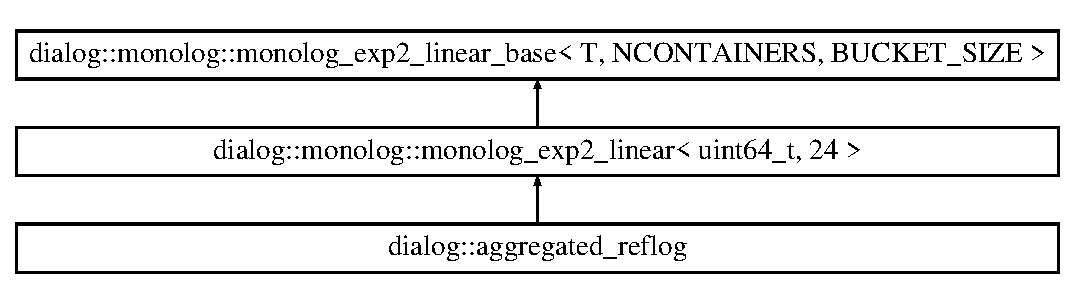
\includegraphics[height=3.000000cm]{classdialog_1_1aggregated__reflog}
\end{center}
\end{figure}
\subsection*{Public Types}
\begin{DoxyCompactItemize}
\item 
\mbox{\Hypertarget{classdialog_1_1aggregated__reflog_aae5eeea7c667555591eddee31e8c012e}\label{classdialog_1_1aggregated__reflog_aae5eeea7c667555591eddee31e8c012e}} 
typedef reflog\+::size\+\_\+type {\bfseries size\+\_\+type}
\item 
\mbox{\Hypertarget{classdialog_1_1aggregated__reflog_aa404ea1b7e6d27ecb6c323cfc7f5df61}\label{classdialog_1_1aggregated__reflog_aa404ea1b7e6d27ecb6c323cfc7f5df61}} 
typedef reflog\+::pos\+\_\+type {\bfseries pos\+\_\+type}
\item 
\mbox{\Hypertarget{classdialog_1_1aggregated__reflog_a1b4a9d5661f2939e12fc4099c72bc2a8}\label{classdialog_1_1aggregated__reflog_a1b4a9d5661f2939e12fc4099c72bc2a8}} 
typedef reflog\+::value\+\_\+type {\bfseries value\+\_\+type}
\item 
\mbox{\Hypertarget{classdialog_1_1aggregated__reflog_a1368b37e03c37fee2c151f2174a84af7}\label{classdialog_1_1aggregated__reflog_a1368b37e03c37fee2c151f2174a84af7}} 
typedef reflog\+::difference\+\_\+type {\bfseries difference\+\_\+type}
\item 
\mbox{\Hypertarget{classdialog_1_1aggregated__reflog_a8c47fc7588dfbdce11a238465495c618}\label{classdialog_1_1aggregated__reflog_a8c47fc7588dfbdce11a238465495c618}} 
typedef reflog\+::pointer {\bfseries pointer}
\item 
\mbox{\Hypertarget{classdialog_1_1aggregated__reflog_a88d53700cd6f29d91e316c5c81c1ea54}\label{classdialog_1_1aggregated__reflog_a88d53700cd6f29d91e316c5c81c1ea54}} 
typedef reflog\+::reference {\bfseries reference}
\item 
\mbox{\Hypertarget{classdialog_1_1aggregated__reflog_aab249e03c122358fd4f19fb2379371dc}\label{classdialog_1_1aggregated__reflog_aab249e03c122358fd4f19fb2379371dc}} 
typedef \hyperlink{classdialog_1_1monolog_1_1monolog__iterator}{reflog\+::iterator} {\bfseries iterator}
\item 
\mbox{\Hypertarget{classdialog_1_1aggregated__reflog_ad5ca649de43391e8fa296576edaf3a80}\label{classdialog_1_1aggregated__reflog_ad5ca649de43391e8fa296576edaf3a80}} 
typedef \hyperlink{classdialog_1_1monolog_1_1monolog__iterator}{reflog\+::const\+\_\+iterator} {\bfseries const\+\_\+iterator}
\end{DoxyCompactItemize}
\subsection*{Public Member Functions}
\begin{DoxyCompactItemize}
\item 
\mbox{\Hypertarget{classdialog_1_1aggregated__reflog_a9f147eea512b45937d1594a9e71d1ec2}\label{classdialog_1_1aggregated__reflog_a9f147eea512b45937d1594a9e71d1ec2}} 
{\bfseries aggregated\+\_\+reflog} (const \hyperlink{classdialog_1_1monolog_1_1monolog__exp2__linear}{trigger\+\_\+log} \&triggers)
\item 
\mbox{\Hypertarget{classdialog_1_1aggregated__reflog_a5a81c6f3c706939b6b01e5be033c4d30}\label{classdialog_1_1aggregated__reflog_a5a81c6f3c706939b6b01e5be033c4d30}} 
void {\bfseries update\+\_\+aggregate} (int thread\+\_\+id, size\+\_\+t trigger\+\_\+id, const \hyperlink{classdialog_1_1numeric}{numeric} \&value, uint64\+\_\+t version)
\item 
\mbox{\Hypertarget{classdialog_1_1aggregated__reflog_a66d8a6b5f325dc0310cafddc8a76b2a0}\label{classdialog_1_1aggregated__reflog_a66d8a6b5f325dc0310cafddc8a76b2a0}} 
\hyperlink{classdialog_1_1numeric}{numeric} {\bfseries get\+\_\+aggregate} (size\+\_\+t trigger\+\_\+id, uint64\+\_\+t version) const
\item 
\mbox{\Hypertarget{classdialog_1_1aggregated__reflog_adb7909e37a83c8ad9fb727c4b338392e}\label{classdialog_1_1aggregated__reflog_adb7909e37a83c8ad9fb727c4b338392e}} 
size\+\_\+t {\bfseries num\+\_\+aggregates} () const
\end{DoxyCompactItemize}
\subsection*{Additional Inherited Members}


The documentation for this class was generated from the following file\+:\begin{DoxyCompactItemize}
\item 
/\+Users/neil/\+Documents/\+Berkeley/research/dialog/libdialog/dialog/aggregated\+\_\+reflog.\+h\end{DoxyCompactItemize}

\hypertarget{structdialog_1_1aggregator}{}\section{dialog\+:\+:aggregator Struct Reference}
\label{structdialog_1_1aggregator}\index{dialog\+::aggregator@{dialog\+::aggregator}}
\subsection*{Public Attributes}
\begin{DoxyCompactItemize}
\item 
\mbox{\Hypertarget{structdialog_1_1aggregator_a5a91547695c27e0a3d0cfc9a75dbd2ca}\label{structdialog_1_1aggregator_a5a91547695c27e0a3d0cfc9a75dbd2ca}} 
aggregate\+\_\+fn {\bfseries agg}
\item 
\mbox{\Hypertarget{structdialog_1_1aggregator_a620248277a8e4654c9f66b2b5deb7cbe}\label{structdialog_1_1aggregator_a620248277a8e4654c9f66b2b5deb7cbe}} 
zero\+\_\+fn {\bfseries zero}
\end{DoxyCompactItemize}


The documentation for this struct was generated from the following file\+:\begin{DoxyCompactItemize}
\item 
/\+Users/neil/\+Documents/\+Berkeley/research/dialog/libdialog/dialog/aggregate\+\_\+ops.\+h\end{DoxyCompactItemize}

\hypertarget{structdialog_1_1monitor_1_1alert}{}\section{dialog\+:\+:monitor\+:\+:alert Struct Reference}
\label{structdialog_1_1monitor_1_1alert}\index{dialog\+::monitor\+::alert@{dialog\+::monitor\+::alert}}
\subsection*{Public Member Functions}
\begin{DoxyCompactItemize}
\item 
\mbox{\Hypertarget{structdialog_1_1monitor_1_1alert_a0ae82c582ba7befbc7574ff69815d29a}\label{structdialog_1_1monitor_1_1alert_a0ae82c582ba7befbc7574ff69815d29a}} 
{\bfseries alert} (uint64\+\_\+t \+\_\+time\+\_\+bucket, const std\+::string \&trigger\+\_\+name, const std\+::string \&trigger\+\_\+expr, const \hyperlink{classdialog_1_1numeric}{numeric} \&\+\_\+value, uint64\+\_\+t \+\_\+version)
\item 
\mbox{\Hypertarget{structdialog_1_1monitor_1_1alert_ad9e51dcb429cdebe3113b7ef8cb0abda}\label{structdialog_1_1monitor_1_1alert_ad9e51dcb429cdebe3113b7ef8cb0abda}} 
std\+::string {\bfseries to\+\_\+string} () const
\end{DoxyCompactItemize}
\subsection*{Public Attributes}
\begin{DoxyCompactItemize}
\item 
\mbox{\Hypertarget{structdialog_1_1monitor_1_1alert_a71b11ce6cd39b00c8b56dfd304580505}\label{structdialog_1_1monitor_1_1alert_a71b11ce6cd39b00c8b56dfd304580505}} 
std\+::string {\bfseries trigger\+\_\+name}
\item 
\mbox{\Hypertarget{structdialog_1_1monitor_1_1alert_a0727ced14d1356e68fa654e47357f9a4}\label{structdialog_1_1monitor_1_1alert_a0727ced14d1356e68fa654e47357f9a4}} 
std\+::string {\bfseries trigger\+\_\+expr}
\item 
\mbox{\Hypertarget{structdialog_1_1monitor_1_1alert_a5d5c60a87968a5069a164512af98ada6}\label{structdialog_1_1monitor_1_1alert_a5d5c60a87968a5069a164512af98ada6}} 
\hyperlink{classdialog_1_1numeric}{numeric} {\bfseries value}
\item 
\mbox{\Hypertarget{structdialog_1_1monitor_1_1alert_ae8595d8ba1806bf04a1dd37829fcab1e}\label{structdialog_1_1monitor_1_1alert_ae8595d8ba1806bf04a1dd37829fcab1e}} 
uint32\+\_\+t {\bfseries version}
\item 
\mbox{\Hypertarget{structdialog_1_1monitor_1_1alert_a93257bcb6d63d74fdfb9f2c04633f5fc}\label{structdialog_1_1monitor_1_1alert_a93257bcb6d63d74fdfb9f2c04633f5fc}} 
uint64\+\_\+t {\bfseries time\+\_\+bucket}
\end{DoxyCompactItemize}
\subsection*{Friends}
\begin{DoxyCompactItemize}
\item 
\mbox{\Hypertarget{structdialog_1_1monitor_1_1alert_a43a339406d77cab37f40aeef23d9d52e}\label{structdialog_1_1monitor_1_1alert_a43a339406d77cab37f40aeef23d9d52e}} 
bool {\bfseries operator$<$} (const \hyperlink{structdialog_1_1monitor_1_1alert}{alert} \&left, const \hyperlink{structdialog_1_1monitor_1_1alert}{alert} \&right)
\end{DoxyCompactItemize}


The documentation for this struct was generated from the following file\+:\begin{DoxyCompactItemize}
\item 
/\+Users/neil/\+Documents/\+Berkeley/research/dialog/libdialog/dialog/alert.\+h\end{DoxyCompactItemize}

\hypertarget{classdialog_1_1monitor_1_1alert__index}{}\section{dialog\+:\+:monitor\+:\+:alert\+\_\+index Class Reference}
\label{classdialog_1_1monitor_1_1alert__index}\index{dialog\+::monitor\+::alert\+\_\+index@{dialog\+::monitor\+::alert\+\_\+index}}
\subsection*{Public Types}
\begin{DoxyCompactItemize}
\item 
\mbox{\Hypertarget{classdialog_1_1monitor_1_1alert__index_a5bcff590f4b2b262d73459775d1191d5}\label{classdialog_1_1monitor_1_1alert__index_a5bcff590f4b2b262d73459775d1191d5}} 
typedef \hyperlink{classdialog_1_1monolog_1_1monolog__exp2__linear}{monolog\+::monolog\+\_\+exp2\+\_\+linear}$<$ \hyperlink{structdialog_1_1monitor_1_1alert}{alert} $>$ {\bfseries alert\+\_\+log}
\item 
\mbox{\Hypertarget{classdialog_1_1monitor_1_1alert__index_a53eb21bd9f555ededdd34215d335dd1b}\label{classdialog_1_1monitor_1_1alert__index_a53eb21bd9f555ededdd34215d335dd1b}} 
typedef \hyperlink{classdialog_1_1index_1_1radix__tree}{index\+::radix\+\_\+tree}$<$ \hyperlink{classdialog_1_1monolog_1_1monolog__exp2__linear}{alert\+\_\+log} $>$ {\bfseries idx\+\_\+t}
\item 
\mbox{\Hypertarget{classdialog_1_1monitor_1_1alert__index_aaa5a77021b5c3bd07f3dc71250c7a1fc}\label{classdialog_1_1monitor_1_1alert__index_aaa5a77021b5c3bd07f3dc71250c7a1fc}} 
typedef \hyperlink{classflattened__container}{idx\+\_\+t\+::rt\+\_\+result} {\bfseries alert\+\_\+list}
\end{DoxyCompactItemize}
\subsection*{Public Member Functions}
\begin{DoxyCompactItemize}
\item 
\mbox{\Hypertarget{classdialog_1_1monitor_1_1alert__index_aae17c973f4fe58b96ab27adb26b9bdc3}\label{classdialog_1_1monitor_1_1alert__index_aae17c973f4fe58b96ab27adb26b9bdc3}} 
void {\bfseries add\+\_\+alert} (uint64\+\_\+t time\+\_\+bucket, const std\+::string \&trigger\+\_\+name, const std\+::string \&trigger\+\_\+expr, const \hyperlink{classdialog_1_1numeric}{numeric} \&value, uint64\+\_\+t version)
\item 
\mbox{\Hypertarget{classdialog_1_1monitor_1_1alert__index_a07e96cf06909185b98b03e061ca91e8d}\label{classdialog_1_1monitor_1_1alert__index_a07e96cf06909185b98b03e061ca91e8d}} 
\hyperlink{classflattened__container}{alert\+\_\+list} {\bfseries get\+\_\+alerts} (uint64\+\_\+t t1, uint64\+\_\+t t2) const
\end{DoxyCompactItemize}


The documentation for this class was generated from the following file\+:\begin{DoxyCompactItemize}
\item 
/\+Users/neil/\+Documents/\+Berkeley/research/dialog/libdialog/dialog/alert\+\_\+index.\+h\end{DoxyCompactItemize}

\hypertarget{classdialog_1_1bitmap}{}\section{dialog\+:\+:bitmap Class Reference}
\label{classdialog_1_1bitmap}\index{dialog\+::bitmap@{dialog\+::bitmap}}
Inheritance diagram for dialog\+:\+:bitmap\+:\begin{figure}[H]
\begin{center}
\leavevmode
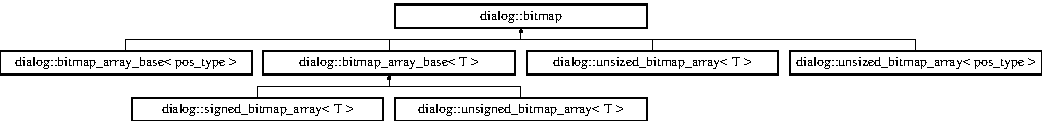
\includegraphics[height=1.621622cm]{classdialog_1_1bitmap}
\end{center}
\end{figure}
\subsection*{Public Types}
\begin{DoxyCompactItemize}
\item 
\mbox{\Hypertarget{classdialog_1_1bitmap_a9dad89abbacbfbf01882b42d105f8eab}\label{classdialog_1_1bitmap_a9dad89abbacbfbf01882b42d105f8eab}} 
typedef size\+\_\+t {\bfseries pos\+\_\+type}
\item 
\mbox{\Hypertarget{classdialog_1_1bitmap_a1f43213dbbee2916b2300f18cc0cf8e4}\label{classdialog_1_1bitmap_a1f43213dbbee2916b2300f18cc0cf8e4}} 
typedef size\+\_\+t {\bfseries size\+\_\+type}
\item 
\mbox{\Hypertarget{classdialog_1_1bitmap_a581f5b4b805e7227daff300d3e6889a1}\label{classdialog_1_1bitmap_a581f5b4b805e7227daff300d3e6889a1}} 
typedef uint64\+\_\+t {\bfseries data\+\_\+type}
\item 
\mbox{\Hypertarget{classdialog_1_1bitmap_a32a35c8848493dfd325db63fa5d9522b}\label{classdialog_1_1bitmap_a32a35c8848493dfd325db63fa5d9522b}} 
typedef uint8\+\_\+t {\bfseries width\+\_\+type}
\end{DoxyCompactItemize}
\subsection*{Public Member Functions}
\begin{DoxyCompactItemize}
\item 
\mbox{\Hypertarget{classdialog_1_1bitmap_a24d0f574de691d0a6a49042250b70402}\label{classdialog_1_1bitmap_a24d0f574de691d0a6a49042250b70402}} 
{\bfseries bitmap} (size\+\_\+type num\+\_\+bits)
\item 
\mbox{\Hypertarget{classdialog_1_1bitmap_a0b900d1a8caeda35213c8891e092c61a}\label{classdialog_1_1bitmap_a0b900d1a8caeda35213c8891e092c61a}} 
data\+\_\+type $\ast$ {\bfseries data} ()
\item 
\mbox{\Hypertarget{classdialog_1_1bitmap_a2066fd879c2e7c3d18ff590e9f1826b8}\label{classdialog_1_1bitmap_a2066fd879c2e7c3d18ff590e9f1826b8}} 
size\+\_\+type {\bfseries num\+\_\+bits} ()
\item 
\mbox{\Hypertarget{classdialog_1_1bitmap_a560fd4286efbe1d770926a4ceccc3d9a}\label{classdialog_1_1bitmap_a560fd4286efbe1d770926a4ceccc3d9a}} 
void {\bfseries clear\+\_\+all} ()
\item 
\mbox{\Hypertarget{classdialog_1_1bitmap_abeda36a2708d0b87296f7c4322357421}\label{classdialog_1_1bitmap_abeda36a2708d0b87296f7c4322357421}} 
void {\bfseries set\+\_\+bit} (pos\+\_\+type i)
\item 
\mbox{\Hypertarget{classdialog_1_1bitmap_a60bf0ac8d398e48e8f3c467999d0b1c8}\label{classdialog_1_1bitmap_a60bf0ac8d398e48e8f3c467999d0b1c8}} 
void {\bfseries unset\+\_\+bit} (pos\+\_\+type i)
\item 
\mbox{\Hypertarget{classdialog_1_1bitmap_a50fa02f2e4a94c567f67761988c78d7f}\label{classdialog_1_1bitmap_a50fa02f2e4a94c567f67761988c78d7f}} 
bool {\bfseries get\+\_\+bit} (pos\+\_\+type i) const
\item 
\mbox{\Hypertarget{classdialog_1_1bitmap_a567ec662fb5fa68399b3097cc63c44ea}\label{classdialog_1_1bitmap_a567ec662fb5fa68399b3097cc63c44ea}} 
{\footnotesize template$<$typename T $>$ }\\std\+::enable\+\_\+if$<$ std\+::is\+\_\+arithmetic$<$ T $>$\+::value $>$\+::type {\bfseries set\+\_\+val\+\_\+pos} (pos\+\_\+type pos, T val, width\+\_\+type bits)
\item 
\mbox{\Hypertarget{classdialog_1_1bitmap_aa56b2e9be38fd068ac374f2f7a33120b}\label{classdialog_1_1bitmap_aa56b2e9be38fd068ac374f2f7a33120b}} 
{\footnotesize template$<$typename T $>$ }\\std\+::enable\+\_\+if$<$ std\+::is\+\_\+arithmetic$<$ T $>$\+::value, T $>$\+::type {\bfseries get\+\_\+val\+\_\+pos} (pos\+\_\+type pos, width\+\_\+type bits) const
\item 
\mbox{\Hypertarget{classdialog_1_1bitmap_af93ff2660d3b790eee85692a41bdb823}\label{classdialog_1_1bitmap_af93ff2660d3b790eee85692a41bdb823}} 
virtual size\+\_\+type {\bfseries serialize} (std\+::ostream \&out)
\item 
\mbox{\Hypertarget{classdialog_1_1bitmap_a5c4c9a790b785bbc021d913a53cffe80}\label{classdialog_1_1bitmap_a5c4c9a790b785bbc021d913a53cffe80}} 
virtual size\+\_\+type {\bfseries deserialize} (std\+::istream \&in)
\end{DoxyCompactItemize}
\subsection*{Protected Attributes}
\begin{DoxyCompactItemize}
\item 
\mbox{\Hypertarget{classdialog_1_1bitmap_a343e756ef501f484742f1e87a4085074}\label{classdialog_1_1bitmap_a343e756ef501f484742f1e87a4085074}} 
data\+\_\+type $\ast$ {\bfseries data\+\_\+}
\item 
\mbox{\Hypertarget{classdialog_1_1bitmap_a85885c54fdd3eec34785d882bc4d3228}\label{classdialog_1_1bitmap_a85885c54fdd3eec34785d882bc4d3228}} 
size\+\_\+type {\bfseries size\+\_\+}
\end{DoxyCompactItemize}


The documentation for this class was generated from the following file\+:\begin{DoxyCompactItemize}
\item 
/\+Users/neil/\+Documents/\+Berkeley/research/dialog/libdialog/dialog/bitmap.\+h\end{DoxyCompactItemize}

\hypertarget{classdialog_1_1bitmap__array__base}{}\section{dialog\+:\+:bitmap\+\_\+array\+\_\+base$<$ T $>$ Class Template Reference}
\label{classdialog_1_1bitmap__array__base}\index{dialog\+::bitmap\+\_\+array\+\_\+base$<$ T $>$@{dialog\+::bitmap\+\_\+array\+\_\+base$<$ T $>$}}
Inheritance diagram for dialog\+:\+:bitmap\+\_\+array\+\_\+base$<$ T $>$\+:\begin{figure}[H]
\begin{center}
\leavevmode
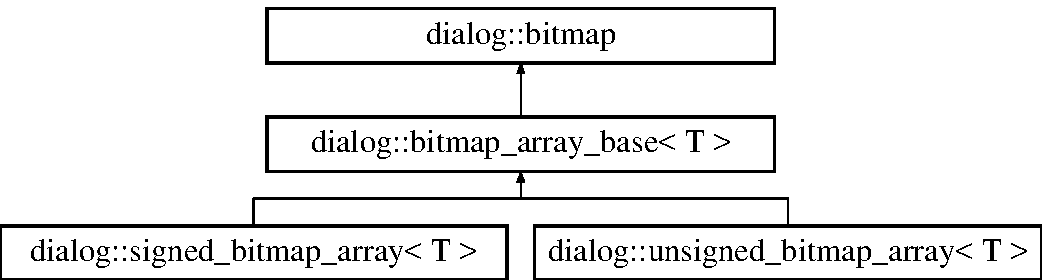
\includegraphics[height=3.000000cm]{classdialog_1_1bitmap__array__base}
\end{center}
\end{figure}
\subsection*{Public Member Functions}
\begin{DoxyCompactItemize}
\item 
\mbox{\Hypertarget{classdialog_1_1bitmap__array__base_ab6b857655a8de2706653b5a7996a625b}\label{classdialog_1_1bitmap__array__base_ab6b857655a8de2706653b5a7996a625b}} 
{\bfseries bitmap\+\_\+array\+\_\+base} (const \hyperlink{classdialog_1_1bitmap__array__base}{bitmap\+\_\+array\+\_\+base} \&array)
\item 
\mbox{\Hypertarget{classdialog_1_1bitmap__array__base_ac60cc574d5908417b53bfbd7a5809626}\label{classdialog_1_1bitmap__array__base_ac60cc574d5908417b53bfbd7a5809626}} 
{\bfseries bitmap\+\_\+array\+\_\+base} (size\+\_\+type num\+\_\+elements, width\+\_\+type bit\+\_\+width)
\item 
\mbox{\Hypertarget{classdialog_1_1bitmap__array__base_a9bbb84f69a124c0a3b654e8570833fd8}\label{classdialog_1_1bitmap__array__base_a9bbb84f69a124c0a3b654e8570833fd8}} 
size\+\_\+type {\bfseries size} () const
\item 
\mbox{\Hypertarget{classdialog_1_1bitmap__array__base_ada6add4a94341c88dc41de234b090ccb}\label{classdialog_1_1bitmap__array__base_ada6add4a94341c88dc41de234b090ccb}} 
width\+\_\+type {\bfseries bit\+\_\+width} () const
\item 
\mbox{\Hypertarget{classdialog_1_1bitmap__array__base_ab7816447c88267c25987ad45ceb65a5e}\label{classdialog_1_1bitmap__array__base_ab7816447c88267c25987ad45ceb65a5e}} 
bool {\bfseries empty} () const
\item 
virtual size\+\_\+type \hyperlink{classdialog_1_1bitmap__array__base_aa7a0aa644a5a37eaf87a902a20cee939}{serialize} (std\+::ostream \&out) override
\item 
virtual size\+\_\+type \hyperlink{classdialog_1_1bitmap__array__base_a51a91fced01d96475dc24e23da2d06e8}{deserialize} (std\+::istream \&in) override
\end{DoxyCompactItemize}
\subsection*{Protected Attributes}
\begin{DoxyCompactItemize}
\item 
\mbox{\Hypertarget{classdialog_1_1bitmap__array__base_a8c831f6a67020d74dc29401c0dd9bce4}\label{classdialog_1_1bitmap__array__base_a8c831f6a67020d74dc29401c0dd9bce4}} 
size\+\_\+type {\bfseries num\+\_\+elements\+\_\+}
\item 
\mbox{\Hypertarget{classdialog_1_1bitmap__array__base_a63b0af9fb47d61115af1e8f1038fcb02}\label{classdialog_1_1bitmap__array__base_a63b0af9fb47d61115af1e8f1038fcb02}} 
width\+\_\+type {\bfseries bit\+\_\+width\+\_\+}
\end{DoxyCompactItemize}
\subsection*{Additional Inherited Members}


\subsection{Member Function Documentation}
\mbox{\Hypertarget{classdialog_1_1bitmap__array__base_a51a91fced01d96475dc24e23da2d06e8}\label{classdialog_1_1bitmap__array__base_a51a91fced01d96475dc24e23da2d06e8}} 
\index{dialog\+::bitmap\+\_\+array\+\_\+base@{dialog\+::bitmap\+\_\+array\+\_\+base}!deserialize@{deserialize}}
\index{deserialize@{deserialize}!dialog\+::bitmap\+\_\+array\+\_\+base@{dialog\+::bitmap\+\_\+array\+\_\+base}}
\subsubsection{\texorpdfstring{deserialize()}{deserialize()}}
{\footnotesize\ttfamily template$<$typename T$>$ \\
virtual size\+\_\+type \hyperlink{classdialog_1_1bitmap__array__base}{dialog\+::bitmap\+\_\+array\+\_\+base}$<$ T $>$\+::deserialize (\begin{DoxyParamCaption}\item[{std\+::istream \&}]{in }\end{DoxyParamCaption})\hspace{0.3cm}{\ttfamily [inline]}, {\ttfamily [override]}, {\ttfamily [virtual]}}

Deserializes bitmap from an input stream 
\begin{DoxyParams}{Parameters}
{\em in} & The input stream where the bitmap is read from \\
\hline
\end{DoxyParams}
\begin{DoxyReturn}{Returns}
The size of the data from the stream 
\end{DoxyReturn}


Reimplemented from \hyperlink{classdialog_1_1bitmap_a5c4c9a790b785bbc021d913a53cffe80}{dialog\+::bitmap}.

\mbox{\Hypertarget{classdialog_1_1bitmap__array__base_aa7a0aa644a5a37eaf87a902a20cee939}\label{classdialog_1_1bitmap__array__base_aa7a0aa644a5a37eaf87a902a20cee939}} 
\index{dialog\+::bitmap\+\_\+array\+\_\+base@{dialog\+::bitmap\+\_\+array\+\_\+base}!serialize@{serialize}}
\index{serialize@{serialize}!dialog\+::bitmap\+\_\+array\+\_\+base@{dialog\+::bitmap\+\_\+array\+\_\+base}}
\subsubsection{\texorpdfstring{serialize()}{serialize()}}
{\footnotesize\ttfamily template$<$typename T$>$ \\
virtual size\+\_\+type \hyperlink{classdialog_1_1bitmap__array__base}{dialog\+::bitmap\+\_\+array\+\_\+base}$<$ T $>$\+::serialize (\begin{DoxyParamCaption}\item[{std\+::ostream \&}]{out }\end{DoxyParamCaption})\hspace{0.3cm}{\ttfamily [inline]}, {\ttfamily [override]}, {\ttfamily [virtual]}}

Serializes bitmap to an output stream 
\begin{DoxyParams}{Parameters}
{\em out} & The output stream where the bitmap is serialized \\
\hline
\end{DoxyParams}
\begin{DoxyReturn}{Returns}
The size of the data in the stream 
\end{DoxyReturn}


Reimplemented from \hyperlink{classdialog_1_1bitmap_af93ff2660d3b790eee85692a41bdb823}{dialog\+::bitmap}.



The documentation for this class was generated from the following file\+:\begin{DoxyCompactItemize}
\item 
/\+Users/neil/\+Documents/\+Berkeley/research/dialog/libdialog/dialog/bitmap\+\_\+array.\+h\end{DoxyCompactItemize}

\hypertarget{classdialog_1_1bitmap__array__iterator}{}\section{dialog\+:\+:bitmap\+\_\+array\+\_\+iterator$<$ bitmap\+\_\+array\+\_\+impl $>$ Class Template Reference}
\label{classdialog_1_1bitmap__array__iterator}\index{dialog\+::bitmap\+\_\+array\+\_\+iterator$<$ bitmap\+\_\+array\+\_\+impl $>$@{dialog\+::bitmap\+\_\+array\+\_\+iterator$<$ bitmap\+\_\+array\+\_\+impl $>$}}
\subsection*{Public Types}
\begin{DoxyCompactItemize}
\item 
\mbox{\Hypertarget{classdialog_1_1bitmap__array__iterator_a87868981d5806d6964013d5bf25852fe}\label{classdialog_1_1bitmap__array__iterator_a87868981d5806d6964013d5bf25852fe}} 
typedef bitmap\+\_\+array\+\_\+impl\+::pos\+\_\+type {\bfseries pos\+\_\+type}
\item 
\mbox{\Hypertarget{classdialog_1_1bitmap__array__iterator_a970d92e3251b4a7efb85e5c6c2517bf3}\label{classdialog_1_1bitmap__array__iterator_a970d92e3251b4a7efb85e5c6c2517bf3}} 
typedef bitmap\+\_\+array\+\_\+impl\+::difference\+\_\+type {\bfseries difference\+\_\+type}
\item 
\mbox{\Hypertarget{classdialog_1_1bitmap__array__iterator_a690a87e957228bc2fcc46ff2fce1fa74}\label{classdialog_1_1bitmap__array__iterator_a690a87e957228bc2fcc46ff2fce1fa74}} 
typedef bitmap\+\_\+array\+\_\+impl\+::value\+\_\+type {\bfseries value\+\_\+type}
\item 
\mbox{\Hypertarget{classdialog_1_1bitmap__array__iterator_a1acce57abff5d1de76b89aaeb3178582}\label{classdialog_1_1bitmap__array__iterator_a1acce57abff5d1de76b89aaeb3178582}} 
typedef bitmap\+\_\+array\+\_\+impl\+::pointer {\bfseries pointer}
\item 
\mbox{\Hypertarget{classdialog_1_1bitmap__array__iterator_a44c587eec718b7238bb440582f2e6043}\label{classdialog_1_1bitmap__array__iterator_a44c587eec718b7238bb440582f2e6043}} 
typedef bitmap\+\_\+array\+\_\+impl\+::reference {\bfseries reference}
\item 
\mbox{\Hypertarget{classdialog_1_1bitmap__array__iterator_a635aa79f15af7f05f611ff869882e464}\label{classdialog_1_1bitmap__array__iterator_a635aa79f15af7f05f611ff869882e464}} 
typedef bitmap\+\_\+array\+\_\+impl\+::iterator\+\_\+category {\bfseries iterator\+\_\+category}
\end{DoxyCompactItemize}
\subsection*{Public Member Functions}
\begin{DoxyCompactItemize}
\item 
\mbox{\Hypertarget{classdialog_1_1bitmap__array__iterator_a150d142a00b355f4215e85e4a9b59e3b}\label{classdialog_1_1bitmap__array__iterator_a150d142a00b355f4215e85e4a9b59e3b}} 
{\bfseries bitmap\+\_\+array\+\_\+iterator} (bitmap\+\_\+array\+\_\+impl $\ast$array, pos\+\_\+type pos)
\item 
\mbox{\Hypertarget{classdialog_1_1bitmap__array__iterator_ad36d311e3de7ea61e6a2ca4f95ac9b3a}\label{classdialog_1_1bitmap__array__iterator_ad36d311e3de7ea61e6a2ca4f95ac9b3a}} 
reference {\bfseries operator$\ast$} () const
\item 
\mbox{\Hypertarget{classdialog_1_1bitmap__array__iterator_aa465184769a8ddb09aa0bccff98ede64}\label{classdialog_1_1bitmap__array__iterator_aa465184769a8ddb09aa0bccff98ede64}} 
\hyperlink{classdialog_1_1bitmap__array__iterator}{bitmap\+\_\+array\+\_\+iterator} \& {\bfseries operator++} ()
\item 
\mbox{\Hypertarget{classdialog_1_1bitmap__array__iterator_ae67c4ecf86cfdc81c9708774d303c83c}\label{classdialog_1_1bitmap__array__iterator_ae67c4ecf86cfdc81c9708774d303c83c}} 
\hyperlink{classdialog_1_1bitmap__array__iterator}{bitmap\+\_\+array\+\_\+iterator} {\bfseries operator++} (int)
\item 
\mbox{\Hypertarget{classdialog_1_1bitmap__array__iterator_a47b40b609780a709403ae34cbe3c229e}\label{classdialog_1_1bitmap__array__iterator_a47b40b609780a709403ae34cbe3c229e}} 
\hyperlink{classdialog_1_1bitmap__array__iterator}{bitmap\+\_\+array\+\_\+iterator} \& {\bfseries operator-\/-\/} ()
\item 
\mbox{\Hypertarget{classdialog_1_1bitmap__array__iterator_acfe196d8edfa16f3aa8002c982c94ac3}\label{classdialog_1_1bitmap__array__iterator_acfe196d8edfa16f3aa8002c982c94ac3}} 
\hyperlink{classdialog_1_1bitmap__array__iterator}{bitmap\+\_\+array\+\_\+iterator} {\bfseries operator-\/-\/} (int)
\item 
\mbox{\Hypertarget{classdialog_1_1bitmap__array__iterator_adefd06d5b695d87812f1239b5e4c8885}\label{classdialog_1_1bitmap__array__iterator_adefd06d5b695d87812f1239b5e4c8885}} 
\hyperlink{classdialog_1_1bitmap__array__iterator}{bitmap\+\_\+array\+\_\+iterator} \& {\bfseries operator+=} (difference\+\_\+type i)
\item 
\mbox{\Hypertarget{classdialog_1_1bitmap__array__iterator_a0287d32995730611a8c994030b7659b6}\label{classdialog_1_1bitmap__array__iterator_a0287d32995730611a8c994030b7659b6}} 
\hyperlink{classdialog_1_1bitmap__array__iterator}{bitmap\+\_\+array\+\_\+iterator} \& {\bfseries operator-\/=} (difference\+\_\+type i)
\item 
\mbox{\Hypertarget{classdialog_1_1bitmap__array__iterator_a773d69ec2ad2efe856a2586cd3f967c2}\label{classdialog_1_1bitmap__array__iterator_a773d69ec2ad2efe856a2586cd3f967c2}} 
\hyperlink{classdialog_1_1bitmap__array__iterator}{bitmap\+\_\+array\+\_\+iterator} \& {\bfseries operator=} (const \hyperlink{classdialog_1_1bitmap__array__iterator}{bitmap\+\_\+array\+\_\+iterator} \&it)
\item 
\mbox{\Hypertarget{classdialog_1_1bitmap__array__iterator_a290526a5340a971d20b323400d50dad9}\label{classdialog_1_1bitmap__array__iterator_a290526a5340a971d20b323400d50dad9}} 
\hyperlink{classdialog_1_1bitmap__array__iterator}{bitmap\+\_\+array\+\_\+iterator} {\bfseries operator+} (difference\+\_\+type i) const
\item 
\mbox{\Hypertarget{classdialog_1_1bitmap__array__iterator_a9c1e39d485bf4bb8c810dbd582f7d53f}\label{classdialog_1_1bitmap__array__iterator_a9c1e39d485bf4bb8c810dbd582f7d53f}} 
\hyperlink{classdialog_1_1bitmap__array__iterator}{bitmap\+\_\+array\+\_\+iterator} {\bfseries operator-\/} (difference\+\_\+type i) const
\item 
\mbox{\Hypertarget{classdialog_1_1bitmap__array__iterator_aa581ea05efde41ac1f1d48e85e1a88c3}\label{classdialog_1_1bitmap__array__iterator_aa581ea05efde41ac1f1d48e85e1a88c3}} 
reference {\bfseries operator\mbox{[}$\,$\mbox{]}} (difference\+\_\+type i) const
\item 
\mbox{\Hypertarget{classdialog_1_1bitmap__array__iterator_a007944cb4cf09d6b2cc5a82b2f7a9a8a}\label{classdialog_1_1bitmap__array__iterator_a007944cb4cf09d6b2cc5a82b2f7a9a8a}} 
bool {\bfseries operator==} (const \hyperlink{classdialog_1_1bitmap__array__iterator}{bitmap\+\_\+array\+\_\+iterator} \&it) const
\item 
\mbox{\Hypertarget{classdialog_1_1bitmap__array__iterator_a062078ca2a2c22c259118029616e79e6}\label{classdialog_1_1bitmap__array__iterator_a062078ca2a2c22c259118029616e79e6}} 
bool {\bfseries operator!=} (const \hyperlink{classdialog_1_1bitmap__array__iterator}{bitmap\+\_\+array\+\_\+iterator} \&it) const
\item 
\mbox{\Hypertarget{classdialog_1_1bitmap__array__iterator_a0fbd8cd35b11ad065aaa7900a17ade9f}\label{classdialog_1_1bitmap__array__iterator_a0fbd8cd35b11ad065aaa7900a17ade9f}} 
bool {\bfseries operator$<$} (const \hyperlink{classdialog_1_1bitmap__array__iterator}{bitmap\+\_\+array\+\_\+iterator} \&it) const
\item 
\mbox{\Hypertarget{classdialog_1_1bitmap__array__iterator_a15d7dcead69e0224cfd9a44c8a616118}\label{classdialog_1_1bitmap__array__iterator_a15d7dcead69e0224cfd9a44c8a616118}} 
bool {\bfseries operator$>$} (const \hyperlink{classdialog_1_1bitmap__array__iterator}{bitmap\+\_\+array\+\_\+iterator} \&it) const
\item 
\mbox{\Hypertarget{classdialog_1_1bitmap__array__iterator_a7bbfdf826b8a0b6f1877f8170713b23c}\label{classdialog_1_1bitmap__array__iterator_a7bbfdf826b8a0b6f1877f8170713b23c}} 
bool {\bfseries operator$>$=} (const \hyperlink{classdialog_1_1bitmap__array__iterator}{bitmap\+\_\+array\+\_\+iterator} \&it) const
\item 
\mbox{\Hypertarget{classdialog_1_1bitmap__array__iterator_a5ca6b5fdd801f6b29398bcd6989f4d27}\label{classdialog_1_1bitmap__array__iterator_a5ca6b5fdd801f6b29398bcd6989f4d27}} 
bool {\bfseries operator$<$=} (const \hyperlink{classdialog_1_1bitmap__array__iterator}{bitmap\+\_\+array\+\_\+iterator} \&it) const
\item 
\mbox{\Hypertarget{classdialog_1_1bitmap__array__iterator_a90b4535f4d21f04d198fb7b01f7a077c}\label{classdialog_1_1bitmap__array__iterator_a90b4535f4d21f04d198fb7b01f7a077c}} 
difference\+\_\+type {\bfseries operator-\/} (const \hyperlink{classdialog_1_1bitmap__array__iterator}{bitmap\+\_\+array\+\_\+iterator} \&it)
\end{DoxyCompactItemize}


The documentation for this class was generated from the following file\+:\begin{DoxyCompactItemize}
\item 
/\+Users/neil/\+Documents/\+Berkeley/research/dialog/libdialog/dialog/bitmap\+\_\+array.\+h\end{DoxyCompactItemize}

\hypertarget{classdialog_1_1byte__string}{}\section{dialog\+:\+:byte\+\_\+string Class Reference}
\label{classdialog_1_1byte__string}\index{dialog\+::byte\+\_\+string@{dialog\+::byte\+\_\+string}}
\subsection*{Public Member Functions}
\begin{DoxyCompactItemize}
\item 
\mbox{\Hypertarget{classdialog_1_1byte__string_a0cbac8232055b2fc1808e7ee17db3fcb}\label{classdialog_1_1byte__string_a0cbac8232055b2fc1808e7ee17db3fcb}} 
{\bfseries byte\+\_\+string} (bool val)
\item 
\mbox{\Hypertarget{classdialog_1_1byte__string_adee5703c8d59e48f08dba1ca465496e5}\label{classdialog_1_1byte__string_adee5703c8d59e48f08dba1ca465496e5}} 
{\footnotesize template$<$typename T , typename std\+::enable\+\_\+if$<$ std\+::is\+\_\+integral$<$ T $>$\+::value \&\&!std\+::is\+\_\+same$<$ T, bool $>$\+::value \&\&std\+::is\+\_\+signed$<$ T $>$\+::value, T $>$\+::type $\ast$  = nullptr$>$ }\\{\bfseries byte\+\_\+string} (T val)
\item 
\mbox{\Hypertarget{classdialog_1_1byte__string_adee5703c8d59e48f08dba1ca465496e5}\label{classdialog_1_1byte__string_adee5703c8d59e48f08dba1ca465496e5}} 
{\footnotesize template$<$typename T , typename std\+::enable\+\_\+if$<$ std\+::is\+\_\+integral$<$ T $>$\+::value \&\&!std\+::is\+\_\+same$<$ T, bool $>$\+::value \&\&!std\+::is\+\_\+signed$<$ T $>$\+::value, T $>$\+::type $\ast$  = nullptr$>$ }\\{\bfseries byte\+\_\+string} (T val)
\item 
\mbox{\Hypertarget{classdialog_1_1byte__string_a4659c01ae6b127414e6a08515e1703ed}\label{classdialog_1_1byte__string_a4659c01ae6b127414e6a08515e1703ed}} 
{\bfseries byte\+\_\+string} (const std\+::string \&str)
\item 
\mbox{\Hypertarget{classdialog_1_1byte__string_abff23d7b1170ea8804c5a444a9fe3d7c}\label{classdialog_1_1byte__string_abff23d7b1170ea8804c5a444a9fe3d7c}} 
{\bfseries byte\+\_\+string} (const std\+::string \&str, size\+\_\+t length)
\item 
\mbox{\Hypertarget{classdialog_1_1byte__string_ac3676d996837aca8e6c091e6d61ee0a4}\label{classdialog_1_1byte__string_ac3676d996837aca8e6c091e6d61ee0a4}} 
{\bfseries byte\+\_\+string} (const \hyperlink{classdialog_1_1immutable__byte__string}{immutable\+\_\+byte\+\_\+string} \&other)
\item 
\mbox{\Hypertarget{classdialog_1_1byte__string_a0005d604588a58a3c1e856716e16322a}\label{classdialog_1_1byte__string_a0005d604588a58a3c1e856716e16322a}} 
{\bfseries byte\+\_\+string} (const \hyperlink{classdialog_1_1byte__string}{byte\+\_\+string} \&other)
\item 
\mbox{\Hypertarget{classdialog_1_1byte__string_a402f3675a2d9980f528f63c21220de59}\label{classdialog_1_1byte__string_a402f3675a2d9980f528f63c21220de59}} 
{\bfseries byte\+\_\+string} (\hyperlink{classdialog_1_1byte__string}{byte\+\_\+string} \&\&other)
\item 
\mbox{\Hypertarget{classdialog_1_1byte__string_a6f0c061ba48803c47a2dc9ec88115a43}\label{classdialog_1_1byte__string_a6f0c061ba48803c47a2dc9ec88115a43}} 
uint8\+\_\+t \& {\bfseries operator\mbox{[}$\,$\mbox{]}} (size\+\_\+t idx)
\item 
\mbox{\Hypertarget{classdialog_1_1byte__string_a01d303bedcd767f619787cd480661d41}\label{classdialog_1_1byte__string_a01d303bedcd767f619787cd480661d41}} 
uint8\+\_\+t {\bfseries operator\mbox{[}$\,$\mbox{]}} (size\+\_\+t idx) const
\item 
\mbox{\Hypertarget{classdialog_1_1byte__string_ae9f2384a3e7da34f066314e59decbe9c}\label{classdialog_1_1byte__string_ae9f2384a3e7da34f066314e59decbe9c}} 
bool {\bfseries operator$<$} (const \hyperlink{classdialog_1_1byte__string}{byte\+\_\+string} \&other) const
\item 
\mbox{\Hypertarget{classdialog_1_1byte__string_aa3f9b2567f12d3efa5e41416d8a3570e}\label{classdialog_1_1byte__string_aa3f9b2567f12d3efa5e41416d8a3570e}} 
bool {\bfseries operator$<$=} (const \hyperlink{classdialog_1_1byte__string}{byte\+\_\+string} \&other) const
\item 
\mbox{\Hypertarget{classdialog_1_1byte__string_a18ca77a7d9bb8ee402df3a6c80e77f07}\label{classdialog_1_1byte__string_a18ca77a7d9bb8ee402df3a6c80e77f07}} 
bool {\bfseries operator$>$} (const \hyperlink{classdialog_1_1byte__string}{byte\+\_\+string} \&other) const
\item 
\mbox{\Hypertarget{classdialog_1_1byte__string_a384bf3938e65ef6a527cf648b586f31d}\label{classdialog_1_1byte__string_a384bf3938e65ef6a527cf648b586f31d}} 
bool {\bfseries operator$>$=} (const \hyperlink{classdialog_1_1byte__string}{byte\+\_\+string} \&other) const
\item 
\mbox{\Hypertarget{classdialog_1_1byte__string_a44640b32150fe7758298cfa45047657c}\label{classdialog_1_1byte__string_a44640b32150fe7758298cfa45047657c}} 
bool {\bfseries operator==} (const \hyperlink{classdialog_1_1byte__string}{byte\+\_\+string} \&other) const
\item 
\mbox{\Hypertarget{classdialog_1_1byte__string_ae4f19c0edb37d4344314cdee9777e09a}\label{classdialog_1_1byte__string_ae4f19c0edb37d4344314cdee9777e09a}} 
bool {\bfseries operator!=} (const \hyperlink{classdialog_1_1byte__string}{byte\+\_\+string} \&other) const
\item 
\mbox{\Hypertarget{classdialog_1_1byte__string_a2e064d4077c1b37e65f45e7b0f7696d3}\label{classdialog_1_1byte__string_a2e064d4077c1b37e65f45e7b0f7696d3}} 
\hyperlink{classdialog_1_1byte__string}{byte\+\_\+string} \& {\bfseries operator++} ()
\item 
\mbox{\Hypertarget{classdialog_1_1byte__string_a08e49ec43a7c1e23dd33756e3b246c8f}\label{classdialog_1_1byte__string_a08e49ec43a7c1e23dd33756e3b246c8f}} 
\hyperlink{classdialog_1_1byte__string}{byte\+\_\+string} \& {\bfseries operator-\/-\/} ()
\item 
\mbox{\Hypertarget{classdialog_1_1byte__string_ae00f6c37b2241c9fe633032caeb426c2}\label{classdialog_1_1byte__string_ae00f6c37b2241c9fe633032caeb426c2}} 
\hyperlink{classdialog_1_1byte__string}{byte\+\_\+string} \& {\bfseries operator=} (const \hyperlink{classdialog_1_1immutable__byte__string}{immutable\+\_\+byte\+\_\+string} \&other)
\item 
\mbox{\Hypertarget{classdialog_1_1byte__string_a9bbea0c4b365a9e4526bb5330f825bb4}\label{classdialog_1_1byte__string_a9bbea0c4b365a9e4526bb5330f825bb4}} 
\hyperlink{classdialog_1_1byte__string}{byte\+\_\+string} \& {\bfseries operator=} (const \hyperlink{classdialog_1_1byte__string}{byte\+\_\+string} \&other)
\item 
\mbox{\Hypertarget{classdialog_1_1byte__string_a8a8e4175f33663cff1c80697eda7a617}\label{classdialog_1_1byte__string_a8a8e4175f33663cff1c80697eda7a617}} 
\hyperlink{classdialog_1_1byte__string}{byte\+\_\+string} \& {\bfseries operator=} (\hyperlink{classdialog_1_1byte__string}{byte\+\_\+string} \&\&other)
\item 
\mbox{\Hypertarget{classdialog_1_1byte__string_a361caf4069c967a2ebc5370dcacb6743}\label{classdialog_1_1byte__string_a361caf4069c967a2ebc5370dcacb6743}} 
\hyperlink{classdialog_1_1immutable__byte__string}{immutable\+\_\+byte\+\_\+string} {\bfseries copy} () const
\item 
\mbox{\Hypertarget{classdialog_1_1byte__string_aa538423485c8665531412f997ff821ce}\label{classdialog_1_1byte__string_aa538423485c8665531412f997ff821ce}} 
std\+::string {\bfseries to\+\_\+string} () const
\end{DoxyCompactItemize}


The documentation for this class was generated from the following file\+:\begin{DoxyCompactItemize}
\item 
/\+Users/neil/\+Documents/\+Berkeley/research/dialog/libdialog/dialog/byte\+\_\+string.\+h\end{DoxyCompactItemize}

\hypertarget{structdialog_1_1column__snapshot}{}\section{dialog\+:\+:column\+\_\+snapshot Struct Reference}
\label{structdialog_1_1column__snapshot}\index{dialog\+::column\+\_\+snapshot@{dialog\+::column\+\_\+snapshot}}
\subsection*{Public Attributes}
\begin{DoxyCompactItemize}
\item 
\mbox{\Hypertarget{structdialog_1_1column__snapshot_a7760426f26ee1000cbe045e570ce8bb6}\label{structdialog_1_1column__snapshot_a7760426f26ee1000cbe045e570ce8bb6}} 
\hyperlink{structdialog_1_1data__type}{data\+\_\+type} {\bfseries type}
\item 
\mbox{\Hypertarget{structdialog_1_1column__snapshot_af813309cb5a6364642c786183dd28667}\label{structdialog_1_1column__snapshot_af813309cb5a6364642c786183dd28667}} 
size\+\_\+t {\bfseries offset}
\item 
\mbox{\Hypertarget{structdialog_1_1column__snapshot_a8962d53455d80d2c1544406d40d74560}\label{structdialog_1_1column__snapshot_a8962d53455d80d2c1544406d40d74560}} 
bool {\bfseries indexed}
\item 
\mbox{\Hypertarget{structdialog_1_1column__snapshot_a1ae01e36e383f8ce8fb7ebfa145e2727}\label{structdialog_1_1column__snapshot_a1ae01e36e383f8ce8fb7ebfa145e2727}} 
uint32\+\_\+t {\bfseries index\+\_\+id}
\item 
\mbox{\Hypertarget{structdialog_1_1column__snapshot_aebb28f4cf6ee211f214cc5496817239c}\label{structdialog_1_1column__snapshot_aebb28f4cf6ee211f214cc5496817239c}} 
double {\bfseries index\+\_\+bucket\+\_\+size}
\end{DoxyCompactItemize}


The documentation for this struct was generated from the following file\+:\begin{DoxyCompactItemize}
\item 
/\+Users/neil/\+Documents/\+Berkeley/research/dialog/libdialog/dialog/column\+\_\+snapshot.\+h\end{DoxyCompactItemize}

\hypertarget{classdialog_1_1column__t}{}\section{dialog\+:\+:column\+\_\+t Class Reference}
\label{classdialog_1_1column__t}\index{dialog\+::column\+\_\+t@{dialog\+::column\+\_\+t}}
\subsection*{Public Member Functions}
\begin{DoxyCompactItemize}
\item 
\hyperlink{classdialog_1_1column__t_a294bc42fee87fb4e55542bda71a98843}{column\+\_\+t} ()
\item 
\hyperlink{classdialog_1_1column__t_a90d375f7d115c8241453867ebaf36b89}{column\+\_\+t} (uint16\+\_\+t \hyperlink{classdialog_1_1column__t_aca785728bbaaced685cd2e0d6a027173}{idx}, uint16\+\_\+t \hyperlink{classdialog_1_1column__t_a3889fc0e609ebba20c9b323a194cade1}{offset}, const \hyperlink{structdialog_1_1data__type}{data\+\_\+type} \&\hyperlink{classdialog_1_1column__t_a8316411224f15b6f25c59471422ca167}{type}, const std\+::string \&\hyperlink{classdialog_1_1column__t_a2a5d9e2d2673082a96218bb3c5b335b2}{name}, const \hyperlink{classdialog_1_1mutable__value}{mutable\+\_\+value} \&\hyperlink{classdialog_1_1column__t_a2c391fd127a2cdfbb5304c618f81b0b7}{min}, const \hyperlink{classdialog_1_1mutable__value}{mutable\+\_\+value} \&\hyperlink{classdialog_1_1column__t_a1588992ac054925f217f41a0de488896}{max})
\item 
std\+::string \hyperlink{classdialog_1_1column__t_a2a5d9e2d2673082a96218bb3c5b335b2}{name} () const
\item 
const \hyperlink{structdialog_1_1data__type}{data\+\_\+type} \& \hyperlink{classdialog_1_1column__t_a8316411224f15b6f25c59471422ca167}{type} () const
\item 
uint16\+\_\+t \hyperlink{classdialog_1_1column__t_a3889fc0e609ebba20c9b323a194cade1}{offset} () const
\item 
uint16\+\_\+t \hyperlink{classdialog_1_1column__t_aca785728bbaaced685cd2e0d6a027173}{idx} () const
\item 
\hyperlink{classdialog_1_1mutable__value}{mutable\+\_\+value} \hyperlink{classdialog_1_1column__t_a2c391fd127a2cdfbb5304c618f81b0b7}{min} () const
\item 
\hyperlink{classdialog_1_1mutable__value}{mutable\+\_\+value} \hyperlink{classdialog_1_1column__t_a1588992ac054925f217f41a0de488896}{max} () const
\item 
uint16\+\_\+t \hyperlink{classdialog_1_1column__t_ac82b68223d597e807ac5bd4f5056b0c8}{index\+\_\+id} () const
\item 
double \hyperlink{classdialog_1_1column__t_aa43ce56355c469f098ebb2c5ee7d6ab9}{index\+\_\+bucket\+\_\+size} () const
\item 
bool \hyperlink{classdialog_1_1column__t_a61f7a157a27f4fa3d4a801db035e2166}{is\+\_\+indexed} () const
\item 
bool \hyperlink{classdialog_1_1column__t_ab9651b430ffa98ff36af3c643c591576}{set\+\_\+indexing} ()
\item 
void \hyperlink{classdialog_1_1column__t_a18cbf15074f6255b63438bf64d6622bf}{set\+\_\+indexed} (uint16\+\_\+t \hyperlink{classdialog_1_1column__t_ac82b68223d597e807ac5bd4f5056b0c8}{index\+\_\+id}, double bucket\+\_\+size)
\item 
void \hyperlink{classdialog_1_1column__t_abd10df62173d46d9189306cca8569494}{set\+\_\+unindexed} ()
\item 
bool \hyperlink{classdialog_1_1column__t_ad9c14144d0ca7ae53f84f9c7fe222db9}{disable\+\_\+indexing} ()
\item 
\hyperlink{structdialog_1_1field__t}{field\+\_\+t} \hyperlink{classdialog_1_1column__t_a73c2aee9091311707673a244d05cc99e}{apply} (void $\ast$\hyperlink{structdialog_1_1data}{data}) const
\item 
\mbox{\Hypertarget{classdialog_1_1column__t_a74f17c57b3b6d9947d38a84c39590369}\label{classdialog_1_1column__t_a74f17c57b3b6d9947d38a84c39590369}} 
\hyperlink{structdialog_1_1column__snapshot}{column\+\_\+snapshot} {\bfseries snapshot} () const
\end{DoxyCompactItemize}


\subsection{Constructor \& Destructor Documentation}
\mbox{\Hypertarget{classdialog_1_1column__t_a294bc42fee87fb4e55542bda71a98843}\label{classdialog_1_1column__t_a294bc42fee87fb4e55542bda71a98843}} 
\index{dialog\+::column\+\_\+t@{dialog\+::column\+\_\+t}!column\+\_\+t@{column\+\_\+t}}
\index{column\+\_\+t@{column\+\_\+t}!dialog\+::column\+\_\+t@{dialog\+::column\+\_\+t}}
\subsubsection{\texorpdfstring{column\+\_\+t()}{column\_t()}\hspace{0.1cm}{\footnotesize\ttfamily [1/2]}}
{\footnotesize\ttfamily dialog\+::column\+\_\+t\+::column\+\_\+t (\begin{DoxyParamCaption}{ }\end{DoxyParamCaption})\hspace{0.3cm}{\ttfamily [inline]}}

Default constructor for \hyperlink{classdialog_1_1column__t}{column\+\_\+t} \mbox{\Hypertarget{classdialog_1_1column__t_a90d375f7d115c8241453867ebaf36b89}\label{classdialog_1_1column__t_a90d375f7d115c8241453867ebaf36b89}} 
\index{dialog\+::column\+\_\+t@{dialog\+::column\+\_\+t}!column\+\_\+t@{column\+\_\+t}}
\index{column\+\_\+t@{column\+\_\+t}!dialog\+::column\+\_\+t@{dialog\+::column\+\_\+t}}
\subsubsection{\texorpdfstring{column\+\_\+t()}{column\_t()}\hspace{0.1cm}{\footnotesize\ttfamily [2/2]}}
{\footnotesize\ttfamily dialog\+::column\+\_\+t\+::column\+\_\+t (\begin{DoxyParamCaption}\item[{uint16\+\_\+t}]{idx,  }\item[{uint16\+\_\+t}]{offset,  }\item[{const \hyperlink{structdialog_1_1data__type}{data\+\_\+type} \&}]{type,  }\item[{const std\+::string \&}]{name,  }\item[{const \hyperlink{classdialog_1_1mutable__value}{mutable\+\_\+value} \&}]{min,  }\item[{const \hyperlink{classdialog_1_1mutable__value}{mutable\+\_\+value} \&}]{max }\end{DoxyParamCaption})\hspace{0.3cm}{\ttfamily [inline]}}

Constructor that initializes the fields of the column 
\begin{DoxyParams}{Parameters}
{\em idx} & The index of the column \\
\hline
{\em offset} & The offset for the column \\
\hline
{\em type} & The type of data the column has \\
\hline
{\em name} & The name of the column \\
\hline
{\em min} & The min value of the column \\
\hline
{\em max} & The max value of the column \\
\hline
\end{DoxyParams}


\subsection{Member Function Documentation}
\mbox{\Hypertarget{classdialog_1_1column__t_a73c2aee9091311707673a244d05cc99e}\label{classdialog_1_1column__t_a73c2aee9091311707673a244d05cc99e}} 
\index{dialog\+::column\+\_\+t@{dialog\+::column\+\_\+t}!apply@{apply}}
\index{apply@{apply}!dialog\+::column\+\_\+t@{dialog\+::column\+\_\+t}}
\subsubsection{\texorpdfstring{apply()}{apply()}}
{\footnotesize\ttfamily \hyperlink{structdialog_1_1field__t}{field\+\_\+t} dialog\+::column\+\_\+t\+::apply (\begin{DoxyParamCaption}\item[{void $\ast$}]{data }\end{DoxyParamCaption}) const\hspace{0.3cm}{\ttfamily [inline]}}

Creates column from data 
\begin{DoxyParams}{Parameters}
{\em data} & The data that the column stores \\
\hline
\end{DoxyParams}
\begin{DoxyReturn}{Returns}
The new column 
\end{DoxyReturn}
\mbox{\Hypertarget{classdialog_1_1column__t_ad9c14144d0ca7ae53f84f9c7fe222db9}\label{classdialog_1_1column__t_ad9c14144d0ca7ae53f84f9c7fe222db9}} 
\index{dialog\+::column\+\_\+t@{dialog\+::column\+\_\+t}!disable\+\_\+indexing@{disable\+\_\+indexing}}
\index{disable\+\_\+indexing@{disable\+\_\+indexing}!dialog\+::column\+\_\+t@{dialog\+::column\+\_\+t}}
\subsubsection{\texorpdfstring{disable\+\_\+indexing()}{disable\_indexing()}}
{\footnotesize\ttfamily bool dialog\+::column\+\_\+t\+::disable\+\_\+indexing (\begin{DoxyParamCaption}{ }\end{DoxyParamCaption})\hspace{0.3cm}{\ttfamily [inline]}}

Disables indexing for the column \begin{DoxyReturn}{Returns}
True if disabled false otherwise 
\end{DoxyReturn}
\mbox{\Hypertarget{classdialog_1_1column__t_aca785728bbaaced685cd2e0d6a027173}\label{classdialog_1_1column__t_aca785728bbaaced685cd2e0d6a027173}} 
\index{dialog\+::column\+\_\+t@{dialog\+::column\+\_\+t}!idx@{idx}}
\index{idx@{idx}!dialog\+::column\+\_\+t@{dialog\+::column\+\_\+t}}
\subsubsection{\texorpdfstring{idx()}{idx()}}
{\footnotesize\ttfamily uint16\+\_\+t dialog\+::column\+\_\+t\+::idx (\begin{DoxyParamCaption}{ }\end{DoxyParamCaption}) const\hspace{0.3cm}{\ttfamily [inline]}}

Gets the index \begin{DoxyReturn}{Returns}
The index of the column 
\end{DoxyReturn}
\mbox{\Hypertarget{classdialog_1_1column__t_aa43ce56355c469f098ebb2c5ee7d6ab9}\label{classdialog_1_1column__t_aa43ce56355c469f098ebb2c5ee7d6ab9}} 
\index{dialog\+::column\+\_\+t@{dialog\+::column\+\_\+t}!index\+\_\+bucket\+\_\+size@{index\+\_\+bucket\+\_\+size}}
\index{index\+\_\+bucket\+\_\+size@{index\+\_\+bucket\+\_\+size}!dialog\+::column\+\_\+t@{dialog\+::column\+\_\+t}}
\subsubsection{\texorpdfstring{index\+\_\+bucket\+\_\+size()}{index\_bucket\_size()}}
{\footnotesize\ttfamily double dialog\+::column\+\_\+t\+::index\+\_\+bucket\+\_\+size (\begin{DoxyParamCaption}{ }\end{DoxyParamCaption}) const\hspace{0.3cm}{\ttfamily [inline]}}

Gets the size of the bucket at the index \begin{DoxyReturn}{Returns}
The bucket size 
\end{DoxyReturn}
\mbox{\Hypertarget{classdialog_1_1column__t_ac82b68223d597e807ac5bd4f5056b0c8}\label{classdialog_1_1column__t_ac82b68223d597e807ac5bd4f5056b0c8}} 
\index{dialog\+::column\+\_\+t@{dialog\+::column\+\_\+t}!index\+\_\+id@{index\+\_\+id}}
\index{index\+\_\+id@{index\+\_\+id}!dialog\+::column\+\_\+t@{dialog\+::column\+\_\+t}}
\subsubsection{\texorpdfstring{index\+\_\+id()}{index\_id()}}
{\footnotesize\ttfamily uint16\+\_\+t dialog\+::column\+\_\+t\+::index\+\_\+id (\begin{DoxyParamCaption}{ }\end{DoxyParamCaption}) const\hspace{0.3cm}{\ttfamily [inline]}}

Gets the id of the column index \begin{DoxyReturn}{Returns}
The index id 
\end{DoxyReturn}
\mbox{\Hypertarget{classdialog_1_1column__t_a61f7a157a27f4fa3d4a801db035e2166}\label{classdialog_1_1column__t_a61f7a157a27f4fa3d4a801db035e2166}} 
\index{dialog\+::column\+\_\+t@{dialog\+::column\+\_\+t}!is\+\_\+indexed@{is\+\_\+indexed}}
\index{is\+\_\+indexed@{is\+\_\+indexed}!dialog\+::column\+\_\+t@{dialog\+::column\+\_\+t}}
\subsubsection{\texorpdfstring{is\+\_\+indexed()}{is\_indexed()}}
{\footnotesize\ttfamily bool dialog\+::column\+\_\+t\+::is\+\_\+indexed (\begin{DoxyParamCaption}{ }\end{DoxyParamCaption}) const\hspace{0.3cm}{\ttfamily [inline]}}

Whether the column is indexed \begin{DoxyReturn}{Returns}
True if the column is indexed, false otherwise 
\end{DoxyReturn}
\mbox{\Hypertarget{classdialog_1_1column__t_a1588992ac054925f217f41a0de488896}\label{classdialog_1_1column__t_a1588992ac054925f217f41a0de488896}} 
\index{dialog\+::column\+\_\+t@{dialog\+::column\+\_\+t}!max@{max}}
\index{max@{max}!dialog\+::column\+\_\+t@{dialog\+::column\+\_\+t}}
\subsubsection{\texorpdfstring{max()}{max()}}
{\footnotesize\ttfamily \hyperlink{classdialog_1_1mutable__value}{mutable\+\_\+value} dialog\+::column\+\_\+t\+::max (\begin{DoxyParamCaption}{ }\end{DoxyParamCaption}) const\hspace{0.3cm}{\ttfamily [inline]}}

Gets the maximum value \begin{DoxyReturn}{Returns}
The maximum value the column can hold 
\end{DoxyReturn}
\mbox{\Hypertarget{classdialog_1_1column__t_a2c391fd127a2cdfbb5304c618f81b0b7}\label{classdialog_1_1column__t_a2c391fd127a2cdfbb5304c618f81b0b7}} 
\index{dialog\+::column\+\_\+t@{dialog\+::column\+\_\+t}!min@{min}}
\index{min@{min}!dialog\+::column\+\_\+t@{dialog\+::column\+\_\+t}}
\subsubsection{\texorpdfstring{min()}{min()}}
{\footnotesize\ttfamily \hyperlink{classdialog_1_1mutable__value}{mutable\+\_\+value} dialog\+::column\+\_\+t\+::min (\begin{DoxyParamCaption}{ }\end{DoxyParamCaption}) const\hspace{0.3cm}{\ttfamily [inline]}}

Gets the min value \begin{DoxyReturn}{Returns}
The minimum value the column can hold 
\end{DoxyReturn}
\mbox{\Hypertarget{classdialog_1_1column__t_a2a5d9e2d2673082a96218bb3c5b335b2}\label{classdialog_1_1column__t_a2a5d9e2d2673082a96218bb3c5b335b2}} 
\index{dialog\+::column\+\_\+t@{dialog\+::column\+\_\+t}!name@{name}}
\index{name@{name}!dialog\+::column\+\_\+t@{dialog\+::column\+\_\+t}}
\subsubsection{\texorpdfstring{name()}{name()}}
{\footnotesize\ttfamily std\+::string dialog\+::column\+\_\+t\+::name (\begin{DoxyParamCaption}{ }\end{DoxyParamCaption}) const\hspace{0.3cm}{\ttfamily [inline]}}

Gets name \begin{DoxyReturn}{Returns}
The name of the column 
\end{DoxyReturn}
\mbox{\Hypertarget{classdialog_1_1column__t_a3889fc0e609ebba20c9b323a194cade1}\label{classdialog_1_1column__t_a3889fc0e609ebba20c9b323a194cade1}} 
\index{dialog\+::column\+\_\+t@{dialog\+::column\+\_\+t}!offset@{offset}}
\index{offset@{offset}!dialog\+::column\+\_\+t@{dialog\+::column\+\_\+t}}
\subsubsection{\texorpdfstring{offset()}{offset()}}
{\footnotesize\ttfamily uint16\+\_\+t dialog\+::column\+\_\+t\+::offset (\begin{DoxyParamCaption}{ }\end{DoxyParamCaption}) const\hspace{0.3cm}{\ttfamily [inline]}}

Gets offset \begin{DoxyReturn}{Returns}
The offset of the column data 
\end{DoxyReturn}
\mbox{\Hypertarget{classdialog_1_1column__t_a18cbf15074f6255b63438bf64d6622bf}\label{classdialog_1_1column__t_a18cbf15074f6255b63438bf64d6622bf}} 
\index{dialog\+::column\+\_\+t@{dialog\+::column\+\_\+t}!set\+\_\+indexed@{set\+\_\+indexed}}
\index{set\+\_\+indexed@{set\+\_\+indexed}!dialog\+::column\+\_\+t@{dialog\+::column\+\_\+t}}
\subsubsection{\texorpdfstring{set\+\_\+indexed()}{set\_indexed()}}
{\footnotesize\ttfamily void dialog\+::column\+\_\+t\+::set\+\_\+indexed (\begin{DoxyParamCaption}\item[{uint16\+\_\+t}]{index\+\_\+id,  }\item[{double}]{bucket\+\_\+size }\end{DoxyParamCaption})\hspace{0.3cm}{\ttfamily [inline]}}

Sets index 
\begin{DoxyParams}{Parameters}
{\em index\+\_\+id} & The id of the index \\
\hline
{\em bucket\+\_\+size} & The size of the bucket \\
\hline
\end{DoxyParams}
\mbox{\Hypertarget{classdialog_1_1column__t_ab9651b430ffa98ff36af3c643c591576}\label{classdialog_1_1column__t_ab9651b430ffa98ff36af3c643c591576}} 
\index{dialog\+::column\+\_\+t@{dialog\+::column\+\_\+t}!set\+\_\+indexing@{set\+\_\+indexing}}
\index{set\+\_\+indexing@{set\+\_\+indexing}!dialog\+::column\+\_\+t@{dialog\+::column\+\_\+t}}
\subsubsection{\texorpdfstring{set\+\_\+indexing()}{set\_indexing()}}
{\footnotesize\ttfamily bool dialog\+::column\+\_\+t\+::set\+\_\+indexing (\begin{DoxyParamCaption}{ }\end{DoxyParamCaption})\hspace{0.3cm}{\ttfamily [inline]}}

Index the column \begin{DoxyReturn}{Returns}
True if the column was successfully indexed, false otherwise 
\end{DoxyReturn}
\mbox{\Hypertarget{classdialog_1_1column__t_abd10df62173d46d9189306cca8569494}\label{classdialog_1_1column__t_abd10df62173d46d9189306cca8569494}} 
\index{dialog\+::column\+\_\+t@{dialog\+::column\+\_\+t}!set\+\_\+unindexed@{set\+\_\+unindexed}}
\index{set\+\_\+unindexed@{set\+\_\+unindexed}!dialog\+::column\+\_\+t@{dialog\+::column\+\_\+t}}
\subsubsection{\texorpdfstring{set\+\_\+unindexed()}{set\_unindexed()}}
{\footnotesize\ttfamily void dialog\+::column\+\_\+t\+::set\+\_\+unindexed (\begin{DoxyParamCaption}{ }\end{DoxyParamCaption})\hspace{0.3cm}{\ttfamily [inline]}}

Unindexes the column \mbox{\Hypertarget{classdialog_1_1column__t_a8316411224f15b6f25c59471422ca167}\label{classdialog_1_1column__t_a8316411224f15b6f25c59471422ca167}} 
\index{dialog\+::column\+\_\+t@{dialog\+::column\+\_\+t}!type@{type}}
\index{type@{type}!dialog\+::column\+\_\+t@{dialog\+::column\+\_\+t}}
\subsubsection{\texorpdfstring{type()}{type()}}
{\footnotesize\ttfamily const \hyperlink{structdialog_1_1data__type}{data\+\_\+type}\& dialog\+::column\+\_\+t\+::type (\begin{DoxyParamCaption}{ }\end{DoxyParamCaption}) const\hspace{0.3cm}{\ttfamily [inline]}}

Gets type \begin{DoxyReturn}{Returns}
The type of the data the column has 
\end{DoxyReturn}


The documentation for this class was generated from the following file\+:\begin{DoxyCompactItemize}
\item 
/\+Users/neil/\+Documents/\+Berkeley/research/dialog/libdialog/dialog/column.\+h\end{DoxyCompactItemize}

\hypertarget{structdialog_1_1compiled__expression}{}\section{dialog\+:\+:compiled\+\_\+expression Struct Reference}
\label{structdialog_1_1compiled__expression}\index{dialog\+::compiled\+\_\+expression@{dialog\+::compiled\+\_\+expression}}
Inheritance diagram for dialog\+:\+:compiled\+\_\+expression\+:\begin{figure}[H]
\begin{center}
\leavevmode
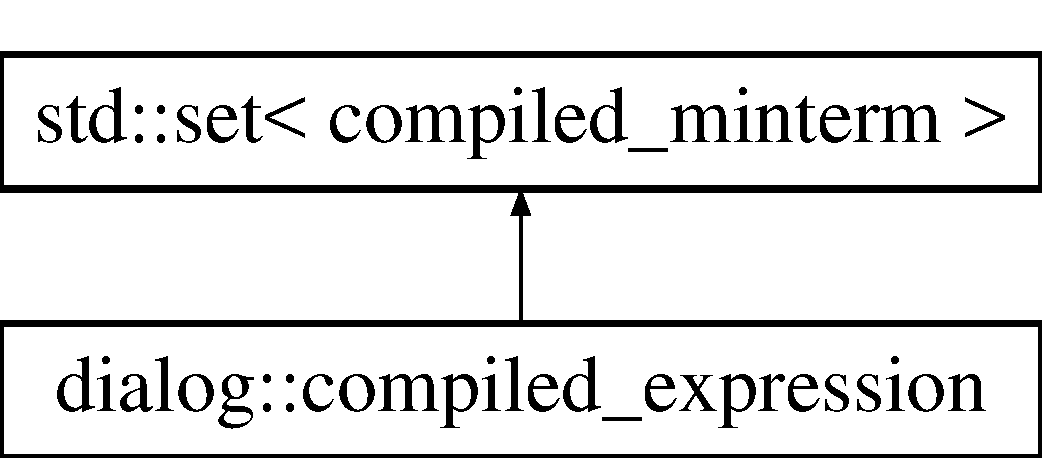
\includegraphics[height=2.000000cm]{structdialog_1_1compiled__expression}
\end{center}
\end{figure}
\subsection*{Public Member Functions}
\begin{DoxyCompactItemize}
\item 
\mbox{\Hypertarget{structdialog_1_1compiled__expression_a1fd26bfda42b0d13436f1eb9312b9db2}\label{structdialog_1_1compiled__expression_a1fd26bfda42b0d13436f1eb9312b9db2}} 
bool {\bfseries test} (const \hyperlink{structdialog_1_1record__t}{record\+\_\+t} \&r) const
\item 
\mbox{\Hypertarget{structdialog_1_1compiled__expression_a45a50c874a5c3b439d03b1f1addf9829}\label{structdialog_1_1compiled__expression_a45a50c874a5c3b439d03b1f1addf9829}} 
bool {\bfseries test} (const \hyperlink{classdialog_1_1schema__snapshot}{schema\+\_\+snapshot} \&snap, void $\ast$\hyperlink{structdialog_1_1data}{data}) const
\item 
\mbox{\Hypertarget{structdialog_1_1compiled__expression_ae4160ae052c56fcf76ad65ad5a4135ee}\label{structdialog_1_1compiled__expression_ae4160ae052c56fcf76ad65ad5a4135ee}} 
std\+::string {\bfseries to\+\_\+string} () const
\end{DoxyCompactItemize}


The documentation for this struct was generated from the following file\+:\begin{DoxyCompactItemize}
\item 
/\+Users/neil/\+Documents/\+Berkeley/research/dialog/libdialog/dialog/compiled\+\_\+expression.\+h\end{DoxyCompactItemize}

\hypertarget{structdialog_1_1compiled__minterm}{}\section{dialog\+:\+:compiled\+\_\+minterm Struct Reference}
\label{structdialog_1_1compiled__minterm}\index{dialog\+::compiled\+\_\+minterm@{dialog\+::compiled\+\_\+minterm}}
\subsection*{Public Types}
\begin{DoxyCompactItemize}
\item 
\mbox{\Hypertarget{structdialog_1_1compiled__minterm_ac790c95326bfbde518899202a42db0d5}\label{structdialog_1_1compiled__minterm_ac790c95326bfbde518899202a42db0d5}} 
typedef std\+::set$<$ \hyperlink{structdialog_1_1compiled__predicate}{compiled\+\_\+predicate} $>$\+::iterator {\bfseries iterator}
\item 
\mbox{\Hypertarget{structdialog_1_1compiled__minterm_a37352ef984da3a751ab3b9bc2642b983}\label{structdialog_1_1compiled__minterm_a37352ef984da3a751ab3b9bc2642b983}} 
typedef std\+::set$<$ \hyperlink{structdialog_1_1compiled__predicate}{compiled\+\_\+predicate} $>$\+::const\+\_\+iterator {\bfseries const\+\_\+iterator}
\end{DoxyCompactItemize}
\subsection*{Public Member Functions}
\begin{DoxyCompactItemize}
\item 
\mbox{\Hypertarget{structdialog_1_1compiled__minterm_afdd934342e641b4071097f0029f24dda}\label{structdialog_1_1compiled__minterm_afdd934342e641b4071097f0029f24dda}} 
{\bfseries compiled\+\_\+minterm} (const \hyperlink{structdialog_1_1compiled__minterm}{compiled\+\_\+minterm} \&other)
\item 
\mbox{\Hypertarget{structdialog_1_1compiled__minterm_a99bbaa3ee102bac991c7f5b9462ea6db}\label{structdialog_1_1compiled__minterm_a99bbaa3ee102bac991c7f5b9462ea6db}} 
void {\bfseries add} (const \hyperlink{structdialog_1_1compiled__predicate}{compiled\+\_\+predicate} \&p)
\item 
\mbox{\Hypertarget{structdialog_1_1compiled__minterm_ad585db052a283a82ac0427bdfb08d84a}\label{structdialog_1_1compiled__minterm_ad585db052a283a82ac0427bdfb08d84a}} 
bool {\bfseries test} (const \hyperlink{structdialog_1_1record__t}{record\+\_\+t} \&r) const
\item 
\mbox{\Hypertarget{structdialog_1_1compiled__minterm_ad5ef016f44dd9ae9b07c0c024d88b7bc}\label{structdialog_1_1compiled__minterm_ad5ef016f44dd9ae9b07c0c024d88b7bc}} 
bool {\bfseries test} (const \hyperlink{classdialog_1_1schema__snapshot}{schema\+\_\+snapshot} \&snap, void $\ast$\hyperlink{structdialog_1_1data}{data}) const
\item 
\mbox{\Hypertarget{structdialog_1_1compiled__minterm_a6bed1df725695a4e1d65939d26d6a08f}\label{structdialog_1_1compiled__minterm_a6bed1df725695a4e1d65939d26d6a08f}} 
std\+::string {\bfseries to\+\_\+string} () const
\item 
\mbox{\Hypertarget{structdialog_1_1compiled__minterm_a618e489971929f887b6645e47fc6a659}\label{structdialog_1_1compiled__minterm_a618e489971929f887b6645e47fc6a659}} 
iterator {\bfseries begin} ()
\item 
\mbox{\Hypertarget{structdialog_1_1compiled__minterm_a327e06d044a3ba799ee1a7793e6c28a7}\label{structdialog_1_1compiled__minterm_a327e06d044a3ba799ee1a7793e6c28a7}} 
iterator {\bfseries end} ()
\item 
\mbox{\Hypertarget{structdialog_1_1compiled__minterm_a5cf5c964cbaca5379729aa6adcc4cc7d}\label{structdialog_1_1compiled__minterm_a5cf5c964cbaca5379729aa6adcc4cc7d}} 
const\+\_\+iterator {\bfseries begin} () const
\item 
\mbox{\Hypertarget{structdialog_1_1compiled__minterm_a87ceaaaa066ba37c9011ce8c2528df05}\label{structdialog_1_1compiled__minterm_a87ceaaaa066ba37c9011ce8c2528df05}} 
const\+\_\+iterator {\bfseries end} () const
\item 
\mbox{\Hypertarget{structdialog_1_1compiled__minterm_a3372a6038c5355f380777819a7c20ac7}\label{structdialog_1_1compiled__minterm_a3372a6038c5355f380777819a7c20ac7}} 
bool {\bfseries operator$<$} (const \hyperlink{structdialog_1_1compiled__minterm}{compiled\+\_\+minterm} \&other) const
\item 
\mbox{\Hypertarget{structdialog_1_1compiled__minterm_abd22f6677acd5ec7918653ba8bbd2692}\label{structdialog_1_1compiled__minterm_abd22f6677acd5ec7918653ba8bbd2692}} 
size\+\_\+t {\bfseries size} () const
\end{DoxyCompactItemize}


The documentation for this struct was generated from the following file\+:\begin{DoxyCompactItemize}
\item 
/\+Users/neil/\+Documents/\+Berkeley/research/dialog/libdialog/dialog/compiled\+\_\+minterm.\+h\end{DoxyCompactItemize}

\hypertarget{structdialog_1_1compiled__predicate}{}\section{dialog\+:\+:compiled\+\_\+predicate Struct Reference}
\label{structdialog_1_1compiled__predicate}\index{dialog\+::compiled\+\_\+predicate@{dialog\+::compiled\+\_\+predicate}}
\subsection*{Public Member Functions}
\begin{DoxyCompactItemize}
\item 
\mbox{\Hypertarget{structdialog_1_1compiled__predicate_a44485c03ea9069ef8d3c7a4950d56ab3}\label{structdialog_1_1compiled__predicate_a44485c03ea9069ef8d3c7a4950d56ab3}} 
{\bfseries compiled\+\_\+predicate} (const \hyperlink{structdialog_1_1predicate__t}{predicate\+\_\+t} \&p, const \hyperlink{classdialog_1_1schema__t}{schema\+\_\+t} \&s)
\item 
\mbox{\Hypertarget{structdialog_1_1compiled__predicate_ab73cd9324b4e327ab240b8c18e2e3610}\label{structdialog_1_1compiled__predicate_ab73cd9324b4e327ab240b8c18e2e3610}} 
\hyperlink{structdialog_1_1data__type}{data\+\_\+type} {\bfseries field\+\_\+type} () const
\item 
\mbox{\Hypertarget{structdialog_1_1compiled__predicate_a31867e1b851961ed8ae901896ab3b1ef}\label{structdialog_1_1compiled__predicate_a31867e1b851961ed8ae901896ab3b1ef}} 
std\+::string {\bfseries field\+\_\+name} () const
\item 
\mbox{\Hypertarget{structdialog_1_1compiled__predicate_a98b98e5a033986b1505d822c80abbb3c}\label{structdialog_1_1compiled__predicate_a98b98e5a033986b1505d822c80abbb3c}} 
uint32\+\_\+t {\bfseries field\+\_\+idx} () const
\item 
\mbox{\Hypertarget{structdialog_1_1compiled__predicate_a32d6d0fa858a95d31364b0423c80a92f}\label{structdialog_1_1compiled__predicate_a32d6d0fa858a95d31364b0423c80a92f}} 
relop\+\_\+id {\bfseries op} () const
\item 
\mbox{\Hypertarget{structdialog_1_1compiled__predicate_af5168fc9bb40ec7ddf7f1ab4e5127269}\label{structdialog_1_1compiled__predicate_af5168fc9bb40ec7ddf7f1ab4e5127269}} 
\hyperlink{classdialog_1_1immutable__value}{immutable\+\_\+value} {\bfseries value} () const
\item 
\mbox{\Hypertarget{structdialog_1_1compiled__predicate_a8fe898956dcfdc8a1160958bbe1a7a37}\label{structdialog_1_1compiled__predicate_a8fe898956dcfdc8a1160958bbe1a7a37}} 
bool {\bfseries is\+\_\+indexed} () const
\item 
\mbox{\Hypertarget{structdialog_1_1compiled__predicate_a9cae9afd849af64a32f426c0666e546c}\label{structdialog_1_1compiled__predicate_a9cae9afd849af64a32f426c0666e546c}} 
std\+::vector$<$ \hyperlink{classdialog_1_1index__filter}{index\+\_\+filter} $>$ {\bfseries idx\+\_\+filters} () const
\item 
\mbox{\Hypertarget{structdialog_1_1compiled__predicate_a39bd0649c3a0f106a23f4ffed196df61}\label{structdialog_1_1compiled__predicate_a39bd0649c3a0f106a23f4ffed196df61}} 
bool {\bfseries test} (const \hyperlink{structdialog_1_1record__t}{record\+\_\+t} \&r) const
\item 
\mbox{\Hypertarget{structdialog_1_1compiled__predicate_ab31a2a631a339b9577d1d857d3e2efd4}\label{structdialog_1_1compiled__predicate_ab31a2a631a339b9577d1d857d3e2efd4}} 
bool {\bfseries test} (const \hyperlink{classdialog_1_1schema__snapshot}{schema\+\_\+snapshot} \&snap, void $\ast$\hyperlink{structdialog_1_1data}{data}) const
\item 
\mbox{\Hypertarget{structdialog_1_1compiled__predicate_aa5604b12d413a960d291b7366dcf8657}\label{structdialog_1_1compiled__predicate_aa5604b12d413a960d291b7366dcf8657}} 
std\+::string {\bfseries to\+\_\+string} () const
\item 
\mbox{\Hypertarget{structdialog_1_1compiled__predicate_a3098d821886e26e2bb95082b544cfede}\label{structdialog_1_1compiled__predicate_a3098d821886e26e2bb95082b544cfede}} 
bool {\bfseries operator$<$} (const \hyperlink{structdialog_1_1compiled__predicate}{compiled\+\_\+predicate} \&other) const
\end{DoxyCompactItemize}


The documentation for this struct was generated from the following file\+:\begin{DoxyCompactItemize}
\item 
/\+Users/neil/\+Documents/\+Berkeley/research/dialog/libdialog/dialog/compiled\+\_\+predicate.\+h\end{DoxyCompactItemize}

\hypertarget{classdialog_1_1configuration__params}{}\section{dialog\+:\+:configuration\+\_\+params Class Reference}
\label{classdialog_1_1configuration__params}\index{dialog\+::configuration\+\_\+params@{dialog\+::configuration\+\_\+params}}
\subsection*{Static Public Attributes}
\begin{DoxyCompactItemize}
\item 
static int {\bfseries M\+A\+X\+\_\+\+C\+O\+N\+C\+U\+R\+R\+E\+N\+CY}
\item 
static double {\bfseries I\+N\+D\+E\+X\+\_\+\+B\+U\+C\+K\+E\+T\+\_\+\+S\+I\+ZE}
\item 
static uint64\+\_\+t {\bfseries T\+I\+M\+E\+\_\+\+R\+E\+S\+O\+L\+U\+T\+I\+O\+N\+\_\+\+NS}
\item 
static uint64\+\_\+t {\bfseries M\+O\+N\+I\+T\+O\+R\+\_\+\+W\+I\+N\+D\+O\+W\+\_\+\+MS}
\item 
static uint64\+\_\+t {\bfseries M\+O\+N\+I\+T\+O\+R\+\_\+\+P\+E\+R\+I\+O\+D\+I\+C\+I\+T\+Y\+\_\+\+MS}
\end{DoxyCompactItemize}


\subsection{Member Data Documentation}
\mbox{\Hypertarget{classdialog_1_1configuration__params_a105fb4d65030ba540b46bef64f2bba36}\label{classdialog_1_1configuration__params_a105fb4d65030ba540b46bef64f2bba36}} 
\index{dialog\+::configuration\+\_\+params@{dialog\+::configuration\+\_\+params}!I\+N\+D\+E\+X\+\_\+\+B\+U\+C\+K\+E\+T\+\_\+\+S\+I\+ZE@{I\+N\+D\+E\+X\+\_\+\+B\+U\+C\+K\+E\+T\+\_\+\+S\+I\+ZE}}
\index{I\+N\+D\+E\+X\+\_\+\+B\+U\+C\+K\+E\+T\+\_\+\+S\+I\+ZE@{I\+N\+D\+E\+X\+\_\+\+B\+U\+C\+K\+E\+T\+\_\+\+S\+I\+ZE}!dialog\+::configuration\+\_\+params@{dialog\+::configuration\+\_\+params}}
\subsubsection{\texorpdfstring{I\+N\+D\+E\+X\+\_\+\+B\+U\+C\+K\+E\+T\+\_\+\+S\+I\+ZE}{INDEX\_BUCKET\_SIZE}}
{\footnotesize\ttfamily double dialog\+::configuration\+\_\+params\+::\+I\+N\+D\+E\+X\+\_\+\+B\+U\+C\+K\+E\+T\+\_\+\+S\+I\+ZE\hspace{0.3cm}{\ttfamily [static]}}

{\bfseries Initial value\+:}
\begin{DoxyCode}
= dialog\_conf.get<\textcolor{keywordtype}{double}>(
    \textcolor{stringliteral}{"index\_block\_size"}, constants::DEFAULT\_INDEX\_BUCKET\_SIZE)
\end{DoxyCode}
\mbox{\Hypertarget{classdialog_1_1configuration__params_ab2507d0d6907196eb004818059a8d09a}\label{classdialog_1_1configuration__params_ab2507d0d6907196eb004818059a8d09a}} 
\index{dialog\+::configuration\+\_\+params@{dialog\+::configuration\+\_\+params}!M\+A\+X\+\_\+\+C\+O\+N\+C\+U\+R\+R\+E\+N\+CY@{M\+A\+X\+\_\+\+C\+O\+N\+C\+U\+R\+R\+E\+N\+CY}}
\index{M\+A\+X\+\_\+\+C\+O\+N\+C\+U\+R\+R\+E\+N\+CY@{M\+A\+X\+\_\+\+C\+O\+N\+C\+U\+R\+R\+E\+N\+CY}!dialog\+::configuration\+\_\+params@{dialog\+::configuration\+\_\+params}}
\subsubsection{\texorpdfstring{M\+A\+X\+\_\+\+C\+O\+N\+C\+U\+R\+R\+E\+N\+CY}{MAX\_CONCURRENCY}}
{\footnotesize\ttfamily int dialog\+::configuration\+\_\+params\+::\+M\+A\+X\+\_\+\+C\+O\+N\+C\+U\+R\+R\+E\+N\+CY\hspace{0.3cm}{\ttfamily [static]}}

{\bfseries Initial value\+:}
\begin{DoxyCode}
= dialog\_conf.get<\textcolor{keywordtype}{int}>(
    \textcolor{stringliteral}{"max\_concurrency"}, constants::HARDWARE\_CONCURRENCY)
\end{DoxyCode}
\mbox{\Hypertarget{classdialog_1_1configuration__params_ad514430933c909db68a5067179ebe98f}\label{classdialog_1_1configuration__params_ad514430933c909db68a5067179ebe98f}} 
\index{dialog\+::configuration\+\_\+params@{dialog\+::configuration\+\_\+params}!M\+O\+N\+I\+T\+O\+R\+\_\+\+P\+E\+R\+I\+O\+D\+I\+C\+I\+T\+Y\+\_\+\+MS@{M\+O\+N\+I\+T\+O\+R\+\_\+\+P\+E\+R\+I\+O\+D\+I\+C\+I\+T\+Y\+\_\+\+MS}}
\index{M\+O\+N\+I\+T\+O\+R\+\_\+\+P\+E\+R\+I\+O\+D\+I\+C\+I\+T\+Y\+\_\+\+MS@{M\+O\+N\+I\+T\+O\+R\+\_\+\+P\+E\+R\+I\+O\+D\+I\+C\+I\+T\+Y\+\_\+\+MS}!dialog\+::configuration\+\_\+params@{dialog\+::configuration\+\_\+params}}
\subsubsection{\texorpdfstring{M\+O\+N\+I\+T\+O\+R\+\_\+\+P\+E\+R\+I\+O\+D\+I\+C\+I\+T\+Y\+\_\+\+MS}{MONITOR\_PERIODICITY\_MS}}
{\footnotesize\ttfamily uint64\+\_\+t dialog\+::configuration\+\_\+params\+::\+M\+O\+N\+I\+T\+O\+R\+\_\+\+P\+E\+R\+I\+O\+D\+I\+C\+I\+T\+Y\+\_\+\+MS\hspace{0.3cm}{\ttfamily [static]}}

{\bfseries Initial value\+:}
\begin{DoxyCode}
= dialog\_conf
    .get<uint64\_t>(\textcolor{stringliteral}{"monitor\_periodicity\_ms"},
                   constants::DEFAULT\_MONITOR\_PERIODICITY\_MS)
\end{DoxyCode}
\mbox{\Hypertarget{classdialog_1_1configuration__params_a2ce4e104d048a223e2cf076e47fb156b}\label{classdialog_1_1configuration__params_a2ce4e104d048a223e2cf076e47fb156b}} 
\index{dialog\+::configuration\+\_\+params@{dialog\+::configuration\+\_\+params}!M\+O\+N\+I\+T\+O\+R\+\_\+\+W\+I\+N\+D\+O\+W\+\_\+\+MS@{M\+O\+N\+I\+T\+O\+R\+\_\+\+W\+I\+N\+D\+O\+W\+\_\+\+MS}}
\index{M\+O\+N\+I\+T\+O\+R\+\_\+\+W\+I\+N\+D\+O\+W\+\_\+\+MS@{M\+O\+N\+I\+T\+O\+R\+\_\+\+W\+I\+N\+D\+O\+W\+\_\+\+MS}!dialog\+::configuration\+\_\+params@{dialog\+::configuration\+\_\+params}}
\subsubsection{\texorpdfstring{M\+O\+N\+I\+T\+O\+R\+\_\+\+W\+I\+N\+D\+O\+W\+\_\+\+MS}{MONITOR\_WINDOW\_MS}}
{\footnotesize\ttfamily uint64\+\_\+t dialog\+::configuration\+\_\+params\+::\+M\+O\+N\+I\+T\+O\+R\+\_\+\+W\+I\+N\+D\+O\+W\+\_\+\+MS\hspace{0.3cm}{\ttfamily [static]}}

{\bfseries Initial value\+:}
\begin{DoxyCode}
= dialog\_conf.get<uint64\_t>(
    \textcolor{stringliteral}{"monitor\_window\_ms"}, constants::DEFAULT\_MONITOR\_WINDOW\_MS)
\end{DoxyCode}
\mbox{\Hypertarget{classdialog_1_1configuration__params_aa78f1536592cb4f05573a29ec231cc50}\label{classdialog_1_1configuration__params_aa78f1536592cb4f05573a29ec231cc50}} 
\index{dialog\+::configuration\+\_\+params@{dialog\+::configuration\+\_\+params}!T\+I\+M\+E\+\_\+\+R\+E\+S\+O\+L\+U\+T\+I\+O\+N\+\_\+\+NS@{T\+I\+M\+E\+\_\+\+R\+E\+S\+O\+L\+U\+T\+I\+O\+N\+\_\+\+NS}}
\index{T\+I\+M\+E\+\_\+\+R\+E\+S\+O\+L\+U\+T\+I\+O\+N\+\_\+\+NS@{T\+I\+M\+E\+\_\+\+R\+E\+S\+O\+L\+U\+T\+I\+O\+N\+\_\+\+NS}!dialog\+::configuration\+\_\+params@{dialog\+::configuration\+\_\+params}}
\subsubsection{\texorpdfstring{T\+I\+M\+E\+\_\+\+R\+E\+S\+O\+L\+U\+T\+I\+O\+N\+\_\+\+NS}{TIME\_RESOLUTION\_NS}}
{\footnotesize\ttfamily uint64\+\_\+t dialog\+::configuration\+\_\+params\+::\+T\+I\+M\+E\+\_\+\+R\+E\+S\+O\+L\+U\+T\+I\+O\+N\+\_\+\+NS\hspace{0.3cm}{\ttfamily [static]}}

{\bfseries Initial value\+:}
\begin{DoxyCode}
= dialog\_conf.get<uint64\_t>(
    \textcolor{stringliteral}{"time\_resolution\_ns"}, constants::DEFAULT\_TIME\_RESOLUTION\_NS)
\end{DoxyCode}


The documentation for this class was generated from the following file\+:\begin{DoxyCompactItemize}
\item 
/\+Users/neil/\+Documents/\+Berkeley/research/dialog/libdialog/dialog/configuration\+\_\+params.\+h\end{DoxyCompactItemize}

\hypertarget{structdialog_1_1conjunction__t}{}\section{dialog\+:\+:conjunction\+\_\+t Struct Reference}
\label{structdialog_1_1conjunction__t}\index{dialog\+::conjunction\+\_\+t@{dialog\+::conjunction\+\_\+t}}


{\ttfamily \#include $<$expression.\+h$>$}

Inheritance diagram for dialog\+:\+:conjunction\+\_\+t\+:\begin{figure}[H]
\begin{center}
\leavevmode
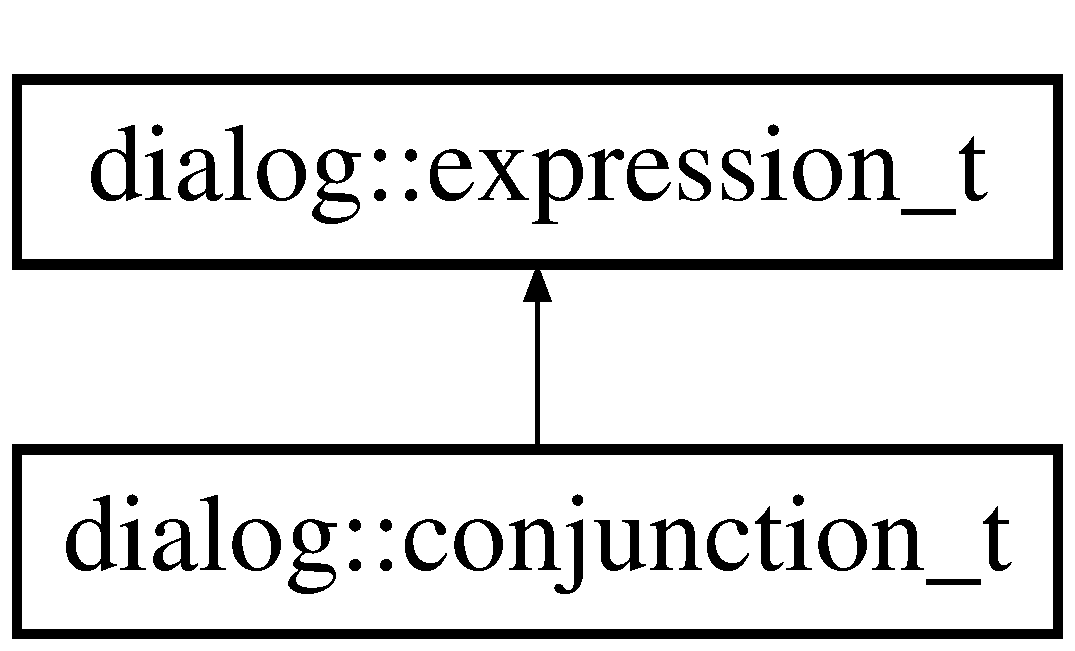
\includegraphics[height=2.000000cm]{structdialog_1_1conjunction__t}
\end{center}
\end{figure}
\subsection*{Public Member Functions}
\begin{DoxyCompactItemize}
\item 
\mbox{\Hypertarget{structdialog_1_1conjunction__t_a6b209e62505e025419b9295d28de0fa3}\label{structdialog_1_1conjunction__t_a6b209e62505e025419b9295d28de0fa3}} 
{\bfseries conjunction\+\_\+t} (\hyperlink{structdialog_1_1expression__t}{expression\+\_\+t} $\ast$l, \hyperlink{structdialog_1_1expression__t}{expression\+\_\+t} $\ast$r)
\end{DoxyCompactItemize}
\subsection*{Public Attributes}
\begin{DoxyCompactItemize}
\item 
\mbox{\Hypertarget{structdialog_1_1conjunction__t_a85ed51a16983ebca8c8d757ee61c9d47}\label{structdialog_1_1conjunction__t_a85ed51a16983ebca8c8d757ee61c9d47}} 
\hyperlink{structdialog_1_1expression__t}{expression\+\_\+t} $\ast$ {\bfseries left}
\item 
\mbox{\Hypertarget{structdialog_1_1conjunction__t_a7ff66bb8e0bcae1c21ed0a241a66db6d}\label{structdialog_1_1conjunction__t_a7ff66bb8e0bcae1c21ed0a241a66db6d}} 
\hyperlink{structdialog_1_1expression__t}{expression\+\_\+t} $\ast$ {\bfseries right}
\end{DoxyCompactItemize}


\subsection{Detailed Description}
Conjunction expression. 

The documentation for this struct was generated from the following file\+:\begin{DoxyCompactItemize}
\item 
/\+Users/neil/\+Documents/\+Berkeley/research/dialog/libdialog/dialog/expression.\+h\end{DoxyCompactItemize}

\hypertarget{classdialog_1_1const__bitmap__array__iterator}{}\section{dialog\+:\+:const\+\_\+bitmap\+\_\+array\+\_\+iterator$<$ bitmap\+\_\+array\+\_\+impl $>$ Class Template Reference}
\label{classdialog_1_1const__bitmap__array__iterator}\index{dialog\+::const\+\_\+bitmap\+\_\+array\+\_\+iterator$<$ bitmap\+\_\+array\+\_\+impl $>$@{dialog\+::const\+\_\+bitmap\+\_\+array\+\_\+iterator$<$ bitmap\+\_\+array\+\_\+impl $>$}}
\subsection*{Public Types}
\begin{DoxyCompactItemize}
\item 
\mbox{\Hypertarget{classdialog_1_1const__bitmap__array__iterator_aea801458a2f710f42ed8b0d9187e3da2}\label{classdialog_1_1const__bitmap__array__iterator_aea801458a2f710f42ed8b0d9187e3da2}} 
typedef bitmap\+\_\+array\+\_\+impl\+::pos\+\_\+type {\bfseries pos\+\_\+type}
\item 
\mbox{\Hypertarget{classdialog_1_1const__bitmap__array__iterator_afd5cfd9700068580567a6e215762488f}\label{classdialog_1_1const__bitmap__array__iterator_afd5cfd9700068580567a6e215762488f}} 
typedef bitmap\+\_\+array\+\_\+impl\+::difference\+\_\+type {\bfseries difference\+\_\+type}
\item 
\mbox{\Hypertarget{classdialog_1_1const__bitmap__array__iterator_a80b195a60fa01aa6d3afcaaab278b3a0}\label{classdialog_1_1const__bitmap__array__iterator_a80b195a60fa01aa6d3afcaaab278b3a0}} 
typedef bitmap\+\_\+array\+\_\+impl\+::value\+\_\+type {\bfseries value\+\_\+type}
\item 
\mbox{\Hypertarget{classdialog_1_1const__bitmap__array__iterator_a50c79fb683611b8029bcf65170ca82f5}\label{classdialog_1_1const__bitmap__array__iterator_a50c79fb683611b8029bcf65170ca82f5}} 
typedef bitmap\+\_\+array\+\_\+impl\+::pointer {\bfseries pointer}
\item 
\mbox{\Hypertarget{classdialog_1_1const__bitmap__array__iterator_ae33f32321e8dd032e6ee540aa5b254e2}\label{classdialog_1_1const__bitmap__array__iterator_ae33f32321e8dd032e6ee540aa5b254e2}} 
typedef bitmap\+\_\+array\+\_\+impl\+::reference {\bfseries reference}
\item 
\mbox{\Hypertarget{classdialog_1_1const__bitmap__array__iterator_a06e9f1b244152e2b72509edc3869f0a3}\label{classdialog_1_1const__bitmap__array__iterator_a06e9f1b244152e2b72509edc3869f0a3}} 
typedef bitmap\+\_\+array\+\_\+impl\+::iterator\+\_\+category {\bfseries iterator\+\_\+category}
\item 
\mbox{\Hypertarget{classdialog_1_1const__bitmap__array__iterator_aa5a7754abd2dfe01104e1898951ea5b0}\label{classdialog_1_1const__bitmap__array__iterator_aa5a7754abd2dfe01104e1898951ea5b0}} 
typedef bitmap\+\_\+array\+\_\+impl\+::value\+\_\+type {\bfseries const\+\_\+reference}
\end{DoxyCompactItemize}
\subsection*{Public Member Functions}
\begin{DoxyCompactItemize}
\item 
\mbox{\Hypertarget{classdialog_1_1const__bitmap__array__iterator_a7075d06f7ecc1451caf6bc6221f9528b}\label{classdialog_1_1const__bitmap__array__iterator_a7075d06f7ecc1451caf6bc6221f9528b}} 
{\bfseries const\+\_\+bitmap\+\_\+array\+\_\+iterator} (const bitmap\+\_\+array\+\_\+impl $\ast$array, pos\+\_\+type pos)
\item 
\mbox{\Hypertarget{classdialog_1_1const__bitmap__array__iterator_aa51fa9055e17992e79dffdb431b2d0ea}\label{classdialog_1_1const__bitmap__array__iterator_aa51fa9055e17992e79dffdb431b2d0ea}} 
const\+\_\+reference {\bfseries operator$\ast$} () const
\item 
\mbox{\Hypertarget{classdialog_1_1const__bitmap__array__iterator_ae9b0bea5c8a23df628954b56a87672cb}\label{classdialog_1_1const__bitmap__array__iterator_ae9b0bea5c8a23df628954b56a87672cb}} 
\hyperlink{classdialog_1_1const__bitmap__array__iterator}{const\+\_\+bitmap\+\_\+array\+\_\+iterator} \& {\bfseries operator++} ()
\item 
\mbox{\Hypertarget{classdialog_1_1const__bitmap__array__iterator_a72ba600427e03a626ee7dc31c20936ff}\label{classdialog_1_1const__bitmap__array__iterator_a72ba600427e03a626ee7dc31c20936ff}} 
\hyperlink{classdialog_1_1const__bitmap__array__iterator}{const\+\_\+bitmap\+\_\+array\+\_\+iterator} {\bfseries operator++} (int)
\item 
\mbox{\Hypertarget{classdialog_1_1const__bitmap__array__iterator_a8c5e46157e5b6e718a082708e5ad0250}\label{classdialog_1_1const__bitmap__array__iterator_a8c5e46157e5b6e718a082708e5ad0250}} 
\hyperlink{classdialog_1_1const__bitmap__array__iterator}{const\+\_\+bitmap\+\_\+array\+\_\+iterator} \& {\bfseries operator-\/-\/} ()
\item 
\mbox{\Hypertarget{classdialog_1_1const__bitmap__array__iterator_a95edb0c5d6e7543ec66c02b7ee06a277}\label{classdialog_1_1const__bitmap__array__iterator_a95edb0c5d6e7543ec66c02b7ee06a277}} 
\hyperlink{classdialog_1_1const__bitmap__array__iterator}{const\+\_\+bitmap\+\_\+array\+\_\+iterator} {\bfseries operator-\/-\/} (int)
\item 
\mbox{\Hypertarget{classdialog_1_1const__bitmap__array__iterator_ab66b6c645e81ea26d7fd5d6992f30b2f}\label{classdialog_1_1const__bitmap__array__iterator_ab66b6c645e81ea26d7fd5d6992f30b2f}} 
\hyperlink{classdialog_1_1const__bitmap__array__iterator}{const\+\_\+bitmap\+\_\+array\+\_\+iterator} \& {\bfseries operator+=} (difference\+\_\+type i)
\item 
\mbox{\Hypertarget{classdialog_1_1const__bitmap__array__iterator_a1bdaf70cbe096ab50397d8381340c427}\label{classdialog_1_1const__bitmap__array__iterator_a1bdaf70cbe096ab50397d8381340c427}} 
\hyperlink{classdialog_1_1const__bitmap__array__iterator}{const\+\_\+bitmap\+\_\+array\+\_\+iterator} \& {\bfseries operator-\/=} (difference\+\_\+type i)
\item 
\mbox{\Hypertarget{classdialog_1_1const__bitmap__array__iterator_a2362728e67714009344a233823597480}\label{classdialog_1_1const__bitmap__array__iterator_a2362728e67714009344a233823597480}} 
\hyperlink{classdialog_1_1const__bitmap__array__iterator}{const\+\_\+bitmap\+\_\+array\+\_\+iterator} {\bfseries operator+} (difference\+\_\+type i) const
\item 
\mbox{\Hypertarget{classdialog_1_1const__bitmap__array__iterator_af03b1c8fc7a9aa15532572d183d0632e}\label{classdialog_1_1const__bitmap__array__iterator_af03b1c8fc7a9aa15532572d183d0632e}} 
\hyperlink{classdialog_1_1const__bitmap__array__iterator}{const\+\_\+bitmap\+\_\+array\+\_\+iterator} {\bfseries operator-\/} (difference\+\_\+type i) const
\item 
\mbox{\Hypertarget{classdialog_1_1const__bitmap__array__iterator_a85aba6ec211b84b3d0bf9df8aa24ab5a}\label{classdialog_1_1const__bitmap__array__iterator_a85aba6ec211b84b3d0bf9df8aa24ab5a}} 
const\+\_\+reference {\bfseries operator\mbox{[}$\,$\mbox{]}} (difference\+\_\+type i) const
\item 
\mbox{\Hypertarget{classdialog_1_1const__bitmap__array__iterator_a61e25a6922678973e248f21137d57b5e}\label{classdialog_1_1const__bitmap__array__iterator_a61e25a6922678973e248f21137d57b5e}} 
bool {\bfseries operator==} (const \hyperlink{classdialog_1_1const__bitmap__array__iterator}{const\+\_\+bitmap\+\_\+array\+\_\+iterator} \&it) const
\item 
\mbox{\Hypertarget{classdialog_1_1const__bitmap__array__iterator_ad0aa8343bb665cbeee8590e8c6171b07}\label{classdialog_1_1const__bitmap__array__iterator_ad0aa8343bb665cbeee8590e8c6171b07}} 
bool {\bfseries operator!=} (const \hyperlink{classdialog_1_1const__bitmap__array__iterator}{const\+\_\+bitmap\+\_\+array\+\_\+iterator} \&it) const
\item 
\mbox{\Hypertarget{classdialog_1_1const__bitmap__array__iterator_aa2181f6280c1d3e51f4fe03a86fc1a57}\label{classdialog_1_1const__bitmap__array__iterator_aa2181f6280c1d3e51f4fe03a86fc1a57}} 
bool {\bfseries operator$<$} (const \hyperlink{classdialog_1_1const__bitmap__array__iterator}{const\+\_\+bitmap\+\_\+array\+\_\+iterator} \&it) const
\item 
\mbox{\Hypertarget{classdialog_1_1const__bitmap__array__iterator_a2fd2de645d4c729a16be22c4c14614d1}\label{classdialog_1_1const__bitmap__array__iterator_a2fd2de645d4c729a16be22c4c14614d1}} 
bool {\bfseries operator$>$} (const \hyperlink{classdialog_1_1const__bitmap__array__iterator}{const\+\_\+bitmap\+\_\+array\+\_\+iterator} \&it) const
\item 
\mbox{\Hypertarget{classdialog_1_1const__bitmap__array__iterator_a3e31bbc2c3f06e1fd7856440ad8ae693}\label{classdialog_1_1const__bitmap__array__iterator_a3e31bbc2c3f06e1fd7856440ad8ae693}} 
bool {\bfseries operator$>$=} (const \hyperlink{classdialog_1_1const__bitmap__array__iterator}{const\+\_\+bitmap\+\_\+array\+\_\+iterator} \&it) const
\item 
\mbox{\Hypertarget{classdialog_1_1const__bitmap__array__iterator_a64755d66edcdc3d3fa35a2749c276200}\label{classdialog_1_1const__bitmap__array__iterator_a64755d66edcdc3d3fa35a2749c276200}} 
bool {\bfseries operator$<$=} (const \hyperlink{classdialog_1_1const__bitmap__array__iterator}{const\+\_\+bitmap\+\_\+array\+\_\+iterator} \&it) const
\item 
\mbox{\Hypertarget{classdialog_1_1const__bitmap__array__iterator_a25f00aa8a3574b35138979901eb4121d}\label{classdialog_1_1const__bitmap__array__iterator_a25f00aa8a3574b35138979901eb4121d}} 
difference\+\_\+type {\bfseries operator-\/} (const \hyperlink{classdialog_1_1const__bitmap__array__iterator}{const\+\_\+bitmap\+\_\+array\+\_\+iterator} \&it)
\end{DoxyCompactItemize}


The documentation for this class was generated from the following file\+:\begin{DoxyCompactItemize}
\item 
/\+Users/neil/\+Documents/\+Berkeley/research/dialog/libdialog/dialog/bitmap\+\_\+array.\+h\end{DoxyCompactItemize}

\hypertarget{classdialog_1_1constants}{}\section{dialog\+:\+:constants Class Reference}
\label{classdialog_1_1constants}\index{dialog\+::constants@{dialog\+::constants}}
\subsection*{Static Public Attributes}
\begin{DoxyCompactItemize}
\item 
\mbox{\Hypertarget{classdialog_1_1constants_aaa85f1a9924be4abd5cc4a54714ee115}\label{classdialog_1_1constants_aaa85f1a9924be4abd5cc4a54714ee115}} 
static const int {\bfseries H\+A\+R\+D\+W\+A\+R\+E\+\_\+\+C\+O\+N\+C\+U\+R\+R\+E\+N\+CY} = std\+::thread\+::hardware\+\_\+concurrency()
\item 
\mbox{\Hypertarget{classdialog_1_1constants_a4f7aa966b00a011b90ff6ad7b4455f6d}\label{classdialog_1_1constants_a4f7aa966b00a011b90ff6ad7b4455f6d}} 
static constexpr double {\bfseries D\+E\+F\+A\+U\+L\+T\+\_\+\+I\+N\+D\+E\+X\+\_\+\+B\+U\+C\+K\+E\+T\+\_\+\+S\+I\+ZE} = 1.\+0
\item 
\mbox{\Hypertarget{classdialog_1_1constants_aeb655030eb65804ef504b2ab7f781ba6}\label{classdialog_1_1constants_aeb655030eb65804ef504b2ab7f781ba6}} 
static constexpr uint64\+\_\+t {\bfseries D\+E\+F\+A\+U\+L\+T\+\_\+\+T\+I\+M\+E\+\_\+\+R\+E\+S\+O\+L\+U\+T\+I\+O\+N\+\_\+\+NS} = 1e6
\item 
\mbox{\Hypertarget{classdialog_1_1constants_a6397aad130172a714ab62eaa38eccd8c}\label{classdialog_1_1constants_a6397aad130172a714ab62eaa38eccd8c}} 
static constexpr uint64\+\_\+t {\bfseries D\+E\+F\+A\+U\+L\+T\+\_\+\+M\+O\+N\+I\+T\+O\+R\+\_\+\+W\+I\+N\+D\+O\+W\+\_\+\+MS} = 10
\item 
\mbox{\Hypertarget{classdialog_1_1constants_ac7adb4a95712cea788f3e6d8684a347d}\label{classdialog_1_1constants_ac7adb4a95712cea788f3e6d8684a347d}} 
static constexpr uint64\+\_\+t {\bfseries D\+E\+F\+A\+U\+L\+T\+\_\+\+M\+O\+N\+I\+T\+O\+R\+\_\+\+P\+E\+R\+I\+O\+D\+I\+C\+I\+T\+Y\+\_\+\+MS} = 1
\end{DoxyCompactItemize}


The documentation for this class was generated from the following file\+:\begin{DoxyCompactItemize}
\item 
/\+Users/neil/\+Documents/\+Berkeley/research/dialog/libdialog/dialog/constants.\+h\end{DoxyCompactItemize}

\hypertarget{structdialog_1_1data}{}\section{dialog\+:\+:data Struct Reference}
\label{structdialog_1_1data}\index{dialog\+::data@{dialog\+::data}}
\subsection*{Public Member Functions}
\begin{DoxyCompactItemize}
\item 
\mbox{\Hypertarget{structdialog_1_1data_a67f95b3c190f4a2a990daff1fb6bf53c}\label{structdialog_1_1data_a67f95b3c190f4a2a990daff1fb6bf53c}} 
{\bfseries data} (const void $\ast$\+\_\+ptr, size\+\_\+t \+\_\+size)
\item 
\mbox{\Hypertarget{structdialog_1_1data_a805239f9c1a7a87f33db10f42c036982}\label{structdialog_1_1data_a805239f9c1a7a87f33db10f42c036982}} 
{\footnotesize template$<$typename T $>$ }\\T {\bfseries as} () const
\end{DoxyCompactItemize}
\subsection*{Public Attributes}
\begin{DoxyCompactItemize}
\item 
\mbox{\Hypertarget{structdialog_1_1data_aae8687e0660a1d3dd5ec1b6555b70c25}\label{structdialog_1_1data_aae8687e0660a1d3dd5ec1b6555b70c25}} 
const void $\ast$ {\bfseries ptr}
\item 
\mbox{\Hypertarget{structdialog_1_1data_a44a7d81b5ae71a723cdfaa1dffb9d1e4}\label{structdialog_1_1data_a44a7d81b5ae71a723cdfaa1dffb9d1e4}} 
size\+\_\+t {\bfseries size}
\end{DoxyCompactItemize}


The documentation for this struct was generated from the following file\+:\begin{DoxyCompactItemize}
\item 
/\+Users/neil/\+Documents/\+Berkeley/research/dialog/libdialog/dialog/data.\+h\end{DoxyCompactItemize}

\hypertarget{structdialog_1_1data__type}{}\section{dialog\+:\+:data\+\_\+type Struct Reference}
\label{structdialog_1_1data__type}\index{dialog\+::data\+\_\+type@{dialog\+::data\+\_\+type}}
\subsection*{Public Member Functions}
\begin{DoxyCompactItemize}
\item 
\mbox{\Hypertarget{structdialog_1_1data__type_acfccb37a96a912023a361474d0a91886}\label{structdialog_1_1data__type_acfccb37a96a912023a361474d0a91886}} 
{\bfseries data\+\_\+type} (type\+\_\+id \+\_\+id=type\+\_\+id\+::\+D\+\_\+\+N\+O\+NE, size\+\_\+t \+\_\+size=0)
\item 
\mbox{\Hypertarget{structdialog_1_1data__type_a52915d9d5b5f170250104b907ebfd3aa}\label{structdialog_1_1data__type_a52915d9d5b5f170250104b907ebfd3aa}} 
void $\ast$ {\bfseries min} () const
\item 
\mbox{\Hypertarget{structdialog_1_1data__type_a5a36e3b7eab5a53b462c8186ffb14413}\label{structdialog_1_1data__type_a5a36e3b7eab5a53b462c8186ffb14413}} 
void $\ast$ {\bfseries max} () const
\item 
\mbox{\Hypertarget{structdialog_1_1data__type_a1fb5308cb864cc1c6de1890bb76683f3}\label{structdialog_1_1data__type_a1fb5308cb864cc1c6de1890bb76683f3}} 
void $\ast$ {\bfseries one} () const
\item 
\mbox{\Hypertarget{structdialog_1_1data__type_afc18fbb61b17d9f2d436e5e91a16be63}\label{structdialog_1_1data__type_afc18fbb61b17d9f2d436e5e91a16be63}} 
void $\ast$ {\bfseries zero} () const
\item 
\mbox{\Hypertarget{structdialog_1_1data__type_a4f1f9514f927ccef44d0326ed8108f6c}\label{structdialog_1_1data__type_a4f1f9514f927ccef44d0326ed8108f6c}} 
\hyperlink{structdialog_1_1data__type}{data\+\_\+type} \& {\bfseries operator=} (const \hyperlink{structdialog_1_1data__type}{data\+\_\+type} \&other)
\item 
\mbox{\Hypertarget{structdialog_1_1data__type_a8af26c0fb43a080dda1d08772b3c1c4d}\label{structdialog_1_1data__type_a8af26c0fb43a080dda1d08772b3c1c4d}} 
bool {\bfseries operator==} (const \hyperlink{structdialog_1_1data__type}{data\+\_\+type} \&other) const
\item 
\mbox{\Hypertarget{structdialog_1_1data__type_a39f84bb75dfe8a227015fa2735fe8d42}\label{structdialog_1_1data__type_a39f84bb75dfe8a227015fa2735fe8d42}} 
bool {\bfseries operator!=} (const \hyperlink{structdialog_1_1data__type}{data\+\_\+type} \&other) const
\item 
\mbox{\Hypertarget{structdialog_1_1data__type_aba8aaca842503e3b0118825520070988}\label{structdialog_1_1data__type_aba8aaca842503e3b0118825520070988}} 
const relational\+\_\+fn \& {\bfseries relop} (relop\+\_\+id rid) const
\item 
\mbox{\Hypertarget{structdialog_1_1data__type_aa4307e017509255887d8ddf25358c16c}\label{structdialog_1_1data__type_aa4307e017509255887d8ddf25358c16c}} 
const unary\+\_\+fn \& {\bfseries unaryop} (unaryop\+\_\+id uid) const
\item 
\mbox{\Hypertarget{structdialog_1_1data__type_a27657c80d0951a937be61d199fabff7f}\label{structdialog_1_1data__type_a27657c80d0951a937be61d199fabff7f}} 
const binary\+\_\+fn \& {\bfseries binaryop} (binaryop\+\_\+id bid) const
\item 
\mbox{\Hypertarget{structdialog_1_1data__type_ac1c63786702a0c2f4fe7367c34f3880a}\label{structdialog_1_1data__type_ac1c63786702a0c2f4fe7367c34f3880a}} 
const key\+\_\+op \& {\bfseries keytransform} () const
\item 
\mbox{\Hypertarget{structdialog_1_1data__type_a5f32bdf7dd0dbceb45727672810cfd3f}\label{structdialog_1_1data__type_a5f32bdf7dd0dbceb45727672810cfd3f}} 
std\+::string {\bfseries to\+\_\+string} () const
\end{DoxyCompactItemize}
\subsection*{Public Attributes}
\begin{DoxyCompactItemize}
\item 
\mbox{\Hypertarget{structdialog_1_1data__type_afe64e30abff6e7d1488dc8ef5a911df6}\label{structdialog_1_1data__type_afe64e30abff6e7d1488dc8ef5a911df6}} 
type\+\_\+id {\bfseries id}
\item 
\mbox{\Hypertarget{structdialog_1_1data__type_a9587af728278c26fb62eb25a0988354b}\label{structdialog_1_1data__type_a9587af728278c26fb62eb25a0988354b}} 
size\+\_\+t {\bfseries size}
\end{DoxyCompactItemize}


The documentation for this struct was generated from the following file\+:\begin{DoxyCompactItemize}
\item 
/\+Users/neil/\+Documents/\+Berkeley/research/dialog/libdialog/dialog/data\+\_\+types.\+h\end{DoxyCompactItemize}

\hypertarget{classdialog_1_1delta__encoded__array}{}\section{dialog\+:\+:delta\+\_\+encoded\+\_\+array$<$ T, sampling\+\_\+rate $>$ Class Template Reference}
\label{classdialog_1_1delta__encoded__array}\index{dialog\+::delta\+\_\+encoded\+\_\+array$<$ T, sampling\+\_\+rate $>$@{dialog\+::delta\+\_\+encoded\+\_\+array$<$ T, sampling\+\_\+rate $>$}}
Inheritance diagram for dialog\+:\+:delta\+\_\+encoded\+\_\+array$<$ T, sampling\+\_\+rate $>$\+:\begin{figure}[H]
\begin{center}
\leavevmode
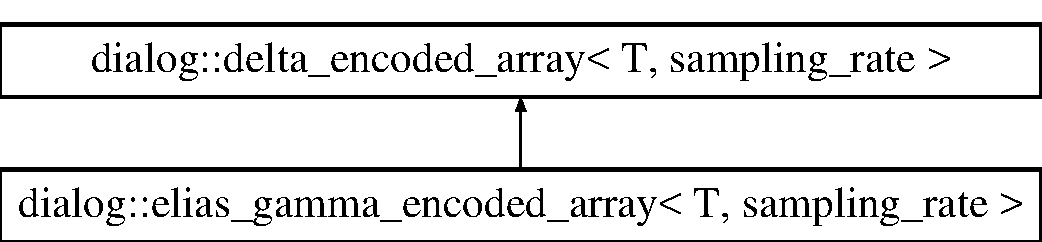
\includegraphics[height=2.000000cm]{classdialog_1_1delta__encoded__array}
\end{center}
\end{figure}
\subsection*{Public Types}
\begin{DoxyCompactItemize}
\item 
\mbox{\Hypertarget{classdialog_1_1delta__encoded__array_a0cd3b42e267ec14eeb48f76bf3211c8f}\label{classdialog_1_1delta__encoded__array_a0cd3b42e267ec14eeb48f76bf3211c8f}} 
typedef size\+\_\+t {\bfseries size\+\_\+type}
\item 
\mbox{\Hypertarget{classdialog_1_1delta__encoded__array_a9ed959d0d2070fa3044847cf4c3bbc12}\label{classdialog_1_1delta__encoded__array_a9ed959d0d2070fa3044847cf4c3bbc12}} 
typedef size\+\_\+t {\bfseries pos\+\_\+type}
\item 
\mbox{\Hypertarget{classdialog_1_1delta__encoded__array_aaa88ddf82d3790ea40350b14931c515e}\label{classdialog_1_1delta__encoded__array_aaa88ddf82d3790ea40350b14931c515e}} 
typedef uint8\+\_\+t {\bfseries width\+\_\+type}
\end{DoxyCompactItemize}
\subsection*{Public Member Functions}
\begin{DoxyCompactItemize}
\item 
\hyperlink{classdialog_1_1delta__encoded__array_a3b5f62d85c360a2ac4bc30db2b790d8d}{delta\+\_\+encoded\+\_\+array} ()
\item 
virtual \hyperlink{classdialog_1_1delta__encoded__array_acdf15405bdd9cebcbe8de93a797516cb}{$\sim$delta\+\_\+encoded\+\_\+array} ()
\item 
virtual size\+\_\+type \hyperlink{classdialog_1_1delta__encoded__array_a533eeb8833bb554513c86eb7f1ce635f}{serialize} (std\+::ostream \&out)
\item 
virtual size\+\_\+type \hyperlink{classdialog_1_1delta__encoded__array_aced4bc1f11a264fe3263b89be0e55d33}{deserialize} (std\+::istream \&in)
\end{DoxyCompactItemize}
\subsection*{Protected Member Functions}
\begin{DoxyCompactItemize}
\item 
virtual width\+\_\+type \hyperlink{classdialog_1_1delta__encoded__array_a5a7dd4499765ed12a030b25ca3452ea3}{encoding\+\_\+size} (T delta)=0
\item 
virtual void \hyperlink{classdialog_1_1delta__encoded__array_a4ad7e0110c90c91684873f40c778cd6e}{encode\+\_\+deltas} (T $\ast$deltas, size\+\_\+type num\+\_\+deltas)=0
\item 
void \hyperlink{classdialog_1_1delta__encoded__array_aaab973ffb4fa2d62fb658e5dbcc0acad}{encode} (T $\ast$elements, size\+\_\+type num\+\_\+elements)
\end{DoxyCompactItemize}
\subsection*{Protected Attributes}
\begin{DoxyCompactItemize}
\item 
\mbox{\Hypertarget{classdialog_1_1delta__encoded__array_af92d09ac19d1c6ac9f9271b0fc857404}\label{classdialog_1_1delta__encoded__array_af92d09ac19d1c6ac9f9271b0fc857404}} 
\hyperlink{classdialog_1_1unsized__bitmap__array}{unsized\+\_\+bitmap\+\_\+array}$<$ T $>$ $\ast$ {\bfseries samples\+\_\+}
\item 
\mbox{\Hypertarget{classdialog_1_1delta__encoded__array_ad2ca110a0d18668bc6503effd89eb8a8}\label{classdialog_1_1delta__encoded__array_ad2ca110a0d18668bc6503effd89eb8a8}} 
\hyperlink{classdialog_1_1unsized__bitmap__array}{unsized\+\_\+bitmap\+\_\+array}$<$ pos\+\_\+type $>$ $\ast$ {\bfseries delta\+\_\+offsets\+\_\+}
\item 
\mbox{\Hypertarget{classdialog_1_1delta__encoded__array_ab1b64295148db2954a85757aad6865cf}\label{classdialog_1_1delta__encoded__array_ab1b64295148db2954a85757aad6865cf}} 
\hyperlink{classdialog_1_1bitmap}{bitmap} $\ast$ {\bfseries deltas\+\_\+}
\end{DoxyCompactItemize}


\subsection{Constructor \& Destructor Documentation}
\mbox{\Hypertarget{classdialog_1_1delta__encoded__array_a3b5f62d85c360a2ac4bc30db2b790d8d}\label{classdialog_1_1delta__encoded__array_a3b5f62d85c360a2ac4bc30db2b790d8d}} 
\index{dialog\+::delta\+\_\+encoded\+\_\+array@{dialog\+::delta\+\_\+encoded\+\_\+array}!delta\+\_\+encoded\+\_\+array@{delta\+\_\+encoded\+\_\+array}}
\index{delta\+\_\+encoded\+\_\+array@{delta\+\_\+encoded\+\_\+array}!dialog\+::delta\+\_\+encoded\+\_\+array@{dialog\+::delta\+\_\+encoded\+\_\+array}}
\subsubsection{\texorpdfstring{delta\+\_\+encoded\+\_\+array()}{delta\_encoded\_array()}}
{\footnotesize\ttfamily template$<$typename T, uint32\+\_\+t sampling\+\_\+rate = 128$>$ \\
\hyperlink{classdialog_1_1delta__encoded__array}{dialog\+::delta\+\_\+encoded\+\_\+array}$<$ T, sampling\+\_\+rate $>$\+::\hyperlink{classdialog_1_1delta__encoded__array}{delta\+\_\+encoded\+\_\+array} (\begin{DoxyParamCaption}{ }\end{DoxyParamCaption})\hspace{0.3cm}{\ttfamily [inline]}}

Default constructor that initializes everything to default values \mbox{\Hypertarget{classdialog_1_1delta__encoded__array_acdf15405bdd9cebcbe8de93a797516cb}\label{classdialog_1_1delta__encoded__array_acdf15405bdd9cebcbe8de93a797516cb}} 
\index{dialog\+::delta\+\_\+encoded\+\_\+array@{dialog\+::delta\+\_\+encoded\+\_\+array}!````~delta\+\_\+encoded\+\_\+array@{$\sim$delta\+\_\+encoded\+\_\+array}}
\index{````~delta\+\_\+encoded\+\_\+array@{$\sim$delta\+\_\+encoded\+\_\+array}!dialog\+::delta\+\_\+encoded\+\_\+array@{dialog\+::delta\+\_\+encoded\+\_\+array}}
\subsubsection{\texorpdfstring{$\sim$delta\+\_\+encoded\+\_\+array()}{~delta\_encoded\_array()}}
{\footnotesize\ttfamily template$<$typename T, uint32\+\_\+t sampling\+\_\+rate = 128$>$ \\
virtual \hyperlink{classdialog_1_1delta__encoded__array}{dialog\+::delta\+\_\+encoded\+\_\+array}$<$ T, sampling\+\_\+rate $>$\+::$\sim$\hyperlink{classdialog_1_1delta__encoded__array}{delta\+\_\+encoded\+\_\+array} (\begin{DoxyParamCaption}{ }\end{DoxyParamCaption})\hspace{0.3cm}{\ttfamily [inline]}, {\ttfamily [virtual]}}

Default destructor that deletes all of the samples, offsets, and deltas 

\subsection{Member Function Documentation}
\mbox{\Hypertarget{classdialog_1_1delta__encoded__array_aced4bc1f11a264fe3263b89be0e55d33}\label{classdialog_1_1delta__encoded__array_aced4bc1f11a264fe3263b89be0e55d33}} 
\index{dialog\+::delta\+\_\+encoded\+\_\+array@{dialog\+::delta\+\_\+encoded\+\_\+array}!deserialize@{deserialize}}
\index{deserialize@{deserialize}!dialog\+::delta\+\_\+encoded\+\_\+array@{dialog\+::delta\+\_\+encoded\+\_\+array}}
\subsubsection{\texorpdfstring{deserialize()}{deserialize()}}
{\footnotesize\ttfamily template$<$typename T, uint32\+\_\+t sampling\+\_\+rate = 128$>$ \\
virtual size\+\_\+type \hyperlink{classdialog_1_1delta__encoded__array}{dialog\+::delta\+\_\+encoded\+\_\+array}$<$ T, sampling\+\_\+rate $>$\+::deserialize (\begin{DoxyParamCaption}\item[{std\+::istream \&}]{in }\end{DoxyParamCaption})\hspace{0.3cm}{\ttfamily [inline]}, {\ttfamily [virtual]}}

Deserializes input stream to an array 
\begin{DoxyParams}{Parameters}
{\em in} & The input stream \\
\hline
\end{DoxyParams}
\begin{DoxyReturn}{Returns}
The size of the array from the input stream 
\end{DoxyReturn}
\mbox{\Hypertarget{classdialog_1_1delta__encoded__array_aaab973ffb4fa2d62fb658e5dbcc0acad}\label{classdialog_1_1delta__encoded__array_aaab973ffb4fa2d62fb658e5dbcc0acad}} 
\index{dialog\+::delta\+\_\+encoded\+\_\+array@{dialog\+::delta\+\_\+encoded\+\_\+array}!encode@{encode}}
\index{encode@{encode}!dialog\+::delta\+\_\+encoded\+\_\+array@{dialog\+::delta\+\_\+encoded\+\_\+array}}
\subsubsection{\texorpdfstring{encode()}{encode()}}
{\footnotesize\ttfamily template$<$typename T, uint32\+\_\+t sampling\+\_\+rate = 128$>$ \\
void \hyperlink{classdialog_1_1delta__encoded__array}{dialog\+::delta\+\_\+encoded\+\_\+array}$<$ T, sampling\+\_\+rate $>$\+::encode (\begin{DoxyParamCaption}\item[{T $\ast$}]{elements,  }\item[{size\+\_\+type}]{num\+\_\+elements }\end{DoxyParamCaption})\hspace{0.3cm}{\ttfamily [inline]}, {\ttfamily [protected]}}

Encode the delta encoded array 
\begin{DoxyParams}{Parameters}
{\em elements} & The elements of the array \\
\hline
{\em num\+\_\+elements} & The number of elements \\
\hline
\end{DoxyParams}
\mbox{\Hypertarget{classdialog_1_1delta__encoded__array_a4ad7e0110c90c91684873f40c778cd6e}\label{classdialog_1_1delta__encoded__array_a4ad7e0110c90c91684873f40c778cd6e}} 
\index{dialog\+::delta\+\_\+encoded\+\_\+array@{dialog\+::delta\+\_\+encoded\+\_\+array}!encode\+\_\+deltas@{encode\+\_\+deltas}}
\index{encode\+\_\+deltas@{encode\+\_\+deltas}!dialog\+::delta\+\_\+encoded\+\_\+array@{dialog\+::delta\+\_\+encoded\+\_\+array}}
\subsubsection{\texorpdfstring{encode\+\_\+deltas()}{encode\_deltas()}}
{\footnotesize\ttfamily template$<$typename T, uint32\+\_\+t sampling\+\_\+rate = 128$>$ \\
virtual void \hyperlink{classdialog_1_1delta__encoded__array}{dialog\+::delta\+\_\+encoded\+\_\+array}$<$ T, sampling\+\_\+rate $>$\+::encode\+\_\+deltas (\begin{DoxyParamCaption}\item[{T $\ast$}]{deltas,  }\item[{size\+\_\+type}]{num\+\_\+deltas }\end{DoxyParamCaption})\hspace{0.3cm}{\ttfamily [protected]}, {\ttfamily [pure virtual]}}

Encode the delta values 
\begin{DoxyParams}{Parameters}
{\em deltas} & The delta values \\
\hline
{\em num\+\_\+deltas} & The number of deltas \\
\hline
\end{DoxyParams}
\mbox{\Hypertarget{classdialog_1_1delta__encoded__array_a5a7dd4499765ed12a030b25ca3452ea3}\label{classdialog_1_1delta__encoded__array_a5a7dd4499765ed12a030b25ca3452ea3}} 
\index{dialog\+::delta\+\_\+encoded\+\_\+array@{dialog\+::delta\+\_\+encoded\+\_\+array}!encoding\+\_\+size@{encoding\+\_\+size}}
\index{encoding\+\_\+size@{encoding\+\_\+size}!dialog\+::delta\+\_\+encoded\+\_\+array@{dialog\+::delta\+\_\+encoded\+\_\+array}}
\subsubsection{\texorpdfstring{encoding\+\_\+size()}{encoding\_size()}}
{\footnotesize\ttfamily template$<$typename T, uint32\+\_\+t sampling\+\_\+rate = 128$>$ \\
virtual width\+\_\+type \hyperlink{classdialog_1_1delta__encoded__array}{dialog\+::delta\+\_\+encoded\+\_\+array}$<$ T, sampling\+\_\+rate $>$\+::encoding\+\_\+size (\begin{DoxyParamCaption}\item[{T}]{delta }\end{DoxyParamCaption})\hspace{0.3cm}{\ttfamily [protected]}, {\ttfamily [pure virtual]}}

Get the encoding size for an delta value 
\begin{DoxyParams}{Parameters}
{\em delta} & The delta value \\
\hline
\end{DoxyParams}
\begin{DoxyReturn}{Returns}
The width type of the delta 
\end{DoxyReturn}
\mbox{\Hypertarget{classdialog_1_1delta__encoded__array_a533eeb8833bb554513c86eb7f1ce635f}\label{classdialog_1_1delta__encoded__array_a533eeb8833bb554513c86eb7f1ce635f}} 
\index{dialog\+::delta\+\_\+encoded\+\_\+array@{dialog\+::delta\+\_\+encoded\+\_\+array}!serialize@{serialize}}
\index{serialize@{serialize}!dialog\+::delta\+\_\+encoded\+\_\+array@{dialog\+::delta\+\_\+encoded\+\_\+array}}
\subsubsection{\texorpdfstring{serialize()}{serialize()}}
{\footnotesize\ttfamily template$<$typename T, uint32\+\_\+t sampling\+\_\+rate = 128$>$ \\
virtual size\+\_\+type \hyperlink{classdialog_1_1delta__encoded__array}{dialog\+::delta\+\_\+encoded\+\_\+array}$<$ T, sampling\+\_\+rate $>$\+::serialize (\begin{DoxyParamCaption}\item[{std\+::ostream \&}]{out }\end{DoxyParamCaption})\hspace{0.3cm}{\ttfamily [inline]}, {\ttfamily [virtual]}}

Serializes array to output stream 
\begin{DoxyParams}{Parameters}
{\em out} & The output stream \\
\hline
\end{DoxyParams}
\begin{DoxyReturn}{Returns}
The size of the data in the output stream 
\end{DoxyReturn}


The documentation for this class was generated from the following file\+:\begin{DoxyCompactItemize}
\item 
/\+Users/neil/\+Documents/\+Berkeley/research/dialog/libdialog/dialog/delta\+\_\+encoded\+\_\+array.\+h\end{DoxyCompactItemize}

\hypertarget{classdialog_1_1dialog__store}{}\section{dialog\+:\+:dialog\+\_\+store Class Reference}
\label{classdialog_1_1dialog__store}\index{dialog\+::dialog\+\_\+store@{dialog\+::dialog\+\_\+store}}
\subsection*{Public Member Functions}
\begin{DoxyCompactItemize}
\item 
\hyperlink{classdialog_1_1dialog__store_a88dd772873fbd8c51bb21baa7302ebee}{dialog\+\_\+store} (const std\+::string \&data\+\_\+path)
\item 
int64\+\_\+t \hyperlink{classdialog_1_1dialog__store_aec46cdcce3866d0840cf01528eb5e6c0}{add\+\_\+table} (const std\+::string \&table\+\_\+name, const std\+::vector$<$ \hyperlink{classdialog_1_1column__t}{column\+\_\+t} $>$ \&schema, const storage\+::storage\+\_\+id id)
\item 
int64\+\_\+t \hyperlink{classdialog_1_1dialog__store_a749d49076f2107e32b65be5d79d5781c}{get\+\_\+table\+\_\+id} (const std\+::string \&table\+\_\+name) const
\item 
\hyperlink{classdialog_1_1dialog__table}{dialog\+\_\+table} $\ast$ \hyperlink{classdialog_1_1dialog__store_a3d951f8e4bc697af2fdd7b9f225453d8}{get\+\_\+table} (const std\+::string \&table\+\_\+name)
\item 
\hyperlink{classdialog_1_1dialog__table}{dialog\+\_\+table} $\ast$ \hyperlink{classdialog_1_1dialog__store_a7fb7214a8098e54fd3d2ac0bfae4a431}{get\+\_\+table} (int64\+\_\+t table\+\_\+id)
\item 
int64\+\_\+t \hyperlink{classdialog_1_1dialog__store_a15b6b065d529ede947ff3ca4db77ab56}{remove\+\_\+table} (const std\+::string \&table\+\_\+name)
\item 
int64\+\_\+t \hyperlink{classdialog_1_1dialog__store_a7557cfcb6f7f5458031b7b3971d9d7cd}{remove\+\_\+table} (int64\+\_\+t table\+\_\+id)
\end{DoxyCompactItemize}


\subsection{Constructor \& Destructor Documentation}
\mbox{\Hypertarget{classdialog_1_1dialog__store_a88dd772873fbd8c51bb21baa7302ebee}\label{classdialog_1_1dialog__store_a88dd772873fbd8c51bb21baa7302ebee}} 
\index{dialog\+::dialog\+\_\+store@{dialog\+::dialog\+\_\+store}!dialog\+\_\+store@{dialog\+\_\+store}}
\index{dialog\+\_\+store@{dialog\+\_\+store}!dialog\+::dialog\+\_\+store@{dialog\+::dialog\+\_\+store}}
\subsubsection{\texorpdfstring{dialog\+\_\+store()}{dialog\_store()}}
{\footnotesize\ttfamily dialog\+::dialog\+\_\+store\+::dialog\+\_\+store (\begin{DoxyParamCaption}\item[{const std\+::string \&}]{data\+\_\+path }\end{DoxyParamCaption})\hspace{0.3cm}{\ttfamily [inline]}}

Constructor for creating dialog store 
\begin{DoxyParams}{Parameters}
{\em data\+\_\+path} & The data path for the store \\
\hline
\end{DoxyParams}


\subsection{Member Function Documentation}
\mbox{\Hypertarget{classdialog_1_1dialog__store_aec46cdcce3866d0840cf01528eb5e6c0}\label{classdialog_1_1dialog__store_aec46cdcce3866d0840cf01528eb5e6c0}} 
\index{dialog\+::dialog\+\_\+store@{dialog\+::dialog\+\_\+store}!add\+\_\+table@{add\+\_\+table}}
\index{add\+\_\+table@{add\+\_\+table}!dialog\+::dialog\+\_\+store@{dialog\+::dialog\+\_\+store}}
\subsubsection{\texorpdfstring{add\+\_\+table()}{add\_table()}}
{\footnotesize\ttfamily int64\+\_\+t dialog\+::dialog\+\_\+store\+::add\+\_\+table (\begin{DoxyParamCaption}\item[{const std\+::string \&}]{table\+\_\+name,  }\item[{const std\+::vector$<$ \hyperlink{classdialog_1_1column__t}{column\+\_\+t} $>$ \&}]{schema,  }\item[{const storage\+::storage\+\_\+id}]{id }\end{DoxyParamCaption})\hspace{0.3cm}{\ttfamily [inline]}}

Adds a table to the dialog store 
\begin{DoxyParams}{Parameters}
{\em table\+\_\+name} & The name of the table \\
\hline
{\em schema} & List of columns that define the schema \\
\hline
{\em id} & The ide of the store \\
\hline
\end{DoxyParams}
\begin{DoxyReturn}{Returns}
The id of the table 
\end{DoxyReturn}
\mbox{\Hypertarget{classdialog_1_1dialog__store_a3d951f8e4bc697af2fdd7b9f225453d8}\label{classdialog_1_1dialog__store_a3d951f8e4bc697af2fdd7b9f225453d8}} 
\index{dialog\+::dialog\+\_\+store@{dialog\+::dialog\+\_\+store}!get\+\_\+table@{get\+\_\+table}}
\index{get\+\_\+table@{get\+\_\+table}!dialog\+::dialog\+\_\+store@{dialog\+::dialog\+\_\+store}}
\subsubsection{\texorpdfstring{get\+\_\+table()}{get\_table()}\hspace{0.1cm}{\footnotesize\ttfamily [1/2]}}
{\footnotesize\ttfamily \hyperlink{classdialog_1_1dialog__table}{dialog\+\_\+table}$\ast$ dialog\+::dialog\+\_\+store\+::get\+\_\+table (\begin{DoxyParamCaption}\item[{const std\+::string \&}]{table\+\_\+name }\end{DoxyParamCaption})\hspace{0.3cm}{\ttfamily [inline]}}

Gets the specified table 
\begin{DoxyParams}{Parameters}
{\em table\+\_\+name} & The name of the table \\
\hline
\end{DoxyParams}
\begin{DoxyReturn}{Returns}
The table that matches the table name 
\end{DoxyReturn}
\mbox{\Hypertarget{classdialog_1_1dialog__store_a7fb7214a8098e54fd3d2ac0bfae4a431}\label{classdialog_1_1dialog__store_a7fb7214a8098e54fd3d2ac0bfae4a431}} 
\index{dialog\+::dialog\+\_\+store@{dialog\+::dialog\+\_\+store}!get\+\_\+table@{get\+\_\+table}}
\index{get\+\_\+table@{get\+\_\+table}!dialog\+::dialog\+\_\+store@{dialog\+::dialog\+\_\+store}}
\subsubsection{\texorpdfstring{get\+\_\+table()}{get\_table()}\hspace{0.1cm}{\footnotesize\ttfamily [2/2]}}
{\footnotesize\ttfamily \hyperlink{classdialog_1_1dialog__table}{dialog\+\_\+table}$\ast$ dialog\+::dialog\+\_\+store\+::get\+\_\+table (\begin{DoxyParamCaption}\item[{int64\+\_\+t}]{table\+\_\+id }\end{DoxyParamCaption})\hspace{0.3cm}{\ttfamily [inline]}}

Gets the specified table by id 
\begin{DoxyParams}{Parameters}
{\em table\+\_\+id} & The id of the table \\
\hline
\end{DoxyParams}
\begin{DoxyReturn}{Returns}
The table that matches the id 
\end{DoxyReturn}
\mbox{\Hypertarget{classdialog_1_1dialog__store_a749d49076f2107e32b65be5d79d5781c}\label{classdialog_1_1dialog__store_a749d49076f2107e32b65be5d79d5781c}} 
\index{dialog\+::dialog\+\_\+store@{dialog\+::dialog\+\_\+store}!get\+\_\+table\+\_\+id@{get\+\_\+table\+\_\+id}}
\index{get\+\_\+table\+\_\+id@{get\+\_\+table\+\_\+id}!dialog\+::dialog\+\_\+store@{dialog\+::dialog\+\_\+store}}
\subsubsection{\texorpdfstring{get\+\_\+table\+\_\+id()}{get\_table\_id()}}
{\footnotesize\ttfamily int64\+\_\+t dialog\+::dialog\+\_\+store\+::get\+\_\+table\+\_\+id (\begin{DoxyParamCaption}\item[{const std\+::string \&}]{table\+\_\+name }\end{DoxyParamCaption}) const\hspace{0.3cm}{\ttfamily [inline]}}

Gets the id of the table 
\begin{DoxyParams}{Parameters}
{\em table\+\_\+name} & The name of the table \\
\hline
\end{DoxyParams}
\begin{DoxyReturn}{Returns}
The id of the table 
\end{DoxyReturn}
\mbox{\Hypertarget{classdialog_1_1dialog__store_a15b6b065d529ede947ff3ca4db77ab56}\label{classdialog_1_1dialog__store_a15b6b065d529ede947ff3ca4db77ab56}} 
\index{dialog\+::dialog\+\_\+store@{dialog\+::dialog\+\_\+store}!remove\+\_\+table@{remove\+\_\+table}}
\index{remove\+\_\+table@{remove\+\_\+table}!dialog\+::dialog\+\_\+store@{dialog\+::dialog\+\_\+store}}
\subsubsection{\texorpdfstring{remove\+\_\+table()}{remove\_table()}\hspace{0.1cm}{\footnotesize\ttfamily [1/2]}}
{\footnotesize\ttfamily int64\+\_\+t dialog\+::dialog\+\_\+store\+::remove\+\_\+table (\begin{DoxyParamCaption}\item[{const std\+::string \&}]{table\+\_\+name }\end{DoxyParamCaption})\hspace{0.3cm}{\ttfamily [inline]}}

Removes a table specified by the name 
\begin{DoxyParams}{Parameters}
{\em table\+\_\+name} & The name of the table \\
\hline
\end{DoxyParams}
\begin{DoxyReturn}{Returns}
The index of the removed table or -\/1 if it doesn\textquotesingle{}t exist 
\end{DoxyReturn}
\mbox{\Hypertarget{classdialog_1_1dialog__store_a7557cfcb6f7f5458031b7b3971d9d7cd}\label{classdialog_1_1dialog__store_a7557cfcb6f7f5458031b7b3971d9d7cd}} 
\index{dialog\+::dialog\+\_\+store@{dialog\+::dialog\+\_\+store}!remove\+\_\+table@{remove\+\_\+table}}
\index{remove\+\_\+table@{remove\+\_\+table}!dialog\+::dialog\+\_\+store@{dialog\+::dialog\+\_\+store}}
\subsubsection{\texorpdfstring{remove\+\_\+table()}{remove\_table()}\hspace{0.1cm}{\footnotesize\ttfamily [2/2]}}
{\footnotesize\ttfamily int64\+\_\+t dialog\+::dialog\+\_\+store\+::remove\+\_\+table (\begin{DoxyParamCaption}\item[{int64\+\_\+t}]{table\+\_\+id }\end{DoxyParamCaption})\hspace{0.3cm}{\ttfamily [inline]}}

Removes the table specified by the id 
\begin{DoxyParams}{Parameters}
{\em table\+\_\+id} & The id of the table \\
\hline
\end{DoxyParams}
\begin{DoxyReturn}{Returns}
The index of the removed table or -\/1 if it doesn\textquotesingle{}t exist 
\end{DoxyReturn}


The documentation for this class was generated from the following file\+:\begin{DoxyCompactItemize}
\item 
/\+Users/neil/\+Documents/\+Berkeley/research/dialog/libdialog/dialog/dialog\+\_\+store.\+h\end{DoxyCompactItemize}

\hypertarget{classdialog_1_1dialog__table}{}\section{dialog\+:\+:dialog\+\_\+table Class Reference}
\label{classdialog_1_1dialog__table}\index{dialog\+::dialog\+\_\+table@{dialog\+::dialog\+\_\+table}}
\subsection*{Public Types}
\begin{DoxyCompactItemize}
\item 
\mbox{\Hypertarget{classdialog_1_1dialog__table_a7ba15c8e7a8715b84ab6869fc25f5c35}\label{classdialog_1_1dialog__table_a7ba15c8e7a8715b84ab6869fc25f5c35}} 
typedef \hyperlink{classdialog_1_1monolog_1_1monolog__linear}{data\+\_\+log} {\bfseries data\+\_\+log\+\_\+type}
\item 
\mbox{\Hypertarget{classdialog_1_1dialog__table_a34908f19a70144fd5096ec036b56fa78}\label{classdialog_1_1dialog__table_a34908f19a70144fd5096ec036b56fa78}} 
typedef \hyperlink{classdialog_1_1schema__t}{schema\+\_\+t} {\bfseries schema\+\_\+type}
\item 
\mbox{\Hypertarget{classdialog_1_1dialog__table_aaff5fc77c78bc04aaf959b35ba9eed5d}\label{classdialog_1_1dialog__table_aaff5fc77c78bc04aaf959b35ba9eed5d}} 
typedef \hyperlink{classdialog_1_1read__tail}{read\+\_\+tail} {\bfseries read\+\_\+tail\+\_\+type}
\item 
\mbox{\Hypertarget{classdialog_1_1dialog__table_a9c4ee1cfb87e92acab8f9bff83092f88}\label{classdialog_1_1dialog__table_a9c4ee1cfb87e92acab8f9bff83092f88}} 
typedef \hyperlink{classdialog_1_1metadata__writer}{metadata\+\_\+writer} {\bfseries metadata\+\_\+writer\+\_\+type}
\item 
\mbox{\Hypertarget{classdialog_1_1dialog__table_ac3b524a812a24f879cd1c38fc17680d2}\label{classdialog_1_1dialog__table_ac3b524a812a24f879cd1c38fc17680d2}} 
typedef size\+\_\+t {\bfseries filter\+\_\+id\+\_\+t}
\item 
\mbox{\Hypertarget{classdialog_1_1dialog__table_ac2a8049101ac1b95d08814bb272abdc6}\label{classdialog_1_1dialog__table_ac2a8049101ac1b95d08814bb272abdc6}} 
typedef std\+::pair$<$ size\+\_\+t, size\+\_\+t $>$ {\bfseries trigger\+\_\+id\+\_\+t}
\item 
\mbox{\Hypertarget{classdialog_1_1dialog__table_a78c79b370ad051ab8e0145b4874d1594}\label{classdialog_1_1dialog__table_a78c79b370ad051ab8e0145b4874d1594}} 
typedef radix\+\_\+index\+::rt\+\_\+result {\bfseries ri\+\_\+offset\+\_\+list}
\item 
\mbox{\Hypertarget{classdialog_1_1dialog__table_a86164fbc5fee72cc1a62d179d55b71c6}\label{classdialog_1_1dialog__table_a86164fbc5fee72cc1a62d179d55b71c6}} 
typedef \hyperlink{classdialog_1_1record__stream}{record\+\_\+stream}$<$ ri\+\_\+offset\+\_\+list $>$ {\bfseries ri\+\_\+stream\+\_\+type}
\item 
\mbox{\Hypertarget{classdialog_1_1dialog__table_a5205c6bb44ebe5b5de1b82102bc3fcc0}\label{classdialog_1_1dialog__table_a5205c6bb44ebe5b5de1b82102bc3fcc0}} 
typedef \hyperlink{classdialog_1_1filtered__record__stream}{filtered\+\_\+record\+\_\+stream}$<$ \hyperlink{classdialog_1_1record__stream}{ri\+\_\+stream\+\_\+type} $>$ {\bfseries fri\+\_\+rstream\+\_\+type}
\item 
\mbox{\Hypertarget{classdialog_1_1dialog__table_a62db48f066dbbb83612443a247063429}\label{classdialog_1_1dialog__table_a62db48f066dbbb83612443a247063429}} 
typedef \hyperlink{classdialog_1_1union__record__stream}{union\+\_\+record\+\_\+stream}$<$ \hyperlink{classdialog_1_1filtered__record__stream}{fri\+\_\+rstream\+\_\+type} $>$ {\bfseries fri\+\_\+result\+\_\+type}
\item 
\mbox{\Hypertarget{classdialog_1_1dialog__table_a3a3bb028f66acca9924943c9a93c2229}\label{classdialog_1_1dialog__table_a3a3bb028f66acca9924943c9a93c2229}} 
typedef filter\+::range\+\_\+result {\bfseries filter\+\_\+offset\+\_\+list}
\item 
\mbox{\Hypertarget{classdialog_1_1dialog__table_aad389a171cfc8c5549a337e28b4af14f}\label{classdialog_1_1dialog__table_aad389a171cfc8c5549a337e28b4af14f}} 
typedef \hyperlink{classdialog_1_1record__stream}{record\+\_\+stream}$<$ filter\+\_\+offset\+\_\+list $>$ {\bfseries filter\+\_\+rstream\+\_\+type}
\item 
\mbox{\Hypertarget{classdialog_1_1dialog__table_a7f4be410c829a077bfa120231a305a0a}\label{classdialog_1_1dialog__table_a7f4be410c829a077bfa120231a305a0a}} 
typedef \hyperlink{classdialog_1_1filtered__record__stream}{filtered\+\_\+record\+\_\+stream}$<$ \hyperlink{classdialog_1_1record__stream}{filter\+\_\+rstream\+\_\+type} $>$ {\bfseries ffilter\+\_\+rstream\+\_\+type}
\item 
\mbox{\Hypertarget{classdialog_1_1dialog__table_aab2700c4a4809067039910376460ad1e}\label{classdialog_1_1dialog__table_aab2700c4a4809067039910376460ad1e}} 
typedef alert\+\_\+index\+::alert\+\_\+list {\bfseries alert\+\_\+list}
\end{DoxyCompactItemize}
\subsection*{Public Member Functions}
\begin{DoxyCompactItemize}
\item 
\mbox{\Hypertarget{classdialog_1_1dialog__table_ae0a85f4bbbfa82fe99b7f7d0ba039633}\label{classdialog_1_1dialog__table_ae0a85f4bbbfa82fe99b7f7d0ba039633}} 
{\bfseries dialog\+\_\+table} (const std\+::string \&table\+\_\+name, const std\+::vector$<$ \hyperlink{classdialog_1_1column__t}{column\+\_\+t} $>$ \&table\+\_\+schema, const std\+::string \&path, const \hyperlink{structdialog_1_1storage_1_1storage__mode}{storage\+::storage\+\_\+mode} \&storage, \hyperlink{classtask__pool}{task\+\_\+pool} \&pool)
\item 
\mbox{\Hypertarget{classdialog_1_1dialog__table_a30e375c7caf66c7a6b3321d1399ca310}\label{classdialog_1_1dialog__table_a30e375c7caf66c7a6b3321d1399ca310}} 
void {\bfseries add\+\_\+index} (const std\+::string \&field\+\_\+name, double bucket\+\_\+size=configuration\+\_\+params\+::\+I\+N\+D\+E\+X\+\_\+\+B\+U\+C\+K\+E\+T\+\_\+\+S\+I\+ZE)
\item 
\mbox{\Hypertarget{classdialog_1_1dialog__table_a15c186e03a6002b50439897e3763fd33}\label{classdialog_1_1dialog__table_a15c186e03a6002b50439897e3763fd33}} 
void {\bfseries remove\+\_\+index} (const std\+::string \&field\+\_\+name)
\item 
\mbox{\Hypertarget{classdialog_1_1dialog__table_ad2d8ef16c23819cec5e3ff151b3cb311}\label{classdialog_1_1dialog__table_ad2d8ef16c23819cec5e3ff151b3cb311}} 
void {\bfseries add\+\_\+filter} (const std\+::string \&filter\+\_\+name, const std\+::string \&filter\+\_\+expr)
\item 
\mbox{\Hypertarget{classdialog_1_1dialog__table_ace40cebd6fd29a571d1ecec5be46948c}\label{classdialog_1_1dialog__table_ace40cebd6fd29a571d1ecec5be46948c}} 
void {\bfseries remove\+\_\+filter} (const std\+::string \&filter\+\_\+name)
\item 
\mbox{\Hypertarget{classdialog_1_1dialog__table_a20a1c7f7ed546dbb57030d7ec5709ad1}\label{classdialog_1_1dialog__table_a20a1c7f7ed546dbb57030d7ec5709ad1}} 
void {\bfseries add\+\_\+trigger} (const std\+::string \&trigger\+\_\+name, const std\+::string \&filter\+\_\+name, const std\+::string \&trigger\+\_\+expr)
\item 
\mbox{\Hypertarget{classdialog_1_1dialog__table_a7128fafcaf756b6f4994a7a4b71e0b32}\label{classdialog_1_1dialog__table_a7128fafcaf756b6f4994a7a4b71e0b32}} 
void {\bfseries remove\+\_\+trigger} (const std\+::string \&trigger\+\_\+name)
\item 
\mbox{\Hypertarget{classdialog_1_1dialog__table_a872c2666f9746c8eeb0263ff36e170da}\label{classdialog_1_1dialog__table_a872c2666f9746c8eeb0263ff36e170da}} 
size\+\_\+t {\bfseries append\+\_\+batch} (\hyperlink{structdialog_1_1record__batch}{record\+\_\+batch} \&batch)
\item 
\mbox{\Hypertarget{classdialog_1_1dialog__table_a497a0716dcdfa0b60498c9cd1a2da7e4}\label{classdialog_1_1dialog__table_a497a0716dcdfa0b60498c9cd1a2da7e4}} 
size\+\_\+t {\bfseries append} (void $\ast$\hyperlink{structdialog_1_1data}{data})
\item 
\mbox{\Hypertarget{classdialog_1_1dialog__table_a0e0a957cd04c7d0dc853eeab81ca8e04}\label{classdialog_1_1dialog__table_a0e0a957cd04c7d0dc853eeab81ca8e04}} 
void $\ast$ {\bfseries read} (uint64\+\_\+t offset, uint64\+\_\+t \&version) const
\item 
\mbox{\Hypertarget{classdialog_1_1dialog__table_af30bebda20f4a64e5df6de00c4d6ef0e}\label{classdialog_1_1dialog__table_af30bebda20f4a64e5df6de00c4d6ef0e}} 
void $\ast$ {\bfseries read} (uint64\+\_\+t offset) const
\item 
\mbox{\Hypertarget{classdialog_1_1dialog__table_a96bd863f607a9227dee524fd687e021e}\label{classdialog_1_1dialog__table_a96bd863f607a9227dee524fd687e021e}} 
\hyperlink{classdialog_1_1union__record__stream}{fri\+\_\+result\+\_\+type} {\bfseries execute\+\_\+filter} (const std\+::string \&expr) const
\item 
\mbox{\Hypertarget{classdialog_1_1dialog__table_a5b35dba9823ea6e39ca92d2bbb54a9e1}\label{classdialog_1_1dialog__table_a5b35dba9823ea6e39ca92d2bbb54a9e1}} 
\hyperlink{classdialog_1_1record__stream}{filter\+\_\+rstream\+\_\+type} {\bfseries query\+\_\+filter} (const std\+::string \&filter\+\_\+name, uint64\+\_\+t ts\+\_\+block\+\_\+begin, uint64\+\_\+t ts\+\_\+block\+\_\+end) const
\item 
\mbox{\Hypertarget{classdialog_1_1dialog__table_af168cbb5be54048fa5bc1be116ce5a1f}\label{classdialog_1_1dialog__table_af168cbb5be54048fa5bc1be116ce5a1f}} 
\hyperlink{classdialog_1_1filtered__record__stream}{ffilter\+\_\+rstream\+\_\+type} {\bfseries query\+\_\+filter} (const std\+::string \&filter\+\_\+name, const std\+::string \&expr, uint64\+\_\+t ts\+\_\+block\+\_\+begin, uint64\+\_\+t ts\+\_\+block\+\_\+end) const
\item 
\mbox{\Hypertarget{classdialog_1_1dialog__table_a096494c01c850fee7d9dac56bf96199b}\label{classdialog_1_1dialog__table_a096494c01c850fee7d9dac56bf96199b}} 
alert\+\_\+list {\bfseries get\+\_\+alerts} (uint64\+\_\+t ts\+\_\+block\+\_\+begin, uint64\+\_\+t ts\+\_\+block\+\_\+end) const
\item 
\mbox{\Hypertarget{classdialog_1_1dialog__table_acf4a73a99a547944a581c334cff4231f}\label{classdialog_1_1dialog__table_acf4a73a99a547944a581c334cff4231f}} 
const std\+::string \& {\bfseries get\+\_\+name} () const
\item 
\mbox{\Hypertarget{classdialog_1_1dialog__table_ae4c87751732e230c325231cc1a2b3443}\label{classdialog_1_1dialog__table_ae4c87751732e230c325231cc1a2b3443}} 
const \hyperlink{classdialog_1_1schema__t}{schema\+\_\+t} \& {\bfseries get\+\_\+schema} () const
\item 
\mbox{\Hypertarget{classdialog_1_1dialog__table_a664e36dad0512718d74d134b3c9fd45c}\label{classdialog_1_1dialog__table_a664e36dad0512718d74d134b3c9fd45c}} 
size\+\_\+t {\bfseries num\+\_\+records} () const
\item 
\mbox{\Hypertarget{classdialog_1_1dialog__table_a0a301caeb2a122ebec76a5601c3dba95}\label{classdialog_1_1dialog__table_a0a301caeb2a122ebec76a5601c3dba95}} 
size\+\_\+t {\bfseries record\+\_\+size} () const
\end{DoxyCompactItemize}
\subsection*{Protected Member Functions}
\begin{DoxyCompactItemize}
\item 
\mbox{\Hypertarget{classdialog_1_1dialog__table_aa202a1ffaeb700c37dcca44652e66aed}\label{classdialog_1_1dialog__table_aa202a1ffaeb700c37dcca44652e66aed}} 
void {\bfseries update\+\_\+aux\+\_\+record\+\_\+block} (uint64\+\_\+t log\+\_\+offset, \hyperlink{structdialog_1_1record__block}{record\+\_\+block} \&block, size\+\_\+t record\+\_\+size)
\item 
\mbox{\Hypertarget{classdialog_1_1dialog__table_ab95356f0ef7c418dee3b9c5073717c1b}\label{classdialog_1_1dialog__table_ab95356f0ef7c418dee3b9c5073717c1b}} 
void {\bfseries monitor\+\_\+task} ()
\end{DoxyCompactItemize}
\subsection*{Protected Attributes}
\begin{DoxyCompactItemize}
\item 
\mbox{\Hypertarget{classdialog_1_1dialog__table_a9fda2ce4c6058d5f7b7e68ff2567072e}\label{classdialog_1_1dialog__table_a9fda2ce4c6058d5f7b7e68ff2567072e}} 
std\+::string {\bfseries table\+\_\+name\+\_\+}
\item 
\mbox{\Hypertarget{classdialog_1_1dialog__table_a306cf7ad9d8593e6eb9147deb77b38bf}\label{classdialog_1_1dialog__table_a306cf7ad9d8593e6eb9147deb77b38bf}} 
\hyperlink{classdialog_1_1schema__t}{schema\+\_\+type} {\bfseries schema\+\_\+}
\item 
\mbox{\Hypertarget{classdialog_1_1dialog__table_abe161f50cc1909869380543846af5496}\label{classdialog_1_1dialog__table_abe161f50cc1909869380543846af5496}} 
\hyperlink{classdialog_1_1monolog_1_1monolog__linear}{data\+\_\+log\+\_\+type} {\bfseries data\+\_\+log\+\_\+}
\item 
\mbox{\Hypertarget{classdialog_1_1dialog__table_ab09b8eb51320c2b3fe2ed4548875400d}\label{classdialog_1_1dialog__table_ab09b8eb51320c2b3fe2ed4548875400d}} 
\hyperlink{classdialog_1_1read__tail}{read\+\_\+tail\+\_\+type} {\bfseries rt\+\_\+}
\item 
\mbox{\Hypertarget{classdialog_1_1dialog__table_a788c2fb30137f795d02a9272ed4a067d}\label{classdialog_1_1dialog__table_a788c2fb30137f795d02a9272ed4a067d}} 
\hyperlink{classdialog_1_1metadata__writer}{metadata\+\_\+writer\+\_\+type} {\bfseries metadata\+\_\+}
\item 
\mbox{\Hypertarget{classdialog_1_1dialog__table_a6f06b521d9f7cb61a95dd158858cb58a}\label{classdialog_1_1dialog__table_a6f06b521d9f7cb61a95dd158858cb58a}} 
\hyperlink{classdialog_1_1monolog_1_1monolog__exp2__linear}{filter\+\_\+log} {\bfseries filters\+\_\+}
\item 
\mbox{\Hypertarget{classdialog_1_1dialog__table_ad739f47e1874244e9b69e566a068ae76}\label{classdialog_1_1dialog__table_ad739f47e1874244e9b69e566a068ae76}} 
\hyperlink{classdialog_1_1monolog_1_1monolog__exp2__linear}{index\+\_\+log} {\bfseries indexes\+\_\+}
\item 
\mbox{\Hypertarget{classdialog_1_1dialog__table_a10ee44808fec63a9057a61ff068b0df3}\label{classdialog_1_1dialog__table_a10ee44808fec63a9057a61ff068b0df3}} 
alert\+\_\+index {\bfseries alerts\+\_\+}
\item 
\mbox{\Hypertarget{classdialog_1_1dialog__table_a9cbea6e4cb5339bae27a254eba2e061b}\label{classdialog_1_1dialog__table_a9cbea6e4cb5339bae27a254eba2e061b}} 
\hyperlink{classdialog_1_1string__map}{string\+\_\+map}$<$ filter\+\_\+id\+\_\+t $>$ {\bfseries filter\+\_\+map\+\_\+}
\item 
\mbox{\Hypertarget{classdialog_1_1dialog__table_a648401e68f3ccc3c945e42bf28ed8835}\label{classdialog_1_1dialog__table_a648401e68f3ccc3c945e42bf28ed8835}} 
\hyperlink{classdialog_1_1string__map}{string\+\_\+map}$<$ trigger\+\_\+id\+\_\+t $>$ {\bfseries trigger\+\_\+map\+\_\+}
\item 
\mbox{\Hypertarget{classdialog_1_1dialog__table_a3d91f89cdf0efebe15f2f15109cdf6fe}\label{classdialog_1_1dialog__table_a3d91f89cdf0efebe15f2f15109cdf6fe}} 
\hyperlink{classtask__pool}{task\+\_\+pool} \& {\bfseries mgmt\+\_\+pool\+\_\+}
\item 
\mbox{\Hypertarget{classdialog_1_1dialog__table_a644c471ccdeca21088806bb000b645d3}\label{classdialog_1_1dialog__table_a644c471ccdeca21088806bb000b645d3}} 
\hyperlink{classperiodic__task}{periodic\+\_\+task} {\bfseries monitor\+\_\+task\+\_\+}
\end{DoxyCompactItemize}


The documentation for this class was generated from the following file\+:\begin{DoxyCompactItemize}
\item 
/\+Users/neil/\+Documents/\+Berkeley/research/dialog/libdialog/dialog/dialog\+\_\+table.\+h\end{DoxyCompactItemize}

\hypertarget{structdialog_1_1disjunction__t}{}\section{dialog\+:\+:disjunction\+\_\+t Struct Reference}
\label{structdialog_1_1disjunction__t}\index{dialog\+::disjunction\+\_\+t@{dialog\+::disjunction\+\_\+t}}


{\ttfamily \#include $<$expression.\+h$>$}

Inheritance diagram for dialog\+:\+:disjunction\+\_\+t\+:\begin{figure}[H]
\begin{center}
\leavevmode
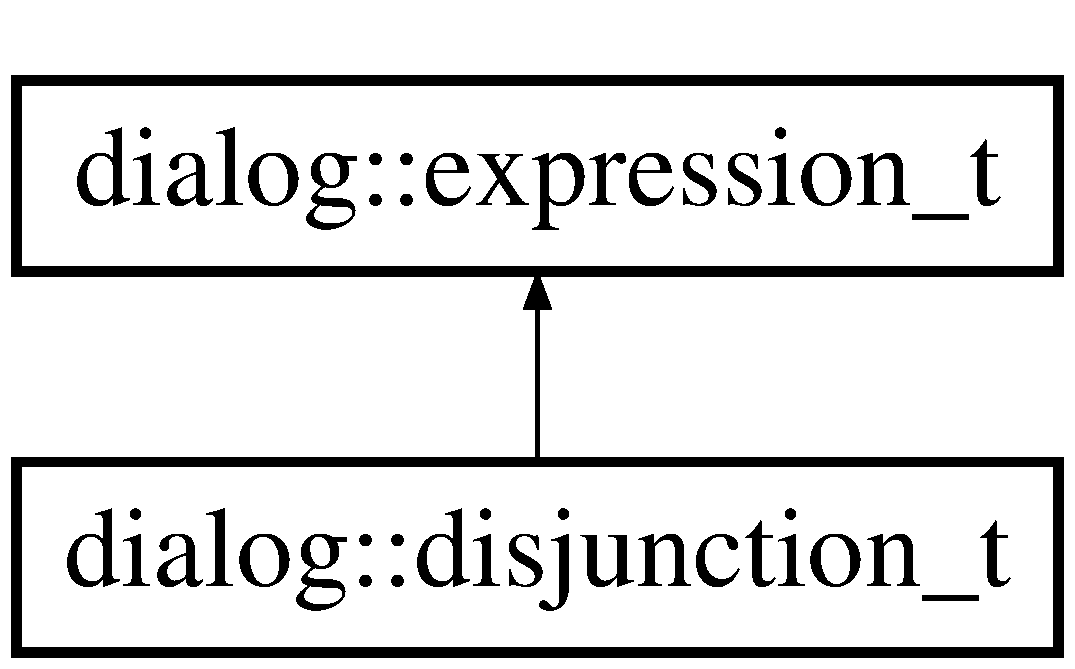
\includegraphics[height=2.000000cm]{structdialog_1_1disjunction__t}
\end{center}
\end{figure}
\subsection*{Public Member Functions}
\begin{DoxyCompactItemize}
\item 
\mbox{\Hypertarget{structdialog_1_1disjunction__t_aec8aa792702fd0da7d18cd473dc10ab7}\label{structdialog_1_1disjunction__t_aec8aa792702fd0da7d18cd473dc10ab7}} 
{\bfseries disjunction\+\_\+t} (\hyperlink{structdialog_1_1expression__t}{expression\+\_\+t} $\ast$l, \hyperlink{structdialog_1_1expression__t}{expression\+\_\+t} $\ast$r)
\end{DoxyCompactItemize}
\subsection*{Public Attributes}
\begin{DoxyCompactItemize}
\item 
\mbox{\Hypertarget{structdialog_1_1disjunction__t_af604bfee648d8c1914368fc18167c708}\label{structdialog_1_1disjunction__t_af604bfee648d8c1914368fc18167c708}} 
\hyperlink{structdialog_1_1expression__t}{expression\+\_\+t} $\ast$ {\bfseries left}
\item 
\mbox{\Hypertarget{structdialog_1_1disjunction__t_aa8f1bb1031ae3934b37237ff5f50eae6}\label{structdialog_1_1disjunction__t_aa8f1bb1031ae3934b37237ff5f50eae6}} 
\hyperlink{structdialog_1_1expression__t}{expression\+\_\+t} $\ast$ {\bfseries right}
\end{DoxyCompactItemize}


\subsection{Detailed Description}
Disjunction expression. 

The documentation for this struct was generated from the following file\+:\begin{DoxyCompactItemize}
\item 
/\+Users/neil/\+Documents/\+Berkeley/research/dialog/libdialog/dialog/expression.\+h\end{DoxyCompactItemize}

\hypertarget{structdialog_1_1storage_1_1durable}{}\section{dialog\+:\+:storage\+:\+:durable Struct Reference}
\label{structdialog_1_1storage_1_1durable}\index{dialog\+::storage\+::durable@{dialog\+::storage\+::durable}}


{\ttfamily \#include $<$storage.\+h$>$}

\subsection*{Static Public Member Functions}
\begin{DoxyCompactItemize}
\item 
static void $\ast$ \hyperlink{structdialog_1_1storage_1_1durable_ae22bc38ef79ba261079d36af562200fb}{allocate} (const std\+::string \&path, size\+\_\+t size)
\item 
static void \hyperlink{structdialog_1_1storage_1_1durable_a4fe38b9ca53b3cb89d53e5343f813db9}{free} (void $\ast$ptr, size\+\_\+t size)
\item 
static void \hyperlink{structdialog_1_1storage_1_1durable_a1ea22279109b5b06d195aadfe5594ef4}{flush} (void $\ast$ptr, size\+\_\+t size)
\end{DoxyCompactItemize}


\subsection{Detailed Description}
Durable (relaxed) storage mode, which allocates memory backed by a file, and also supports manually flushing of the data to the file. 

\subsection{Member Function Documentation}
\mbox{\Hypertarget{structdialog_1_1storage_1_1durable_ae22bc38ef79ba261079d36af562200fb}\label{structdialog_1_1storage_1_1durable_ae22bc38ef79ba261079d36af562200fb}} 
\index{dialog\+::storage\+::durable@{dialog\+::storage\+::durable}!allocate@{allocate}}
\index{allocate@{allocate}!dialog\+::storage\+::durable@{dialog\+::storage\+::durable}}
\subsubsection{\texorpdfstring{allocate()}{allocate()}}
{\footnotesize\ttfamily static void$\ast$ dialog\+::storage\+::durable\+::allocate (\begin{DoxyParamCaption}\item[{const std\+::string \&}]{path,  }\item[{size\+\_\+t}]{size }\end{DoxyParamCaption})\hspace{0.3cm}{\ttfamily [inline]}, {\ttfamily [static]}}

Allocates new memory backed by file. Creates the file, overwriting old data if the file already existed.


\begin{DoxyParams}{Parameters}
{\em path} & Backing file. \\
\hline
{\em size} & Size of requested memory. \\
\hline
\end{DoxyParams}
\mbox{\Hypertarget{structdialog_1_1storage_1_1durable_a1ea22279109b5b06d195aadfe5594ef4}\label{structdialog_1_1storage_1_1durable_a1ea22279109b5b06d195aadfe5594ef4}} 
\index{dialog\+::storage\+::durable@{dialog\+::storage\+::durable}!flush@{flush}}
\index{flush@{flush}!dialog\+::storage\+::durable@{dialog\+::storage\+::durable}}
\subsubsection{\texorpdfstring{flush()}{flush()}}
{\footnotesize\ttfamily static void dialog\+::storage\+::durable\+::flush (\begin{DoxyParamCaption}\item[{void $\ast$}]{ptr,  }\item[{size\+\_\+t}]{size }\end{DoxyParamCaption})\hspace{0.3cm}{\ttfamily [inline]}, {\ttfamily [static]}}

Flushes data to backed file (does nothing for this storage mode).


\begin{DoxyParams}{Parameters}
{\em ptr} & Pointer to memory. \\
\hline
{\em size} & Size of allocated memory. \\
\hline
\end{DoxyParams}
\mbox{\Hypertarget{structdialog_1_1storage_1_1durable_a4fe38b9ca53b3cb89d53e5343f813db9}\label{structdialog_1_1storage_1_1durable_a4fe38b9ca53b3cb89d53e5343f813db9}} 
\index{dialog\+::storage\+::durable@{dialog\+::storage\+::durable}!free@{free}}
\index{free@{free}!dialog\+::storage\+::durable@{dialog\+::storage\+::durable}}
\subsubsection{\texorpdfstring{free()}{free()}}
{\footnotesize\ttfamily static void dialog\+::storage\+::durable\+::free (\begin{DoxyParamCaption}\item[{void $\ast$}]{ptr,  }\item[{size\+\_\+t}]{size }\end{DoxyParamCaption})\hspace{0.3cm}{\ttfamily [inline]}, {\ttfamily [static]}}

Frees allocated memory. Does not delete backing file.


\begin{DoxyParams}{Parameters}
{\em ptr} & Pointer to memory to be freed. \\
\hline
{\em size} & Size of allocated memory. \\
\hline
\end{DoxyParams}


The documentation for this struct was generated from the following file\+:\begin{DoxyCompactItemize}
\item 
/\+Users/neil/\+Documents/\+Berkeley/research/dialog/libdialog/dialog/storage.\+h\end{DoxyCompactItemize}

\hypertarget{structdialog_1_1storage_1_1durable__relaxed}{}\section{dialog\+:\+:storage\+:\+:durable\+\_\+relaxed Struct Reference}
\label{structdialog_1_1storage_1_1durable__relaxed}\index{dialog\+::storage\+::durable\+\_\+relaxed@{dialog\+::storage\+::durable\+\_\+relaxed}}


{\ttfamily \#include $<$storage.\+h$>$}

\subsection*{Static Public Member Functions}
\begin{DoxyCompactItemize}
\item 
static void $\ast$ \hyperlink{structdialog_1_1storage_1_1durable__relaxed_a1067618bb9a7eae15a84642affcfcdd1}{allocate} (const std\+::string \&path, size\+\_\+t size)
\item 
static void \hyperlink{structdialog_1_1storage_1_1durable__relaxed_a7eee32ffcf5bd7a8da913f3cc5747579}{free} (void $\ast$ptr, size\+\_\+t size)
\item 
static void \hyperlink{structdialog_1_1storage_1_1durable__relaxed_a017593d30af37c9bb6df31c82dfbfcf5}{flush} (void $\ast$ptr, size\+\_\+t size)
\end{DoxyCompactItemize}


\subsection{Detailed Description}
Durable (relaxed) storage mode, which allocates memory backed by a file, but delegates flushing of the data to the file to the OS kernel. 

\subsection{Member Function Documentation}
\mbox{\Hypertarget{structdialog_1_1storage_1_1durable__relaxed_a1067618bb9a7eae15a84642affcfcdd1}\label{structdialog_1_1storage_1_1durable__relaxed_a1067618bb9a7eae15a84642affcfcdd1}} 
\index{dialog\+::storage\+::durable\+\_\+relaxed@{dialog\+::storage\+::durable\+\_\+relaxed}!allocate@{allocate}}
\index{allocate@{allocate}!dialog\+::storage\+::durable\+\_\+relaxed@{dialog\+::storage\+::durable\+\_\+relaxed}}
\subsubsection{\texorpdfstring{allocate()}{allocate()}}
{\footnotesize\ttfamily static void$\ast$ dialog\+::storage\+::durable\+\_\+relaxed\+::allocate (\begin{DoxyParamCaption}\item[{const std\+::string \&}]{path,  }\item[{size\+\_\+t}]{size }\end{DoxyParamCaption})\hspace{0.3cm}{\ttfamily [inline]}, {\ttfamily [static]}}

Allocates new memory backed by file. Creates the file, overwriting old data if the file already existed.


\begin{DoxyParams}{Parameters}
{\em path} & Backing file. \\
\hline
{\em size} & Size of requested memory. \\
\hline
\end{DoxyParams}
\mbox{\Hypertarget{structdialog_1_1storage_1_1durable__relaxed_a017593d30af37c9bb6df31c82dfbfcf5}\label{structdialog_1_1storage_1_1durable__relaxed_a017593d30af37c9bb6df31c82dfbfcf5}} 
\index{dialog\+::storage\+::durable\+\_\+relaxed@{dialog\+::storage\+::durable\+\_\+relaxed}!flush@{flush}}
\index{flush@{flush}!dialog\+::storage\+::durable\+\_\+relaxed@{dialog\+::storage\+::durable\+\_\+relaxed}}
\subsubsection{\texorpdfstring{flush()}{flush()}}
{\footnotesize\ttfamily static void dialog\+::storage\+::durable\+\_\+relaxed\+::flush (\begin{DoxyParamCaption}\item[{void $\ast$}]{ptr,  }\item[{size\+\_\+t}]{size }\end{DoxyParamCaption})\hspace{0.3cm}{\ttfamily [inline]}, {\ttfamily [static]}}

Flushes data to backed file (does nothing for this storage mode).


\begin{DoxyParams}{Parameters}
{\em ptr} & Pointer to memory. \\
\hline
{\em size} & Size of allocated memory. \\
\hline
\end{DoxyParams}
\mbox{\Hypertarget{structdialog_1_1storage_1_1durable__relaxed_a7eee32ffcf5bd7a8da913f3cc5747579}\label{structdialog_1_1storage_1_1durable__relaxed_a7eee32ffcf5bd7a8da913f3cc5747579}} 
\index{dialog\+::storage\+::durable\+\_\+relaxed@{dialog\+::storage\+::durable\+\_\+relaxed}!free@{free}}
\index{free@{free}!dialog\+::storage\+::durable\+\_\+relaxed@{dialog\+::storage\+::durable\+\_\+relaxed}}
\subsubsection{\texorpdfstring{free()}{free()}}
{\footnotesize\ttfamily static void dialog\+::storage\+::durable\+\_\+relaxed\+::free (\begin{DoxyParamCaption}\item[{void $\ast$}]{ptr,  }\item[{size\+\_\+t}]{size }\end{DoxyParamCaption})\hspace{0.3cm}{\ttfamily [inline]}, {\ttfamily [static]}}

Frees allocated memory. Does not delete backing file.


\begin{DoxyParams}{Parameters}
{\em ptr} & Pointer to memory to be freed. \\
\hline
{\em size} & Size of allocated memory. \\
\hline
\end{DoxyParams}


The documentation for this struct was generated from the following file\+:\begin{DoxyCompactItemize}
\item 
/\+Users/neil/\+Documents/\+Berkeley/research/dialog/libdialog/dialog/storage.\+h\end{DoxyCompactItemize}

\hypertarget{classdialog_1_1elias__gamma__encoded__array}{}\section{dialog\+:\+:elias\+\_\+gamma\+\_\+encoded\+\_\+array$<$ T, sampling\+\_\+rate $>$ Class Template Reference}
\label{classdialog_1_1elias__gamma__encoded__array}\index{dialog\+::elias\+\_\+gamma\+\_\+encoded\+\_\+array$<$ T, sampling\+\_\+rate $>$@{dialog\+::elias\+\_\+gamma\+\_\+encoded\+\_\+array$<$ T, sampling\+\_\+rate $>$}}
Inheritance diagram for dialog\+:\+:elias\+\_\+gamma\+\_\+encoded\+\_\+array$<$ T, sampling\+\_\+rate $>$\+:\begin{figure}[H]
\begin{center}
\leavevmode
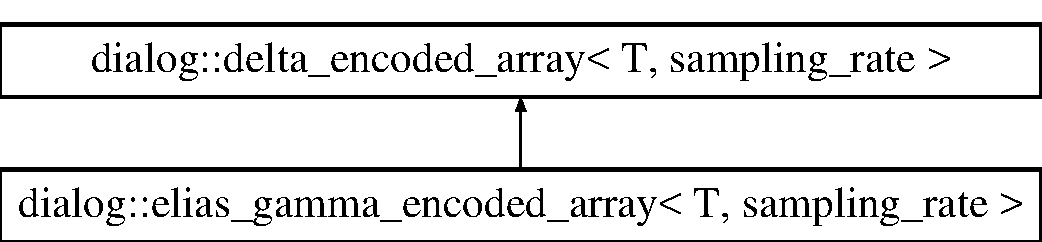
\includegraphics[height=2.000000cm]{classdialog_1_1elias__gamma__encoded__array}
\end{center}
\end{figure}
\subsection*{Public Types}
\begin{DoxyCompactItemize}
\item 
\mbox{\Hypertarget{classdialog_1_1elias__gamma__encoded__array_af927003f739a0ac6da1237a6ee1d45d4}\label{classdialog_1_1elias__gamma__encoded__array_af927003f739a0ac6da1237a6ee1d45d4}} 
typedef \hyperlink{classdialog_1_1delta__encoded__array}{delta\+\_\+encoded\+\_\+array}$<$ T $>$\+::size\+\_\+type {\bfseries size\+\_\+type}
\item 
\mbox{\Hypertarget{classdialog_1_1elias__gamma__encoded__array_a50628026535248b75fb77dc60bf0161b}\label{classdialog_1_1elias__gamma__encoded__array_a50628026535248b75fb77dc60bf0161b}} 
typedef \hyperlink{classdialog_1_1delta__encoded__array}{delta\+\_\+encoded\+\_\+array}$<$ T $>$\+::pos\+\_\+type {\bfseries pos\+\_\+type}
\item 
\mbox{\Hypertarget{classdialog_1_1elias__gamma__encoded__array_a430641490aac6e97f8df735b66cc6856}\label{classdialog_1_1elias__gamma__encoded__array_a430641490aac6e97f8df735b66cc6856}} 
typedef \hyperlink{classdialog_1_1delta__encoded__array}{delta\+\_\+encoded\+\_\+array}$<$ T $>$\+::width\+\_\+type {\bfseries width\+\_\+type}
\end{DoxyCompactItemize}
\subsection*{Public Member Functions}
\begin{DoxyCompactItemize}
\item 
\hyperlink{classdialog_1_1elias__gamma__encoded__array_a18b53f9744c7c0c0a1d0e5a77ffcb840}{elias\+\_\+gamma\+\_\+encoded\+\_\+array} ()
\item 
\hyperlink{classdialog_1_1elias__gamma__encoded__array_a65bed69251739947eabd7e0a157b8923}{elias\+\_\+gamma\+\_\+encoded\+\_\+array} (T $\ast$elements, size\+\_\+type num\+\_\+elements)
\item 
T \hyperlink{classdialog_1_1elias__gamma__encoded__array_a34a2e347fc7b8c7091590a457954522c}{get} (pos\+\_\+type i)
\item 
T \hyperlink{classdialog_1_1elias__gamma__encoded__array_ab9a186f942d1ce70c7a03b5b5a97fdbc}{operator\mbox{[}$\,$\mbox{]}} (pos\+\_\+type i)
\end{DoxyCompactItemize}
\subsection*{Additional Inherited Members}


\subsection{Constructor \& Destructor Documentation}
\mbox{\Hypertarget{classdialog_1_1elias__gamma__encoded__array_a18b53f9744c7c0c0a1d0e5a77ffcb840}\label{classdialog_1_1elias__gamma__encoded__array_a18b53f9744c7c0c0a1d0e5a77ffcb840}} 
\index{dialog\+::elias\+\_\+gamma\+\_\+encoded\+\_\+array@{dialog\+::elias\+\_\+gamma\+\_\+encoded\+\_\+array}!elias\+\_\+gamma\+\_\+encoded\+\_\+array@{elias\+\_\+gamma\+\_\+encoded\+\_\+array}}
\index{elias\+\_\+gamma\+\_\+encoded\+\_\+array@{elias\+\_\+gamma\+\_\+encoded\+\_\+array}!dialog\+::elias\+\_\+gamma\+\_\+encoded\+\_\+array@{dialog\+::elias\+\_\+gamma\+\_\+encoded\+\_\+array}}
\subsubsection{\texorpdfstring{elias\+\_\+gamma\+\_\+encoded\+\_\+array()}{elias\_gamma\_encoded\_array()}\hspace{0.1cm}{\footnotesize\ttfamily [1/2]}}
{\footnotesize\ttfamily template$<$typename T , uint32\+\_\+t sampling\+\_\+rate = 128$>$ \\
\hyperlink{classdialog_1_1elias__gamma__encoded__array}{dialog\+::elias\+\_\+gamma\+\_\+encoded\+\_\+array}$<$ T, sampling\+\_\+rate $>$\+::\hyperlink{classdialog_1_1elias__gamma__encoded__array}{elias\+\_\+gamma\+\_\+encoded\+\_\+array} (\begin{DoxyParamCaption}{ }\end{DoxyParamCaption})\hspace{0.3cm}{\ttfamily [inline]}}

Default constructor that initializes the encoded array \mbox{\Hypertarget{classdialog_1_1elias__gamma__encoded__array_a65bed69251739947eabd7e0a157b8923}\label{classdialog_1_1elias__gamma__encoded__array_a65bed69251739947eabd7e0a157b8923}} 
\index{dialog\+::elias\+\_\+gamma\+\_\+encoded\+\_\+array@{dialog\+::elias\+\_\+gamma\+\_\+encoded\+\_\+array}!elias\+\_\+gamma\+\_\+encoded\+\_\+array@{elias\+\_\+gamma\+\_\+encoded\+\_\+array}}
\index{elias\+\_\+gamma\+\_\+encoded\+\_\+array@{elias\+\_\+gamma\+\_\+encoded\+\_\+array}!dialog\+::elias\+\_\+gamma\+\_\+encoded\+\_\+array@{dialog\+::elias\+\_\+gamma\+\_\+encoded\+\_\+array}}
\subsubsection{\texorpdfstring{elias\+\_\+gamma\+\_\+encoded\+\_\+array()}{elias\_gamma\_encoded\_array()}\hspace{0.1cm}{\footnotesize\ttfamily [2/2]}}
{\footnotesize\ttfamily template$<$typename T , uint32\+\_\+t sampling\+\_\+rate = 128$>$ \\
\hyperlink{classdialog_1_1elias__gamma__encoded__array}{dialog\+::elias\+\_\+gamma\+\_\+encoded\+\_\+array}$<$ T, sampling\+\_\+rate $>$\+::\hyperlink{classdialog_1_1elias__gamma__encoded__array}{elias\+\_\+gamma\+\_\+encoded\+\_\+array} (\begin{DoxyParamCaption}\item[{T $\ast$}]{elements,  }\item[{size\+\_\+type}]{num\+\_\+elements }\end{DoxyParamCaption})\hspace{0.3cm}{\ttfamily [inline]}}

Constructor that initializes data and size of the array 
\begin{DoxyParams}{Parameters}
{\em elements} & The elements of the data \\
\hline
{\em num\+\_\+elements} & The number of elements in the array \\
\hline
\end{DoxyParams}


\subsection{Member Function Documentation}
\mbox{\Hypertarget{classdialog_1_1elias__gamma__encoded__array_a34a2e347fc7b8c7091590a457954522c}\label{classdialog_1_1elias__gamma__encoded__array_a34a2e347fc7b8c7091590a457954522c}} 
\index{dialog\+::elias\+\_\+gamma\+\_\+encoded\+\_\+array@{dialog\+::elias\+\_\+gamma\+\_\+encoded\+\_\+array}!get@{get}}
\index{get@{get}!dialog\+::elias\+\_\+gamma\+\_\+encoded\+\_\+array@{dialog\+::elias\+\_\+gamma\+\_\+encoded\+\_\+array}}
\subsubsection{\texorpdfstring{get()}{get()}}
{\footnotesize\ttfamily template$<$typename T , uint32\+\_\+t sampling\+\_\+rate = 128$>$ \\
T \hyperlink{classdialog_1_1elias__gamma__encoded__array}{dialog\+::elias\+\_\+gamma\+\_\+encoded\+\_\+array}$<$ T, sampling\+\_\+rate $>$\+::get (\begin{DoxyParamCaption}\item[{pos\+\_\+type}]{i }\end{DoxyParamCaption})\hspace{0.3cm}{\ttfamily [inline]}}

Gets the element at the specified index 
\begin{DoxyParams}{Parameters}
{\em i} & The index \\
\hline
\end{DoxyParams}
\begin{DoxyReturn}{Returns}
The value at that index 
\end{DoxyReturn}
\mbox{\Hypertarget{classdialog_1_1elias__gamma__encoded__array_ab9a186f942d1ce70c7a03b5b5a97fdbc}\label{classdialog_1_1elias__gamma__encoded__array_ab9a186f942d1ce70c7a03b5b5a97fdbc}} 
\index{dialog\+::elias\+\_\+gamma\+\_\+encoded\+\_\+array@{dialog\+::elias\+\_\+gamma\+\_\+encoded\+\_\+array}!operator\mbox{[}\mbox{]}@{operator[]}}
\index{operator\mbox{[}\mbox{]}@{operator[]}!dialog\+::elias\+\_\+gamma\+\_\+encoded\+\_\+array@{dialog\+::elias\+\_\+gamma\+\_\+encoded\+\_\+array}}
\subsubsection{\texorpdfstring{operator[]()}{operator[]()}}
{\footnotesize\ttfamily template$<$typename T , uint32\+\_\+t sampling\+\_\+rate = 128$>$ \\
T \hyperlink{classdialog_1_1elias__gamma__encoded__array}{dialog\+::elias\+\_\+gamma\+\_\+encoded\+\_\+array}$<$ T, sampling\+\_\+rate $>$\+::operator\mbox{[}$\,$\mbox{]} (\begin{DoxyParamCaption}\item[{pos\+\_\+type}]{i }\end{DoxyParamCaption})\hspace{0.3cm}{\ttfamily [inline]}}

Accesses the array at the specified index 
\begin{DoxyParams}{Parameters}
{\em i} & The index \\
\hline
\end{DoxyParams}
\begin{DoxyReturn}{Returns}
The value at that index 
\end{DoxyReturn}


The documentation for this class was generated from the following file\+:\begin{DoxyCompactItemize}
\item 
/\+Users/neil/\+Documents/\+Berkeley/research/dialog/libdialog/dialog/delta\+\_\+encoded\+\_\+array.\+h\end{DoxyCompactItemize}

\hypertarget{structdialog_1_1index_1_1empty__stats}{}\section{dialog\+:\+:index\+:\+:empty\+\_\+stats Struct Reference}
\label{structdialog_1_1index_1_1empty__stats}\index{dialog\+::index\+::empty\+\_\+stats@{dialog\+::index\+::empty\+\_\+stats}}
\subsection*{Public Member Functions}
\begin{DoxyCompactItemize}
\item 
\mbox{\Hypertarget{structdialog_1_1index_1_1empty__stats_a7c00752571aa457e561a9e97202a4b32}\label{structdialog_1_1index_1_1empty__stats_a7c00752571aa457e561a9e97202a4b32}} 
{\bfseries empty\+\_\+stats} (const \hyperlink{structdialog_1_1index_1_1empty__stats}{empty\+\_\+stats} \&other)
\end{DoxyCompactItemize}


The documentation for this struct was generated from the following file\+:\begin{DoxyCompactItemize}
\item 
/\+Users/neil/\+Documents/\+Berkeley/research/dialog/libdialog/dialog/tiered\+\_\+index.\+h\end{DoxyCompactItemize}

\hypertarget{classdialog_1_1expression__compiler}{}\section{dialog\+:\+:expression\+\_\+compiler Class Reference}
\label{classdialog_1_1expression__compiler}\index{dialog\+::expression\+\_\+compiler@{dialog\+::expression\+\_\+compiler}}
\subsection*{Static Public Member Functions}
\begin{DoxyCompactItemize}
\item 
\mbox{\Hypertarget{classdialog_1_1expression__compiler_aa142fb4f61014a6e7403ee901bde646b}\label{classdialog_1_1expression__compiler_aa142fb4f61014a6e7403ee901bde646b}} 
{\footnotesize template$<$typename schema\+\_\+t $>$ }\\static \hyperlink{structdialog_1_1compiled__expression}{compiled\+\_\+expression} {\bfseries compile} (\hyperlink{structdialog_1_1expression__t}{expression\+\_\+t} $\ast$exp, const \hyperlink{classdialog_1_1schema__t}{schema\+\_\+t} \&schema)
\item 
\mbox{\Hypertarget{classdialog_1_1expression__compiler_a333615d4926a13c06ae9a254a43b12cd}\label{classdialog_1_1expression__compiler_a333615d4926a13c06ae9a254a43b12cd}} 
{\footnotesize template$<$typename schema\+\_\+t $>$ }\\static void {\bfseries compile} (\hyperlink{structdialog_1_1compiled__expression}{compiled\+\_\+expression} \&cexp, \hyperlink{structdialog_1_1expression__t}{expression\+\_\+t} $\ast$exp, const \hyperlink{classdialog_1_1schema__t}{schema\+\_\+t} \&schema)
\item 
\mbox{\Hypertarget{classdialog_1_1expression__compiler_a17ff2d529e43cec1be451f52a1f4ab60}\label{classdialog_1_1expression__compiler_a17ff2d529e43cec1be451f52a1f4ab60}} 
{\footnotesize template$<$typename schema\+\_\+t $>$ }\\static \hyperlink{structdialog_1_1compiled__expression}{compiled\+\_\+expression} {\bfseries compile} (const std\+::string \&exp, const \hyperlink{classdialog_1_1schema__t}{schema\+\_\+t} \&schema)
\item 
\mbox{\Hypertarget{classdialog_1_1expression__compiler_ac0169a4a67653a455c4e0309aafedb1e}\label{classdialog_1_1expression__compiler_ac0169a4a67653a455c4e0309aafedb1e}} 
{\footnotesize template$<$typename schema\+\_\+t $>$ }\\static void {\bfseries compile} (\hyperlink{structdialog_1_1compiled__expression}{compiled\+\_\+expression} \&minterms, const std\+::string \&exp, const \hyperlink{classdialog_1_1schema__t}{schema\+\_\+t} \&schema)
\end{DoxyCompactItemize}


The documentation for this class was generated from the following file\+:\begin{DoxyCompactItemize}
\item 
/\+Users/neil/\+Documents/\+Berkeley/research/dialog/libdialog/dialog/expression\+\_\+compiler.\+h\end{DoxyCompactItemize}

\hypertarget{structdialog_1_1expression__lex__token}{}\section{dialog\+:\+:expression\+\_\+lex\+\_\+token Struct Reference}
\label{structdialog_1_1expression__lex__token}\index{dialog\+::expression\+\_\+lex\+\_\+token@{dialog\+::expression\+\_\+lex\+\_\+token}}


{\ttfamily \#include $<$expression.\+h$>$}

\subsection*{Public Member Functions}
\begin{DoxyCompactItemize}
\item 
\mbox{\Hypertarget{structdialog_1_1expression__lex__token_aac6ebd20c98fd48fd86f232448976570}\label{structdialog_1_1expression__lex__token_aac6ebd20c98fd48fd86f232448976570}} 
{\bfseries expression\+\_\+lex\+\_\+token} (const int i, const std\+::string \&val)
\end{DoxyCompactItemize}
\subsection*{Public Attributes}
\begin{DoxyCompactItemize}
\item 
\mbox{\Hypertarget{structdialog_1_1expression__lex__token_a2bfc13d1160ec976f2476d828636581a}\label{structdialog_1_1expression__lex__token_a2bfc13d1160ec976f2476d828636581a}} 
const int {\bfseries id}
\item 
\mbox{\Hypertarget{structdialog_1_1expression__lex__token_aefc12495fa2e870b10a8fc38c6bf5ef7}\label{structdialog_1_1expression__lex__token_aefc12495fa2e870b10a8fc38c6bf5ef7}} 
const std\+::string {\bfseries value}
\end{DoxyCompactItemize}


\subsection{Detailed Description}
Token generated by lexer. 

The documentation for this struct was generated from the following file\+:\begin{DoxyCompactItemize}
\item 
/\+Users/neil/\+Documents/\+Berkeley/research/dialog/libdialog/dialog/expression.\+h\end{DoxyCompactItemize}

\hypertarget{classdialog_1_1expression__lexer}{}\section{dialog\+:\+:expression\+\_\+lexer Class Reference}
\label{classdialog_1_1expression__lexer}\index{dialog\+::expression\+\_\+lexer@{dialog\+::expression\+\_\+lexer}}


{\ttfamily \#include $<$expression.\+h$>$}

\subsection*{Public Member Functions}
\begin{DoxyCompactItemize}
\item 
\mbox{\Hypertarget{classdialog_1_1expression__lexer_a19dbd63a6fb6c87b66bde397bca5c875}\label{classdialog_1_1expression__lexer_a19dbd63a6fb6c87b66bde397bca5c875}} 
{\bfseries expression\+\_\+lexer} (const std\+::string \&exp)
\item 
\mbox{\Hypertarget{classdialog_1_1expression__lexer_a0b5966eb1b0f0d3d5f3e40c0fdd3d868}\label{classdialog_1_1expression__lexer_a0b5966eb1b0f0d3d5f3e40c0fdd3d868}} 
void {\bfseries str} (const std\+::string \&exp)
\item 
\mbox{\Hypertarget{classdialog_1_1expression__lexer_a64a4ab732ed88c5139f59f261a7e4aac}\label{classdialog_1_1expression__lexer_a64a4ab732ed88c5139f59f261a7e4aac}} 
size\+\_\+t {\bfseries pos} ()
\item 
\mbox{\Hypertarget{classdialog_1_1expression__lexer_aa3a15848d2562dc6901adfdc0aaf42ae}\label{classdialog_1_1expression__lexer_aa3a15848d2562dc6901adfdc0aaf42ae}} 
std\+::string {\bfseries str} ()
\item 
\mbox{\Hypertarget{classdialog_1_1expression__lexer_ac76253b8c049a7e6899acc765be9c9b4}\label{classdialog_1_1expression__lexer_ac76253b8c049a7e6899acc765be9c9b4}} 
const \hyperlink{structdialog_1_1expression__lex__token}{expression\+\_\+lex\+\_\+token} {\bfseries next\+\_\+token} ()
\item 
\mbox{\Hypertarget{classdialog_1_1expression__lexer_a4810e4e4090270c369784a431bde614a}\label{classdialog_1_1expression__lexer_a4810e4e4090270c369784a431bde614a}} 
const \hyperlink{structdialog_1_1expression__lex__token}{expression\+\_\+lex\+\_\+token} {\bfseries peek\+\_\+token} ()
\item 
\mbox{\Hypertarget{classdialog_1_1expression__lexer_a40cf6a7ea967e8abeb2dbc23f4e76aed}\label{classdialog_1_1expression__lexer_a40cf6a7ea967e8abeb2dbc23f4e76aed}} 
void {\bfseries put\+\_\+back} (const \hyperlink{structdialog_1_1expression__lex__token}{expression\+\_\+lex\+\_\+token} \&tok)
\end{DoxyCompactItemize}
\subsection*{Static Public Attributes}
\begin{DoxyCompactItemize}
\item 
\mbox{\Hypertarget{classdialog_1_1expression__lexer_a8a3c153f50a0b5ecd4158bffb9467a9c}\label{classdialog_1_1expression__lexer_a8a3c153f50a0b5ecd4158bffb9467a9c}} 
static const int {\bfseries I\+N\+V\+A\+L\+ID} = -\/2
\item 
\mbox{\Hypertarget{classdialog_1_1expression__lexer_a080a9a2bb30395f27786cc6c652802d0}\label{classdialog_1_1expression__lexer_a080a9a2bb30395f27786cc6c652802d0}} 
static const int {\bfseries E\+ND} = -\/1
\item 
\mbox{\Hypertarget{classdialog_1_1expression__lexer_a0c271fa07c268b177cf9422a9dc62ddf}\label{classdialog_1_1expression__lexer_a0c271fa07c268b177cf9422a9dc62ddf}} 
static const int {\bfseries OR} = 0
\item 
\mbox{\Hypertarget{classdialog_1_1expression__lexer_a5c5af973665a5ad0f84594bc60e19985}\label{classdialog_1_1expression__lexer_a5c5af973665a5ad0f84594bc60e19985}} 
static const int {\bfseries A\+ND} = 1
\item 
\mbox{\Hypertarget{classdialog_1_1expression__lexer_a0e5fda1ce8991fee059dccc924c03d90}\label{classdialog_1_1expression__lexer_a0e5fda1ce8991fee059dccc924c03d90}} 
static const int {\bfseries N\+OT} = 2
\item 
\mbox{\Hypertarget{classdialog_1_1expression__lexer_af7dd279996995b7c0e5ee4315f75ec61}\label{classdialog_1_1expression__lexer_af7dd279996995b7c0e5ee4315f75ec61}} 
static const int {\bfseries L\+E\+FT} = 3
\item 
\mbox{\Hypertarget{classdialog_1_1expression__lexer_a9bc7735c32393c063f53ef172407827a}\label{classdialog_1_1expression__lexer_a9bc7735c32393c063f53ef172407827a}} 
static const int {\bfseries R\+I\+G\+HT} = 4
\item 
\mbox{\Hypertarget{classdialog_1_1expression__lexer_a51173760a05683729ff9ee71c9278f5e}\label{classdialog_1_1expression__lexer_a51173760a05683729ff9ee71c9278f5e}} 
static const int {\bfseries O\+P\+E\+R\+A\+T\+OR} = 5
\item 
\mbox{\Hypertarget{classdialog_1_1expression__lexer_a841fb8469c5370606435e9c4dbc4e453}\label{classdialog_1_1expression__lexer_a841fb8469c5370606435e9c4dbc4e453}} 
static const int {\bfseries O\+P\+E\+R\+A\+ND} = 6
\end{DoxyCompactItemize}


\subsection{Detailed Description}
Lexer for the expression. 

The documentation for this class was generated from the following file\+:\begin{DoxyCompactItemize}
\item 
/\+Users/neil/\+Documents/\+Berkeley/research/dialog/libdialog/dialog/expression.\+h\end{DoxyCompactItemize}

\hypertarget{classdialog_1_1expression__parser}{}\section{dialog\+:\+:expression\+\_\+parser Class Reference}
\label{classdialog_1_1expression__parser}\index{dialog\+::expression\+\_\+parser@{dialog\+::expression\+\_\+parser}}


{\ttfamily \#include $<$expression.\+h$>$}

\subsection*{Public Member Functions}
\begin{DoxyCompactItemize}
\item 
\mbox{\Hypertarget{classdialog_1_1expression__parser_a93775653658b4168d4089e9f1cde83a6}\label{classdialog_1_1expression__parser_a93775653658b4168d4089e9f1cde83a6}} 
{\bfseries expression\+\_\+parser} (const std\+::string \&exp)
\item 
\mbox{\Hypertarget{classdialog_1_1expression__parser_ac91fd93bee7e2e9b3a3e0fc232523bfc}\label{classdialog_1_1expression__parser_ac91fd93bee7e2e9b3a3e0fc232523bfc}} 
\hyperlink{structdialog_1_1expression__t}{expression\+\_\+t} $\ast$ {\bfseries parse} ()
\end{DoxyCompactItemize}


\subsection{Detailed Description}
Parser for the expression. 

The documentation for this class was generated from the following file\+:\begin{DoxyCompactItemize}
\item 
/\+Users/neil/\+Documents/\+Berkeley/research/dialog/libdialog/dialog/expression.\+h\end{DoxyCompactItemize}

\hypertarget{structdialog_1_1expression__t}{}\section{dialog\+:\+:expression\+\_\+t Struct Reference}
\label{structdialog_1_1expression__t}\index{dialog\+::expression\+\_\+t@{dialog\+::expression\+\_\+t}}


{\ttfamily \#include $<$expression.\+h$>$}

Inheritance diagram for dialog\+:\+:expression\+\_\+t\+:\begin{figure}[H]
\begin{center}
\leavevmode
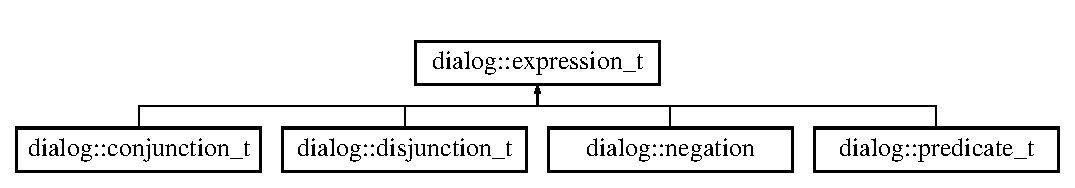
\includegraphics[height=2.000000cm]{structdialog_1_1expression__t}
\end{center}
\end{figure}
\subsection*{Public Member Functions}
\begin{DoxyCompactItemize}
\item 
\mbox{\Hypertarget{structdialog_1_1expression__t_a160723f49579e321986ab217777a8238}\label{structdialog_1_1expression__t_a160723f49579e321986ab217777a8238}} 
{\bfseries expression\+\_\+t} (expression\+\_\+id eid)
\end{DoxyCompactItemize}
\subsection*{Public Attributes}
\begin{DoxyCompactItemize}
\item 
\mbox{\Hypertarget{structdialog_1_1expression__t_a73271728ad2081b7bdaf00f7051eef66}\label{structdialog_1_1expression__t_a73271728ad2081b7bdaf00f7051eef66}} 
expression\+\_\+id {\bfseries id}
\end{DoxyCompactItemize}


\subsection{Detailed Description}
Generic expression. 

The documentation for this struct was generated from the following file\+:\begin{DoxyCompactItemize}
\item 
/\+Users/neil/\+Documents/\+Berkeley/research/dialog/libdialog/dialog/expression.\+h\end{DoxyCompactItemize}

\hypertarget{classdialog_1_1expression__utils}{}\section{dialog\+:\+:expression\+\_\+utils Class Reference}
\label{classdialog_1_1expression__utils}\index{dialog\+::expression\+\_\+utils@{dialog\+::expression\+\_\+utils}}


{\ttfamily \#include $<$expression.\+h$>$}

\subsection*{Static Public Member Functions}
\begin{DoxyCompactItemize}
\item 
static void \hyperlink{classdialog_1_1expression__utils_ab26b15dece4bf0ab5f0879d397b15ad1}{print\+\_\+expression} (\hyperlink{structdialog_1_1expression__t}{expression\+\_\+t} $\ast$exp)
\item 
static void \hyperlink{classdialog_1_1expression__utils_aa077b3345553c3c71674c2577eebf143}{free\+\_\+expression} (\hyperlink{structdialog_1_1expression__t}{expression\+\_\+t} $\ast$exp)
\end{DoxyCompactItemize}


\subsection{Detailed Description}
Expression utilities. 

\subsection{Member Function Documentation}
\mbox{\Hypertarget{classdialog_1_1expression__utils_aa077b3345553c3c71674c2577eebf143}\label{classdialog_1_1expression__utils_aa077b3345553c3c71674c2577eebf143}} 
\index{dialog\+::expression\+\_\+utils@{dialog\+::expression\+\_\+utils}!free\+\_\+expression@{free\+\_\+expression}}
\index{free\+\_\+expression@{free\+\_\+expression}!dialog\+::expression\+\_\+utils@{dialog\+::expression\+\_\+utils}}
\subsubsection{\texorpdfstring{free\+\_\+expression()}{free\_expression()}}
{\footnotesize\ttfamily static void dialog\+::expression\+\_\+utils\+::free\+\_\+expression (\begin{DoxyParamCaption}\item[{\hyperlink{structdialog_1_1expression__t}{expression\+\_\+t} $\ast$}]{exp }\end{DoxyParamCaption})\hspace{0.3cm}{\ttfamily [inline]}, {\ttfamily [static]}}

Frees a given expression tree.


\begin{DoxyParams}{Parameters}
{\em exp} & Expression tree to free. \\
\hline
\end{DoxyParams}
\mbox{\Hypertarget{classdialog_1_1expression__utils_ab26b15dece4bf0ab5f0879d397b15ad1}\label{classdialog_1_1expression__utils_ab26b15dece4bf0ab5f0879d397b15ad1}} 
\index{dialog\+::expression\+\_\+utils@{dialog\+::expression\+\_\+utils}!print\+\_\+expression@{print\+\_\+expression}}
\index{print\+\_\+expression@{print\+\_\+expression}!dialog\+::expression\+\_\+utils@{dialog\+::expression\+\_\+utils}}
\subsubsection{\texorpdfstring{print\+\_\+expression()}{print\_expression()}}
{\footnotesize\ttfamily static void dialog\+::expression\+\_\+utils\+::print\+\_\+expression (\begin{DoxyParamCaption}\item[{\hyperlink{structdialog_1_1expression__t}{expression\+\_\+t} $\ast$}]{exp }\end{DoxyParamCaption})\hspace{0.3cm}{\ttfamily [inline]}, {\ttfamily [static]}}

Prints out a given expression tree.


\begin{DoxyParams}{Parameters}
{\em exp} & The expression tree to print. \\
\hline
\end{DoxyParams}


The documentation for this class was generated from the following file\+:\begin{DoxyCompactItemize}
\item 
/\+Users/neil/\+Documents/\+Berkeley/research/dialog/libdialog/dialog/expression.\+h\end{DoxyCompactItemize}

\hypertarget{structdialog_1_1field__t}{}\section{dialog\+:\+:field\+\_\+t Struct Reference}
\label{structdialog_1_1field__t}\index{dialog\+::field\+\_\+t@{dialog\+::field\+\_\+t}}
\subsection*{Public Member Functions}
\begin{DoxyCompactItemize}
\item 
\mbox{\Hypertarget{structdialog_1_1field__t_a38a5eac5a33bbc109cea5bec52243cf5}\label{structdialog_1_1field__t_a38a5eac5a33bbc109cea5bec52243cf5}} 
{\bfseries field\+\_\+t} (uint16\+\_\+t idx, const \hyperlink{structdialog_1_1data__type}{data\+\_\+type} \&type, void $\ast$\hyperlink{structdialog_1_1data}{data}, bool indexed, uint16\+\_\+t index\+\_\+id, double index\+\_\+bucket\+\_\+size)
\item 
\mbox{\Hypertarget{structdialog_1_1field__t_a37cb00c5b29296d901388b87077ae0a4}\label{structdialog_1_1field__t_a37cb00c5b29296d901388b87077ae0a4}} 
uint16\+\_\+t {\bfseries idx} () const
\item 
\mbox{\Hypertarget{structdialog_1_1field__t_a901ef5f8265f4e193e9e2395230b1722}\label{structdialog_1_1field__t_a901ef5f8265f4e193e9e2395230b1722}} 
const \hyperlink{structdialog_1_1data__type}{data\+\_\+type} \& {\bfseries type} () const
\item 
\mbox{\Hypertarget{structdialog_1_1field__t_a48b79aa56c9eec18e9be879a44531edb}\label{structdialog_1_1field__t_a48b79aa56c9eec18e9be879a44531edb}} 
const \hyperlink{classdialog_1_1immutable__value}{immutable\+\_\+value} \& {\bfseries value} () const
\item 
\mbox{\Hypertarget{structdialog_1_1field__t_a5c16ba60671457adc119b3877bb14887}\label{structdialog_1_1field__t_a5c16ba60671457adc119b3877bb14887}} 
bool {\bfseries is\+\_\+indexed} () const
\item 
\mbox{\Hypertarget{structdialog_1_1field__t_a200bca9e8bc82f756f202eb45555c199}\label{structdialog_1_1field__t_a200bca9e8bc82f756f202eb45555c199}} 
uint16\+\_\+t {\bfseries index\+\_\+id} () const
\item 
\mbox{\Hypertarget{structdialog_1_1field__t_a0ed25ca8c151d86486a2d19be42dcd14}\label{structdialog_1_1field__t_a0ed25ca8c151d86486a2d19be42dcd14}} 
\hyperlink{classdialog_1_1byte__string}{byte\+\_\+string} {\bfseries get\+\_\+key} () const
\item 
\mbox{\Hypertarget{structdialog_1_1field__t_adec7e0f179006c4ffa5398b6d220deb8}\label{structdialog_1_1field__t_adec7e0f179006c4ffa5398b6d220deb8}} 
{\footnotesize template$<$typename T $>$ }\\T {\bfseries as} () const
\item 
\mbox{\Hypertarget{structdialog_1_1field__t_af9be89078c159b53f29c4787ee85fd4d}\label{structdialog_1_1field__t_af9be89078c159b53f29c4787ee85fd4d}} 
std\+::string {\bfseries to\+\_\+string} () const
\end{DoxyCompactItemize}


The documentation for this struct was generated from the following file\+:\begin{DoxyCompactItemize}
\item 
/\+Users/neil/\+Documents/\+Berkeley/research/dialog/libdialog/dialog/field.\+h\end{DoxyCompactItemize}

\hypertarget{classdialog_1_1monitor_1_1filter}{}\section{dialog\+:\+:monitor\+:\+:filter Class Reference}
\label{classdialog_1_1monitor_1_1filter}\index{dialog\+::monitor\+::filter@{dialog\+::monitor\+::filter}}


{\ttfamily \#include $<$filter.\+h$>$}

\subsection*{Public Types}
\begin{DoxyCompactItemize}
\item 
\mbox{\Hypertarget{classdialog_1_1monitor_1_1filter_ab7625fee3176adc27d81874ef07e286c}\label{classdialog_1_1monitor_1_1filter_ab7625fee3176adc27d81874ef07e286c}} 
typedef \hyperlink{classdialog_1_1index_1_1radix__tree}{index\+::radix\+\_\+tree}$<$ \hyperlink{classdialog_1_1aggregated__reflog}{aggregated\+\_\+reflog} $>$ {\bfseries idx\+\_\+t}
\item 
\mbox{\Hypertarget{classdialog_1_1monitor_1_1filter_a41a5af5773b4c0576171823801f6829c}\label{classdialog_1_1monitor_1_1filter_a41a5af5773b4c0576171823801f6829c}} 
typedef \hyperlink{classflattened__container}{idx\+\_\+t\+::rt\+\_\+result} {\bfseries range\+\_\+result}
\end{DoxyCompactItemize}
\subsection*{Public Member Functions}
\begin{DoxyCompactItemize}
\item 
\hyperlink{classdialog_1_1monitor_1_1filter_a7fe577f3fc937bef2d62cbcf9c7b6662}{filter} (const \hyperlink{structdialog_1_1compiled__expression}{compiled\+\_\+expression} \&exp, filter\+\_\+fn fn=default\+\_\+filter)
\item 
\hyperlink{classdialog_1_1monitor_1_1filter_a5fa052157aa824765614c7de106a11c2}{filter} (filter\+\_\+fn fn=default\+\_\+filter)
\item 
size\+\_\+t \hyperlink{classdialog_1_1monitor_1_1filter_a6663e4c56880482de42a3366be94356d}{add\+\_\+trigger} (\hyperlink{structdialog_1_1monitor_1_1trigger}{trigger} $\ast$t)
\item 
bool \hyperlink{classdialog_1_1monitor_1_1filter_ac5c01fdc260a434815ab2bbd66ae9ab5}{remove\+\_\+trigger} (size\+\_\+t id)
\item 
\mbox{\Hypertarget{classdialog_1_1monitor_1_1filter_a8171f52c8ca67d8bc1f0b1fcb2eff525}\label{classdialog_1_1monitor_1_1filter_a8171f52c8ca67d8bc1f0b1fcb2eff525}} 
\hyperlink{structdialog_1_1monitor_1_1trigger}{trigger} $\ast$ {\bfseries get\+\_\+trigger} (size\+\_\+t id)
\item 
size\+\_\+t \hyperlink{classdialog_1_1monitor_1_1filter_aa84bc2df90155d5fd462dce52d86de5c}{num\+\_\+triggers} ()
\item 
void \hyperlink{classdialog_1_1monitor_1_1filter_a9daf4fdb82ff01d211a417e1531461e2}{update} (const \hyperlink{structdialog_1_1record__t}{record\+\_\+t} \&r)
\item 
void \hyperlink{classdialog_1_1monitor_1_1filter_ad0aba175b70f3bf63c4f0f83b5888ccf}{update} (size\+\_\+t log\+\_\+offset, const \hyperlink{classdialog_1_1schema__snapshot}{schema\+\_\+snapshot} \&snap, \hyperlink{structdialog_1_1record__block}{record\+\_\+block} \&block, size\+\_\+t record\+\_\+size)
\item 
\hyperlink{classdialog_1_1aggregated__reflog}{aggregated\+\_\+reflog} const  $\ast$ \hyperlink{classdialog_1_1monitor_1_1filter_a9e112bf3e11d7a02fdb5d49ed51a9827}{lookup} (uint64\+\_\+t ts\+\_\+block) const
\item 
\hyperlink{classflattened__container}{range\+\_\+result} \hyperlink{classdialog_1_1monitor_1_1filter_a5523a17cb88d0f5bd6b78bb16c085632}{lookup\+\_\+range} (uint64\+\_\+t ts\+\_\+block\+\_\+begin, uint64\+\_\+t ts\+\_\+block\+\_\+end) const
\item 
\mbox{\Hypertarget{classdialog_1_1monitor_1_1filter_a4bbf4488202299895570ce5d7ac9a76f}\label{classdialog_1_1monitor_1_1filter_a4bbf4488202299895570ce5d7ac9a76f}} 
bool {\bfseries invalidate} ()
\item 
\mbox{\Hypertarget{classdialog_1_1monitor_1_1filter_a4ab87a27c1e11b14c6a9beca95cbfb36}\label{classdialog_1_1monitor_1_1filter_a4ab87a27c1e11b14c6a9beca95cbfb36}} 
bool {\bfseries is\+\_\+valid} ()
\end{DoxyCompactItemize}


\subsection{Detailed Description}
Actual storage for the filter\+: stores references to data-\/points that pass the filter in a time partitioned index. 

\subsection{Constructor \& Destructor Documentation}
\mbox{\Hypertarget{classdialog_1_1monitor_1_1filter_a7fe577f3fc937bef2d62cbcf9c7b6662}\label{classdialog_1_1monitor_1_1filter_a7fe577f3fc937bef2d62cbcf9c7b6662}} 
\index{dialog\+::monitor\+::filter@{dialog\+::monitor\+::filter}!filter@{filter}}
\index{filter@{filter}!dialog\+::monitor\+::filter@{dialog\+::monitor\+::filter}}
\subsubsection{\texorpdfstring{filter()}{filter()}\hspace{0.1cm}{\footnotesize\ttfamily [1/2]}}
{\footnotesize\ttfamily dialog\+::monitor\+::filter\+::filter (\begin{DoxyParamCaption}\item[{const \hyperlink{structdialog_1_1compiled__expression}{compiled\+\_\+expression} \&}]{exp,  }\item[{filter\+\_\+fn}]{fn = {\ttfamily default\+\_\+filter} }\end{DoxyParamCaption})\hspace{0.3cm}{\ttfamily [inline]}}

Constructor that initializes filter with provided compiled expression and filter function.


\begin{DoxyParams}{Parameters}
{\em exp} & Compiled expression. \\
\hline
{\em fn} & Filter function. \\
\hline
{\em monitor\+\_\+granularity\+\_\+ms} & Time-\/granularity (milliseconds) for monitor. \\
\hline
\end{DoxyParams}
\mbox{\Hypertarget{classdialog_1_1monitor_1_1filter_a5fa052157aa824765614c7de106a11c2}\label{classdialog_1_1monitor_1_1filter_a5fa052157aa824765614c7de106a11c2}} 
\index{dialog\+::monitor\+::filter@{dialog\+::monitor\+::filter}!filter@{filter}}
\index{filter@{filter}!dialog\+::monitor\+::filter@{dialog\+::monitor\+::filter}}
\subsubsection{\texorpdfstring{filter()}{filter()}\hspace{0.1cm}{\footnotesize\ttfamily [2/2]}}
{\footnotesize\ttfamily dialog\+::monitor\+::filter\+::filter (\begin{DoxyParamCaption}\item[{filter\+\_\+fn}]{fn = {\ttfamily default\+\_\+filter} }\end{DoxyParamCaption})\hspace{0.3cm}{\ttfamily [inline]}}

Constructor that initializes the filter function with the provided one.


\begin{DoxyParams}{Parameters}
{\em fn} & Provided filter function. \\
\hline
{\em monitor\+\_\+granularity\+\_\+ms} & Time-\/granularity (milliseconds) for monitor. \\
\hline
\end{DoxyParams}


\subsection{Member Function Documentation}
\mbox{\Hypertarget{classdialog_1_1monitor_1_1filter_a6663e4c56880482de42a3366be94356d}\label{classdialog_1_1monitor_1_1filter_a6663e4c56880482de42a3366be94356d}} 
\index{dialog\+::monitor\+::filter@{dialog\+::monitor\+::filter}!add\+\_\+trigger@{add\+\_\+trigger}}
\index{add\+\_\+trigger@{add\+\_\+trigger}!dialog\+::monitor\+::filter@{dialog\+::monitor\+::filter}}
\subsubsection{\texorpdfstring{add\+\_\+trigger()}{add\_trigger()}}
{\footnotesize\ttfamily size\+\_\+t dialog\+::monitor\+::filter\+::add\+\_\+trigger (\begin{DoxyParamCaption}\item[{\hyperlink{structdialog_1_1monitor_1_1trigger}{trigger} $\ast$}]{t }\end{DoxyParamCaption})\hspace{0.3cm}{\ttfamily [inline]}}

Add a trigger to the filter


\begin{DoxyParams}{Parameters}
{\em t} & Pointer to trigger \\
\hline
\end{DoxyParams}
\begin{DoxyReturn}{Returns}
Trigger id. 
\end{DoxyReturn}
\mbox{\Hypertarget{classdialog_1_1monitor_1_1filter_a9e112bf3e11d7a02fdb5d49ed51a9827}\label{classdialog_1_1monitor_1_1filter_a9e112bf3e11d7a02fdb5d49ed51a9827}} 
\index{dialog\+::monitor\+::filter@{dialog\+::monitor\+::filter}!lookup@{lookup}}
\index{lookup@{lookup}!dialog\+::monitor\+::filter@{dialog\+::monitor\+::filter}}
\subsubsection{\texorpdfstring{lookup()}{lookup()}}
{\footnotesize\ttfamily \hyperlink{classdialog_1_1aggregated__reflog}{aggregated\+\_\+reflog} const$\ast$ dialog\+::monitor\+::filter\+::lookup (\begin{DoxyParamCaption}\item[{uint64\+\_\+t}]{ts\+\_\+block }\end{DoxyParamCaption}) const\hspace{0.3cm}{\ttfamily [inline]}}

Get the Ref\+Log corresponding to given time-\/block.


\begin{DoxyParams}{Parameters}
{\em ts\+\_\+block} & Given time-\/block. \\
\hline
\end{DoxyParams}
\begin{DoxyReturn}{Returns}
Corresponding Ref\+Log. 
\end{DoxyReturn}
\mbox{\Hypertarget{classdialog_1_1monitor_1_1filter_a5523a17cb88d0f5bd6b78bb16c085632}\label{classdialog_1_1monitor_1_1filter_a5523a17cb88d0f5bd6b78bb16c085632}} 
\index{dialog\+::monitor\+::filter@{dialog\+::monitor\+::filter}!lookup\+\_\+range@{lookup\+\_\+range}}
\index{lookup\+\_\+range@{lookup\+\_\+range}!dialog\+::monitor\+::filter@{dialog\+::monitor\+::filter}}
\subsubsection{\texorpdfstring{lookup\+\_\+range()}{lookup\_range()}}
{\footnotesize\ttfamily \hyperlink{classflattened__container}{range\+\_\+result} dialog\+::monitor\+::filter\+::lookup\+\_\+range (\begin{DoxyParamCaption}\item[{uint64\+\_\+t}]{ts\+\_\+block\+\_\+begin,  }\item[{uint64\+\_\+t}]{ts\+\_\+block\+\_\+end }\end{DoxyParamCaption}) const\hspace{0.3cm}{\ttfamily [inline]}}

Get the range of offsets that lie in a given time-\/block.


\begin{DoxyParams}{Parameters}
{\em ts\+\_\+block\+\_\+begin} & Beginning time-\/block \\
\hline
{\em ts\+\_\+block\+\_\+end} & End time-\/block. \\
\hline
\end{DoxyParams}
\begin{DoxyReturn}{Returns}
An iterator over log offsets in the time range. 
\end{DoxyReturn}
\mbox{\Hypertarget{classdialog_1_1monitor_1_1filter_aa84bc2df90155d5fd462dce52d86de5c}\label{classdialog_1_1monitor_1_1filter_aa84bc2df90155d5fd462dce52d86de5c}} 
\index{dialog\+::monitor\+::filter@{dialog\+::monitor\+::filter}!num\+\_\+triggers@{num\+\_\+triggers}}
\index{num\+\_\+triggers@{num\+\_\+triggers}!dialog\+::monitor\+::filter@{dialog\+::monitor\+::filter}}
\subsubsection{\texorpdfstring{num\+\_\+triggers()}{num\_triggers()}}
{\footnotesize\ttfamily size\+\_\+t dialog\+::monitor\+::filter\+::num\+\_\+triggers (\begin{DoxyParamCaption}{ }\end{DoxyParamCaption})\hspace{0.3cm}{\ttfamily [inline]}}

\begin{DoxyReturn}{Returns}

\end{DoxyReturn}
\mbox{\Hypertarget{classdialog_1_1monitor_1_1filter_ac5c01fdc260a434815ab2bbd66ae9ab5}\label{classdialog_1_1monitor_1_1filter_ac5c01fdc260a434815ab2bbd66ae9ab5}} 
\index{dialog\+::monitor\+::filter@{dialog\+::monitor\+::filter}!remove\+\_\+trigger@{remove\+\_\+trigger}}
\index{remove\+\_\+trigger@{remove\+\_\+trigger}!dialog\+::monitor\+::filter@{dialog\+::monitor\+::filter}}
\subsubsection{\texorpdfstring{remove\+\_\+trigger()}{remove\_trigger()}}
{\footnotesize\ttfamily bool dialog\+::monitor\+::filter\+::remove\+\_\+trigger (\begin{DoxyParamCaption}\item[{size\+\_\+t}]{id }\end{DoxyParamCaption})\hspace{0.3cm}{\ttfamily [inline]}}

Invalidate trigger identified by id.


\begin{DoxyParams}{Parameters}
{\em id} & ID for the trigger. \\
\hline
\end{DoxyParams}
\begin{DoxyReturn}{Returns}
True if invalidation was successful, false otherwise. 
\end{DoxyReturn}
\mbox{\Hypertarget{classdialog_1_1monitor_1_1filter_a9daf4fdb82ff01d211a417e1531461e2}\label{classdialog_1_1monitor_1_1filter_a9daf4fdb82ff01d211a417e1531461e2}} 
\index{dialog\+::monitor\+::filter@{dialog\+::monitor\+::filter}!update@{update}}
\index{update@{update}!dialog\+::monitor\+::filter@{dialog\+::monitor\+::filter}}
\subsubsection{\texorpdfstring{update()}{update()}\hspace{0.1cm}{\footnotesize\ttfamily [1/2]}}
{\footnotesize\ttfamily void dialog\+::monitor\+::filter\+::update (\begin{DoxyParamCaption}\item[{const \hyperlink{structdialog_1_1record__t}{record\+\_\+t} \&}]{r }\end{DoxyParamCaption})\hspace{0.3cm}{\ttfamily [inline]}}

Updates the filter index with a new data point. If the new data point passes the filter, its reference is stored.


\begin{DoxyParams}{Parameters}
{\em r} & Record being tested. \\
\hline
\end{DoxyParams}
\mbox{\Hypertarget{classdialog_1_1monitor_1_1filter_ad0aba175b70f3bf63c4f0f83b5888ccf}\label{classdialog_1_1monitor_1_1filter_ad0aba175b70f3bf63c4f0f83b5888ccf}} 
\index{dialog\+::monitor\+::filter@{dialog\+::monitor\+::filter}!update@{update}}
\index{update@{update}!dialog\+::monitor\+::filter@{dialog\+::monitor\+::filter}}
\subsubsection{\texorpdfstring{update()}{update()}\hspace{0.1cm}{\footnotesize\ttfamily [2/2]}}
{\footnotesize\ttfamily void dialog\+::monitor\+::filter\+::update (\begin{DoxyParamCaption}\item[{size\+\_\+t}]{log\+\_\+offset,  }\item[{const \hyperlink{classdialog_1_1schema__snapshot}{schema\+\_\+snapshot} \&}]{snap,  }\item[{\hyperlink{structdialog_1_1record__block}{record\+\_\+block} \&}]{block,  }\item[{size\+\_\+t}]{record\+\_\+size }\end{DoxyParamCaption})\hspace{0.3cm}{\ttfamily [inline]}}

Updates the filter index with new data points. If data points pass the filter, their references are stored. 

The documentation for this class was generated from the following file\+:\begin{DoxyCompactItemize}
\item 
/\+Users/neil/\+Documents/\+Berkeley/research/dialog/libdialog/dialog/filter.\+h\end{DoxyCompactItemize}

\hypertarget{structdialog_1_1filter__info}{}\section{dialog\+:\+:filter\+\_\+info Struct Reference}
\label{structdialog_1_1filter__info}\index{dialog\+::filter\+\_\+info@{dialog\+::filter\+\_\+info}}
\subsection*{Public Member Functions}
\begin{DoxyCompactItemize}
\item 
\mbox{\Hypertarget{structdialog_1_1filter__info_afe0f7c92613d6091bfc7f50747271a36}\label{structdialog_1_1filter__info_afe0f7c92613d6091bfc7f50747271a36}} 
{\bfseries filter\+\_\+info} (const std\+::string \&filter\+\_\+name, const std\+::string \&expr)
\item 
\mbox{\Hypertarget{structdialog_1_1filter__info_a7666f3b27573f261b933fa19e8a7da34}\label{structdialog_1_1filter__info_a7666f3b27573f261b933fa19e8a7da34}} 
const std\+::string \& {\bfseries filter\+\_\+name} () const
\item 
\mbox{\Hypertarget{structdialog_1_1filter__info_a0831a4c88388824ebe7d69e43c489677}\label{structdialog_1_1filter__info_a0831a4c88388824ebe7d69e43c489677}} 
const std\+::string \& {\bfseries expr} () const
\end{DoxyCompactItemize}


The documentation for this struct was generated from the following file\+:\begin{DoxyCompactItemize}
\item 
/\+Users/neil/\+Documents/\+Berkeley/research/dialog/libdialog/dialog/table\+\_\+metadata.\+h\end{DoxyCompactItemize}

\hypertarget{classdialog_1_1filtered__record__stream}{}\section{dialog\+:\+:filtered\+\_\+record\+\_\+stream$<$ rstream\+\_\+t $>$ Class Template Reference}
\label{classdialog_1_1filtered__record__stream}\index{dialog\+::filtered\+\_\+record\+\_\+stream$<$ rstream\+\_\+t $>$@{dialog\+::filtered\+\_\+record\+\_\+stream$<$ rstream\+\_\+t $>$}}
\subsection*{Public Member Functions}
\begin{DoxyCompactItemize}
\item 
\mbox{\Hypertarget{classdialog_1_1filtered__record__stream_a6138d5f3256d115441fd683e4e57b282}\label{classdialog_1_1filtered__record__stream_a6138d5f3256d115441fd683e4e57b282}} 
{\bfseries filtered\+\_\+record\+\_\+stream} (const rstream\+\_\+t \&it, const \hyperlink{structdialog_1_1compiled__expression}{compiled\+\_\+expression} \&exp)
\item 
\mbox{\Hypertarget{classdialog_1_1filtered__record__stream_a72064108caaec2c7b34846f6fc6e7d19}\label{classdialog_1_1filtered__record__stream_a72064108caaec2c7b34846f6fc6e7d19}} 
\hyperlink{structdialog_1_1record__t}{record\+\_\+t} {\bfseries get} () const
\item 
\mbox{\Hypertarget{classdialog_1_1filtered__record__stream_a3a5e9a8e6a0e95bc43927533e5eb8a42}\label{classdialog_1_1filtered__record__stream_a3a5e9a8e6a0e95bc43927533e5eb8a42}} 
\hyperlink{classdialog_1_1filtered__record__stream}{filtered\+\_\+record\+\_\+stream} \& {\bfseries operator++} ()
\item 
\mbox{\Hypertarget{classdialog_1_1filtered__record__stream_aed238d4263a295a2f40f774ba75b6b7d}\label{classdialog_1_1filtered__record__stream_aed238d4263a295a2f40f774ba75b6b7d}} 
\hyperlink{classdialog_1_1filtered__record__stream}{filtered\+\_\+record\+\_\+stream} \& {\bfseries operator++} (int)
\item 
\mbox{\Hypertarget{classdialog_1_1filtered__record__stream_aa2397b51950ad0c0eb8e4da075d2c4cd}\label{classdialog_1_1filtered__record__stream_aa2397b51950ad0c0eb8e4da075d2c4cd}} 
bool {\bfseries has\+\_\+more} () const
\end{DoxyCompactItemize}


The documentation for this class was generated from the following file\+:\begin{DoxyCompactItemize}
\item 
/\+Users/neil/\+Documents/\+Berkeley/research/dialog/libdialog/dialog/record\+\_\+stream.\+h\end{DoxyCompactItemize}

\hypertarget{classflattened__container}{}\section{flattened\+\_\+container$<$ container\+\_\+t $>$ Class Template Reference}
\label{classflattened__container}\index{flattened\+\_\+container$<$ container\+\_\+t $>$@{flattened\+\_\+container$<$ container\+\_\+t $>$}}
\subsection*{Public Types}
\begin{DoxyCompactItemize}
\item 
\mbox{\Hypertarget{classflattened__container_a2c8551a5517d3c4ab322adb5f8fe89ca}\label{classflattened__container_a2c8551a5517d3c4ab322adb5f8fe89ca}} 
typedef container\+\_\+t\+::const\+\_\+iterator {\bfseries container\+\_\+iterator}
\item 
\mbox{\Hypertarget{classflattened__container_a946b681af098f8ca9070bc45aee46689}\label{classflattened__container_a946b681af098f8ca9070bc45aee46689}} 
typedef \hyperlink{classflattened__iterator}{flattened\+\_\+iterator}$<$ container\+\_\+iterator $>$ {\bfseries iterator}
\end{DoxyCompactItemize}
\subsection*{Public Member Functions}
\begin{DoxyCompactItemize}
\item 
\mbox{\Hypertarget{classflattened__container_ab1e6eefefb570d8ac346466ff15a8f2f}\label{classflattened__container_ab1e6eefefb570d8ac346466ff15a8f2f}} 
{\bfseries flattened\+\_\+container} (const container\+\_\+t \&container)
\item 
\mbox{\Hypertarget{classflattened__container_a2c634637e352239a7e3a4a0c57f98a18}\label{classflattened__container_a2c634637e352239a7e3a4a0c57f98a18}} 
\hyperlink{classflattened__iterator}{iterator} {\bfseries begin} () const
\item 
\mbox{\Hypertarget{classflattened__container_a52b4b0d5e42919f44c94bcd1ef460c6d}\label{classflattened__container_a52b4b0d5e42919f44c94bcd1ef460c6d}} 
\hyperlink{classflattened__iterator}{iterator} {\bfseries end} () const
\item 
\mbox{\Hypertarget{classflattened__container_ace9c80dc3b22ee88eadeaab4b1e63acc}\label{classflattened__container_ace9c80dc3b22ee88eadeaab4b1e63acc}} 
size\+\_\+t {\bfseries count} () const
\end{DoxyCompactItemize}


The documentation for this class was generated from the following file\+:\begin{DoxyCompactItemize}
\item 
/\+Users/neil/\+Documents/\+Berkeley/research/dialog/libdialog/dialog/flatten.\+h\end{DoxyCompactItemize}

\hypertarget{classflattened__iterator}{}\section{flattened\+\_\+iterator$<$ outer\+\_\+iterator $>$ Class Template Reference}
\label{classflattened__iterator}\index{flattened\+\_\+iterator$<$ outer\+\_\+iterator $>$@{flattened\+\_\+iterator$<$ outer\+\_\+iterator $>$}}
\subsection*{Public Types}
\begin{DoxyCompactItemize}
\item 
\mbox{\Hypertarget{classflattened__iterator_a3803fc6fa975d0e8dd66a8d669cb0064}\label{classflattened__iterator_a3803fc6fa975d0e8dd66a8d669cb0064}} 
typedef outer\+\_\+iterator\+::value\+\_\+type\+::const\+\_\+iterator {\bfseries inner\+\_\+iterator}
\item 
\mbox{\Hypertarget{classflattened__iterator_a28e7bcc458ae1d05643f9a7bd1ebfbcd}\label{classflattened__iterator_a28e7bcc458ae1d05643f9a7bd1ebfbcd}} 
typedef std\+::forward\+\_\+iterator\+\_\+tag {\bfseries iterator\+\_\+category}
\item 
\mbox{\Hypertarget{classflattened__iterator_af1e8b0096cace723c2d0b60470d5925c}\label{classflattened__iterator_af1e8b0096cace723c2d0b60470d5925c}} 
typedef inner\+\_\+iterator\+::value\+\_\+type {\bfseries value\+\_\+type}
\item 
\mbox{\Hypertarget{classflattened__iterator_a4ab2d639b584da5c42f3d590c6b90faa}\label{classflattened__iterator_a4ab2d639b584da5c42f3d590c6b90faa}} 
typedef inner\+\_\+iterator\+::difference\+\_\+type {\bfseries difference\+\_\+type}
\item 
\mbox{\Hypertarget{classflattened__iterator_aa3d53a90ae07beb6cc65ee92a08f0a92}\label{classflattened__iterator_aa3d53a90ae07beb6cc65ee92a08f0a92}} 
typedef inner\+\_\+iterator\+::pointer {\bfseries pointer}
\item 
\mbox{\Hypertarget{classflattened__iterator_af1263a0f7e3983a55a7b42369885a538}\label{classflattened__iterator_af1263a0f7e3983a55a7b42369885a538}} 
typedef inner\+\_\+iterator\+::reference {\bfseries reference}
\end{DoxyCompactItemize}
\subsection*{Public Member Functions}
\begin{DoxyCompactItemize}
\item 
\mbox{\Hypertarget{classflattened__iterator_ac2dfde6774c28ad4c997794d856b2dcd}\label{classflattened__iterator_ac2dfde6774c28ad4c997794d856b2dcd}} 
{\bfseries flattened\+\_\+iterator} (const outer\+\_\+iterator \&it)
\item 
\mbox{\Hypertarget{classflattened__iterator_aeed2f54136bb70259612bb40924457f7}\label{classflattened__iterator_aeed2f54136bb70259612bb40924457f7}} 
{\bfseries flattened\+\_\+iterator} (const outer\+\_\+iterator \&it, const outer\+\_\+iterator \&end)
\item 
\mbox{\Hypertarget{classflattened__iterator_a897459880dbc31c9d8858eb36d383a11}\label{classflattened__iterator_a897459880dbc31c9d8858eb36d383a11}} 
reference {\bfseries operator$\ast$} () const
\item 
\mbox{\Hypertarget{classflattened__iterator_ab04a269ce11a3af92f51714e74a5ca54}\label{classflattened__iterator_ab04a269ce11a3af92f51714e74a5ca54}} 
pointer {\bfseries operator-\/$>$} () const
\item 
\mbox{\Hypertarget{classflattened__iterator_a6d34fecb2035fd3f3567f14eda770804}\label{classflattened__iterator_a6d34fecb2035fd3f3567f14eda770804}} 
\hyperlink{classflattened__iterator}{flattened\+\_\+iterator} \& {\bfseries operator++} ()
\item 
\mbox{\Hypertarget{classflattened__iterator_afe95304470e851abf5c39457460a4275}\label{classflattened__iterator_afe95304470e851abf5c39457460a4275}} 
\hyperlink{classflattened__iterator}{flattened\+\_\+iterator} {\bfseries operator++} (int)
\end{DoxyCompactItemize}
\subsection*{Friends}
\begin{DoxyCompactItemize}
\item 
\mbox{\Hypertarget{classflattened__iterator_a86a4b67d3b6bce700fdb0628eda4316f}\label{classflattened__iterator_a86a4b67d3b6bce700fdb0628eda4316f}} 
bool {\bfseries operator==} (const \hyperlink{classflattened__iterator}{flattened\+\_\+iterator} \&a, const \hyperlink{classflattened__iterator}{flattened\+\_\+iterator} \&b)
\item 
\mbox{\Hypertarget{classflattened__iterator_aec0aeaf03886907d266dc8e73707574f}\label{classflattened__iterator_aec0aeaf03886907d266dc8e73707574f}} 
bool {\bfseries operator!=} (const \hyperlink{classflattened__iterator}{flattened\+\_\+iterator} \&a, const \hyperlink{classflattened__iterator}{flattened\+\_\+iterator} \&b)
\end{DoxyCompactItemize}


The documentation for this class was generated from the following file\+:\begin{DoxyCompactItemize}
\item 
/\+Users/neil/\+Documents/\+Berkeley/research/dialog/libdialog/dialog/flatten.\+h\end{DoxyCompactItemize}

\hypertarget{classdialog_1_1immutable__byte__string}{}\section{dialog\+:\+:immutable\+\_\+byte\+\_\+string Class Reference}
\label{classdialog_1_1immutable__byte__string}\index{dialog\+::immutable\+\_\+byte\+\_\+string@{dialog\+::immutable\+\_\+byte\+\_\+string}}
\subsection*{Public Member Functions}
\begin{DoxyCompactItemize}
\item 
\mbox{\Hypertarget{classdialog_1_1immutable__byte__string_aadbd27b258a8fb7b8cee2f43b4883622}\label{classdialog_1_1immutable__byte__string_aadbd27b258a8fb7b8cee2f43b4883622}} 
{\bfseries immutable\+\_\+byte\+\_\+string} (uint8\+\_\+t $\ast$\hyperlink{structdialog_1_1data}{data}, size\+\_\+t size)
\item 
\mbox{\Hypertarget{classdialog_1_1immutable__byte__string_a4dd31701ea9a80c778b329719bcffa33}\label{classdialog_1_1immutable__byte__string_a4dd31701ea9a80c778b329719bcffa33}} 
uint8\+\_\+t {\bfseries operator\mbox{[}$\,$\mbox{]}} (size\+\_\+t idx) const
\item 
\mbox{\Hypertarget{classdialog_1_1immutable__byte__string_a6c1732b940381d01bcd1cb429217ef4d}\label{classdialog_1_1immutable__byte__string_a6c1732b940381d01bcd1cb429217ef4d}} 
bool {\bfseries operator$<$} (const \hyperlink{classdialog_1_1immutable__byte__string}{immutable\+\_\+byte\+\_\+string} \&other) const
\item 
\mbox{\Hypertarget{classdialog_1_1immutable__byte__string_a8437a3f7ef025ddcc73c1a9abc5914d5}\label{classdialog_1_1immutable__byte__string_a8437a3f7ef025ddcc73c1a9abc5914d5}} 
bool {\bfseries operator$<$=} (const \hyperlink{classdialog_1_1immutable__byte__string}{immutable\+\_\+byte\+\_\+string} \&other) const
\item 
\mbox{\Hypertarget{classdialog_1_1immutable__byte__string_a03cd06f0e8ef14bf627e13dd62aa3264}\label{classdialog_1_1immutable__byte__string_a03cd06f0e8ef14bf627e13dd62aa3264}} 
bool {\bfseries operator$>$} (const \hyperlink{classdialog_1_1immutable__byte__string}{immutable\+\_\+byte\+\_\+string} \&other) const
\item 
\mbox{\Hypertarget{classdialog_1_1immutable__byte__string_a75752397b2d85b104d92852ed8e79475}\label{classdialog_1_1immutable__byte__string_a75752397b2d85b104d92852ed8e79475}} 
bool {\bfseries operator$>$=} (const \hyperlink{classdialog_1_1immutable__byte__string}{immutable\+\_\+byte\+\_\+string} \&other) const
\item 
\mbox{\Hypertarget{classdialog_1_1immutable__byte__string_a374adff900d2778bccc12dffa49ce516}\label{classdialog_1_1immutable__byte__string_a374adff900d2778bccc12dffa49ce516}} 
bool {\bfseries operator==} (const \hyperlink{classdialog_1_1immutable__byte__string}{immutable\+\_\+byte\+\_\+string} \&other) const
\item 
\mbox{\Hypertarget{classdialog_1_1immutable__byte__string_ab809ee486bca01c29674ff1696128cbc}\label{classdialog_1_1immutable__byte__string_ab809ee486bca01c29674ff1696128cbc}} 
bool {\bfseries operator!=} (const \hyperlink{classdialog_1_1immutable__byte__string}{immutable\+\_\+byte\+\_\+string} \&other) const
\item 
\mbox{\Hypertarget{classdialog_1_1immutable__byte__string_ab7339c313a10ec8cad9304ba37338048}\label{classdialog_1_1immutable__byte__string_ab7339c313a10ec8cad9304ba37338048}} 
\hyperlink{classdialog_1_1immutable__byte__string}{immutable\+\_\+byte\+\_\+string} \& {\bfseries operator=} (const \hyperlink{classdialog_1_1immutable__byte__string}{immutable\+\_\+byte\+\_\+string} \&other)
\item 
\mbox{\Hypertarget{classdialog_1_1immutable__byte__string_ac5b5542c4990b2818e9f37991981fb46}\label{classdialog_1_1immutable__byte__string_ac5b5542c4990b2818e9f37991981fb46}} 
std\+::string {\bfseries to\+\_\+string} () const
\end{DoxyCompactItemize}
\subsection*{Friends}
\begin{DoxyCompactItemize}
\item 
\mbox{\Hypertarget{classdialog_1_1immutable__byte__string_a9fecc030b26cd64fe5db1e9d3428dcd2}\label{classdialog_1_1immutable__byte__string_a9fecc030b26cd64fe5db1e9d3428dcd2}} 
class {\bfseries byte\+\_\+string}
\end{DoxyCompactItemize}


The documentation for this class was generated from the following file\+:\begin{DoxyCompactItemize}
\item 
/\+Users/neil/\+Documents/\+Berkeley/research/dialog/libdialog/dialog/byte\+\_\+string.\+h\end{DoxyCompactItemize}

\hypertarget{classdialog_1_1immutable__value}{}\section{dialog\+:\+:immutable\+\_\+value Class Reference}
\label{classdialog_1_1immutable__value}\index{dialog\+::immutable\+\_\+value@{dialog\+::immutable\+\_\+value}}
Inheritance diagram for dialog\+:\+:immutable\+\_\+value\+:\begin{figure}[H]
\begin{center}
\leavevmode
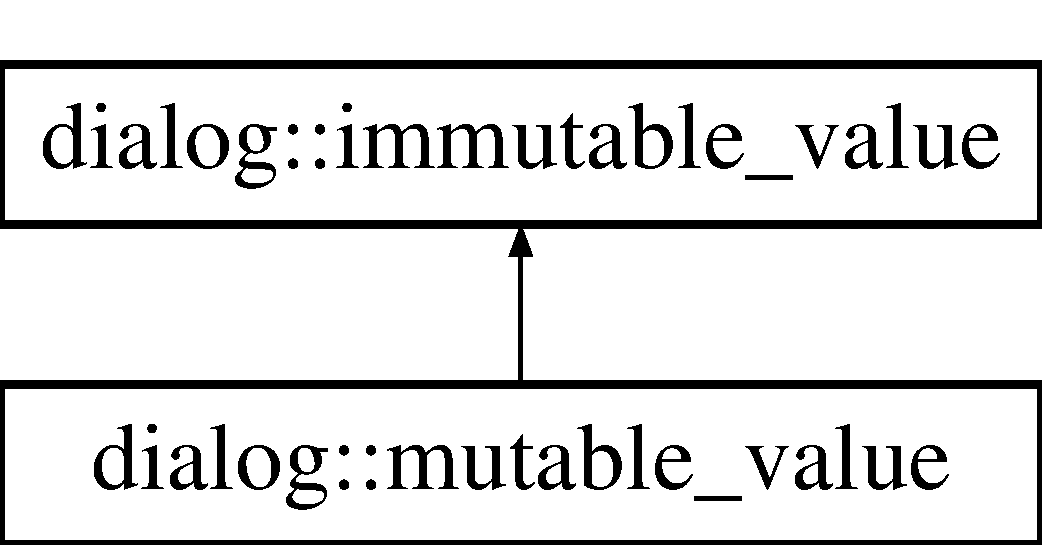
\includegraphics[height=2.000000cm]{classdialog_1_1immutable__value}
\end{center}
\end{figure}
\subsection*{Public Member Functions}
\begin{DoxyCompactItemize}
\item 
\mbox{\Hypertarget{classdialog_1_1immutable__value_a972b2413bb2d99fce071c27416643c42}\label{classdialog_1_1immutable__value_a972b2413bb2d99fce071c27416643c42}} 
{\bfseries immutable\+\_\+value} (const \hyperlink{structdialog_1_1data__type}{data\+\_\+type} \&type=N\+O\+N\+E\+\_\+\+T\+Y\+PE)
\item 
\mbox{\Hypertarget{classdialog_1_1immutable__value_ac0e278c2e032926ba8ebd566b912d8f0}\label{classdialog_1_1immutable__value_ac0e278c2e032926ba8ebd566b912d8f0}} 
{\bfseries immutable\+\_\+value} (const \hyperlink{structdialog_1_1data__type}{data\+\_\+type} \&type, void $\ast$\hyperlink{structdialog_1_1data}{data})
\item 
\mbox{\Hypertarget{classdialog_1_1immutable__value_a3e5010e30ba626c00215f1a79f72ad43}\label{classdialog_1_1immutable__value_a3e5010e30ba626c00215f1a79f72ad43}} 
\hyperlink{structdialog_1_1data__type}{data\+\_\+type} const  \& {\bfseries type} () const
\item 
\mbox{\Hypertarget{classdialog_1_1immutable__value_a2dd1b9b67daf4b11e6fb65e1c472c92c}\label{classdialog_1_1immutable__value_a2dd1b9b67daf4b11e6fb65e1c472c92c}} 
void const  $\ast$ {\bfseries ptr} () const
\item 
\mbox{\Hypertarget{classdialog_1_1immutable__value_a73ff415d17fe3996ab17c58545fe677d}\label{classdialog_1_1immutable__value_a73ff415d17fe3996ab17c58545fe677d}} 
\hyperlink{structdialog_1_1data}{data} {\bfseries to\+\_\+data} () const
\item 
\mbox{\Hypertarget{classdialog_1_1immutable__value_abb8848484b3c749cfc87a5fcb80363d1}\label{classdialog_1_1immutable__value_abb8848484b3c749cfc87a5fcb80363d1}} 
\hyperlink{classdialog_1_1byte__string}{byte\+\_\+string} {\bfseries to\+\_\+key} (double bucket\+\_\+size) const
\item 
\mbox{\Hypertarget{classdialog_1_1immutable__value_ab3506fae357c8e821208377e4233a94c}\label{classdialog_1_1immutable__value_ab3506fae357c8e821208377e4233a94c}} 
{\footnotesize template$<$typename T $>$ }\\T \& {\bfseries as} ()
\item 
\mbox{\Hypertarget{classdialog_1_1immutable__value_a8b80afca630d29dce85d7bdf4b110ad0}\label{classdialog_1_1immutable__value_a8b80afca630d29dce85d7bdf4b110ad0}} 
{\footnotesize template$<$typename T $>$ }\\const T \& {\bfseries as} () const
\item 
\mbox{\Hypertarget{classdialog_1_1immutable__value_abe03c6311a5ff089ce8689efb954dd49}\label{classdialog_1_1immutable__value_abe03c6311a5ff089ce8689efb954dd49}} 
std\+::string {\bfseries to\+\_\+string} () const
\end{DoxyCompactItemize}
\subsection*{Static Public Member Functions}
\begin{DoxyCompactItemize}
\item 
\mbox{\Hypertarget{classdialog_1_1immutable__value_a9df66569c81cb35fff4145e2828fb59b}\label{classdialog_1_1immutable__value_a9df66569c81cb35fff4145e2828fb59b}} 
static bool {\bfseries relop} (relop\+\_\+id id, const \hyperlink{classdialog_1_1immutable__value}{immutable\+\_\+value} \&first, const \hyperlink{classdialog_1_1immutable__value}{immutable\+\_\+value} \&second)
\end{DoxyCompactItemize}
\subsection*{Protected Attributes}
\begin{DoxyCompactItemize}
\item 
\mbox{\Hypertarget{classdialog_1_1immutable__value_a41fee6407da893d330004b5090c13eb7}\label{classdialog_1_1immutable__value_a41fee6407da893d330004b5090c13eb7}} 
\hyperlink{structdialog_1_1data__type}{data\+\_\+type} {\bfseries type\+\_\+}
\item 
\mbox{\Hypertarget{classdialog_1_1immutable__value_ad6b3eb9c03908829677df0eba88445da}\label{classdialog_1_1immutable__value_ad6b3eb9c03908829677df0eba88445da}} 
void $\ast$ {\bfseries ptr\+\_\+}
\end{DoxyCompactItemize}
\subsection*{Friends}
\begin{DoxyCompactItemize}
\item 
\mbox{\Hypertarget{classdialog_1_1immutable__value_a223a5d3f8a4ab47c1a7055ff732f84ac}\label{classdialog_1_1immutable__value_a223a5d3f8a4ab47c1a7055ff732f84ac}} 
bool {\bfseries operator$<$} (const \hyperlink{classdialog_1_1immutable__value}{immutable\+\_\+value} \&first, const \hyperlink{classdialog_1_1immutable__value}{immutable\+\_\+value} \&second)
\item 
\mbox{\Hypertarget{classdialog_1_1immutable__value_ae3747864cc59a8767eb7065a4071ca2c}\label{classdialog_1_1immutable__value_ae3747864cc59a8767eb7065a4071ca2c}} 
bool {\bfseries operator$<$=} (const \hyperlink{classdialog_1_1immutable__value}{immutable\+\_\+value} \&first, const \hyperlink{classdialog_1_1immutable__value}{immutable\+\_\+value} \&second)
\item 
\mbox{\Hypertarget{classdialog_1_1immutable__value_ac9bb357d3f926d85f8d27b06bf86bfa5}\label{classdialog_1_1immutable__value_ac9bb357d3f926d85f8d27b06bf86bfa5}} 
bool {\bfseries operator$>$} (const \hyperlink{classdialog_1_1immutable__value}{immutable\+\_\+value} \&first, const \hyperlink{classdialog_1_1immutable__value}{immutable\+\_\+value} \&second)
\item 
\mbox{\Hypertarget{classdialog_1_1immutable__value_adf272e27a6112206cbe677f5248866d1}\label{classdialog_1_1immutable__value_adf272e27a6112206cbe677f5248866d1}} 
bool {\bfseries operator$>$=} (const \hyperlink{classdialog_1_1immutable__value}{immutable\+\_\+value} \&first, const \hyperlink{classdialog_1_1immutable__value}{immutable\+\_\+value} \&second)
\item 
\mbox{\Hypertarget{classdialog_1_1immutable__value_aafc3d31ba21f46127b6579f33e7d8c2d}\label{classdialog_1_1immutable__value_aafc3d31ba21f46127b6579f33e7d8c2d}} 
bool {\bfseries operator==} (const \hyperlink{classdialog_1_1immutable__value}{immutable\+\_\+value} \&first, const \hyperlink{classdialog_1_1immutable__value}{immutable\+\_\+value} \&second)
\item 
\mbox{\Hypertarget{classdialog_1_1immutable__value_ae99b9a91c1d64387aca36c1b2c1d67b1}\label{classdialog_1_1immutable__value_ae99b9a91c1d64387aca36c1b2c1d67b1}} 
bool {\bfseries operator!=} (const \hyperlink{classdialog_1_1immutable__value}{immutable\+\_\+value} \&first, const \hyperlink{classdialog_1_1immutable__value}{immutable\+\_\+value} \&second)
\end{DoxyCompactItemize}


The documentation for this class was generated from the following file\+:\begin{DoxyCompactItemize}
\item 
/\+Users/neil/\+Documents/\+Berkeley/research/dialog/libdialog/dialog/immutable\+\_\+value.\+h\end{DoxyCompactItemize}

\hypertarget{structdialog_1_1storage_1_1in__memory}{}\section{dialog\+:\+:storage\+:\+:in\+\_\+memory Struct Reference}
\label{structdialog_1_1storage_1_1in__memory}\index{dialog\+::storage\+::in\+\_\+memory@{dialog\+::storage\+::in\+\_\+memory}}


{\ttfamily \#include $<$storage.\+h$>$}

\subsection*{Static Public Member Functions}
\begin{DoxyCompactItemize}
\item 
static void $\ast$ \hyperlink{structdialog_1_1storage_1_1in__memory_a0cf298a53915ebf358d46e864f54ad78}{allocate} (const std\+::string \&path, size\+\_\+t size)
\item 
static void \hyperlink{structdialog_1_1storage_1_1in__memory_af1a8517c282999c0f80fda59de3483d7}{free\+\_\+mem} (void $\ast$ptr, size\+\_\+t size)
\item 
static void \hyperlink{structdialog_1_1storage_1_1in__memory_a8c6edb151f7f3420cb14b567b5c88c64}{flush} (void $\ast$ptr, size\+\_\+t size)
\end{DoxyCompactItemize}


\subsection{Detailed Description}
In memory storage, uses mmap to allocate data that is not backed by a file. 

\subsection{Member Function Documentation}
\mbox{\Hypertarget{structdialog_1_1storage_1_1in__memory_a0cf298a53915ebf358d46e864f54ad78}\label{structdialog_1_1storage_1_1in__memory_a0cf298a53915ebf358d46e864f54ad78}} 
\index{dialog\+::storage\+::in\+\_\+memory@{dialog\+::storage\+::in\+\_\+memory}!allocate@{allocate}}
\index{allocate@{allocate}!dialog\+::storage\+::in\+\_\+memory@{dialog\+::storage\+::in\+\_\+memory}}
\subsubsection{\texorpdfstring{allocate()}{allocate()}}
{\footnotesize\ttfamily static void$\ast$ dialog\+::storage\+::in\+\_\+memory\+::allocate (\begin{DoxyParamCaption}\item[{const std\+::string \&}]{path,  }\item[{size\+\_\+t}]{size }\end{DoxyParamCaption})\hspace{0.3cm}{\ttfamily [inline]}, {\ttfamily [static]}}

Allocates new memory.


\begin{DoxyParams}{Parameters}
{\em path} & Backing file (unused). \\
\hline
{\em size} & Size of requested memory. \\
\hline
\end{DoxyParams}
\mbox{\Hypertarget{structdialog_1_1storage_1_1in__memory_a8c6edb151f7f3420cb14b567b5c88c64}\label{structdialog_1_1storage_1_1in__memory_a8c6edb151f7f3420cb14b567b5c88c64}} 
\index{dialog\+::storage\+::in\+\_\+memory@{dialog\+::storage\+::in\+\_\+memory}!flush@{flush}}
\index{flush@{flush}!dialog\+::storage\+::in\+\_\+memory@{dialog\+::storage\+::in\+\_\+memory}}
\subsubsection{\texorpdfstring{flush()}{flush()}}
{\footnotesize\ttfamily static void dialog\+::storage\+::in\+\_\+memory\+::flush (\begin{DoxyParamCaption}\item[{void $\ast$}]{ptr,  }\item[{size\+\_\+t}]{size }\end{DoxyParamCaption})\hspace{0.3cm}{\ttfamily [inline]}, {\ttfamily [static]}}

Flushes data to backed file (does nothing for this storage mode).


\begin{DoxyParams}{Parameters}
{\em ptr} & Pointer to memory. \\
\hline
{\em size} & Size of allocated memory. \\
\hline
\end{DoxyParams}
\mbox{\Hypertarget{structdialog_1_1storage_1_1in__memory_af1a8517c282999c0f80fda59de3483d7}\label{structdialog_1_1storage_1_1in__memory_af1a8517c282999c0f80fda59de3483d7}} 
\index{dialog\+::storage\+::in\+\_\+memory@{dialog\+::storage\+::in\+\_\+memory}!free\+\_\+mem@{free\+\_\+mem}}
\index{free\+\_\+mem@{free\+\_\+mem}!dialog\+::storage\+::in\+\_\+memory@{dialog\+::storage\+::in\+\_\+memory}}
\subsubsection{\texorpdfstring{free\+\_\+mem()}{free\_mem()}}
{\footnotesize\ttfamily static void dialog\+::storage\+::in\+\_\+memory\+::free\+\_\+mem (\begin{DoxyParamCaption}\item[{void $\ast$}]{ptr,  }\item[{size\+\_\+t}]{size }\end{DoxyParamCaption})\hspace{0.3cm}{\ttfamily [inline]}, {\ttfamily [static]}}

Frees allocated memory.


\begin{DoxyParams}{Parameters}
{\em ptr} & Pointer to memory to be freed. \\
\hline
{\em size} & Size of allocated memory. \\
\hline
\end{DoxyParams}


The documentation for this struct was generated from the following file\+:\begin{DoxyCompactItemize}
\item 
/\+Users/neil/\+Documents/\+Berkeley/research/dialog/libdialog/dialog/storage.\+h\end{DoxyCompactItemize}

\hypertarget{classdialog_1_1index__filter}{}\section{dialog\+:\+:index\+\_\+filter Class Reference}
\label{classdialog_1_1index__filter}\index{dialog\+::index\+\_\+filter@{dialog\+::index\+\_\+filter}}
\subsection*{Public Member Functions}
\begin{DoxyCompactItemize}
\item 
\mbox{\Hypertarget{classdialog_1_1index__filter_a927a410993b0d119be468ef5448b6bbc}\label{classdialog_1_1index__filter_a927a410993b0d119be468ef5448b6bbc}} 
{\bfseries index\+\_\+filter} (uint32\+\_\+t index\+\_\+id, const \hyperlink{classdialog_1_1immutable__byte__string}{immutable\+\_\+byte\+\_\+string} \&key\+\_\+begin, const \hyperlink{classdialog_1_1immutable__byte__string}{immutable\+\_\+byte\+\_\+string} \&key\+\_\+end)
\item 
\mbox{\Hypertarget{classdialog_1_1index__filter_ac75cb858dfbb65d8b60f06e92a984b8e}\label{classdialog_1_1index__filter_ac75cb858dfbb65d8b60f06e92a984b8e}} 
void {\bfseries set\+\_\+keys} (const \hyperlink{classdialog_1_1immutable__byte__string}{immutable\+\_\+byte\+\_\+string} \&begin, const \hyperlink{classdialog_1_1immutable__byte__string}{immutable\+\_\+byte\+\_\+string} \&end)
\item 
\mbox{\Hypertarget{classdialog_1_1index__filter_a28f90c8f53e889211525abb86326341f}\label{classdialog_1_1index__filter_a28f90c8f53e889211525abb86326341f}} 
uint32\+\_\+t {\bfseries index\+\_\+id} () const
\item 
\mbox{\Hypertarget{classdialog_1_1index__filter_addfbf3116860f23652e9a2d9f0fef3f6}\label{classdialog_1_1index__filter_addfbf3116860f23652e9a2d9f0fef3f6}} 
\hyperlink{classdialog_1_1immutable__byte__string}{immutable\+\_\+byte\+\_\+string} const  \& {\bfseries kbegin} () const
\item 
\mbox{\Hypertarget{classdialog_1_1index__filter_a4a8bb0748fedf3db6e8e06dec29f10fe}\label{classdialog_1_1index__filter_a4a8bb0748fedf3db6e8e06dec29f10fe}} 
\hyperlink{classdialog_1_1immutable__byte__string}{immutable\+\_\+byte\+\_\+string} const  \& {\bfseries kend} () const
\item 
\mbox{\Hypertarget{classdialog_1_1index__filter_aee8e4e93802988de1af66e184197c5a3}\label{classdialog_1_1index__filter_aee8e4e93802988de1af66e184197c5a3}} 
std\+::string {\bfseries to\+\_\+string} () const
\end{DoxyCompactItemize}


The documentation for this class was generated from the following file\+:\begin{DoxyCompactItemize}
\item 
/\+Users/neil/\+Documents/\+Berkeley/research/dialog/libdialog/dialog/index\+\_\+filter.\+h\end{DoxyCompactItemize}

\hypertarget{structdialog_1_1index__info}{}\section{dialog\+:\+:index\+\_\+info Struct Reference}
\label{structdialog_1_1index__info}\index{dialog\+::index\+\_\+info@{dialog\+::index\+\_\+info}}
\subsection*{Public Member Functions}
\begin{DoxyCompactItemize}
\item 
\mbox{\Hypertarget{structdialog_1_1index__info_ac65aecab3074cdf5b42121b3e75b71f2}\label{structdialog_1_1index__info_ac65aecab3074cdf5b42121b3e75b71f2}} 
{\bfseries index\+\_\+info} (const std\+::string \&field\+\_\+name, double bucket\+\_\+size)
\item 
\mbox{\Hypertarget{structdialog_1_1index__info_a8a35640303dd8143bd5465368ca5311a}\label{structdialog_1_1index__info_a8a35640303dd8143bd5465368ca5311a}} 
std\+::string {\bfseries field\+\_\+name} () const
\item 
\mbox{\Hypertarget{structdialog_1_1index__info_adc3c71509a3b0b007edbd9a73500c337}\label{structdialog_1_1index__info_adc3c71509a3b0b007edbd9a73500c337}} 
double {\bfseries bucket\+\_\+size} () const
\end{DoxyCompactItemize}


The documentation for this struct was generated from the following file\+:\begin{DoxyCompactItemize}
\item 
/\+Users/neil/\+Documents/\+Berkeley/research/dialog/libdialog/dialog/table\+\_\+metadata.\+h\end{DoxyCompactItemize}

\hypertarget{structdialog_1_1index__state__t}{}\section{dialog\+:\+:index\+\_\+state\+\_\+t Struct Reference}
\label{structdialog_1_1index__state__t}\index{dialog\+::index\+\_\+state\+\_\+t@{dialog\+::index\+\_\+state\+\_\+t}}
\subsection*{Public Member Functions}
\begin{DoxyCompactItemize}
\item 
\mbox{\Hypertarget{structdialog_1_1index__state__t_ac38405add8bd8b66b2928664bdd7c696}\label{structdialog_1_1index__state__t_ac38405add8bd8b66b2928664bdd7c696}} 
{\bfseries index\+\_\+state\+\_\+t} (const \hyperlink{structdialog_1_1index__state__t}{index\+\_\+state\+\_\+t} \&other)
\item 
\mbox{\Hypertarget{structdialog_1_1index__state__t_aff76391ea873aff7d838213b10b21e36}\label{structdialog_1_1index__state__t_aff76391ea873aff7d838213b10b21e36}} 
uint16\+\_\+t {\bfseries id} () const
\item 
\mbox{\Hypertarget{structdialog_1_1index__state__t_ad557a16acaf934c90111dabcc09a07bf}\label{structdialog_1_1index__state__t_ad557a16acaf934c90111dabcc09a07bf}} 
double {\bfseries bucket\+\_\+size} () const
\item 
\mbox{\Hypertarget{structdialog_1_1index__state__t_a6f353cf653f4d775cfbdb8f0f0fff147}\label{structdialog_1_1index__state__t_a6f353cf653f4d775cfbdb8f0f0fff147}} 
\hyperlink{structdialog_1_1index__state__t}{index\+\_\+state\+\_\+t} \& {\bfseries operator=} (const \hyperlink{structdialog_1_1index__state__t}{index\+\_\+state\+\_\+t} \&other)
\item 
\mbox{\Hypertarget{structdialog_1_1index__state__t_a5e49771c6f5cf27ce5b99f04f9c3f1cf}\label{structdialog_1_1index__state__t_a5e49771c6f5cf27ce5b99f04f9c3f1cf}} 
bool {\bfseries is\+\_\+indexed} () const
\item 
\mbox{\Hypertarget{structdialog_1_1index__state__t_ae638a88966b1addedc9ed771261afa21}\label{structdialog_1_1index__state__t_ae638a88966b1addedc9ed771261afa21}} 
bool {\bfseries set\+\_\+indexing} ()
\item 
\mbox{\Hypertarget{structdialog_1_1index__state__t_a2c51ccfb0ca81842091ff050586f80b7}\label{structdialog_1_1index__state__t_a2c51ccfb0ca81842091ff050586f80b7}} 
void {\bfseries set\+\_\+indexed} (uint16\+\_\+t index\+\_\+id, double bucket\+\_\+size)
\item 
\mbox{\Hypertarget{structdialog_1_1index__state__t_a8970c11a3b6bc3324f5f6348b6e52547}\label{structdialog_1_1index__state__t_a8970c11a3b6bc3324f5f6348b6e52547}} 
void {\bfseries set\+\_\+unindexed} ()
\item 
\mbox{\Hypertarget{structdialog_1_1index__state__t_ac2b94de0879937a02049b989993903e9}\label{structdialog_1_1index__state__t_ac2b94de0879937a02049b989993903e9}} 
bool {\bfseries disable\+\_\+indexing} ()
\end{DoxyCompactItemize}
\subsection*{Static Public Attributes}
\begin{DoxyCompactItemize}
\item 
\mbox{\Hypertarget{structdialog_1_1index__state__t_a59650c8c90b9f1768b04a2768c059f3c}\label{structdialog_1_1index__state__t_a59650c8c90b9f1768b04a2768c059f3c}} 
static const uint8\+\_\+t {\bfseries U\+N\+I\+N\+D\+E\+X\+ED} = 0
\item 
\mbox{\Hypertarget{structdialog_1_1index__state__t_a7d689f8e70cb67aa58da7cc74d5addc7}\label{structdialog_1_1index__state__t_a7d689f8e70cb67aa58da7cc74d5addc7}} 
static const uint8\+\_\+t {\bfseries I\+N\+D\+E\+X\+I\+NG} = 1
\item 
\mbox{\Hypertarget{structdialog_1_1index__state__t_a22e470667ecade4e094302c534c3056b}\label{structdialog_1_1index__state__t_a22e470667ecade4e094302c534c3056b}} 
static const uint8\+\_\+t {\bfseries I\+N\+D\+E\+X\+ED} = 2
\end{DoxyCompactItemize}


The documentation for this struct was generated from the following file\+:\begin{DoxyCompactItemize}
\item 
/\+Users/neil/\+Documents/\+Berkeley/research/dialog/libdialog/dialog/index\+\_\+state.\+h\end{DoxyCompactItemize}

\hypertarget{classdialog_1_1index_1_1indexlet}{}\section{dialog\+:\+:index\+:\+:indexlet$<$ T, S\+I\+ZE $>$ Class Template Reference}
\label{classdialog_1_1index_1_1indexlet}\index{dialog\+::index\+::indexlet$<$ T, S\+I\+Z\+E $>$@{dialog\+::index\+::indexlet$<$ T, S\+I\+Z\+E $>$}}


The unit of indexing in tiered indexes.  




{\ttfamily \#include $<$tiered\+\_\+index.\+h$>$}

\subsection*{Public Types}
\begin{DoxyCompactItemize}
\item 
\mbox{\Hypertarget{classdialog_1_1index_1_1indexlet_ae0261936539a2e33e07319981977dda3}\label{classdialog_1_1index_1_1indexlet_ae0261936539a2e33e07319981977dda3}} 
typedef atomic\+::type$<$ T $\ast$ $>$ {\bfseries atomic\+\_\+ref}
\end{DoxyCompactItemize}
\subsection*{Public Member Functions}
\begin{DoxyCompactItemize}
\item 
\hyperlink{classdialog_1_1index_1_1indexlet_ab1bb4556decdfc358090e73a078e45d2}{indexlet} ()
\begin{DoxyCompactList}\small\item\em Constructor for the indexlet. \end{DoxyCompactList}\item 
virtual \hyperlink{classdialog_1_1index_1_1indexlet_afada63e2f9ead60d701688a06c2fcd81}{$\sim$indexlet} ()
\begin{DoxyCompactList}\small\item\em Virtual destructor for indexlet. \end{DoxyCompactList}\item 
T $\ast$ \hyperlink{classdialog_1_1index_1_1indexlet_aac4ccc3e9c4aa70bfebac6f8b48de7eb}{get\+\_\+or\+\_\+create} (const uint32\+\_\+t i)
\begin{DoxyCompactList}\small\item\em Creates and fetches the value at a given index. \end{DoxyCompactList}\item 
atomic\+\_\+ref $\ast$ \hyperlink{classdialog_1_1index_1_1indexlet_ab3d280e9176781621a9b9c627c7db0e6}{get\+\_\+atomic} (const uint32\+\_\+t i)
\begin{DoxyCompactList}\small\item\em Fetches the atomic pointer at a given index. \end{DoxyCompactList}\item 
T $\ast$ \hyperlink{classdialog_1_1index_1_1indexlet_a879de6014445e5fdd8091a8f20ced31a}{operator\mbox{[}$\,$\mbox{]}} (const uint32\+\_\+t i)
\begin{DoxyCompactList}\small\item\em Operator override for accessing the value at a given index. \end{DoxyCompactList}\item 
T $\ast$ \hyperlink{classdialog_1_1index_1_1indexlet_a06b8f0bb16c6ffc2ab1c13404d099298}{get} (const uint32\+\_\+t i) const
\begin{DoxyCompactList}\small\item\em Function for getting the value at a given index. \end{DoxyCompactList}\item 
size\+\_\+t \hyperlink{classdialog_1_1index_1_1indexlet_ade4239f0aba692226fb8dd9ff899df87}{size} ()
\begin{DoxyCompactList}\small\item\em Get the size of the indexlet. \end{DoxyCompactList}\item 
size\+\_\+t \hyperlink{classdialog_1_1index_1_1indexlet_a68a3f311fb6b2172c70619bc633e729b}{storage\+\_\+size} ()
\begin{DoxyCompactList}\small\item\em Get the storage size in bytes of the indexlet. \end{DoxyCompactList}\end{DoxyCompactItemize}


\subsection{Detailed Description}
\subsubsection*{template$<$typename T, size\+\_\+t S\+I\+ZE = 65536$>$\newline
class dialog\+::index\+::indexlet$<$ T, S\+I\+Z\+E $>$}

The unit of indexing in tiered indexes. 

The basic unit of indexing in tiered indexes. An indexlet stores a fixed-\/size array with atomic references to objects of value type.


\begin{DoxyTemplParams}{Template Parameters}
{\em T} & Tyepe of the value. \\
\hline
{\em S\+I\+ZE} & = 65536 Size of the fixed-\/size array. \\
\hline
\end{DoxyTemplParams}


\subsection{Constructor \& Destructor Documentation}
\mbox{\Hypertarget{classdialog_1_1index_1_1indexlet_ab1bb4556decdfc358090e73a078e45d2}\label{classdialog_1_1index_1_1indexlet_ab1bb4556decdfc358090e73a078e45d2}} 
\index{dialog\+::index\+::indexlet@{dialog\+::index\+::indexlet}!indexlet@{indexlet}}
\index{indexlet@{indexlet}!dialog\+::index\+::indexlet@{dialog\+::index\+::indexlet}}
\subsubsection{\texorpdfstring{indexlet()}{indexlet()}}
{\footnotesize\ttfamily template$<$typename T, size\+\_\+t S\+I\+ZE = 65536$>$ \\
\hyperlink{classdialog_1_1index_1_1indexlet}{dialog\+::index\+::indexlet}$<$ T, S\+I\+ZE $>$\+::\hyperlink{classdialog_1_1index_1_1indexlet}{indexlet} (\begin{DoxyParamCaption}{ }\end{DoxyParamCaption})\hspace{0.3cm}{\ttfamily [inline]}}



Constructor for the indexlet. 

Constructor for the indexlet. Initializes all array references to null. \mbox{\Hypertarget{classdialog_1_1index_1_1indexlet_afada63e2f9ead60d701688a06c2fcd81}\label{classdialog_1_1index_1_1indexlet_afada63e2f9ead60d701688a06c2fcd81}} 
\index{dialog\+::index\+::indexlet@{dialog\+::index\+::indexlet}!````~indexlet@{$\sim$indexlet}}
\index{````~indexlet@{$\sim$indexlet}!dialog\+::index\+::indexlet@{dialog\+::index\+::indexlet}}
\subsubsection{\texorpdfstring{$\sim$indexlet()}{~indexlet()}}
{\footnotesize\ttfamily template$<$typename T, size\+\_\+t S\+I\+ZE = 65536$>$ \\
virtual \hyperlink{classdialog_1_1index_1_1indexlet}{dialog\+::index\+::indexlet}$<$ T, S\+I\+ZE $>$\+::$\sim$\hyperlink{classdialog_1_1index_1_1indexlet}{indexlet} (\begin{DoxyParamCaption}{ }\end{DoxyParamCaption})\hspace{0.3cm}{\ttfamily [inline]}, {\ttfamily [virtual]}}



Virtual destructor for indexlet. 

Virtual destructor for indexlet. Deletes all array references. 

\subsection{Member Function Documentation}
\mbox{\Hypertarget{classdialog_1_1index_1_1indexlet_a06b8f0bb16c6ffc2ab1c13404d099298}\label{classdialog_1_1index_1_1indexlet_a06b8f0bb16c6ffc2ab1c13404d099298}} 
\index{dialog\+::index\+::indexlet@{dialog\+::index\+::indexlet}!get@{get}}
\index{get@{get}!dialog\+::index\+::indexlet@{dialog\+::index\+::indexlet}}
\subsubsection{\texorpdfstring{get()}{get()}}
{\footnotesize\ttfamily template$<$typename T, size\+\_\+t S\+I\+ZE = 65536$>$ \\
T$\ast$ \hyperlink{classdialog_1_1index_1_1indexlet}{dialog\+::index\+::indexlet}$<$ T, S\+I\+ZE $>$\+::get (\begin{DoxyParamCaption}\item[{const uint32\+\_\+t}]{i }\end{DoxyParamCaption}) const\hspace{0.3cm}{\ttfamily [inline]}}



Function for getting the value at a given index. 

Function for getting the value at a given index.


\begin{DoxyParams}{Parameters}
{\em i} & The index to lookup. \\
\hline
\end{DoxyParams}
\begin{DoxyReturn}{Returns}
Pointer to the value. 
\end{DoxyReturn}
\mbox{\Hypertarget{classdialog_1_1index_1_1indexlet_ab3d280e9176781621a9b9c627c7db0e6}\label{classdialog_1_1index_1_1indexlet_ab3d280e9176781621a9b9c627c7db0e6}} 
\index{dialog\+::index\+::indexlet@{dialog\+::index\+::indexlet}!get\+\_\+atomic@{get\+\_\+atomic}}
\index{get\+\_\+atomic@{get\+\_\+atomic}!dialog\+::index\+::indexlet@{dialog\+::index\+::indexlet}}
\subsubsection{\texorpdfstring{get\+\_\+atomic()}{get\_atomic()}}
{\footnotesize\ttfamily template$<$typename T, size\+\_\+t S\+I\+ZE = 65536$>$ \\
atomic\+\_\+ref$\ast$ \hyperlink{classdialog_1_1index_1_1indexlet}{dialog\+::index\+::indexlet}$<$ T, S\+I\+ZE $>$\+::get\+\_\+atomic (\begin{DoxyParamCaption}\item[{const uint32\+\_\+t}]{i }\end{DoxyParamCaption})\hspace{0.3cm}{\ttfamily [inline]}}



Fetches the atomic pointer at a given index. 

Obtain the atomic pointer at a given index.


\begin{DoxyParams}{Parameters}
{\em i} & The index to lookup. \\
\hline
\end{DoxyParams}
\begin{DoxyReturn}{Returns}
Atomic pointer to the value. 
\end{DoxyReturn}
\mbox{\Hypertarget{classdialog_1_1index_1_1indexlet_aac4ccc3e9c4aa70bfebac6f8b48de7eb}\label{classdialog_1_1index_1_1indexlet_aac4ccc3e9c4aa70bfebac6f8b48de7eb}} 
\index{dialog\+::index\+::indexlet@{dialog\+::index\+::indexlet}!get\+\_\+or\+\_\+create@{get\+\_\+or\+\_\+create}}
\index{get\+\_\+or\+\_\+create@{get\+\_\+or\+\_\+create}!dialog\+::index\+::indexlet@{dialog\+::index\+::indexlet}}
\subsubsection{\texorpdfstring{get\+\_\+or\+\_\+create()}{get\_or\_create()}}
{\footnotesize\ttfamily template$<$typename T, size\+\_\+t S\+I\+ZE = 65536$>$ \\
T$\ast$ \hyperlink{classdialog_1_1index_1_1indexlet}{dialog\+::index\+::indexlet}$<$ T, S\+I\+ZE $>$\+::get\+\_\+or\+\_\+create (\begin{DoxyParamCaption}\item[{const uint32\+\_\+t}]{i }\end{DoxyParamCaption})\hspace{0.3cm}{\ttfamily [inline]}}



Creates and fetches the value at a given index. 

Obtain the value at a given index; creates required internal structure for the value if it does not exist.


\begin{DoxyParams}{Parameters}
{\em i} & The index to lookup. \\
\hline
\end{DoxyParams}
\begin{DoxyReturn}{Returns}
Pointer to the value. 
\end{DoxyReturn}
\mbox{\Hypertarget{classdialog_1_1index_1_1indexlet_a879de6014445e5fdd8091a8f20ced31a}\label{classdialog_1_1index_1_1indexlet_a879de6014445e5fdd8091a8f20ced31a}} 
\index{dialog\+::index\+::indexlet@{dialog\+::index\+::indexlet}!operator\mbox{[}\mbox{]}@{operator[]}}
\index{operator\mbox{[}\mbox{]}@{operator[]}!dialog\+::index\+::indexlet@{dialog\+::index\+::indexlet}}
\subsubsection{\texorpdfstring{operator[]()}{operator[]()}}
{\footnotesize\ttfamily template$<$typename T, size\+\_\+t S\+I\+ZE = 65536$>$ \\
T$\ast$ \hyperlink{classdialog_1_1index_1_1indexlet}{dialog\+::index\+::indexlet}$<$ T, S\+I\+ZE $>$\+::operator\mbox{[}$\,$\mbox{]} (\begin{DoxyParamCaption}\item[{const uint32\+\_\+t}]{i }\end{DoxyParamCaption})\hspace{0.3cm}{\ttfamily [inline]}}



Operator override for accessing the value at a given index. 

Overrides operator for accessing accessing the value at a given index. Creates any required internal structure.


\begin{DoxyParams}{Parameters}
{\em i} & Index of the value. \\
\hline
\end{DoxyParams}
\mbox{\Hypertarget{classdialog_1_1index_1_1indexlet_ade4239f0aba692226fb8dd9ff899df87}\label{classdialog_1_1index_1_1indexlet_ade4239f0aba692226fb8dd9ff899df87}} 
\index{dialog\+::index\+::indexlet@{dialog\+::index\+::indexlet}!size@{size}}
\index{size@{size}!dialog\+::index\+::indexlet@{dialog\+::index\+::indexlet}}
\subsubsection{\texorpdfstring{size()}{size()}}
{\footnotesize\ttfamily template$<$typename T, size\+\_\+t S\+I\+ZE = 65536$>$ \\
size\+\_\+t \hyperlink{classdialog_1_1index_1_1indexlet}{dialog\+::index\+::indexlet}$<$ T, S\+I\+ZE $>$\+::size (\begin{DoxyParamCaption}{ }\end{DoxyParamCaption})\hspace{0.3cm}{\ttfamily [inline]}}



Get the size of the indexlet. 

Get the size of the indexlet. \begin{DoxyReturn}{Returns}
Size of the indexlet. 
\end{DoxyReturn}
\mbox{\Hypertarget{classdialog_1_1index_1_1indexlet_a68a3f311fb6b2172c70619bc633e729b}\label{classdialog_1_1index_1_1indexlet_a68a3f311fb6b2172c70619bc633e729b}} 
\index{dialog\+::index\+::indexlet@{dialog\+::index\+::indexlet}!storage\+\_\+size@{storage\+\_\+size}}
\index{storage\+\_\+size@{storage\+\_\+size}!dialog\+::index\+::indexlet@{dialog\+::index\+::indexlet}}
\subsubsection{\texorpdfstring{storage\+\_\+size()}{storage\_size()}}
{\footnotesize\ttfamily template$<$typename T, size\+\_\+t S\+I\+ZE = 65536$>$ \\
size\+\_\+t \hyperlink{classdialog_1_1index_1_1indexlet}{dialog\+::index\+::indexlet}$<$ T, S\+I\+ZE $>$\+::storage\+\_\+size (\begin{DoxyParamCaption}{ }\end{DoxyParamCaption})\hspace{0.3cm}{\ttfamily [inline]}}



Get the storage size in bytes of the indexlet. 

Get the storage size in bytes of the indexlet. \begin{DoxyReturn}{Returns}
The storage size in bytes of the indexlet. 
\end{DoxyReturn}


The documentation for this class was generated from the following file\+:\begin{DoxyCompactItemize}
\item 
/\+Users/neil/\+Documents/\+Berkeley/research/dialog/libdialog/dialog/tiered\+\_\+index.\+h\end{DoxyCompactItemize}

\hypertarget{structdialog_1_1string__map_1_1map__entry}{}\section{dialog\+:\+:string\+\_\+map$<$ V $>$\+:\+:map\+\_\+entry Struct Reference}
\label{structdialog_1_1string__map_1_1map__entry}\index{dialog\+::string\+\_\+map$<$ V $>$\+::map\+\_\+entry@{dialog\+::string\+\_\+map$<$ V $>$\+::map\+\_\+entry}}
\subsection*{Public Member Functions}
\begin{DoxyCompactItemize}
\item 
\mbox{\Hypertarget{structdialog_1_1string__map_1_1map__entry_ad4da6a1dace8b9606589ec4eaa6793e0}\label{structdialog_1_1string__map_1_1map__entry_ad4da6a1dace8b9606589ec4eaa6793e0}} 
{\bfseries map\+\_\+entry} (const std\+::string \&k, const V \&v)
\end{DoxyCompactItemize}
\subsection*{Public Attributes}
\begin{DoxyCompactItemize}
\item 
\mbox{\Hypertarget{structdialog_1_1string__map_1_1map__entry_a4f0528ab94efa27c499f3fdbf3721371}\label{structdialog_1_1string__map_1_1map__entry_a4f0528ab94efa27c499f3fdbf3721371}} 
std\+::string {\bfseries key}
\item 
\mbox{\Hypertarget{structdialog_1_1string__map_1_1map__entry_ac6f877850d9c7c41b4f2e5e631dd4245}\label{structdialog_1_1string__map_1_1map__entry_ac6f877850d9c7c41b4f2e5e631dd4245}} 
V {\bfseries value}
\item 
\mbox{\Hypertarget{structdialog_1_1string__map_1_1map__entry_a8efec7d687e3d9194f27f4a8300cb775}\label{structdialog_1_1string__map_1_1map__entry_a8efec7d687e3d9194f27f4a8300cb775}} 
bool {\bfseries valid}
\end{DoxyCompactItemize}


The documentation for this struct was generated from the following file\+:\begin{DoxyCompactItemize}
\item 
/\+Users/neil/\+Documents/\+Berkeley/research/dialog/libdialog/dialog/string\+\_\+map.\+h\end{DoxyCompactItemize}

\hypertarget{structdialog_1_1marked__ptr}{}\section{dialog\+:\+:marked\+\_\+ptr$<$ T $>$ Struct Template Reference}
\label{structdialog_1_1marked__ptr}\index{dialog\+::marked\+\_\+ptr$<$ T $>$@{dialog\+::marked\+\_\+ptr$<$ T $>$}}
\subsection*{Public Member Functions}
\begin{DoxyCompactItemize}
\item 
\mbox{\Hypertarget{structdialog_1_1marked__ptr_a0c5cb3ea7df17617e8eb36125caad9a2}\label{structdialog_1_1marked__ptr_a0c5cb3ea7df17617e8eb36125caad9a2}} 
{\bfseries marked\+\_\+ptr} (bool mark, uintptr\+\_\+t ptr)
\item 
\mbox{\Hypertarget{structdialog_1_1marked__ptr_a3a8c6534187e6aaf26eb1ae14e7ceeea}\label{structdialog_1_1marked__ptr_a3a8c6534187e6aaf26eb1ae14e7ceeea}} 
bool {\bfseries is\+\_\+marked} () const
\item 
\mbox{\Hypertarget{structdialog_1_1marked__ptr_ae2805da3106dbb27901736c92c1e4731}\label{structdialog_1_1marked__ptr_ae2805da3106dbb27901736c92c1e4731}} 
T \& {\bfseries operator$\ast$} ()
\item 
\mbox{\Hypertarget{structdialog_1_1marked__ptr_aa34bbb2dc822861452b9bc91dbec7830}\label{structdialog_1_1marked__ptr_aa34bbb2dc822861452b9bc91dbec7830}} 
T $\ast$ {\bfseries operator-\/$>$} ()
\item 
\mbox{\Hypertarget{structdialog_1_1marked__ptr_ac09bcb689595c6bc3f3dda12e8b591e7}\label{structdialog_1_1marked__ptr_ac09bcb689595c6bc3f3dda12e8b591e7}} 
T $\ast$ {\bfseries ptr} () const
\item 
\mbox{\Hypertarget{structdialog_1_1marked__ptr_ad8010102e1d52322c4991b6425b59bf2}\label{structdialog_1_1marked__ptr_ad8010102e1d52322c4991b6425b59bf2}} 
bool {\bfseries operator==} (const \hyperlink{structdialog_1_1marked__ptr}{marked\+\_\+ptr}$<$ T $>$ \&other) const
\item 
\mbox{\Hypertarget{structdialog_1_1marked__ptr_a6c2089f165d66213f936a05adf417874}\label{structdialog_1_1marked__ptr_a6c2089f165d66213f936a05adf417874}} 
bool {\bfseries operator!=} (const \hyperlink{structdialog_1_1marked__ptr}{marked\+\_\+ptr}$<$ T $>$ \&other) const
\item 
\mbox{\Hypertarget{structdialog_1_1marked__ptr_adc31b51e967006e2c856bb2f13eff68c}\label{structdialog_1_1marked__ptr_adc31b51e967006e2c856bb2f13eff68c}} 
\hyperlink{structdialog_1_1marked__ptr}{marked\+\_\+ptr}$<$ T $>$ {\bfseries unmarked} () const
\item 
\mbox{\Hypertarget{structdialog_1_1marked__ptr_a772a3106d4a350399d2c4324b1361f45}\label{structdialog_1_1marked__ptr_a772a3106d4a350399d2c4324b1361f45}} 
\hyperlink{structdialog_1_1marked__ptr}{marked\+\_\+ptr}$<$ T $>$ {\bfseries marked} () const
\item 
\mbox{\Hypertarget{structdialog_1_1marked__ptr_aeecc5639da1c80844fbc85a72254f6ad}\label{structdialog_1_1marked__ptr_aeecc5639da1c80844fbc85a72254f6ad}} 
bool {\bfseries is\+\_\+uninitialized} () const
\end{DoxyCompactItemize}


The documentation for this struct was generated from the following file\+:\begin{DoxyCompactItemize}
\item 
/\+Users/neil/\+Documents/\+Berkeley/research/dialog/libdialog/dialog/searchable\+\_\+list.\+h\end{DoxyCompactItemize}

\hypertarget{classdialog_1_1metadata__reader}{}\section{dialog\+:\+:metadata\+\_\+reader Class Reference}
\label{classdialog_1_1metadata__reader}\index{dialog\+::metadata\+\_\+reader@{dialog\+::metadata\+\_\+reader}}
\subsection*{Public Member Functions}
\begin{DoxyCompactItemize}
\item 
\mbox{\Hypertarget{classdialog_1_1metadata__reader_a1c24163850b7540c5381396d1d06d485}\label{classdialog_1_1metadata__reader_a1c24163850b7540c5381396d1d06d485}} 
{\bfseries metadata\+\_\+reader} (const std\+::string \&path)
\item 
\mbox{\Hypertarget{classdialog_1_1metadata__reader_aaf29d7875368ca3b5d7e13d3609e858b}\label{classdialog_1_1metadata__reader_aaf29d7875368ca3b5d7e13d3609e858b}} 
metadata\+\_\+type {\bfseries next\+\_\+type} ()
\item 
\mbox{\Hypertarget{classdialog_1_1metadata__reader_a6f30d4bbfb267e091ad6f2a54327e4b1}\label{classdialog_1_1metadata__reader_a6f30d4bbfb267e091ad6f2a54327e4b1}} 
\hyperlink{classdialog_1_1schema__t}{schema\+\_\+t} {\bfseries next\+\_\+schema} ()
\item 
\mbox{\Hypertarget{classdialog_1_1metadata__reader_a8df956689df5101f445e074de62f7f0b}\label{classdialog_1_1metadata__reader_a8df956689df5101f445e074de62f7f0b}} 
\hyperlink{structdialog_1_1index__info}{index\+\_\+info} {\bfseries next\+\_\+index\+\_\+info} ()
\item 
\mbox{\Hypertarget{classdialog_1_1metadata__reader_a9e0eb82c6918326dce0d7f58be48eb45}\label{classdialog_1_1metadata__reader_a9e0eb82c6918326dce0d7f58be48eb45}} 
\hyperlink{structdialog_1_1filter__info}{filter\+\_\+info} {\bfseries next\+\_\+filter\+\_\+info} ()
\item 
\mbox{\Hypertarget{classdialog_1_1metadata__reader_ae2d0c17b8876e1286d16a6d01d22fc99}\label{classdialog_1_1metadata__reader_ae2d0c17b8876e1286d16a6d01d22fc99}} 
\hyperlink{structdialog_1_1trigger__info}{trigger\+\_\+info} {\bfseries next\+\_\+trigger\+\_\+info} ()
\end{DoxyCompactItemize}


The documentation for this class was generated from the following file\+:\begin{DoxyCompactItemize}
\item 
/\+Users/neil/\+Documents/\+Berkeley/research/dialog/libdialog/dialog/table\+\_\+metadata.\+h\end{DoxyCompactItemize}

\hypertarget{classdialog_1_1metadata__writer}{}\section{dialog\+:\+:metadata\+\_\+writer Class Reference}
\label{classdialog_1_1metadata__writer}\index{dialog\+::metadata\+\_\+writer@{dialog\+::metadata\+\_\+writer}}
\subsection*{Public Member Functions}
\begin{DoxyCompactItemize}
\item 
\mbox{\Hypertarget{classdialog_1_1metadata__writer_a0d15f0dfbedada257e6cd823f45a5549}\label{classdialog_1_1metadata__writer_a0d15f0dfbedada257e6cd823f45a5549}} 
{\bfseries metadata\+\_\+writer} (const std\+::string \&path, storage\+::storage\+\_\+id id)
\item 
\mbox{\Hypertarget{classdialog_1_1metadata__writer_aa2afdab72496ce667cdc152e84bf6d4b}\label{classdialog_1_1metadata__writer_aa2afdab72496ce667cdc152e84bf6d4b}} 
void {\bfseries write\+\_\+schema} (const \hyperlink{classdialog_1_1schema__t}{schema\+\_\+t} \&schema)
\item 
\mbox{\Hypertarget{classdialog_1_1metadata__writer_a4e637156b29bdfcb043780d2fa305e11}\label{classdialog_1_1metadata__writer_a4e637156b29bdfcb043780d2fa305e11}} 
void {\bfseries write\+\_\+index\+\_\+info} (const std\+::string \&name, double bucket\+\_\+size)
\item 
\mbox{\Hypertarget{classdialog_1_1metadata__writer_ad0e4dada645536bcdb364b32ce515223}\label{classdialog_1_1metadata__writer_ad0e4dada645536bcdb364b32ce515223}} 
void {\bfseries write\+\_\+filter\+\_\+info} (const std\+::string \&filter\+\_\+name, const std\+::string \&expr)
\item 
\mbox{\Hypertarget{classdialog_1_1metadata__writer_ab7fc38445852d6694a29eb3517c8cc10}\label{classdialog_1_1metadata__writer_ab7fc38445852d6694a29eb3517c8cc10}} 
void {\bfseries write\+\_\+trigger\+\_\+info} (const std\+::string \&trigger\+\_\+name, const std\+::string \&filter\+\_\+name, aggregate\+\_\+id agg\+\_\+id, const std\+::string \&field\+\_\+name, relop\+\_\+id op, const \hyperlink{classdialog_1_1numeric}{numeric} \&threshold)
\end{DoxyCompactItemize}


The documentation for this class was generated from the following file\+:\begin{DoxyCompactItemize}
\item 
/\+Users/neil/\+Documents/\+Berkeley/research/dialog/libdialog/dialog/table\+\_\+metadata.\+h\end{DoxyCompactItemize}

\hypertarget{classdialog_1_1minterm__plan}{}\section{dialog\+:\+:minterm\+\_\+plan Class Reference}
\label{classdialog_1_1minterm__plan}\index{dialog\+::minterm\+\_\+plan@{dialog\+::minterm\+\_\+plan}}
\subsection*{Public Member Functions}
\begin{DoxyCompactItemize}
\item 
\hyperlink{classdialog_1_1minterm__plan_a547b1de0f11a8ac86b78d5f4ce705e40}{minterm\+\_\+plan} (const \hyperlink{classdialog_1_1index__filter}{index\+\_\+filter} \&ifilter, const \hyperlink{structdialog_1_1compiled__minterm}{compiled\+\_\+minterm} \&dfilter)
\item 
\mbox{\Hypertarget{classdialog_1_1minterm__plan_a13c39f09e13a13780fa3fad2705166c9}\label{classdialog_1_1minterm__plan_a13c39f09e13a13780fa3fad2705166c9}} 
\hyperlink{classdialog_1_1index__filter}{index\+\_\+filter} const  \& {\bfseries idx\+\_\+filter} () const
\item 
\mbox{\Hypertarget{classdialog_1_1minterm__plan_a2d069c2597da15711483acfe8a0b9cfc}\label{classdialog_1_1minterm__plan_a2d069c2597da15711483acfe8a0b9cfc}} 
\hyperlink{structdialog_1_1compiled__expression}{compiled\+\_\+expression} const  \& {\bfseries data\+\_\+filter} () const
\item 
\mbox{\Hypertarget{classdialog_1_1minterm__plan_a2ea3335284edcf3db9727b1acb8ec108}\label{classdialog_1_1minterm__plan_a2ea3335284edcf3db9727b1acb8ec108}} 
std\+::string {\bfseries to\+\_\+string} () const
\end{DoxyCompactItemize}


\subsection{Constructor \& Destructor Documentation}
\mbox{\Hypertarget{classdialog_1_1minterm__plan_a547b1de0f11a8ac86b78d5f4ce705e40}\label{classdialog_1_1minterm__plan_a547b1de0f11a8ac86b78d5f4ce705e40}} 
\index{dialog\+::minterm\+\_\+plan@{dialog\+::minterm\+\_\+plan}!minterm\+\_\+plan@{minterm\+\_\+plan}}
\index{minterm\+\_\+plan@{minterm\+\_\+plan}!dialog\+::minterm\+\_\+plan@{dialog\+::minterm\+\_\+plan}}
\subsubsection{\texorpdfstring{minterm\+\_\+plan()}{minterm\_plan()}}
{\footnotesize\ttfamily dialog\+::minterm\+\_\+plan\+::minterm\+\_\+plan (\begin{DoxyParamCaption}\item[{const \hyperlink{classdialog_1_1index__filter}{index\+\_\+filter} \&}]{ifilter,  }\item[{const \hyperlink{structdialog_1_1compiled__minterm}{compiled\+\_\+minterm} \&}]{dfilter }\end{DoxyParamCaption})\hspace{0.3cm}{\ttfamily [inline]}}

Constructor for the minterm 
\begin{DoxyParams}{Parameters}
{\em ifilter} & The index filter for the \\
\hline
\end{DoxyParams}


The documentation for this class was generated from the following file\+:\begin{DoxyCompactItemize}
\item 
/\+Users/neil/\+Documents/\+Berkeley/research/dialog/libdialog/dialog/query\+\_\+plan.\+h\end{DoxyCompactItemize}

\hypertarget{classdialog_1_1monolog_1_1monolog__block}{}\section{dialog\+:\+:monolog\+:\+:monolog\+\_\+block$<$ T, B\+U\+F\+F\+E\+R\+\_\+\+S\+I\+ZE $>$ Class Template Reference}
\label{classdialog_1_1monolog_1_1monolog__block}\index{dialog\+::monolog\+::monolog\+\_\+block$<$ T, B\+U\+F\+F\+E\+R\+\_\+\+S\+I\+Z\+E $>$@{dialog\+::monolog\+::monolog\+\_\+block$<$ T, B\+U\+F\+F\+E\+R\+\_\+\+S\+I\+Z\+E $>$}}
\subsection*{Public Types}
\begin{DoxyCompactItemize}
\item 
\mbox{\Hypertarget{classdialog_1_1monolog_1_1monolog__block_ab4e944acf2c4accd9063fb5955cd9c1b}\label{classdialog_1_1monolog_1_1monolog__block_ab4e944acf2c4accd9063fb5955cd9c1b}} 
typedef bool {\bfseries block\+\_\+state}
\end{DoxyCompactItemize}
\subsection*{Public Member Functions}
\begin{DoxyCompactItemize}
\item 
\mbox{\Hypertarget{classdialog_1_1monolog_1_1monolog__block_a8d913e738c1038d194493afabd5a163a}\label{classdialog_1_1monolog_1_1monolog__block_a8d913e738c1038d194493afabd5a163a}} 
{\bfseries monolog\+\_\+block} (const std\+::string \&path, size\+\_\+t size, const \hyperlink{structdialog_1_1storage_1_1storage__mode}{storage\+::storage\+\_\+mode} \&storage)
\item 
\mbox{\Hypertarget{classdialog_1_1monolog_1_1monolog__block_ac62dbe270684c1913ecfbe6c4ffc2106}\label{classdialog_1_1monolog_1_1monolog__block_ac62dbe270684c1913ecfbe6c4ffc2106}} 
{\bfseries monolog\+\_\+block} (const \hyperlink{classdialog_1_1monolog_1_1monolog__block}{monolog\+\_\+block} \&other)
\item 
\mbox{\Hypertarget{classdialog_1_1monolog_1_1monolog__block_a60c7dc093c2168365a13436b1c8232ae}\label{classdialog_1_1monolog_1_1monolog__block_a60c7dc093c2168365a13436b1c8232ae}} 
void {\bfseries init} (const std\+::string \&path, const size\+\_\+t size, const \hyperlink{structdialog_1_1storage_1_1storage__mode}{storage\+::storage\+\_\+mode} \&storage)
\item 
\mbox{\Hypertarget{classdialog_1_1monolog_1_1monolog__block_ae62550c498712643d68cebac4fcc2dbd}\label{classdialog_1_1monolog_1_1monolog__block_ae62550c498712643d68cebac4fcc2dbd}} 
size\+\_\+t {\bfseries storage\+\_\+size} () const
\item 
\mbox{\Hypertarget{classdialog_1_1monolog_1_1monolog__block_a011e51ee79e69a714a54846f4faac934}\label{classdialog_1_1monolog_1_1monolog__block_a011e51ee79e69a714a54846f4faac934}} 
void {\bfseries flush} (size\+\_\+t offset, size\+\_\+t len)
\item 
\mbox{\Hypertarget{classdialog_1_1monolog_1_1monolog__block_a848fc37d24b99a125b314ed00d4e9ed3}\label{classdialog_1_1monolog_1_1monolog__block_a848fc37d24b99a125b314ed00d4e9ed3}} 
void {\bfseries set} (size\+\_\+t i, const T \&val)
\item 
\mbox{\Hypertarget{classdialog_1_1monolog_1_1monolog__block_abd7d20244b68a05ac9f5d9bdf42e0255}\label{classdialog_1_1monolog_1_1monolog__block_abd7d20244b68a05ac9f5d9bdf42e0255}} 
void {\bfseries set\+\_\+unsafe} (size\+\_\+t i, const T \&val)
\item 
\mbox{\Hypertarget{classdialog_1_1monolog_1_1monolog__block_ad5e410b9dde8f44a1960e87beade503c}\label{classdialog_1_1monolog_1_1monolog__block_ad5e410b9dde8f44a1960e87beade503c}} 
void {\bfseries write} (size\+\_\+t offset, const T $\ast$\hyperlink{structdialog_1_1data}{data}, size\+\_\+t len)
\item 
\mbox{\Hypertarget{classdialog_1_1monolog_1_1monolog__block_ac4697bb76d9e298c3444c174c51a0f76}\label{classdialog_1_1monolog_1_1monolog__block_ac4697bb76d9e298c3444c174c51a0f76}} 
void {\bfseries write\+\_\+unsafe} (size\+\_\+t offset, const T $\ast$\hyperlink{structdialog_1_1data}{data}, size\+\_\+t len)
\item 
\mbox{\Hypertarget{classdialog_1_1monolog_1_1monolog__block_afd735c98a1a3b35a0c0edefa29698163}\label{classdialog_1_1monolog_1_1monolog__block_afd735c98a1a3b35a0c0edefa29698163}} 
const T \& {\bfseries at} (size\+\_\+t i) const
\item 
\mbox{\Hypertarget{classdialog_1_1monolog_1_1monolog__block_af811bad52de9b8eb6727c85ed6c7a0f9}\label{classdialog_1_1monolog_1_1monolog__block_af811bad52de9b8eb6727c85ed6c7a0f9}} 
void {\bfseries read} (size\+\_\+t offset, T $\ast$\hyperlink{structdialog_1_1data}{data}, size\+\_\+t len) const
\item 
\mbox{\Hypertarget{classdialog_1_1monolog_1_1monolog__block_ac751c5945c87da1418c2bb166208e5a2}\label{classdialog_1_1monolog_1_1monolog__block_ac751c5945c87da1418c2bb166208e5a2}} 
T \& {\bfseries operator\mbox{[}$\,$\mbox{]}} (size\+\_\+t i)
\item 
\mbox{\Hypertarget{classdialog_1_1monolog_1_1monolog__block_aff3e78fd6dc26862fc2f5417afc083dd}\label{classdialog_1_1monolog_1_1monolog__block_aff3e78fd6dc26862fc2f5417afc083dd}} 
void $\ast$ {\bfseries ptr} (size\+\_\+t offset)
\item 
\mbox{\Hypertarget{classdialog_1_1monolog_1_1monolog__block_a23eeab6885d2f01fa5fbd4f37580791f}\label{classdialog_1_1monolog_1_1monolog__block_a23eeab6885d2f01fa5fbd4f37580791f}} 
void $\ast$ {\bfseries cptr} (size\+\_\+t offset) const
\item 
\mbox{\Hypertarget{classdialog_1_1monolog_1_1monolog__block_ac34214b6ff292835f96b19eca0163a0a}\label{classdialog_1_1monolog_1_1monolog__block_ac34214b6ff292835f96b19eca0163a0a}} 
\hyperlink{classdialog_1_1monolog_1_1monolog__block}{monolog\+\_\+block} \& {\bfseries operator=} (const \hyperlink{classdialog_1_1monolog_1_1monolog__block}{monolog\+\_\+block} \&other)
\item 
\mbox{\Hypertarget{classdialog_1_1monolog_1_1monolog__block_ab414dafa816d5170c8ab3c4ace387b23}\label{classdialog_1_1monolog_1_1monolog__block_ab414dafa816d5170c8ab3c4ace387b23}} 
void {\bfseries ensure\+\_\+alloc} ()
\end{DoxyCompactItemize}
\subsection*{Static Public Attributes}
\begin{DoxyCompactItemize}
\item 
\mbox{\Hypertarget{classdialog_1_1monolog_1_1monolog__block_aa048117940af77eac669ff8e30354e03}\label{classdialog_1_1monolog_1_1monolog__block_aa048117940af77eac669ff8e30354e03}} 
static const block\+\_\+state {\bfseries U\+N\+I\+N\+IT} = false
\item 
\mbox{\Hypertarget{classdialog_1_1monolog_1_1monolog__block_a2fac8eeac6ee353ef1521dd9e69c8c63}\label{classdialog_1_1monolog_1_1monolog__block_a2fac8eeac6ee353ef1521dd9e69c8c63}} 
static const block\+\_\+state {\bfseries I\+N\+IT} = true
\end{DoxyCompactItemize}


The documentation for this class was generated from the following file\+:\begin{DoxyCompactItemize}
\item 
/\+Users/neil/\+Documents/\+Berkeley/research/dialog/libdialog/dialog/monolog\+\_\+linear.\+h\end{DoxyCompactItemize}

\hypertarget{classdialog_1_1monolog_1_1monolog__exp2}{}\section{dialog\+:\+:monolog\+:\+:monolog\+\_\+exp2$<$ T, N\+B\+U\+C\+K\+E\+TS $>$ Class Template Reference}
\label{classdialog_1_1monolog_1_1monolog__exp2}\index{dialog\+::monolog\+::monolog\+\_\+exp2$<$ T, N\+B\+U\+C\+K\+E\+T\+S $>$@{dialog\+::monolog\+::monolog\+\_\+exp2$<$ T, N\+B\+U\+C\+K\+E\+T\+S $>$}}


{\ttfamily \#include $<$monolog\+\_\+exp2.\+h$>$}

Inheritance diagram for dialog\+:\+:monolog\+:\+:monolog\+\_\+exp2$<$ T, N\+B\+U\+C\+K\+E\+TS $>$\+:\begin{figure}[H]
\begin{center}
\leavevmode
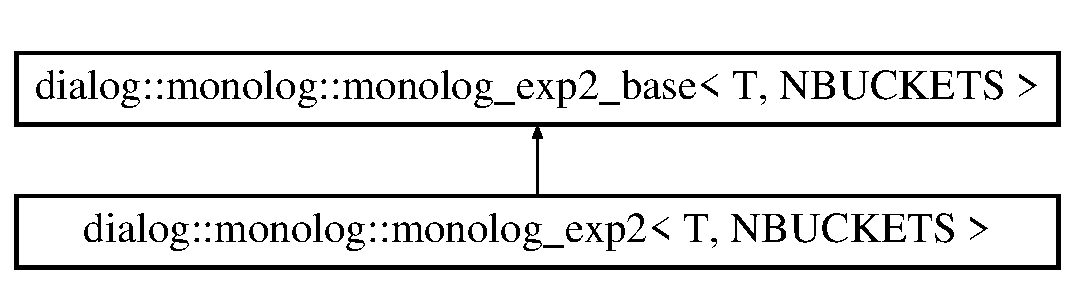
\includegraphics[height=2.000000cm]{classdialog_1_1monolog_1_1monolog__exp2}
\end{center}
\end{figure}
\subsection*{Public Types}
\begin{DoxyCompactItemize}
\item 
\mbox{\Hypertarget{classdialog_1_1monolog_1_1monolog__exp2_a34c79ea90c9e6e08e5ba2572b5373344}\label{classdialog_1_1monolog_1_1monolog__exp2_a34c79ea90c9e6e08e5ba2572b5373344}} 
typedef size\+\_\+t {\bfseries size\+\_\+type}
\item 
\mbox{\Hypertarget{classdialog_1_1monolog_1_1monolog__exp2_a48ff12ea0a19afa90c4ed768b2abe0d8}\label{classdialog_1_1monolog_1_1monolog__exp2_a48ff12ea0a19afa90c4ed768b2abe0d8}} 
typedef size\+\_\+t {\bfseries pos\+\_\+type}
\item 
\mbox{\Hypertarget{classdialog_1_1monolog_1_1monolog__exp2_aa56e194d4f9091f40c6799346fd82875}\label{classdialog_1_1monolog_1_1monolog__exp2_aa56e194d4f9091f40c6799346fd82875}} 
typedef T {\bfseries value\+\_\+type}
\item 
\mbox{\Hypertarget{classdialog_1_1monolog_1_1monolog__exp2_af5ab804b2a646c5e449e595c9fb2309b}\label{classdialog_1_1monolog_1_1monolog__exp2_af5ab804b2a646c5e449e595c9fb2309b}} 
typedef T {\bfseries difference\+\_\+type}
\item 
\mbox{\Hypertarget{classdialog_1_1monolog_1_1monolog__exp2_afb7ebe452ad7e4ce9fe56b021a1dc4a2}\label{classdialog_1_1monolog_1_1monolog__exp2_afb7ebe452ad7e4ce9fe56b021a1dc4a2}} 
typedef T $\ast$ {\bfseries pointer}
\item 
\mbox{\Hypertarget{classdialog_1_1monolog_1_1monolog__exp2_a5be0c26b9eba0deaf251ef535fcba405}\label{classdialog_1_1monolog_1_1monolog__exp2_a5be0c26b9eba0deaf251ef535fcba405}} 
typedef T {\bfseries reference}
\item 
\mbox{\Hypertarget{classdialog_1_1monolog_1_1monolog__exp2_a3dbe25f120cab3ba2754c327e7274b25}\label{classdialog_1_1monolog_1_1monolog__exp2_a3dbe25f120cab3ba2754c327e7274b25}} 
typedef \hyperlink{classdialog_1_1monolog_1_1monolog__iterator}{monolog\+\_\+iterator}$<$ \hyperlink{classdialog_1_1monolog_1_1monolog__exp2}{monolog\+\_\+exp2}$<$ T, N\+B\+U\+C\+K\+E\+TS $>$ $>$ {\bfseries iterator}
\item 
\mbox{\Hypertarget{classdialog_1_1monolog_1_1monolog__exp2_afb269a7cad947b4222037aff4bdf2158}\label{classdialog_1_1monolog_1_1monolog__exp2_afb269a7cad947b4222037aff4bdf2158}} 
typedef \hyperlink{classdialog_1_1monolog_1_1monolog__iterator}{monolog\+\_\+iterator}$<$ \hyperlink{classdialog_1_1monolog_1_1monolog__exp2}{monolog\+\_\+exp2}$<$ T, N\+B\+U\+C\+K\+E\+TS $>$ $>$ {\bfseries const\+\_\+iterator}
\end{DoxyCompactItemize}
\subsection*{Public Member Functions}
\begin{DoxyCompactItemize}
\item 
\mbox{\Hypertarget{classdialog_1_1monolog_1_1monolog__exp2_a751a37541284171868faebad27f89b31}\label{classdialog_1_1monolog_1_1monolog__exp2_a751a37541284171868faebad27f89b31}} 
size\+\_\+t {\bfseries reserve} (size\+\_\+t count)
\item 
\mbox{\Hypertarget{classdialog_1_1monolog_1_1monolog__exp2_a991b3996e814455616c2bbb045b25e25}\label{classdialog_1_1monolog_1_1monolog__exp2_a991b3996e814455616c2bbb045b25e25}} 
size\+\_\+t {\bfseries push\+\_\+back} (const T \&val)
\item 
\mbox{\Hypertarget{classdialog_1_1monolog_1_1monolog__exp2_a3ca865840be07349b8d9df1989ca5a46}\label{classdialog_1_1monolog_1_1monolog__exp2_a3ca865840be07349b8d9df1989ca5a46}} 
size\+\_\+t {\bfseries push\+\_\+back\+\_\+range} (const T \&start, const T \&end)
\item 
\mbox{\Hypertarget{classdialog_1_1monolog_1_1monolog__exp2_a53e9b057e39b26a9d91c56ad8a907b09}\label{classdialog_1_1monolog_1_1monolog__exp2_a53e9b057e39b26a9d91c56ad8a907b09}} 
const T \& {\bfseries at} (size\+\_\+t idx) const
\item 
\mbox{\Hypertarget{classdialog_1_1monolog_1_1monolog__exp2_a9564a4b217330641be63262c3f86843e}\label{classdialog_1_1monolog_1_1monolog__exp2_a9564a4b217330641be63262c3f86843e}} 
size\+\_\+t {\bfseries size} () const
\item 
\mbox{\Hypertarget{classdialog_1_1monolog_1_1monolog__exp2_a317fc0b23a841df31c0c4bfe0bbffdd7}\label{classdialog_1_1monolog_1_1monolog__exp2_a317fc0b23a841df31c0c4bfe0bbffdd7}} 
\hyperlink{classdialog_1_1monolog_1_1monolog__iterator}{iterator} {\bfseries begin} () const
\item 
\mbox{\Hypertarget{classdialog_1_1monolog_1_1monolog__exp2_a20e4165ab6a3cf979a18b65e2fa0999a}\label{classdialog_1_1monolog_1_1monolog__exp2_a20e4165ab6a3cf979a18b65e2fa0999a}} 
\hyperlink{classdialog_1_1monolog_1_1monolog__iterator}{iterator} {\bfseries end} () const
\end{DoxyCompactItemize}
\subsection*{Additional Inherited Members}


\subsection{Detailed Description}
\subsubsection*{template$<$class T, size\+\_\+t N\+B\+U\+C\+K\+E\+TS = 32$>$\newline
class dialog\+::monolog\+::monolog\+\_\+exp2$<$ T, N\+B\+U\+C\+K\+E\+T\+S $>$}

Relaxed (i.\+e., not linearizable) implementation for the Mono\+Log.

Maintains a single tail that ensures\+:
\begin{DoxyItemize}
\item Write operations are atomic 
\end{DoxyItemize}

The documentation for this class was generated from the following file\+:\begin{DoxyCompactItemize}
\item 
/\+Users/neil/\+Documents/\+Berkeley/research/dialog/libdialog/dialog/monolog\+\_\+exp2.\+h\end{DoxyCompactItemize}

\hypertarget{classdialog_1_1monolog_1_1monolog__exp2__base}{}\section{dialog\+:\+:monolog\+:\+:monolog\+\_\+exp2\+\_\+base$<$ T, N\+B\+U\+C\+K\+E\+TS $>$ Class Template Reference}
\label{classdialog_1_1monolog_1_1monolog__exp2__base}\index{dialog\+::monolog\+::monolog\+\_\+exp2\+\_\+base$<$ T, N\+B\+U\+C\+K\+E\+T\+S $>$@{dialog\+::monolog\+::monolog\+\_\+exp2\+\_\+base$<$ T, N\+B\+U\+C\+K\+E\+T\+S $>$}}
Inheritance diagram for dialog\+:\+:monolog\+:\+:monolog\+\_\+exp2\+\_\+base$<$ T, N\+B\+U\+C\+K\+E\+TS $>$\+:\begin{figure}[H]
\begin{center}
\leavevmode
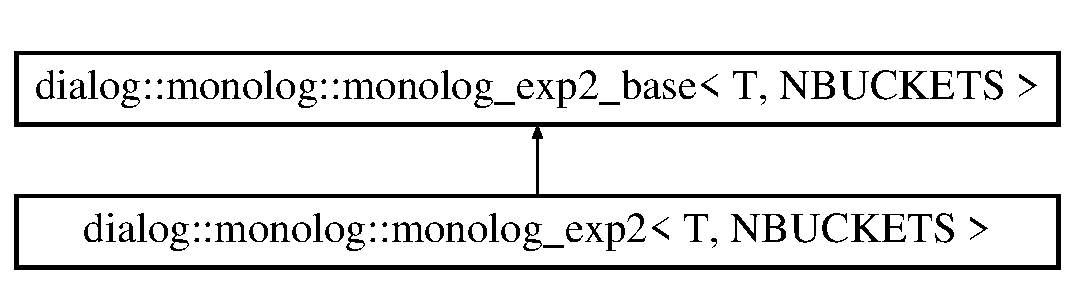
\includegraphics[height=2.000000cm]{classdialog_1_1monolog_1_1monolog__exp2__base}
\end{center}
\end{figure}
\subsection*{Public Types}
\begin{DoxyCompactItemize}
\item 
\mbox{\Hypertarget{classdialog_1_1monolog_1_1monolog__exp2__base_a58f02a832fcddb4ead166f769ad40a85}\label{classdialog_1_1monolog_1_1monolog__exp2__base_a58f02a832fcddb4ead166f769ad40a85}} 
typedef atomic\+::type$<$ T $\ast$ $>$ {\bfseries \+\_\+\+\_\+atomic\+\_\+bucket\+\_\+ref}
\end{DoxyCompactItemize}
\subsection*{Public Member Functions}
\begin{DoxyCompactItemize}
\item 
\hyperlink{classdialog_1_1monolog_1_1monolog__exp2__base_ac59fe74069159b44d64ed2395adb2fae}{monolog\+\_\+exp2\+\_\+base} ()
\item 
\hyperlink{classdialog_1_1monolog_1_1monolog__exp2__base_a4af0cf1b148d7b832d180da5c9ad389f}{$\sim$monolog\+\_\+exp2\+\_\+base} ()
\item 
void \hyperlink{classdialog_1_1monolog_1_1monolog__exp2__base_a86dd772a9b7beee2503a2349619a99ab}{ensure\+\_\+alloc} (size\+\_\+t start\+\_\+idx, size\+\_\+t end\+\_\+idx)
\item 
void \hyperlink{classdialog_1_1monolog_1_1monolog__exp2__base_a86d27f015adcd1320b4e1f811e1c1ceb}{set} (size\+\_\+t idx, const T val)
\item 
void \hyperlink{classdialog_1_1monolog_1_1monolog__exp2__base_ace9cdb67da6d6e9138705afb140b1560}{set\+\_\+unsafe} (size\+\_\+t idx, const T val)
\item 
void \hyperlink{classdialog_1_1monolog_1_1monolog__exp2__base_a11fb0491dea6bd8e0877a47c3f22708a}{set} (size\+\_\+t idx, const T $\ast$\hyperlink{structdialog_1_1data}{data}, size\+\_\+t len)
\item 
void \hyperlink{classdialog_1_1monolog_1_1monolog__exp2__base_a5e286b72175a394dfbb9bcf6e5c1fbc6}{set\+\_\+unsafe} (size\+\_\+t idx, const T $\ast$\hyperlink{structdialog_1_1data}{data}, size\+\_\+t len)
\item 
const T $\ast$ \hyperlink{classdialog_1_1monolog_1_1monolog__exp2__base_a76b101e66b927da18d6a723656a6a173}{ptr} (size\+\_\+t idx) const
\item 
const T \& \hyperlink{classdialog_1_1monolog_1_1monolog__exp2__base_acfb1656dd72bad1eba0d7e891899e3dc}{get} (size\+\_\+t idx) const
\item 
T \& \hyperlink{classdialog_1_1monolog_1_1monolog__exp2__base_acb8a92ddaabae330d33cb2bd9e14b642}{operator\mbox{[}$\,$\mbox{]}} (size\+\_\+t idx)
\item 
void \hyperlink{classdialog_1_1monolog_1_1monolog__exp2__base_abdff44f16e79714291fab191c9a9e19c}{get} (T $\ast$\hyperlink{structdialog_1_1data}{data}, size\+\_\+t idx, size\+\_\+t len) const
\item 
size\+\_\+t \hyperlink{classdialog_1_1monolog_1_1monolog__exp2__base_a908d3997fcc3790bced9e691223eb865}{storage\+\_\+size} () const
\end{DoxyCompactItemize}
\subsection*{Static Public Attributes}
\begin{DoxyCompactItemize}
\item 
\mbox{\Hypertarget{classdialog_1_1monolog_1_1monolog__exp2__base_af51f7c1502c45d94f2f85a173ddccce6}\label{classdialog_1_1monolog_1_1monolog__exp2__base_af51f7c1502c45d94f2f85a173ddccce6}} 
static const size\+\_\+t {\bfseries F\+BS} = 16
\item 
\mbox{\Hypertarget{classdialog_1_1monolog_1_1monolog__exp2__base_a8dc41c856d845d71fa96ce35a1918259}\label{classdialog_1_1monolog_1_1monolog__exp2__base_a8dc41c856d845d71fa96ce35a1918259}} 
static const size\+\_\+t {\bfseries F\+B\+S\+\_\+\+H\+I\+B\+IT} = 4
\end{DoxyCompactItemize}
\subsection*{Protected Member Functions}
\begin{DoxyCompactItemize}
\item 
\mbox{\Hypertarget{classdialog_1_1monolog_1_1monolog__exp2__base_a2566df9503c1dae556d2430535a8fa26}\label{classdialog_1_1monolog_1_1monolog__exp2__base_a2566df9503c1dae556d2430535a8fa26}} 
T $\ast$ {\bfseries try\+\_\+allocate\+\_\+bucket} (size\+\_\+t bucket\+\_\+idx)
\end{DoxyCompactItemize}
\subsection*{Protected Attributes}
\begin{DoxyCompactItemize}
\item 
\mbox{\Hypertarget{classdialog_1_1monolog_1_1monolog__exp2__base_a2abe7a8d0a1da433ba79fe4e340c461f}\label{classdialog_1_1monolog_1_1monolog__exp2__base_a2abe7a8d0a1da433ba79fe4e340c461f}} 
std\+::array$<$ \+\_\+\+\_\+atomic\+\_\+bucket\+\_\+ref, N\+B\+U\+C\+K\+E\+TS $>$ {\bfseries buckets\+\_\+}
\end{DoxyCompactItemize}


\subsection{Constructor \& Destructor Documentation}
\mbox{\Hypertarget{classdialog_1_1monolog_1_1monolog__exp2__base_ac59fe74069159b44d64ed2395adb2fae}\label{classdialog_1_1monolog_1_1monolog__exp2__base_ac59fe74069159b44d64ed2395adb2fae}} 
\index{dialog\+::monolog\+::monolog\+\_\+exp2\+\_\+base@{dialog\+::monolog\+::monolog\+\_\+exp2\+\_\+base}!monolog\+\_\+exp2\+\_\+base@{monolog\+\_\+exp2\+\_\+base}}
\index{monolog\+\_\+exp2\+\_\+base@{monolog\+\_\+exp2\+\_\+base}!dialog\+::monolog\+::monolog\+\_\+exp2\+\_\+base@{dialog\+::monolog\+::monolog\+\_\+exp2\+\_\+base}}
\subsubsection{\texorpdfstring{monolog\+\_\+exp2\+\_\+base()}{monolog\_exp2\_base()}}
{\footnotesize\ttfamily template$<$class T , size\+\_\+t N\+B\+U\+C\+K\+E\+TS = 32$>$ \\
\hyperlink{classdialog_1_1monolog_1_1monolog__exp2__base}{dialog\+::monolog\+::monolog\+\_\+exp2\+\_\+base}$<$ T, N\+B\+U\+C\+K\+E\+TS $>$\+::\hyperlink{classdialog_1_1monolog_1_1monolog__exp2__base}{monolog\+\_\+exp2\+\_\+base} (\begin{DoxyParamCaption}{ }\end{DoxyParamCaption})\hspace{0.3cm}{\ttfamily [inline]}}

The default constructor that initializes all of the buckets for the monolog \mbox{\Hypertarget{classdialog_1_1monolog_1_1monolog__exp2__base_a4af0cf1b148d7b832d180da5c9ad389f}\label{classdialog_1_1monolog_1_1monolog__exp2__base_a4af0cf1b148d7b832d180da5c9ad389f}} 
\index{dialog\+::monolog\+::monolog\+\_\+exp2\+\_\+base@{dialog\+::monolog\+::monolog\+\_\+exp2\+\_\+base}!````~monolog\+\_\+exp2\+\_\+base@{$\sim$monolog\+\_\+exp2\+\_\+base}}
\index{````~monolog\+\_\+exp2\+\_\+base@{$\sim$monolog\+\_\+exp2\+\_\+base}!dialog\+::monolog\+::monolog\+\_\+exp2\+\_\+base@{dialog\+::monolog\+::monolog\+\_\+exp2\+\_\+base}}
\subsubsection{\texorpdfstring{$\sim$monolog\+\_\+exp2\+\_\+base()}{~monolog\_exp2\_base()}}
{\footnotesize\ttfamily template$<$class T , size\+\_\+t N\+B\+U\+C\+K\+E\+TS = 32$>$ \\
\hyperlink{classdialog_1_1monolog_1_1monolog__exp2__base}{dialog\+::monolog\+::monolog\+\_\+exp2\+\_\+base}$<$ T, N\+B\+U\+C\+K\+E\+TS $>$\+::$\sim$\hyperlink{classdialog_1_1monolog_1_1monolog__exp2__base}{monolog\+\_\+exp2\+\_\+base} (\begin{DoxyParamCaption}{ }\end{DoxyParamCaption})\hspace{0.3cm}{\ttfamily [inline]}}

The default destructor that deletes all of the buckets 

\subsection{Member Function Documentation}
\mbox{\Hypertarget{classdialog_1_1monolog_1_1monolog__exp2__base_a86dd772a9b7beee2503a2349619a99ab}\label{classdialog_1_1monolog_1_1monolog__exp2__base_a86dd772a9b7beee2503a2349619a99ab}} 
\index{dialog\+::monolog\+::monolog\+\_\+exp2\+\_\+base@{dialog\+::monolog\+::monolog\+\_\+exp2\+\_\+base}!ensure\+\_\+alloc@{ensure\+\_\+alloc}}
\index{ensure\+\_\+alloc@{ensure\+\_\+alloc}!dialog\+::monolog\+::monolog\+\_\+exp2\+\_\+base@{dialog\+::monolog\+::monolog\+\_\+exp2\+\_\+base}}
\subsubsection{\texorpdfstring{ensure\+\_\+alloc()}{ensure\_alloc()}}
{\footnotesize\ttfamily template$<$class T , size\+\_\+t N\+B\+U\+C\+K\+E\+TS = 32$>$ \\
void \hyperlink{classdialog_1_1monolog_1_1monolog__exp2__base}{dialog\+::monolog\+::monolog\+\_\+exp2\+\_\+base}$<$ T, N\+B\+U\+C\+K\+E\+TS $>$\+::ensure\+\_\+alloc (\begin{DoxyParamCaption}\item[{size\+\_\+t}]{start\+\_\+idx,  }\item[{size\+\_\+t}]{end\+\_\+idx }\end{DoxyParamCaption})\hspace{0.3cm}{\ttfamily [inline]}}

Allocates space for buckets between the indices 
\begin{DoxyParams}{Parameters}
{\em start\+\_\+idx} & The start index \\
\hline
{\em end\+\_\+idx} & The end index \\
\hline
\end{DoxyParams}
\mbox{\Hypertarget{classdialog_1_1monolog_1_1monolog__exp2__base_acfb1656dd72bad1eba0d7e891899e3dc}\label{classdialog_1_1monolog_1_1monolog__exp2__base_acfb1656dd72bad1eba0d7e891899e3dc}} 
\index{dialog\+::monolog\+::monolog\+\_\+exp2\+\_\+base@{dialog\+::monolog\+::monolog\+\_\+exp2\+\_\+base}!get@{get}}
\index{get@{get}!dialog\+::monolog\+::monolog\+\_\+exp2\+\_\+base@{dialog\+::monolog\+::monolog\+\_\+exp2\+\_\+base}}
\subsubsection{\texorpdfstring{get()}{get()}\hspace{0.1cm}{\footnotesize\ttfamily [1/2]}}
{\footnotesize\ttfamily template$<$class T , size\+\_\+t N\+B\+U\+C\+K\+E\+TS = 32$>$ \\
const T\& \hyperlink{classdialog_1_1monolog_1_1monolog__exp2__base}{dialog\+::monolog\+::monolog\+\_\+exp2\+\_\+base}$<$ T, N\+B\+U\+C\+K\+E\+TS $>$\+::get (\begin{DoxyParamCaption}\item[{size\+\_\+t}]{idx }\end{DoxyParamCaption}) const\hspace{0.3cm}{\ttfamily [inline]}}

Gets the data at index idx. 
\begin{DoxyParams}{Parameters}
{\em idx} & The index of where to get the data \\
\hline
\end{DoxyParams}
\begin{DoxyReturn}{Returns}
A reference to the data at that index 
\end{DoxyReturn}
\mbox{\Hypertarget{classdialog_1_1monolog_1_1monolog__exp2__base_abdff44f16e79714291fab191c9a9e19c}\label{classdialog_1_1monolog_1_1monolog__exp2__base_abdff44f16e79714291fab191c9a9e19c}} 
\index{dialog\+::monolog\+::monolog\+\_\+exp2\+\_\+base@{dialog\+::monolog\+::monolog\+\_\+exp2\+\_\+base}!get@{get}}
\index{get@{get}!dialog\+::monolog\+::monolog\+\_\+exp2\+\_\+base@{dialog\+::monolog\+::monolog\+\_\+exp2\+\_\+base}}
\subsubsection{\texorpdfstring{get()}{get()}\hspace{0.1cm}{\footnotesize\ttfamily [2/2]}}
{\footnotesize\ttfamily template$<$class T , size\+\_\+t N\+B\+U\+C\+K\+E\+TS = 32$>$ \\
void \hyperlink{classdialog_1_1monolog_1_1monolog__exp2__base}{dialog\+::monolog\+::monolog\+\_\+exp2\+\_\+base}$<$ T, N\+B\+U\+C\+K\+E\+TS $>$\+::get (\begin{DoxyParamCaption}\item[{T $\ast$}]{data,  }\item[{size\+\_\+t}]{idx,  }\item[{size\+\_\+t}]{len }\end{DoxyParamCaption}) const\hspace{0.3cm}{\ttfamily [inline]}}

Copies a contiguous region of the Mono\+Log base into the provided buffer.\+The buffer should have sufficient space to hold the data requested, otherwise undefined behavior may result. 
\begin{DoxyParams}{Parameters}
{\em data} & The data to be copied \\
\hline
{\em idx} & The index for where the data is copied to \\
\hline
{\em len} & The length of the buffer \\
\hline
\end{DoxyParams}
\mbox{\Hypertarget{classdialog_1_1monolog_1_1monolog__exp2__base_acb8a92ddaabae330d33cb2bd9e14b642}\label{classdialog_1_1monolog_1_1monolog__exp2__base_acb8a92ddaabae330d33cb2bd9e14b642}} 
\index{dialog\+::monolog\+::monolog\+\_\+exp2\+\_\+base@{dialog\+::monolog\+::monolog\+\_\+exp2\+\_\+base}!operator\mbox{[}\mbox{]}@{operator[]}}
\index{operator\mbox{[}\mbox{]}@{operator[]}!dialog\+::monolog\+::monolog\+\_\+exp2\+\_\+base@{dialog\+::monolog\+::monolog\+\_\+exp2\+\_\+base}}
\subsubsection{\texorpdfstring{operator[]()}{operator[]()}}
{\footnotesize\ttfamily template$<$class T , size\+\_\+t N\+B\+U\+C\+K\+E\+TS = 32$>$ \\
T\& \hyperlink{classdialog_1_1monolog_1_1monolog__exp2__base}{dialog\+::monolog\+::monolog\+\_\+exp2\+\_\+base}$<$ T, N\+B\+U\+C\+K\+E\+TS $>$\+::operator\mbox{[}$\,$\mbox{]} (\begin{DoxyParamCaption}\item[{size\+\_\+t}]{idx }\end{DoxyParamCaption})\hspace{0.3cm}{\ttfamily [inline]}}

Accesses the data at a specific index 
\begin{DoxyParams}{Parameters}
{\em idx} & The index of what data to get \\
\hline
\end{DoxyParams}
\begin{DoxyReturn}{Returns}
A reference to the data at the index 
\end{DoxyReturn}
\mbox{\Hypertarget{classdialog_1_1monolog_1_1monolog__exp2__base_a76b101e66b927da18d6a723656a6a173}\label{classdialog_1_1monolog_1_1monolog__exp2__base_a76b101e66b927da18d6a723656a6a173}} 
\index{dialog\+::monolog\+::monolog\+\_\+exp2\+\_\+base@{dialog\+::monolog\+::monolog\+\_\+exp2\+\_\+base}!ptr@{ptr}}
\index{ptr@{ptr}!dialog\+::monolog\+::monolog\+\_\+exp2\+\_\+base@{dialog\+::monolog\+::monolog\+\_\+exp2\+\_\+base}}
\subsubsection{\texorpdfstring{ptr()}{ptr()}}
{\footnotesize\ttfamily template$<$class T , size\+\_\+t N\+B\+U\+C\+K\+E\+TS = 32$>$ \\
const T$\ast$ \hyperlink{classdialog_1_1monolog_1_1monolog__exp2__base}{dialog\+::monolog\+::monolog\+\_\+exp2\+\_\+base}$<$ T, N\+B\+U\+C\+K\+E\+TS $>$\+::ptr (\begin{DoxyParamCaption}\item[{size\+\_\+t}]{idx }\end{DoxyParamCaption}) const\hspace{0.3cm}{\ttfamily [inline]}}

Gets the pointer to the data specified by the index 
\begin{DoxyParams}{Parameters}
{\em idx} & The index of where to get the data \\
\hline
\end{DoxyParams}
\begin{DoxyReturn}{Returns}
The pointer to the region 
\end{DoxyReturn}
\mbox{\Hypertarget{classdialog_1_1monolog_1_1monolog__exp2__base_a86d27f015adcd1320b4e1f811e1c1ceb}\label{classdialog_1_1monolog_1_1monolog__exp2__base_a86d27f015adcd1320b4e1f811e1c1ceb}} 
\index{dialog\+::monolog\+::monolog\+\_\+exp2\+\_\+base@{dialog\+::monolog\+::monolog\+\_\+exp2\+\_\+base}!set@{set}}
\index{set@{set}!dialog\+::monolog\+::monolog\+\_\+exp2\+\_\+base@{dialog\+::monolog\+::monolog\+\_\+exp2\+\_\+base}}
\subsubsection{\texorpdfstring{set()}{set()}\hspace{0.1cm}{\footnotesize\ttfamily [1/2]}}
{\footnotesize\ttfamily template$<$class T , size\+\_\+t N\+B\+U\+C\+K\+E\+TS = 32$>$ \\
void \hyperlink{classdialog_1_1monolog_1_1monolog__exp2__base}{dialog\+::monolog\+::monolog\+\_\+exp2\+\_\+base}$<$ T, N\+B\+U\+C\+K\+E\+TS $>$\+::set (\begin{DoxyParamCaption}\item[{size\+\_\+t}]{idx,  }\item[{const T}]{val }\end{DoxyParamCaption})\hspace{0.3cm}{\ttfamily [inline]}}

Sets the data at index idx to val. Allocates memory if necessary. 
\begin{DoxyParams}{Parameters}
{\em idx} & The specified index \\
\hline
{\em val} & The data to be set at the index \\
\hline
\end{DoxyParams}
\mbox{\Hypertarget{classdialog_1_1monolog_1_1monolog__exp2__base_a11fb0491dea6bd8e0877a47c3f22708a}\label{classdialog_1_1monolog_1_1monolog__exp2__base_a11fb0491dea6bd8e0877a47c3f22708a}} 
\index{dialog\+::monolog\+::monolog\+\_\+exp2\+\_\+base@{dialog\+::monolog\+::monolog\+\_\+exp2\+\_\+base}!set@{set}}
\index{set@{set}!dialog\+::monolog\+::monolog\+\_\+exp2\+\_\+base@{dialog\+::monolog\+::monolog\+\_\+exp2\+\_\+base}}
\subsubsection{\texorpdfstring{set()}{set()}\hspace{0.1cm}{\footnotesize\ttfamily [2/2]}}
{\footnotesize\ttfamily template$<$class T , size\+\_\+t N\+B\+U\+C\+K\+E\+TS = 32$>$ \\
void \hyperlink{classdialog_1_1monolog_1_1monolog__exp2__base}{dialog\+::monolog\+::monolog\+\_\+exp2\+\_\+base}$<$ T, N\+B\+U\+C\+K\+E\+TS $>$\+::set (\begin{DoxyParamCaption}\item[{size\+\_\+t}]{idx,  }\item[{const T $\ast$}]{data,  }\item[{size\+\_\+t}]{len }\end{DoxyParamCaption})\hspace{0.3cm}{\ttfamily [inline]}}

Sets a contiguous region of the Mono\+Log base to the provided data. 
\begin{DoxyParams}{Parameters}
{\em idx} & The specified index \\
\hline
{\em data} & The data that needs to be stored \\
\hline
{\em len} & The length of the region \\
\hline
\end{DoxyParams}
\mbox{\Hypertarget{classdialog_1_1monolog_1_1monolog__exp2__base_ace9cdb67da6d6e9138705afb140b1560}\label{classdialog_1_1monolog_1_1monolog__exp2__base_ace9cdb67da6d6e9138705afb140b1560}} 
\index{dialog\+::monolog\+::monolog\+\_\+exp2\+\_\+base@{dialog\+::monolog\+::monolog\+\_\+exp2\+\_\+base}!set\+\_\+unsafe@{set\+\_\+unsafe}}
\index{set\+\_\+unsafe@{set\+\_\+unsafe}!dialog\+::monolog\+::monolog\+\_\+exp2\+\_\+base@{dialog\+::monolog\+::monolog\+\_\+exp2\+\_\+base}}
\subsubsection{\texorpdfstring{set\+\_\+unsafe()}{set\_unsafe()}\hspace{0.1cm}{\footnotesize\ttfamily [1/2]}}
{\footnotesize\ttfamily template$<$class T , size\+\_\+t N\+B\+U\+C\+K\+E\+TS = 32$>$ \\
void \hyperlink{classdialog_1_1monolog_1_1monolog__exp2__base}{dialog\+::monolog\+::monolog\+\_\+exp2\+\_\+base}$<$ T, N\+B\+U\+C\+K\+E\+TS $>$\+::set\+\_\+unsafe (\begin{DoxyParamCaption}\item[{size\+\_\+t}]{idx,  }\item[{const T}]{val }\end{DoxyParamCaption})\hspace{0.3cm}{\ttfamily [inline]}}

Sets the data at index idx to val. Does N\+OT allocate memory -- ensure memory is allocated before calling this function. 
\begin{DoxyParams}{Parameters}
{\em idx} & The specified index \\
\hline
{\em val} & The data to be set at the index \\
\hline
\end{DoxyParams}
\mbox{\Hypertarget{classdialog_1_1monolog_1_1monolog__exp2__base_a5e286b72175a394dfbb9bcf6e5c1fbc6}\label{classdialog_1_1monolog_1_1monolog__exp2__base_a5e286b72175a394dfbb9bcf6e5c1fbc6}} 
\index{dialog\+::monolog\+::monolog\+\_\+exp2\+\_\+base@{dialog\+::monolog\+::monolog\+\_\+exp2\+\_\+base}!set\+\_\+unsafe@{set\+\_\+unsafe}}
\index{set\+\_\+unsafe@{set\+\_\+unsafe}!dialog\+::monolog\+::monolog\+\_\+exp2\+\_\+base@{dialog\+::monolog\+::monolog\+\_\+exp2\+\_\+base}}
\subsubsection{\texorpdfstring{set\+\_\+unsafe()}{set\_unsafe()}\hspace{0.1cm}{\footnotesize\ttfamily [2/2]}}
{\footnotesize\ttfamily template$<$class T , size\+\_\+t N\+B\+U\+C\+K\+E\+TS = 32$>$ \\
void \hyperlink{classdialog_1_1monolog_1_1monolog__exp2__base}{dialog\+::monolog\+::monolog\+\_\+exp2\+\_\+base}$<$ T, N\+B\+U\+C\+K\+E\+TS $>$\+::set\+\_\+unsafe (\begin{DoxyParamCaption}\item[{size\+\_\+t}]{idx,  }\item[{const T $\ast$}]{data,  }\item[{size\+\_\+t}]{len }\end{DoxyParamCaption})\hspace{0.3cm}{\ttfamily [inline]}}

Sets a contiguous region of the Mono\+Log base to the provided data. Does N\+OT allocate memory -- ensure memory is allocated before calling this function.


\begin{DoxyParams}{Parameters}
{\em idx} & The specified index \\
\hline
{\em data} & The data to be stored \\
\hline
{\em len} & The length of the region \\
\hline
\end{DoxyParams}
\mbox{\Hypertarget{classdialog_1_1monolog_1_1monolog__exp2__base_a908d3997fcc3790bced9e691223eb865}\label{classdialog_1_1monolog_1_1monolog__exp2__base_a908d3997fcc3790bced9e691223eb865}} 
\index{dialog\+::monolog\+::monolog\+\_\+exp2\+\_\+base@{dialog\+::monolog\+::monolog\+\_\+exp2\+\_\+base}!storage\+\_\+size@{storage\+\_\+size}}
\index{storage\+\_\+size@{storage\+\_\+size}!dialog\+::monolog\+::monolog\+\_\+exp2\+\_\+base@{dialog\+::monolog\+::monolog\+\_\+exp2\+\_\+base}}
\subsubsection{\texorpdfstring{storage\+\_\+size()}{storage\_size()}}
{\footnotesize\ttfamily template$<$class T , size\+\_\+t N\+B\+U\+C\+K\+E\+TS = 32$>$ \\
size\+\_\+t \hyperlink{classdialog_1_1monolog_1_1monolog__exp2__base}{dialog\+::monolog\+::monolog\+\_\+exp2\+\_\+base}$<$ T, N\+B\+U\+C\+K\+E\+TS $>$\+::storage\+\_\+size (\begin{DoxyParamCaption}{ }\end{DoxyParamCaption}) const\hspace{0.3cm}{\ttfamily [inline]}}

Gets the size of the storage space \begin{DoxyReturn}{Returns}
The size of storage in bytes 
\end{DoxyReturn}


The documentation for this class was generated from the following file\+:\begin{DoxyCompactItemize}
\item 
/\+Users/neil/\+Documents/\+Berkeley/research/dialog/libdialog/dialog/monolog\+\_\+exp2.\+h\end{DoxyCompactItemize}

\hypertarget{classdialog_1_1monolog_1_1monolog__exp2__linear}{}\section{dialog\+:\+:monolog\+:\+:monolog\+\_\+exp2\+\_\+linear$<$ T, N\+C\+O\+N\+T\+A\+I\+N\+E\+RS, B\+U\+C\+K\+E\+T\+\_\+\+S\+I\+ZE $>$ Class Template Reference}
\label{classdialog_1_1monolog_1_1monolog__exp2__linear}\index{dialog\+::monolog\+::monolog\+\_\+exp2\+\_\+linear$<$ T, N\+C\+O\+N\+T\+A\+I\+N\+E\+R\+S, B\+U\+C\+K\+E\+T\+\_\+\+S\+I\+Z\+E $>$@{dialog\+::monolog\+::monolog\+\_\+exp2\+\_\+linear$<$ T, N\+C\+O\+N\+T\+A\+I\+N\+E\+R\+S, B\+U\+C\+K\+E\+T\+\_\+\+S\+I\+Z\+E $>$}}


{\ttfamily \#include $<$monolog\+\_\+exp2\+\_\+linear.\+h$>$}

Inheritance diagram for dialog\+:\+:monolog\+:\+:monolog\+\_\+exp2\+\_\+linear$<$ T, N\+C\+O\+N\+T\+A\+I\+N\+E\+RS, B\+U\+C\+K\+E\+T\+\_\+\+S\+I\+ZE $>$\+:\begin{figure}[H]
\begin{center}
\leavevmode
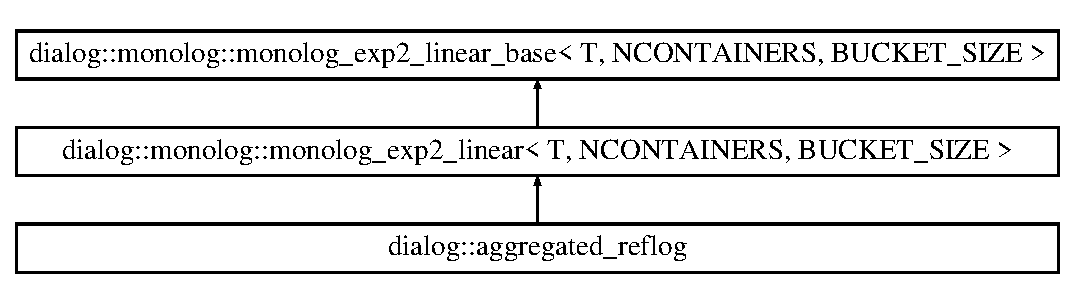
\includegraphics[height=3.000000cm]{classdialog_1_1monolog_1_1monolog__exp2__linear}
\end{center}
\end{figure}
\subsection*{Public Types}
\begin{DoxyCompactItemize}
\item 
\mbox{\Hypertarget{classdialog_1_1monolog_1_1monolog__exp2__linear_a15166cf5aeea7f93b9a792bf414ce115}\label{classdialog_1_1monolog_1_1monolog__exp2__linear_a15166cf5aeea7f93b9a792bf414ce115}} 
typedef size\+\_\+t {\bfseries size\+\_\+type}
\item 
\mbox{\Hypertarget{classdialog_1_1monolog_1_1monolog__exp2__linear_afed86e0a1005af29c645daa8d0b4479c}\label{classdialog_1_1monolog_1_1monolog__exp2__linear_afed86e0a1005af29c645daa8d0b4479c}} 
typedef size\+\_\+t {\bfseries pos\+\_\+type}
\item 
\mbox{\Hypertarget{classdialog_1_1monolog_1_1monolog__exp2__linear_a93b4f0d3a06947fff0b4a70aef0d7f2d}\label{classdialog_1_1monolog_1_1monolog__exp2__linear_a93b4f0d3a06947fff0b4a70aef0d7f2d}} 
typedef T {\bfseries value\+\_\+type}
\item 
\mbox{\Hypertarget{classdialog_1_1monolog_1_1monolog__exp2__linear_acbe4c0d63df24a78bd42af4f898355fe}\label{classdialog_1_1monolog_1_1monolog__exp2__linear_acbe4c0d63df24a78bd42af4f898355fe}} 
typedef T {\bfseries difference\+\_\+type}
\item 
\mbox{\Hypertarget{classdialog_1_1monolog_1_1monolog__exp2__linear_aa7d8ccbac0565677b10cbe2cdab2d4ae}\label{classdialog_1_1monolog_1_1monolog__exp2__linear_aa7d8ccbac0565677b10cbe2cdab2d4ae}} 
typedef T $\ast$ {\bfseries pointer}
\item 
\mbox{\Hypertarget{classdialog_1_1monolog_1_1monolog__exp2__linear_a02bfeebfe3a8ae69fe657396abeccc66}\label{classdialog_1_1monolog_1_1monolog__exp2__linear_a02bfeebfe3a8ae69fe657396abeccc66}} 
typedef T {\bfseries reference}
\item 
\mbox{\Hypertarget{classdialog_1_1monolog_1_1monolog__exp2__linear_a6cc9ff2c6f3d75efaa59cdfc6acc1dab}\label{classdialog_1_1monolog_1_1monolog__exp2__linear_a6cc9ff2c6f3d75efaa59cdfc6acc1dab}} 
typedef \hyperlink{classdialog_1_1monolog_1_1monolog__iterator}{monolog\+\_\+iterator}$<$ \hyperlink{classdialog_1_1monolog_1_1monolog__exp2__linear}{monolog\+\_\+exp2\+\_\+linear}$<$ T, N\+C\+O\+N\+T\+A\+I\+N\+E\+RS $>$ $>$ {\bfseries iterator}
\item 
\mbox{\Hypertarget{classdialog_1_1monolog_1_1monolog__exp2__linear_a2e472bb54dec91ebb9eb602a40404aed}\label{classdialog_1_1monolog_1_1monolog__exp2__linear_a2e472bb54dec91ebb9eb602a40404aed}} 
typedef \hyperlink{classdialog_1_1monolog_1_1monolog__iterator}{monolog\+\_\+iterator}$<$ \hyperlink{classdialog_1_1monolog_1_1monolog__exp2__linear}{monolog\+\_\+exp2\+\_\+linear}$<$ T, N\+C\+O\+N\+T\+A\+I\+N\+E\+RS $>$ $>$ {\bfseries const\+\_\+iterator}
\end{DoxyCompactItemize}
\subsection*{Public Member Functions}
\begin{DoxyCompactItemize}
\item 
\mbox{\Hypertarget{classdialog_1_1monolog_1_1monolog__exp2__linear_a460ce1e9eb9b3211965b71234e32b6b6}\label{classdialog_1_1monolog_1_1monolog__exp2__linear_a460ce1e9eb9b3211965b71234e32b6b6}} 
size\+\_\+t {\bfseries reserve} (size\+\_\+t count)
\item 
\mbox{\Hypertarget{classdialog_1_1monolog_1_1monolog__exp2__linear_ae9a341fbf7643bc21da4b4cefc73fd85}\label{classdialog_1_1monolog_1_1monolog__exp2__linear_ae9a341fbf7643bc21da4b4cefc73fd85}} 
size\+\_\+t {\bfseries push\+\_\+back} (const T \&val)
\item 
\mbox{\Hypertarget{classdialog_1_1monolog_1_1monolog__exp2__linear_a48919dd298c662a0568a3661a4ab6f43}\label{classdialog_1_1monolog_1_1monolog__exp2__linear_a48919dd298c662a0568a3661a4ab6f43}} 
size\+\_\+t {\bfseries push\+\_\+back\+\_\+range} (const T \&start, const T \&end)
\item 
\mbox{\Hypertarget{classdialog_1_1monolog_1_1monolog__exp2__linear_ac947d45a45c5b53f579d11607e9e1983}\label{classdialog_1_1monolog_1_1monolog__exp2__linear_ac947d45a45c5b53f579d11607e9e1983}} 
const T \& {\bfseries at} (size\+\_\+t idx) const
\item 
\mbox{\Hypertarget{classdialog_1_1monolog_1_1monolog__exp2__linear_a79afc1146fd5f4103f7f2e7c5335c46c}\label{classdialog_1_1monolog_1_1monolog__exp2__linear_a79afc1146fd5f4103f7f2e7c5335c46c}} 
size\+\_\+t {\bfseries size} () const
\item 
\mbox{\Hypertarget{classdialog_1_1monolog_1_1monolog__exp2__linear_a6a78122f3c49c057f9cd4087ec781489}\label{classdialog_1_1monolog_1_1monolog__exp2__linear_a6a78122f3c49c057f9cd4087ec781489}} 
\hyperlink{classdialog_1_1monolog_1_1monolog__iterator}{iterator} {\bfseries begin} () const
\item 
\mbox{\Hypertarget{classdialog_1_1monolog_1_1monolog__exp2__linear_a1231b24008d59334d0fb609690a55bb2}\label{classdialog_1_1monolog_1_1monolog__exp2__linear_a1231b24008d59334d0fb609690a55bb2}} 
\hyperlink{classdialog_1_1monolog_1_1monolog__iterator}{iterator} {\bfseries end} () const
\end{DoxyCompactItemize}
\subsection*{Additional Inherited Members}


\subsection{Detailed Description}
\subsubsection*{template$<$class T, size\+\_\+t N\+C\+O\+N\+T\+A\+I\+N\+E\+RS = 32, size\+\_\+t B\+U\+C\+K\+E\+T\+\_\+\+S\+I\+ZE = 1024$>$\newline
class dialog\+::monolog\+::monolog\+\_\+exp2\+\_\+linear$<$ T, N\+C\+O\+N\+T\+A\+I\+N\+E\+R\+S, B\+U\+C\+K\+E\+T\+\_\+\+S\+I\+Z\+E $>$}

Relaxed (i.\+e., not linearizable) implementation for the Mono\+Log.

Maintains a single tail that ensures\+:
\begin{DoxyItemize}
\item Write operations are atomic 
\end{DoxyItemize}

The documentation for this class was generated from the following file\+:\begin{DoxyCompactItemize}
\item 
/\+Users/neil/\+Documents/\+Berkeley/research/dialog/libdialog/dialog/monolog\+\_\+exp2\+\_\+linear.\+h\end{DoxyCompactItemize}

\hypertarget{classdialog_1_1monolog_1_1monolog__exp2__linear__base}{}\section{dialog\+:\+:monolog\+:\+:monolog\+\_\+exp2\+\_\+linear\+\_\+base$<$ T, N\+C\+O\+N\+T\+A\+I\+N\+E\+RS, B\+U\+C\+K\+E\+T\+\_\+\+S\+I\+ZE $>$ Class Template Reference}
\label{classdialog_1_1monolog_1_1monolog__exp2__linear__base}\index{dialog\+::monolog\+::monolog\+\_\+exp2\+\_\+linear\+\_\+base$<$ T, N\+C\+O\+N\+T\+A\+I\+N\+E\+R\+S, B\+U\+C\+K\+E\+T\+\_\+\+S\+I\+Z\+E $>$@{dialog\+::monolog\+::monolog\+\_\+exp2\+\_\+linear\+\_\+base$<$ T, N\+C\+O\+N\+T\+A\+I\+N\+E\+R\+S, B\+U\+C\+K\+E\+T\+\_\+\+S\+I\+Z\+E $>$}}


{\ttfamily \#include $<$monolog\+\_\+exp2\+\_\+linear.\+h$>$}

Inheritance diagram for dialog\+:\+:monolog\+:\+:monolog\+\_\+exp2\+\_\+linear\+\_\+base$<$ T, N\+C\+O\+N\+T\+A\+I\+N\+E\+RS, B\+U\+C\+K\+E\+T\+\_\+\+S\+I\+ZE $>$\+:\begin{figure}[H]
\begin{center}
\leavevmode
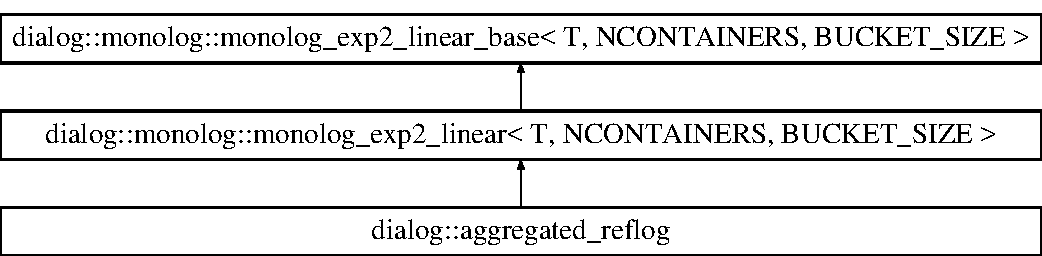
\includegraphics[height=3.000000cm]{classdialog_1_1monolog_1_1monolog__exp2__linear__base}
\end{center}
\end{figure}
\subsection*{Public Types}
\begin{DoxyCompactItemize}
\item 
\mbox{\Hypertarget{classdialog_1_1monolog_1_1monolog__exp2__linear__base_a903e99e4a8ae7f24bff57366a5f110b2}\label{classdialog_1_1monolog_1_1monolog__exp2__linear__base_a903e99e4a8ae7f24bff57366a5f110b2}} 
typedef atomic\+::type$<$ T $\ast$ $>$ {\bfseries \+\_\+\+\_\+atomic\+\_\+bucket\+\_\+ref}
\item 
\mbox{\Hypertarget{classdialog_1_1monolog_1_1monolog__exp2__linear__base_ae0189ef8c9f918cec38c878f5399c358}\label{classdialog_1_1monolog_1_1monolog__exp2__linear__base_ae0189ef8c9f918cec38c878f5399c358}} 
typedef atomic\+::type$<$ \+\_\+\+\_\+atomic\+\_\+bucket\+\_\+ref $\ast$ $>$ {\bfseries \+\_\+\+\_\+atomic\+\_\+bucket\+\_\+container\+\_\+ref}
\end{DoxyCompactItemize}
\subsection*{Public Member Functions}
\begin{DoxyCompactItemize}
\item 
void \hyperlink{classdialog_1_1monolog_1_1monolog__exp2__linear__base_a6daa5a4785866597eecfcdae2e333d0e}{ensure\+\_\+alloc} (size\+\_\+t start\+\_\+idx, size\+\_\+t end\+\_\+idx)
\item 
void \hyperlink{classdialog_1_1monolog_1_1monolog__exp2__linear__base_af292efeb7faae83c3f9e24f77a7f1fd8}{set} (size\+\_\+t idx, const T val)
\item 
void \hyperlink{classdialog_1_1monolog_1_1monolog__exp2__linear__base_a7adee243bf98901dbeb49c600ead38a5}{set\+\_\+unsafe} (size\+\_\+t idx, const T val)
\item 
void \hyperlink{classdialog_1_1monolog_1_1monolog__exp2__linear__base_a17d6ac9dfede2addd128f99cc7ea72bb}{set} (size\+\_\+t idx, const T $\ast$\hyperlink{structdialog_1_1data}{data}, size\+\_\+t len)
\item 
void \hyperlink{classdialog_1_1monolog_1_1monolog__exp2__linear__base_af4641b004a2e4341411872e5cfa9970d}{set\+\_\+unsafe} (size\+\_\+t idx, const T $\ast$\hyperlink{structdialog_1_1data}{data}, size\+\_\+t len)
\item 
const T $\ast$ \hyperlink{classdialog_1_1monolog_1_1monolog__exp2__linear__base_a73c30e25123e9b74ee03905a82a91c07}{ptr} (size\+\_\+t idx) const
\item 
const T \& \hyperlink{classdialog_1_1monolog_1_1monolog__exp2__linear__base_abe94ca8684b2554afe1e1a48b65aab59}{get} (size\+\_\+t idx) const
\item 
\mbox{\Hypertarget{classdialog_1_1monolog_1_1monolog__exp2__linear__base_a1759654e89143242127d7cc3d174a3bb}\label{classdialog_1_1monolog_1_1monolog__exp2__linear__base_a1759654e89143242127d7cc3d174a3bb}} 
T \& {\bfseries operator\mbox{[}$\,$\mbox{]}} (size\+\_\+t idx)
\item 
void \hyperlink{classdialog_1_1monolog_1_1monolog__exp2__linear__base_aaf8379e07ff6a87efea96f603b7b38f9}{get} (T $\ast$\hyperlink{structdialog_1_1data}{data}, size\+\_\+t idx, size\+\_\+t len) const
\item 
size\+\_\+t \hyperlink{classdialog_1_1monolog_1_1monolog__exp2__linear__base_a2efcf4f9e75d769f4e7a5e2b0cf57776}{storage\+\_\+size} () const
\end{DoxyCompactItemize}
\subsection*{Public Attributes}
\begin{DoxyCompactItemize}
\item 
\mbox{\Hypertarget{classdialog_1_1monolog_1_1monolog__exp2__linear__base_afc418da7129047821a3f557eba42fd58}\label{classdialog_1_1monolog_1_1monolog__exp2__linear__base_afc418da7129047821a3f557eba42fd58}} 
const size\+\_\+t {\bfseries F\+C\+S\+\_\+\+H\+I\+B\+IT}
\end{DoxyCompactItemize}
\subsection*{Static Public Attributes}
\begin{DoxyCompactItemize}
\item 
\mbox{\Hypertarget{classdialog_1_1monolog_1_1monolog__exp2__linear__base_af859382e3180a5c57e589422cdfc2787}\label{classdialog_1_1monolog_1_1monolog__exp2__linear__base_af859382e3180a5c57e589422cdfc2787}} 
static const size\+\_\+t {\bfseries F\+CB} = 16
\item 
\mbox{\Hypertarget{classdialog_1_1monolog_1_1monolog__exp2__linear__base_a4c4b8260d785a6e38250613d9e53af76}\label{classdialog_1_1monolog_1_1monolog__exp2__linear__base_a4c4b8260d785a6e38250613d9e53af76}} 
static const size\+\_\+t {\bfseries F\+C\+B\+\_\+\+H\+I\+B\+IT} = 4
\item 
\mbox{\Hypertarget{classdialog_1_1monolog_1_1monolog__exp2__linear__base_a2efddcdacec61b6ab8d977c37fa5dad8}\label{classdialog_1_1monolog_1_1monolog__exp2__linear__base_a2efddcdacec61b6ab8d977c37fa5dad8}} 
static const size\+\_\+t {\bfseries F\+CS} = F\+CB $\ast$ B\+U\+C\+K\+E\+T\+\_\+\+S\+I\+ZE
\end{DoxyCompactItemize}
\subsection*{Protected Member Functions}
\begin{DoxyCompactItemize}
\item 
\+\_\+\+\_\+atomic\+\_\+bucket\+\_\+ref $\ast$ \hyperlink{classdialog_1_1monolog_1_1monolog__exp2__linear__base_a56b328aa81ec88764b1248430318a698}{try\+\_\+allocate\+\_\+container} (size\+\_\+t container\+\_\+idx)
\item 
T $\ast$ \hyperlink{classdialog_1_1monolog_1_1monolog__exp2__linear__base_a9c43f1ba9736a52862b07a9138f40728}{try\+\_\+allocate\+\_\+bucket} (\+\_\+\+\_\+atomic\+\_\+bucket\+\_\+ref $\ast$container, size\+\_\+t bucket\+\_\+idx)
\end{DoxyCompactItemize}
\subsection*{Protected Attributes}
\begin{DoxyCompactItemize}
\item 
\mbox{\Hypertarget{classdialog_1_1monolog_1_1monolog__exp2__linear__base_adc916e69c6b67a76c2f067f485b954ef}\label{classdialog_1_1monolog_1_1monolog__exp2__linear__base_adc916e69c6b67a76c2f067f485b954ef}} 
std\+::array$<$ \+\_\+\+\_\+atomic\+\_\+bucket\+\_\+container\+\_\+ref, N\+C\+O\+N\+T\+A\+I\+N\+E\+RS $>$ {\bfseries bucket\+\_\+containers\+\_\+}
\end{DoxyCompactItemize}


\subsection{Detailed Description}
\subsubsection*{template$<$class T, size\+\_\+t N\+C\+O\+N\+T\+A\+I\+N\+E\+RS = 32, size\+\_\+t B\+U\+C\+K\+E\+T\+\_\+\+S\+I\+ZE = 1024$>$\newline
class dialog\+::monolog\+::monolog\+\_\+exp2\+\_\+linear\+\_\+base$<$ T, N\+C\+O\+N\+T\+A\+I\+N\+E\+R\+S, B\+U\+C\+K\+E\+T\+\_\+\+S\+I\+Z\+E $>$}

The base class for Mono\+Log.

Implements get/set/multiget/multiset functionalities, but does not maintain read or write tails and does not provide any atomicity/consistency guarantees by itself. 

\subsection{Member Function Documentation}
\mbox{\Hypertarget{classdialog_1_1monolog_1_1monolog__exp2__linear__base_a6daa5a4785866597eecfcdae2e333d0e}\label{classdialog_1_1monolog_1_1monolog__exp2__linear__base_a6daa5a4785866597eecfcdae2e333d0e}} 
\index{dialog\+::monolog\+::monolog\+\_\+exp2\+\_\+linear\+\_\+base@{dialog\+::monolog\+::monolog\+\_\+exp2\+\_\+linear\+\_\+base}!ensure\+\_\+alloc@{ensure\+\_\+alloc}}
\index{ensure\+\_\+alloc@{ensure\+\_\+alloc}!dialog\+::monolog\+::monolog\+\_\+exp2\+\_\+linear\+\_\+base@{dialog\+::monolog\+::monolog\+\_\+exp2\+\_\+linear\+\_\+base}}
\subsubsection{\texorpdfstring{ensure\+\_\+alloc()}{ensure\_alloc()}}
{\footnotesize\ttfamily template$<$class T, size\+\_\+t N\+C\+O\+N\+T\+A\+I\+N\+E\+RS = 32, size\+\_\+t B\+U\+C\+K\+E\+T\+\_\+\+S\+I\+ZE = 1024$>$ \\
void \hyperlink{classdialog_1_1monolog_1_1monolog__exp2__linear__base}{dialog\+::monolog\+::monolog\+\_\+exp2\+\_\+linear\+\_\+base}$<$ T, N\+C\+O\+N\+T\+A\+I\+N\+E\+RS, B\+U\+C\+K\+E\+T\+\_\+\+S\+I\+ZE $>$\+::ensure\+\_\+alloc (\begin{DoxyParamCaption}\item[{size\+\_\+t}]{start\+\_\+idx,  }\item[{size\+\_\+t}]{end\+\_\+idx }\end{DoxyParamCaption})\hspace{0.3cm}{\ttfamily [inline]}}

Ensures containers are allocated to cover the range of indexes given. 
\begin{DoxyParams}{Parameters}
{\em start\+\_\+idx} & start index \\
\hline
{\em end\+\_\+idx} & end index \\
\hline
\end{DoxyParams}
\mbox{\Hypertarget{classdialog_1_1monolog_1_1monolog__exp2__linear__base_abe94ca8684b2554afe1e1a48b65aab59}\label{classdialog_1_1monolog_1_1monolog__exp2__linear__base_abe94ca8684b2554afe1e1a48b65aab59}} 
\index{dialog\+::monolog\+::monolog\+\_\+exp2\+\_\+linear\+\_\+base@{dialog\+::monolog\+::monolog\+\_\+exp2\+\_\+linear\+\_\+base}!get@{get}}
\index{get@{get}!dialog\+::monolog\+::monolog\+\_\+exp2\+\_\+linear\+\_\+base@{dialog\+::monolog\+::monolog\+\_\+exp2\+\_\+linear\+\_\+base}}
\subsubsection{\texorpdfstring{get()}{get()}\hspace{0.1cm}{\footnotesize\ttfamily [1/2]}}
{\footnotesize\ttfamily template$<$class T, size\+\_\+t N\+C\+O\+N\+T\+A\+I\+N\+E\+RS = 32, size\+\_\+t B\+U\+C\+K\+E\+T\+\_\+\+S\+I\+ZE = 1024$>$ \\
const T\& \hyperlink{classdialog_1_1monolog_1_1monolog__exp2__linear__base}{dialog\+::monolog\+::monolog\+\_\+exp2\+\_\+linear\+\_\+base}$<$ T, N\+C\+O\+N\+T\+A\+I\+N\+E\+RS, B\+U\+C\+K\+E\+T\+\_\+\+S\+I\+ZE $>$\+::get (\begin{DoxyParamCaption}\item[{size\+\_\+t}]{idx }\end{DoxyParamCaption}) const\hspace{0.3cm}{\ttfamily [inline]}}

Gets the data at index idx. 
\begin{DoxyParams}{Parameters}
{\em idx} & index \\
\hline
\end{DoxyParams}
\begin{DoxyReturn}{Returns}
data 
\end{DoxyReturn}
\mbox{\Hypertarget{classdialog_1_1monolog_1_1monolog__exp2__linear__base_aaf8379e07ff6a87efea96f603b7b38f9}\label{classdialog_1_1monolog_1_1monolog__exp2__linear__base_aaf8379e07ff6a87efea96f603b7b38f9}} 
\index{dialog\+::monolog\+::monolog\+\_\+exp2\+\_\+linear\+\_\+base@{dialog\+::monolog\+::monolog\+\_\+exp2\+\_\+linear\+\_\+base}!get@{get}}
\index{get@{get}!dialog\+::monolog\+::monolog\+\_\+exp2\+\_\+linear\+\_\+base@{dialog\+::monolog\+::monolog\+\_\+exp2\+\_\+linear\+\_\+base}}
\subsubsection{\texorpdfstring{get()}{get()}\hspace{0.1cm}{\footnotesize\ttfamily [2/2]}}
{\footnotesize\ttfamily template$<$class T, size\+\_\+t N\+C\+O\+N\+T\+A\+I\+N\+E\+RS = 32, size\+\_\+t B\+U\+C\+K\+E\+T\+\_\+\+S\+I\+ZE = 1024$>$ \\
void \hyperlink{classdialog_1_1monolog_1_1monolog__exp2__linear__base}{dialog\+::monolog\+::monolog\+\_\+exp2\+\_\+linear\+\_\+base}$<$ T, N\+C\+O\+N\+T\+A\+I\+N\+E\+RS, B\+U\+C\+K\+E\+T\+\_\+\+S\+I\+ZE $>$\+::get (\begin{DoxyParamCaption}\item[{T $\ast$}]{data,  }\item[{size\+\_\+t}]{idx,  }\item[{size\+\_\+t}]{len }\end{DoxyParamCaption}) const\hspace{0.3cm}{\ttfamily [inline]}}

Copies a contiguous region of the Mono\+Log base into the provided buffer. The buffer should have sufficient space to hold the data requested, otherwise undefined behavior may result. 
\begin{DoxyParams}{Parameters}
{\em data} & buffer to read into \\
\hline
{\em idx} & start index \\
\hline
{\em len} & bytes to read \\
\hline
\end{DoxyParams}
\mbox{\Hypertarget{classdialog_1_1monolog_1_1monolog__exp2__linear__base_a73c30e25123e9b74ee03905a82a91c07}\label{classdialog_1_1monolog_1_1monolog__exp2__linear__base_a73c30e25123e9b74ee03905a82a91c07}} 
\index{dialog\+::monolog\+::monolog\+\_\+exp2\+\_\+linear\+\_\+base@{dialog\+::monolog\+::monolog\+\_\+exp2\+\_\+linear\+\_\+base}!ptr@{ptr}}
\index{ptr@{ptr}!dialog\+::monolog\+::monolog\+\_\+exp2\+\_\+linear\+\_\+base@{dialog\+::monolog\+::monolog\+\_\+exp2\+\_\+linear\+\_\+base}}
\subsubsection{\texorpdfstring{ptr()}{ptr()}}
{\footnotesize\ttfamily template$<$class T, size\+\_\+t N\+C\+O\+N\+T\+A\+I\+N\+E\+RS = 32, size\+\_\+t B\+U\+C\+K\+E\+T\+\_\+\+S\+I\+ZE = 1024$>$ \\
const T$\ast$ \hyperlink{classdialog_1_1monolog_1_1monolog__exp2__linear__base}{dialog\+::monolog\+::monolog\+\_\+exp2\+\_\+linear\+\_\+base}$<$ T, N\+C\+O\+N\+T\+A\+I\+N\+E\+RS, B\+U\+C\+K\+E\+T\+\_\+\+S\+I\+ZE $>$\+::ptr (\begin{DoxyParamCaption}\item[{size\+\_\+t}]{idx }\end{DoxyParamCaption}) const\hspace{0.3cm}{\ttfamily [inline]}}

Gets the pointer to the data at index idx 
\begin{DoxyParams}{Parameters}
{\em idx} & monolog index \\
\hline
\end{DoxyParams}
\begin{DoxyReturn}{Returns}
pointer 
\end{DoxyReturn}
\mbox{\Hypertarget{classdialog_1_1monolog_1_1monolog__exp2__linear__base_af292efeb7faae83c3f9e24f77a7f1fd8}\label{classdialog_1_1monolog_1_1monolog__exp2__linear__base_af292efeb7faae83c3f9e24f77a7f1fd8}} 
\index{dialog\+::monolog\+::monolog\+\_\+exp2\+\_\+linear\+\_\+base@{dialog\+::monolog\+::monolog\+\_\+exp2\+\_\+linear\+\_\+base}!set@{set}}
\index{set@{set}!dialog\+::monolog\+::monolog\+\_\+exp2\+\_\+linear\+\_\+base@{dialog\+::monolog\+::monolog\+\_\+exp2\+\_\+linear\+\_\+base}}
\subsubsection{\texorpdfstring{set()}{set()}\hspace{0.1cm}{\footnotesize\ttfamily [1/2]}}
{\footnotesize\ttfamily template$<$class T, size\+\_\+t N\+C\+O\+N\+T\+A\+I\+N\+E\+RS = 32, size\+\_\+t B\+U\+C\+K\+E\+T\+\_\+\+S\+I\+ZE = 1024$>$ \\
void \hyperlink{classdialog_1_1monolog_1_1monolog__exp2__linear__base}{dialog\+::monolog\+::monolog\+\_\+exp2\+\_\+linear\+\_\+base}$<$ T, N\+C\+O\+N\+T\+A\+I\+N\+E\+RS, B\+U\+C\+K\+E\+T\+\_\+\+S\+I\+ZE $>$\+::set (\begin{DoxyParamCaption}\item[{size\+\_\+t}]{idx,  }\item[{const T}]{val }\end{DoxyParamCaption})\hspace{0.3cm}{\ttfamily [inline]}}

Sets the data at index idx to val. Allocates memory if necessary. 
\begin{DoxyParams}{Parameters}
{\em idx} & index to set at \\
\hline
{\em val} & value to set \\
\hline
\end{DoxyParams}
\mbox{\Hypertarget{classdialog_1_1monolog_1_1monolog__exp2__linear__base_a17d6ac9dfede2addd128f99cc7ea72bb}\label{classdialog_1_1monolog_1_1monolog__exp2__linear__base_a17d6ac9dfede2addd128f99cc7ea72bb}} 
\index{dialog\+::monolog\+::monolog\+\_\+exp2\+\_\+linear\+\_\+base@{dialog\+::monolog\+::monolog\+\_\+exp2\+\_\+linear\+\_\+base}!set@{set}}
\index{set@{set}!dialog\+::monolog\+::monolog\+\_\+exp2\+\_\+linear\+\_\+base@{dialog\+::monolog\+::monolog\+\_\+exp2\+\_\+linear\+\_\+base}}
\subsubsection{\texorpdfstring{set()}{set()}\hspace{0.1cm}{\footnotesize\ttfamily [2/2]}}
{\footnotesize\ttfamily template$<$class T, size\+\_\+t N\+C\+O\+N\+T\+A\+I\+N\+E\+RS = 32, size\+\_\+t B\+U\+C\+K\+E\+T\+\_\+\+S\+I\+ZE = 1024$>$ \\
void \hyperlink{classdialog_1_1monolog_1_1monolog__exp2__linear__base}{dialog\+::monolog\+::monolog\+\_\+exp2\+\_\+linear\+\_\+base}$<$ T, N\+C\+O\+N\+T\+A\+I\+N\+E\+RS, B\+U\+C\+K\+E\+T\+\_\+\+S\+I\+ZE $>$\+::set (\begin{DoxyParamCaption}\item[{size\+\_\+t}]{idx,  }\item[{const T $\ast$}]{data,  }\item[{size\+\_\+t}]{len }\end{DoxyParamCaption})\hspace{0.3cm}{\ttfamily [inline]}}

Sets a contiguous region of the Mono\+Log base to the provided data. 
\begin{DoxyParams}{Parameters}
{\em idx} & monolog index \\
\hline
{\em data} & data to set \\
\hline
{\em len} & length of data \\
\hline
\end{DoxyParams}
\mbox{\Hypertarget{classdialog_1_1monolog_1_1monolog__exp2__linear__base_a7adee243bf98901dbeb49c600ead38a5}\label{classdialog_1_1monolog_1_1monolog__exp2__linear__base_a7adee243bf98901dbeb49c600ead38a5}} 
\index{dialog\+::monolog\+::monolog\+\_\+exp2\+\_\+linear\+\_\+base@{dialog\+::monolog\+::monolog\+\_\+exp2\+\_\+linear\+\_\+base}!set\+\_\+unsafe@{set\+\_\+unsafe}}
\index{set\+\_\+unsafe@{set\+\_\+unsafe}!dialog\+::monolog\+::monolog\+\_\+exp2\+\_\+linear\+\_\+base@{dialog\+::monolog\+::monolog\+\_\+exp2\+\_\+linear\+\_\+base}}
\subsubsection{\texorpdfstring{set\+\_\+unsafe()}{set\_unsafe()}\hspace{0.1cm}{\footnotesize\ttfamily [1/2]}}
{\footnotesize\ttfamily template$<$class T, size\+\_\+t N\+C\+O\+N\+T\+A\+I\+N\+E\+RS = 32, size\+\_\+t B\+U\+C\+K\+E\+T\+\_\+\+S\+I\+ZE = 1024$>$ \\
void \hyperlink{classdialog_1_1monolog_1_1monolog__exp2__linear__base}{dialog\+::monolog\+::monolog\+\_\+exp2\+\_\+linear\+\_\+base}$<$ T, N\+C\+O\+N\+T\+A\+I\+N\+E\+RS, B\+U\+C\+K\+E\+T\+\_\+\+S\+I\+ZE $>$\+::set\+\_\+unsafe (\begin{DoxyParamCaption}\item[{size\+\_\+t}]{idx,  }\item[{const T}]{val }\end{DoxyParamCaption})\hspace{0.3cm}{\ttfamily [inline]}}

Sets the data at index idx to val. Does N\+OT allocate memory -- ensure memory is allocated before calling this function. 
\begin{DoxyParams}{Parameters}
{\em idx} & index to set at \\
\hline
{\em val} & value to set \\
\hline
\end{DoxyParams}
\mbox{\Hypertarget{classdialog_1_1monolog_1_1monolog__exp2__linear__base_af4641b004a2e4341411872e5cfa9970d}\label{classdialog_1_1monolog_1_1monolog__exp2__linear__base_af4641b004a2e4341411872e5cfa9970d}} 
\index{dialog\+::monolog\+::monolog\+\_\+exp2\+\_\+linear\+\_\+base@{dialog\+::monolog\+::monolog\+\_\+exp2\+\_\+linear\+\_\+base}!set\+\_\+unsafe@{set\+\_\+unsafe}}
\index{set\+\_\+unsafe@{set\+\_\+unsafe}!dialog\+::monolog\+::monolog\+\_\+exp2\+\_\+linear\+\_\+base@{dialog\+::monolog\+::monolog\+\_\+exp2\+\_\+linear\+\_\+base}}
\subsubsection{\texorpdfstring{set\+\_\+unsafe()}{set\_unsafe()}\hspace{0.1cm}{\footnotesize\ttfamily [2/2]}}
{\footnotesize\ttfamily template$<$class T, size\+\_\+t N\+C\+O\+N\+T\+A\+I\+N\+E\+RS = 32, size\+\_\+t B\+U\+C\+K\+E\+T\+\_\+\+S\+I\+ZE = 1024$>$ \\
void \hyperlink{classdialog_1_1monolog_1_1monolog__exp2__linear__base}{dialog\+::monolog\+::monolog\+\_\+exp2\+\_\+linear\+\_\+base}$<$ T, N\+C\+O\+N\+T\+A\+I\+N\+E\+RS, B\+U\+C\+K\+E\+T\+\_\+\+S\+I\+ZE $>$\+::set\+\_\+unsafe (\begin{DoxyParamCaption}\item[{size\+\_\+t}]{idx,  }\item[{const T $\ast$}]{data,  }\item[{size\+\_\+t}]{len }\end{DoxyParamCaption})\hspace{0.3cm}{\ttfamily [inline]}}

Sets a contiguous region of the Mono\+Log base to the provided data. Does N\+OT allocate memory -- ensure memory is allocated before calling this function. 
\begin{DoxyParams}{Parameters}
{\em idx} & monolog index \\
\hline
{\em data} & data to set \\
\hline
{\em len} & length of data \\
\hline
\end{DoxyParams}
\mbox{\Hypertarget{classdialog_1_1monolog_1_1monolog__exp2__linear__base_a2efcf4f9e75d769f4e7a5e2b0cf57776}\label{classdialog_1_1monolog_1_1monolog__exp2__linear__base_a2efcf4f9e75d769f4e7a5e2b0cf57776}} 
\index{dialog\+::monolog\+::monolog\+\_\+exp2\+\_\+linear\+\_\+base@{dialog\+::monolog\+::monolog\+\_\+exp2\+\_\+linear\+\_\+base}!storage\+\_\+size@{storage\+\_\+size}}
\index{storage\+\_\+size@{storage\+\_\+size}!dialog\+::monolog\+::monolog\+\_\+exp2\+\_\+linear\+\_\+base@{dialog\+::monolog\+::monolog\+\_\+exp2\+\_\+linear\+\_\+base}}
\subsubsection{\texorpdfstring{storage\+\_\+size()}{storage\_size()}}
{\footnotesize\ttfamily template$<$class T, size\+\_\+t N\+C\+O\+N\+T\+A\+I\+N\+E\+RS = 32, size\+\_\+t B\+U\+C\+K\+E\+T\+\_\+\+S\+I\+ZE = 1024$>$ \\
size\+\_\+t \hyperlink{classdialog_1_1monolog_1_1monolog__exp2__linear__base}{dialog\+::monolog\+::monolog\+\_\+exp2\+\_\+linear\+\_\+base}$<$ T, N\+C\+O\+N\+T\+A\+I\+N\+E\+RS, B\+U\+C\+K\+E\+T\+\_\+\+S\+I\+ZE $>$\+::storage\+\_\+size (\begin{DoxyParamCaption}{ }\end{DoxyParamCaption}) const\hspace{0.3cm}{\ttfamily [inline]}}

\begin{DoxyReturn}{Returns}
storage size of the monolog 
\end{DoxyReturn}
\mbox{\Hypertarget{classdialog_1_1monolog_1_1monolog__exp2__linear__base_a9c43f1ba9736a52862b07a9138f40728}\label{classdialog_1_1monolog_1_1monolog__exp2__linear__base_a9c43f1ba9736a52862b07a9138f40728}} 
\index{dialog\+::monolog\+::monolog\+\_\+exp2\+\_\+linear\+\_\+base@{dialog\+::monolog\+::monolog\+\_\+exp2\+\_\+linear\+\_\+base}!try\+\_\+allocate\+\_\+bucket@{try\+\_\+allocate\+\_\+bucket}}
\index{try\+\_\+allocate\+\_\+bucket@{try\+\_\+allocate\+\_\+bucket}!dialog\+::monolog\+::monolog\+\_\+exp2\+\_\+linear\+\_\+base@{dialog\+::monolog\+::monolog\+\_\+exp2\+\_\+linear\+\_\+base}}
\subsubsection{\texorpdfstring{try\+\_\+allocate\+\_\+bucket()}{try\_allocate\_bucket()}}
{\footnotesize\ttfamily template$<$class T, size\+\_\+t N\+C\+O\+N\+T\+A\+I\+N\+E\+RS = 32, size\+\_\+t B\+U\+C\+K\+E\+T\+\_\+\+S\+I\+ZE = 1024$>$ \\
T$\ast$ \hyperlink{classdialog_1_1monolog_1_1monolog__exp2__linear__base}{dialog\+::monolog\+::monolog\+\_\+exp2\+\_\+linear\+\_\+base}$<$ T, N\+C\+O\+N\+T\+A\+I\+N\+E\+RS, B\+U\+C\+K\+E\+T\+\_\+\+S\+I\+ZE $>$\+::try\+\_\+allocate\+\_\+bucket (\begin{DoxyParamCaption}\item[{\+\_\+\+\_\+atomic\+\_\+bucket\+\_\+ref $\ast$}]{container,  }\item[{size\+\_\+t}]{bucket\+\_\+idx }\end{DoxyParamCaption})\hspace{0.3cm}{\ttfamily [inline]}, {\ttfamily [protected]}}

Allocates a bucket. 
\begin{DoxyParams}{Parameters}
{\em container} & container to put bucket pointer in \\
\hline
{\em bucket\+\_\+idx} & index into the container to allocate bucket at \\
\hline
\end{DoxyParams}
\begin{DoxyReturn}{Returns}
allocated bucket 
\end{DoxyReturn}
\mbox{\Hypertarget{classdialog_1_1monolog_1_1monolog__exp2__linear__base_a56b328aa81ec88764b1248430318a698}\label{classdialog_1_1monolog_1_1monolog__exp2__linear__base_a56b328aa81ec88764b1248430318a698}} 
\index{dialog\+::monolog\+::monolog\+\_\+exp2\+\_\+linear\+\_\+base@{dialog\+::monolog\+::monolog\+\_\+exp2\+\_\+linear\+\_\+base}!try\+\_\+allocate\+\_\+container@{try\+\_\+allocate\+\_\+container}}
\index{try\+\_\+allocate\+\_\+container@{try\+\_\+allocate\+\_\+container}!dialog\+::monolog\+::monolog\+\_\+exp2\+\_\+linear\+\_\+base@{dialog\+::monolog\+::monolog\+\_\+exp2\+\_\+linear\+\_\+base}}
\subsubsection{\texorpdfstring{try\+\_\+allocate\+\_\+container()}{try\_allocate\_container()}}
{\footnotesize\ttfamily template$<$class T, size\+\_\+t N\+C\+O\+N\+T\+A\+I\+N\+E\+RS = 32, size\+\_\+t B\+U\+C\+K\+E\+T\+\_\+\+S\+I\+ZE = 1024$>$ \\
\+\_\+\+\_\+atomic\+\_\+bucket\+\_\+ref$\ast$ \hyperlink{classdialog_1_1monolog_1_1monolog__exp2__linear__base}{dialog\+::monolog\+::monolog\+\_\+exp2\+\_\+linear\+\_\+base}$<$ T, N\+C\+O\+N\+T\+A\+I\+N\+E\+RS, B\+U\+C\+K\+E\+T\+\_\+\+S\+I\+ZE $>$\+::try\+\_\+allocate\+\_\+container (\begin{DoxyParamCaption}\item[{size\+\_\+t}]{container\+\_\+idx }\end{DoxyParamCaption})\hspace{0.3cm}{\ttfamily [inline]}, {\ttfamily [protected]}}

Tries to allocate the specified container. If another thread already succeeded in allocating the container, the current thread deallocates and returns. 
\begin{DoxyParams}{Parameters}
{\em container\+\_\+idx} & index into bucket containers to allocate container at \\
\hline
\end{DoxyParams}
\begin{DoxyReturn}{Returns}
allocated container 
\end{DoxyReturn}


The documentation for this class was generated from the following file\+:\begin{DoxyCompactItemize}
\item 
/\+Users/neil/\+Documents/\+Berkeley/research/dialog/libdialog/dialog/monolog\+\_\+exp2\+\_\+linear.\+h\end{DoxyCompactItemize}

\hypertarget{classdialog_1_1monolog_1_1monolog__iterator}{}\section{dialog\+:\+:monolog\+:\+:monolog\+\_\+iterator$<$ monolog\+\_\+impl $>$ Class Template Reference}
\label{classdialog_1_1monolog_1_1monolog__iterator}\index{dialog\+::monolog\+::monolog\+\_\+iterator$<$ monolog\+\_\+impl $>$@{dialog\+::monolog\+::monolog\+\_\+iterator$<$ monolog\+\_\+impl $>$}}


{\ttfamily \#include $<$monolog\+\_\+exp2.\+h$>$}

Inheritance diagram for dialog\+:\+:monolog\+:\+:monolog\+\_\+iterator$<$ monolog\+\_\+impl $>$\+:\begin{figure}[H]
\begin{center}
\leavevmode
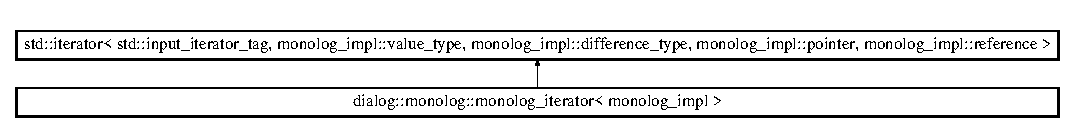
\includegraphics[height=1.339713cm]{classdialog_1_1monolog_1_1monolog__iterator}
\end{center}
\end{figure}
\subsection*{Public Types}
\begin{DoxyCompactItemize}
\item 
\mbox{\Hypertarget{classdialog_1_1monolog_1_1monolog__iterator_a2e80ff238954336c044562b8636ce2c0}\label{classdialog_1_1monolog_1_1monolog__iterator_a2e80ff238954336c044562b8636ce2c0}} 
typedef monolog\+\_\+impl\+::value\+\_\+type {\bfseries value\+\_\+type}
\item 
\mbox{\Hypertarget{classdialog_1_1monolog_1_1monolog__iterator_a3213d75c72b443179bb606dca240fff1}\label{classdialog_1_1monolog_1_1monolog__iterator_a3213d75c72b443179bb606dca240fff1}} 
typedef monolog\+\_\+impl\+::difference\+\_\+type {\bfseries difference\+\_\+type}
\item 
\mbox{\Hypertarget{classdialog_1_1monolog_1_1monolog__iterator_af8237350c8b12bd085a5cc73a5aed7f1}\label{classdialog_1_1monolog_1_1monolog__iterator_af8237350c8b12bd085a5cc73a5aed7f1}} 
typedef monolog\+\_\+impl\+::pointer {\bfseries pointer}
\item 
\mbox{\Hypertarget{classdialog_1_1monolog_1_1monolog__iterator_ade69ab3ba194147b27dc0b8fe322fdbb}\label{classdialog_1_1monolog_1_1monolog__iterator_ade69ab3ba194147b27dc0b8fe322fdbb}} 
typedef monolog\+\_\+impl\+::reference {\bfseries reference}
\end{DoxyCompactItemize}
\subsection*{Public Member Functions}
\begin{DoxyCompactItemize}
\item 
\mbox{\Hypertarget{classdialog_1_1monolog_1_1monolog__iterator_a889db1621e11a5779674461c63afc43f}\label{classdialog_1_1monolog_1_1monolog__iterator_a889db1621e11a5779674461c63afc43f}} 
{\bfseries monolog\+\_\+iterator} (const monolog\+\_\+impl $\ast$impl, size\+\_\+t pos)
\item 
\mbox{\Hypertarget{classdialog_1_1monolog_1_1monolog__iterator_ae4c69a3fba206599055287abba1ee29f}\label{classdialog_1_1monolog_1_1monolog__iterator_ae4c69a3fba206599055287abba1ee29f}} 
reference {\bfseries operator$\ast$} () const
\item 
\mbox{\Hypertarget{classdialog_1_1monolog_1_1monolog__iterator_ac4786a3cd9b8a2b418d4e24d37374938}\label{classdialog_1_1monolog_1_1monolog__iterator_ac4786a3cd9b8a2b418d4e24d37374938}} 
pointer {\bfseries operator-\/$>$} () const
\item 
\mbox{\Hypertarget{classdialog_1_1monolog_1_1monolog__iterator_a11b03414f73b0805aaecddfb9af28819}\label{classdialog_1_1monolog_1_1monolog__iterator_a11b03414f73b0805aaecddfb9af28819}} 
\hyperlink{classdialog_1_1monolog_1_1monolog__iterator}{monolog\+\_\+iterator} \& {\bfseries operator++} ()
\item 
\mbox{\Hypertarget{classdialog_1_1monolog_1_1monolog__iterator_ab3eb2c7f0297bfd7b3a06a7136879e51}\label{classdialog_1_1monolog_1_1monolog__iterator_ab3eb2c7f0297bfd7b3a06a7136879e51}} 
\hyperlink{classdialog_1_1monolog_1_1monolog__iterator}{monolog\+\_\+iterator} {\bfseries operator++} (int)
\item 
\mbox{\Hypertarget{classdialog_1_1monolog_1_1monolog__iterator_a492c37ede0dc453baa10d7117294c960}\label{classdialog_1_1monolog_1_1monolog__iterator_a492c37ede0dc453baa10d7117294c960}} 
bool {\bfseries operator==} (\hyperlink{classdialog_1_1monolog_1_1monolog__iterator}{monolog\+\_\+iterator} other) const
\item 
\mbox{\Hypertarget{classdialog_1_1monolog_1_1monolog__iterator_a5d3c1f7726755d6401e47c73eb79d84f}\label{classdialog_1_1monolog_1_1monolog__iterator_a5d3c1f7726755d6401e47c73eb79d84f}} 
bool {\bfseries operator!=} (\hyperlink{classdialog_1_1monolog_1_1monolog__iterator}{monolog\+\_\+iterator} other) const
\item 
\mbox{\Hypertarget{classdialog_1_1monolog_1_1monolog__iterator_a9062af90996e2d38b005017b2d7f3183}\label{classdialog_1_1monolog_1_1monolog__iterator_a9062af90996e2d38b005017b2d7f3183}} 
\hyperlink{classdialog_1_1monolog_1_1monolog__iterator}{monolog\+\_\+iterator} \& {\bfseries operator=} (const \hyperlink{classdialog_1_1monolog_1_1monolog__iterator}{monolog\+\_\+iterator} \&other)
\end{DoxyCompactItemize}


\subsection{Detailed Description}
\subsubsection*{template$<$typename monolog\+\_\+impl$>$\newline
class dialog\+::monolog\+::monolog\+\_\+iterator$<$ monolog\+\_\+impl $>$}

Iterator for monologs. 

The documentation for this class was generated from the following file\+:\begin{DoxyCompactItemize}
\item 
/\+Users/neil/\+Documents/\+Berkeley/research/dialog/libdialog/dialog/monolog\+\_\+exp2.\+h\end{DoxyCompactItemize}

\hypertarget{classdialog_1_1monolog_1_1monolog__linear}{}\section{dialog\+:\+:monolog\+:\+:monolog\+\_\+linear$<$ T, M\+A\+X\+\_\+\+B\+L\+O\+C\+KS, B\+L\+O\+C\+K\+\_\+\+S\+I\+ZE, B\+U\+F\+F\+E\+R\+\_\+\+S\+I\+ZE $>$ Class Template Reference}
\label{classdialog_1_1monolog_1_1monolog__linear}\index{dialog\+::monolog\+::monolog\+\_\+linear$<$ T, M\+A\+X\+\_\+\+B\+L\+O\+C\+K\+S, B\+L\+O\+C\+K\+\_\+\+S\+I\+Z\+E, B\+U\+F\+F\+E\+R\+\_\+\+S\+I\+Z\+E $>$@{dialog\+::monolog\+::monolog\+\_\+linear$<$ T, M\+A\+X\+\_\+\+B\+L\+O\+C\+K\+S, B\+L\+O\+C\+K\+\_\+\+S\+I\+Z\+E, B\+U\+F\+F\+E\+R\+\_\+\+S\+I\+Z\+E $>$}}
Inheritance diagram for dialog\+:\+:monolog\+:\+:monolog\+\_\+linear$<$ T, M\+A\+X\+\_\+\+B\+L\+O\+C\+KS, B\+L\+O\+C\+K\+\_\+\+S\+I\+ZE, B\+U\+F\+F\+E\+R\+\_\+\+S\+I\+ZE $>$\+:\begin{figure}[H]
\begin{center}
\leavevmode
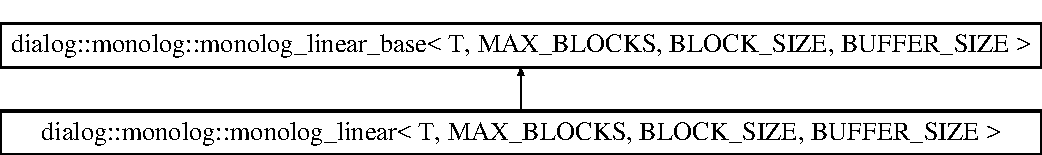
\includegraphics[height=2.000000cm]{classdialog_1_1monolog_1_1monolog__linear}
\end{center}
\end{figure}
\subsection*{Public Types}
\begin{DoxyCompactItemize}
\item 
\mbox{\Hypertarget{classdialog_1_1monolog_1_1monolog__linear_a4c35060b9db227ae41d53adfbbf98754}\label{classdialog_1_1monolog_1_1monolog__linear_a4c35060b9db227ae41d53adfbbf98754}} 
typedef size\+\_\+t {\bfseries size\+\_\+type}
\item 
\mbox{\Hypertarget{classdialog_1_1monolog_1_1monolog__linear_a600bbf1ecd2906db568b9601ff0800ba}\label{classdialog_1_1monolog_1_1monolog__linear_a600bbf1ecd2906db568b9601ff0800ba}} 
typedef size\+\_\+t {\bfseries pos\+\_\+type}
\item 
\mbox{\Hypertarget{classdialog_1_1monolog_1_1monolog__linear_ab86d46ab870789b1940451d6a6fa198b}\label{classdialog_1_1monolog_1_1monolog__linear_ab86d46ab870789b1940451d6a6fa198b}} 
typedef T {\bfseries value\+\_\+type}
\item 
\mbox{\Hypertarget{classdialog_1_1monolog_1_1monolog__linear_aaffd9ed6b9cd8097fe4f60e8259a7445}\label{classdialog_1_1monolog_1_1monolog__linear_aaffd9ed6b9cd8097fe4f60e8259a7445}} 
typedef T {\bfseries difference\+\_\+type}
\item 
\mbox{\Hypertarget{classdialog_1_1monolog_1_1monolog__linear_a874cdbb0087e094c8b705a30d8b1e1f6}\label{classdialog_1_1monolog_1_1monolog__linear_a874cdbb0087e094c8b705a30d8b1e1f6}} 
typedef T $\ast$ {\bfseries pointer}
\item 
\mbox{\Hypertarget{classdialog_1_1monolog_1_1monolog__linear_afe41d924217028d48cb7403b192cc59a}\label{classdialog_1_1monolog_1_1monolog__linear_afe41d924217028d48cb7403b192cc59a}} 
typedef T {\bfseries reference}
\item 
\mbox{\Hypertarget{classdialog_1_1monolog_1_1monolog__linear_ac7f07437eb9d7766c6d440c2bf885d2d}\label{classdialog_1_1monolog_1_1monolog__linear_ac7f07437eb9d7766c6d440c2bf885d2d}} 
typedef \hyperlink{classdialog_1_1monolog_1_1monolog__iterator}{monolog\+\_\+iterator}$<$ \hyperlink{classdialog_1_1monolog_1_1monolog__linear}{monolog\+\_\+linear}$<$ T, M\+A\+X\+\_\+\+B\+L\+O\+C\+KS, B\+L\+O\+C\+K\+\_\+\+S\+I\+ZE, B\+U\+F\+F\+E\+R\+\_\+\+S\+I\+ZE $>$ $>$ {\bfseries iterator}
\item 
\mbox{\Hypertarget{classdialog_1_1monolog_1_1monolog__linear_ad8d50968cecff583da2055963fe82d6c}\label{classdialog_1_1monolog_1_1monolog__linear_ad8d50968cecff583da2055963fe82d6c}} 
typedef \hyperlink{classdialog_1_1monolog_1_1monolog__iterator}{monolog\+\_\+iterator}$<$ \hyperlink{classdialog_1_1monolog_1_1monolog__linear}{monolog\+\_\+linear}$<$ T, M\+A\+X\+\_\+\+B\+L\+O\+C\+KS, B\+L\+O\+C\+K\+\_\+\+S\+I\+ZE, B\+U\+F\+F\+E\+R\+\_\+\+S\+I\+ZE $>$ $>$ {\bfseries const\+\_\+iterator}
\end{DoxyCompactItemize}
\subsection*{Public Member Functions}
\begin{DoxyCompactItemize}
\item 
\mbox{\Hypertarget{classdialog_1_1monolog_1_1monolog__linear_a4a41bea32990a839ad4b5cf335637332}\label{classdialog_1_1monolog_1_1monolog__linear_a4a41bea32990a839ad4b5cf335637332}} 
{\bfseries monolog\+\_\+linear} (const std\+::string \&name, const std\+::string \&data\+\_\+path, const \hyperlink{structdialog_1_1storage_1_1storage__mode}{storage\+::storage\+\_\+mode} \&storage=storage\+::\+I\+N\+\_\+\+M\+E\+M\+O\+RY)
\item 
\mbox{\Hypertarget{classdialog_1_1monolog_1_1monolog__linear_afebe4e6129d5d71e8dc529047d5acae2}\label{classdialog_1_1monolog_1_1monolog__linear_afebe4e6129d5d71e8dc529047d5acae2}} 
size\+\_\+t {\bfseries push\+\_\+back} (const T \&val)
\item 
\mbox{\Hypertarget{classdialog_1_1monolog_1_1monolog__linear_adcc106b67ab06eeb8c8283bc549f2598}\label{classdialog_1_1monolog_1_1monolog__linear_adcc106b67ab06eeb8c8283bc549f2598}} 
size\+\_\+t {\bfseries push\+\_\+back\+\_\+range} (const T \&start, const T \&end)
\item 
\mbox{\Hypertarget{classdialog_1_1monolog_1_1monolog__linear_aa77371cef9ef60420c54c196cb1c0c4d}\label{classdialog_1_1monolog_1_1monolog__linear_aa77371cef9ef60420c54c196cb1c0c4d}} 
size\+\_\+t {\bfseries append} (const T $\ast$\hyperlink{structdialog_1_1data}{data}, size\+\_\+t len)
\item 
\mbox{\Hypertarget{classdialog_1_1monolog_1_1monolog__linear_a78ba15a7a6d22fc693b90be95a986278}\label{classdialog_1_1monolog_1_1monolog__linear_a78ba15a7a6d22fc693b90be95a986278}} 
size\+\_\+t {\bfseries reserve} (size\+\_\+t len)
\item 
\mbox{\Hypertarget{classdialog_1_1monolog_1_1monolog__linear_a40eb17ee39bb8cb2cf920102f2ecb7bf}\label{classdialog_1_1monolog_1_1monolog__linear_a40eb17ee39bb8cb2cf920102f2ecb7bf}} 
const T \& {\bfseries at} (size\+\_\+t idx) const
\item 
\mbox{\Hypertarget{classdialog_1_1monolog_1_1monolog__linear_a3e65b10aca673058e344c10022dca01f}\label{classdialog_1_1monolog_1_1monolog__linear_a3e65b10aca673058e344c10022dca01f}} 
size\+\_\+t {\bfseries size} () const
\item 
\mbox{\Hypertarget{classdialog_1_1monolog_1_1monolog__linear_af294efb6d41e8f0449f5fd256c5a0af4}\label{classdialog_1_1monolog_1_1monolog__linear_af294efb6d41e8f0449f5fd256c5a0af4}} 
\hyperlink{classdialog_1_1monolog_1_1monolog__iterator}{iterator} {\bfseries begin} () const
\item 
\mbox{\Hypertarget{classdialog_1_1monolog_1_1monolog__linear_aa13bd42e4ad0fe5b8c8e645b367d161f}\label{classdialog_1_1monolog_1_1monolog__linear_aa13bd42e4ad0fe5b8c8e645b367d161f}} 
\hyperlink{classdialog_1_1monolog_1_1monolog__iterator}{iterator} {\bfseries end} () const
\end{DoxyCompactItemize}
\subsection*{Additional Inherited Members}


The documentation for this class was generated from the following file\+:\begin{DoxyCompactItemize}
\item 
/\+Users/neil/\+Documents/\+Berkeley/research/dialog/libdialog/dialog/monolog\+\_\+linear.\+h\end{DoxyCompactItemize}

\hypertarget{classdialog_1_1monolog_1_1monolog__linear__base}{}\section{dialog\+:\+:monolog\+:\+:monolog\+\_\+linear\+\_\+base$<$ T, M\+A\+X\+\_\+\+B\+L\+O\+C\+KS, B\+L\+O\+C\+K\+\_\+\+S\+I\+ZE, B\+U\+F\+F\+E\+R\+\_\+\+S\+I\+ZE $>$ Class Template Reference}
\label{classdialog_1_1monolog_1_1monolog__linear__base}\index{dialog\+::monolog\+::monolog\+\_\+linear\+\_\+base$<$ T, M\+A\+X\+\_\+\+B\+L\+O\+C\+K\+S, B\+L\+O\+C\+K\+\_\+\+S\+I\+Z\+E, B\+U\+F\+F\+E\+R\+\_\+\+S\+I\+Z\+E $>$@{dialog\+::monolog\+::monolog\+\_\+linear\+\_\+base$<$ T, M\+A\+X\+\_\+\+B\+L\+O\+C\+K\+S, B\+L\+O\+C\+K\+\_\+\+S\+I\+Z\+E, B\+U\+F\+F\+E\+R\+\_\+\+S\+I\+Z\+E $>$}}
Inheritance diagram for dialog\+:\+:monolog\+:\+:monolog\+\_\+linear\+\_\+base$<$ T, M\+A\+X\+\_\+\+B\+L\+O\+C\+KS, B\+L\+O\+C\+K\+\_\+\+S\+I\+ZE, B\+U\+F\+F\+E\+R\+\_\+\+S\+I\+ZE $>$\+:\begin{figure}[H]
\begin{center}
\leavevmode
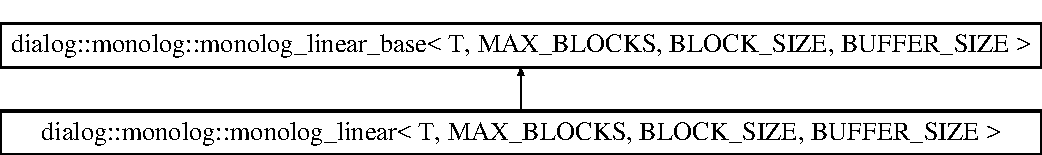
\includegraphics[height=2.000000cm]{classdialog_1_1monolog_1_1monolog__linear__base}
\end{center}
\end{figure}
\subsection*{Public Member Functions}
\begin{DoxyCompactItemize}
\item 
\mbox{\Hypertarget{classdialog_1_1monolog_1_1monolog__linear__base_ad8c76402bc404f2f39fa5675fdf0f0c3}\label{classdialog_1_1monolog_1_1monolog__linear__base_ad8c76402bc404f2f39fa5675fdf0f0c3}} 
{\bfseries monolog\+\_\+linear\+\_\+base} (const std\+::string \&name, const std\+::string \&data\+\_\+path, const \hyperlink{structdialog_1_1storage_1_1storage__mode}{storage\+::storage\+\_\+mode} \&storage)
\item 
\mbox{\Hypertarget{classdialog_1_1monolog_1_1monolog__linear__base_afd25fba29a97be9f4ca88f2b8f6bda81}\label{classdialog_1_1monolog_1_1monolog__linear__base_afd25fba29a97be9f4ca88f2b8f6bda81}} 
void {\bfseries init} (const std\+::string \&name, const std\+::string \&data\+\_\+path, const \hyperlink{structdialog_1_1storage_1_1storage__mode}{storage\+::storage\+\_\+mode} \&storage)
\item 
\mbox{\Hypertarget{classdialog_1_1monolog_1_1monolog__linear__base_ae381905913522b2049e30e8906e58256}\label{classdialog_1_1monolog_1_1monolog__linear__base_ae381905913522b2049e30e8906e58256}} 
std\+::string {\bfseries name} () const
\item 
\mbox{\Hypertarget{classdialog_1_1monolog_1_1monolog__linear__base_aa2fb2303ceeb3c414253887141a5d5ad}\label{classdialog_1_1monolog_1_1monolog__linear__base_aa2fb2303ceeb3c414253887141a5d5ad}} 
std\+::string {\bfseries data\+\_\+path} () const
\item 
\mbox{\Hypertarget{classdialog_1_1monolog_1_1monolog__linear__base_ab47c32ca7520b3f2013668aa944155b9}\label{classdialog_1_1monolog_1_1monolog__linear__base_ab47c32ca7520b3f2013668aa944155b9}} 
void {\bfseries ensure\+\_\+alloc} (size\+\_\+t idx1, size\+\_\+t idx2)
\item 
\mbox{\Hypertarget{classdialog_1_1monolog_1_1monolog__linear__base_a61b4205f5c566b48a9bb39193da48695}\label{classdialog_1_1monolog_1_1monolog__linear__base_a61b4205f5c566b48a9bb39193da48695}} 
void {\bfseries set} (size\+\_\+t idx, const T \&val)
\item 
\mbox{\Hypertarget{classdialog_1_1monolog_1_1monolog__linear__base_a2845c0248840b7af62b5534c037db58c}\label{classdialog_1_1monolog_1_1monolog__linear__base_a2845c0248840b7af62b5534c037db58c}} 
void {\bfseries set\+\_\+unsafe} (size\+\_\+t idx, const T val)
\item 
\mbox{\Hypertarget{classdialog_1_1monolog_1_1monolog__linear__base_a894a91791dcb1837e583182b66271d3d}\label{classdialog_1_1monolog_1_1monolog__linear__base_a894a91791dcb1837e583182b66271d3d}} 
void {\bfseries write} (size\+\_\+t offset, const T $\ast$\hyperlink{structdialog_1_1data}{data}, size\+\_\+t len)
\item 
\mbox{\Hypertarget{classdialog_1_1monolog_1_1monolog__linear__base_a4df464bcedf7033602bc140d193bb2f8}\label{classdialog_1_1monolog_1_1monolog__linear__base_a4df464bcedf7033602bc140d193bb2f8}} 
void {\bfseries write\+\_\+unsafe} (size\+\_\+t offset, const T $\ast$\hyperlink{structdialog_1_1data}{data}, size\+\_\+t len)
\item 
\mbox{\Hypertarget{classdialog_1_1monolog_1_1monolog__linear__base_aa2188965d4fb188934b11148aed06b55}\label{classdialog_1_1monolog_1_1monolog__linear__base_aa2188965d4fb188934b11148aed06b55}} 
void {\bfseries flush} (size\+\_\+t offset, size\+\_\+t len)
\item 
\mbox{\Hypertarget{classdialog_1_1monolog_1_1monolog__linear__base_aeac00c4aa51b89014a332bbd5bcb588f}\label{classdialog_1_1monolog_1_1monolog__linear__base_aeac00c4aa51b89014a332bbd5bcb588f}} 
const T \& {\bfseries get} (size\+\_\+t idx) const
\item 
\mbox{\Hypertarget{classdialog_1_1monolog_1_1monolog__linear__base_a5ff1e356bb090c7d348bc3c75099853e}\label{classdialog_1_1monolog_1_1monolog__linear__base_a5ff1e356bb090c7d348bc3c75099853e}} 
void {\bfseries read} (size\+\_\+t offset, T $\ast$\hyperlink{structdialog_1_1data}{data}, size\+\_\+t len) const
\item 
\mbox{\Hypertarget{classdialog_1_1monolog_1_1monolog__linear__base_a72cd744e31249156eb64f6b50189f0c7}\label{classdialog_1_1monolog_1_1monolog__linear__base_a72cd744e31249156eb64f6b50189f0c7}} 
T \& {\bfseries operator\mbox{[}$\,$\mbox{]}} (size\+\_\+t idx)
\item 
\mbox{\Hypertarget{classdialog_1_1monolog_1_1monolog__linear__base_a3344aa0111540914577b615aaee9d463}\label{classdialog_1_1monolog_1_1monolog__linear__base_a3344aa0111540914577b615aaee9d463}} 
void $\ast$ {\bfseries ptr} (size\+\_\+t offset)
\item 
\mbox{\Hypertarget{classdialog_1_1monolog_1_1monolog__linear__base_aec9a6582f7431a499db700ce26984281}\label{classdialog_1_1monolog_1_1monolog__linear__base_aec9a6582f7431a499db700ce26984281}} 
void $\ast$ {\bfseries ptr} (size\+\_\+t offset) const
\item 
\mbox{\Hypertarget{classdialog_1_1monolog_1_1monolog__linear__base_aaab4f77900ec6e9a090828eb14753cdd}\label{classdialog_1_1monolog_1_1monolog__linear__base_aaab4f77900ec6e9a090828eb14753cdd}} 
void $\ast$ {\bfseries cptr} (size\+\_\+t offset) const
\item 
\mbox{\Hypertarget{classdialog_1_1monolog_1_1monolog__linear__base_a9d6916b45b86ee569c7b9f1d71f1ab2b}\label{classdialog_1_1monolog_1_1monolog__linear__base_a9d6916b45b86ee569c7b9f1d71f1ab2b}} 
size\+\_\+t {\bfseries storage\+\_\+size} () const
\end{DoxyCompactItemize}
\subsection*{Protected Attributes}
\begin{DoxyCompactItemize}
\item 
\mbox{\Hypertarget{classdialog_1_1monolog_1_1monolog__linear__base_a65545bd6b412019ba9ca2031d596a26a}\label{classdialog_1_1monolog_1_1monolog__linear__base_a65545bd6b412019ba9ca2031d596a26a}} 
std\+::string {\bfseries name\+\_\+}
\item 
\mbox{\Hypertarget{classdialog_1_1monolog_1_1monolog__linear__base_ae5f8ae470de3c355febbaf1c793d9164}\label{classdialog_1_1monolog_1_1monolog__linear__base_ae5f8ae470de3c355febbaf1c793d9164}} 
std\+::string {\bfseries data\+\_\+path\+\_\+}
\item 
\mbox{\Hypertarget{classdialog_1_1monolog_1_1monolog__linear__base_a53b03175e1a621804ce4b54ce0b5b049}\label{classdialog_1_1monolog_1_1monolog__linear__base_a53b03175e1a621804ce4b54ce0b5b049}} 
std\+::array$<$ \hyperlink{classdialog_1_1monolog_1_1monolog__block}{monolog\+\_\+block}$<$ T, B\+U\+F\+F\+E\+R\+\_\+\+S\+I\+ZE $>$, M\+A\+X\+\_\+\+B\+L\+O\+C\+KS $>$ {\bfseries blocks\+\_\+}
\end{DoxyCompactItemize}


The documentation for this class was generated from the following file\+:\begin{DoxyCompactItemize}
\item 
/\+Users/neil/\+Documents/\+Berkeley/research/dialog/libdialog/dialog/monolog\+\_\+linear.\+h\end{DoxyCompactItemize}

\hypertarget{classdialog_1_1mutable__value}{}\section{dialog\+:\+:mutable\+\_\+value Class Reference}
\label{classdialog_1_1mutable__value}\index{dialog\+::mutable\+\_\+value@{dialog\+::mutable\+\_\+value}}
Inheritance diagram for dialog\+:\+:mutable\+\_\+value\+:\begin{figure}[H]
\begin{center}
\leavevmode
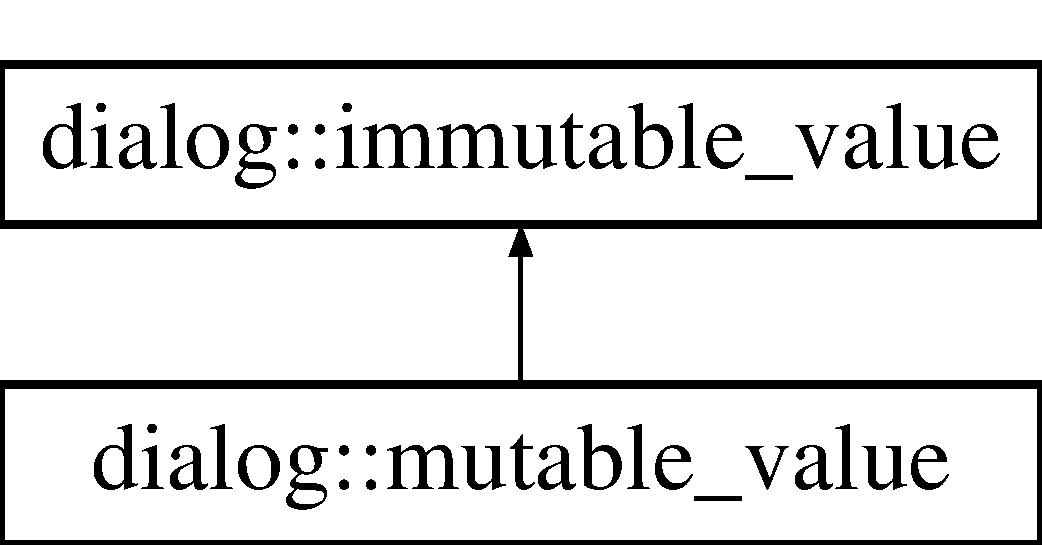
\includegraphics[height=2.000000cm]{classdialog_1_1mutable__value}
\end{center}
\end{figure}
\subsection*{Public Member Functions}
\begin{DoxyCompactItemize}
\item 
\mbox{\Hypertarget{classdialog_1_1mutable__value_af695c5b26c447cdeac8b5e3a78fff53d}\label{classdialog_1_1mutable__value_af695c5b26c447cdeac8b5e3a78fff53d}} 
{\bfseries mutable\+\_\+value} (\hyperlink{structdialog_1_1data__type}{data\+\_\+type} type=N\+O\+N\+E\+\_\+\+T\+Y\+PE)
\item 
\mbox{\Hypertarget{classdialog_1_1mutable__value_a2f29974b74f4075f5518970828f49935}\label{classdialog_1_1mutable__value_a2f29974b74f4075f5518970828f49935}} 
{\bfseries mutable\+\_\+value} (const \hyperlink{structdialog_1_1data__type}{data\+\_\+type} \&type, const void $\ast$value)
\item 
\mbox{\Hypertarget{classdialog_1_1mutable__value_acbd3f344366cc35d75dc83783cb58c22}\label{classdialog_1_1mutable__value_acbd3f344366cc35d75dc83783cb58c22}} 
{\bfseries mutable\+\_\+value} (bool value)
\item 
\mbox{\Hypertarget{classdialog_1_1mutable__value_a21f1039a8b21ef42b795c99ece668b18}\label{classdialog_1_1mutable__value_a21f1039a8b21ef42b795c99ece668b18}} 
{\bfseries mutable\+\_\+value} (int8\+\_\+t value)
\item 
\mbox{\Hypertarget{classdialog_1_1mutable__value_a243c36a8bcaff0efb48078d1da0ce0e8}\label{classdialog_1_1mutable__value_a243c36a8bcaff0efb48078d1da0ce0e8}} 
{\bfseries mutable\+\_\+value} (int16\+\_\+t value)
\item 
\mbox{\Hypertarget{classdialog_1_1mutable__value_ad15529ed7c5e43c79afea685979d329f}\label{classdialog_1_1mutable__value_ad15529ed7c5e43c79afea685979d329f}} 
{\bfseries mutable\+\_\+value} (int32\+\_\+t value)
\item 
\mbox{\Hypertarget{classdialog_1_1mutable__value_a1b691434877e4c601aa4b20d28536888}\label{classdialog_1_1mutable__value_a1b691434877e4c601aa4b20d28536888}} 
{\bfseries mutable\+\_\+value} (int64\+\_\+t value)
\item 
\mbox{\Hypertarget{classdialog_1_1mutable__value_ab95cf82769c1bc446ce0bc0a9cdc9c13}\label{classdialog_1_1mutable__value_ab95cf82769c1bc446ce0bc0a9cdc9c13}} 
{\bfseries mutable\+\_\+value} (float value)
\item 
\mbox{\Hypertarget{classdialog_1_1mutable__value_a485a10a14e3ebb08240d88a715d52e9f}\label{classdialog_1_1mutable__value_a485a10a14e3ebb08240d88a715d52e9f}} 
{\bfseries mutable\+\_\+value} (double value)
\item 
\mbox{\Hypertarget{classdialog_1_1mutable__value_a942994748f636c383f1ab3897326a4e0}\label{classdialog_1_1mutable__value_a942994748f636c383f1ab3897326a4e0}} 
{\bfseries mutable\+\_\+value} (const std\+::string \&str)
\item 
\mbox{\Hypertarget{classdialog_1_1mutable__value_a074757ebe0c418a29855aa0527ae80ce}\label{classdialog_1_1mutable__value_a074757ebe0c418a29855aa0527ae80ce}} 
{\bfseries mutable\+\_\+value} (const \hyperlink{classdialog_1_1immutable__value}{immutable\+\_\+value} \&other)
\item 
\mbox{\Hypertarget{classdialog_1_1mutable__value_a23e366956a4881b42eeede3c9a6af94f}\label{classdialog_1_1mutable__value_a23e366956a4881b42eeede3c9a6af94f}} 
{\bfseries mutable\+\_\+value} (const \hyperlink{classdialog_1_1mutable__value}{mutable\+\_\+value} \&other)
\item 
\mbox{\Hypertarget{classdialog_1_1mutable__value_a29c5f9064177c8c673306e7f3b09acdf}\label{classdialog_1_1mutable__value_a29c5f9064177c8c673306e7f3b09acdf}} 
{\bfseries mutable\+\_\+value} (\hyperlink{classdialog_1_1mutable__value}{mutable\+\_\+value} \&\&other)
\item 
\mbox{\Hypertarget{classdialog_1_1mutable__value_aba4b910ac731fb8dbbda211fa918c443}\label{classdialog_1_1mutable__value_aba4b910ac731fb8dbbda211fa918c443}} 
\hyperlink{classdialog_1_1immutable__value}{immutable\+\_\+value} {\bfseries copy} () const
\item 
\mbox{\Hypertarget{classdialog_1_1mutable__value_a0fcb8afa5afa9d4c3384035cdba66d32}\label{classdialog_1_1mutable__value_a0fcb8afa5afa9d4c3384035cdba66d32}} 
\hyperlink{classdialog_1_1mutable__value}{mutable\+\_\+value} \& {\bfseries operator=} (const \hyperlink{classdialog_1_1immutable__value}{immutable\+\_\+value} \&other)
\item 
\mbox{\Hypertarget{classdialog_1_1mutable__value_a513fe862f5ed5b0fc3cb37513b1b80a1}\label{classdialog_1_1mutable__value_a513fe862f5ed5b0fc3cb37513b1b80a1}} 
\hyperlink{classdialog_1_1mutable__value}{mutable\+\_\+value} \& {\bfseries operator=} (const \hyperlink{classdialog_1_1mutable__value}{mutable\+\_\+value} \&other)
\item 
\mbox{\Hypertarget{classdialog_1_1mutable__value_a42b1a9dc82410c8b082950e4238cdbed}\label{classdialog_1_1mutable__value_a42b1a9dc82410c8b082950e4238cdbed}} 
\hyperlink{classdialog_1_1mutable__value}{mutable\+\_\+value} \& {\bfseries operator=} (\hyperlink{classdialog_1_1mutable__value}{mutable\+\_\+value} \&\&other)
\end{DoxyCompactItemize}
\subsection*{Static Public Member Functions}
\begin{DoxyCompactItemize}
\item 
\mbox{\Hypertarget{classdialog_1_1mutable__value_a81096a1163464473f3fcb346644f1631}\label{classdialog_1_1mutable__value_a81096a1163464473f3fcb346644f1631}} 
static \hyperlink{classdialog_1_1mutable__value}{mutable\+\_\+value} {\bfseries parse} (const std\+::string \&str, const \hyperlink{structdialog_1_1data__type}{data\+\_\+type} \&type)
\item 
\mbox{\Hypertarget{classdialog_1_1mutable__value_a53e69a0ccf0aef556db129313fc120d1}\label{classdialog_1_1mutable__value_a53e69a0ccf0aef556db129313fc120d1}} 
static \hyperlink{classdialog_1_1mutable__value}{mutable\+\_\+value} {\bfseries unaryop} (unaryop\+\_\+id id, const \hyperlink{classdialog_1_1immutable__value}{immutable\+\_\+value} \&n)
\item 
\mbox{\Hypertarget{classdialog_1_1mutable__value_ac0913ac341698f2cef43a3804f780bde}\label{classdialog_1_1mutable__value_ac0913ac341698f2cef43a3804f780bde}} 
static \hyperlink{classdialog_1_1mutable__value}{mutable\+\_\+value} {\bfseries binaryop} (binaryop\+\_\+id id, const \hyperlink{classdialog_1_1immutable__value}{immutable\+\_\+value} \&first, const \hyperlink{classdialog_1_1immutable__value}{immutable\+\_\+value} \&second)
\end{DoxyCompactItemize}
\subsection*{Friends}
\begin{DoxyCompactItemize}
\item 
\mbox{\Hypertarget{classdialog_1_1mutable__value_a00adf7bda6ac2a310d53e7ddbe990dc9}\label{classdialog_1_1mutable__value_a00adf7bda6ac2a310d53e7ddbe990dc9}} 
\hyperlink{classdialog_1_1mutable__value}{mutable\+\_\+value} {\bfseries operator-\/} (const \hyperlink{classdialog_1_1immutable__value}{immutable\+\_\+value} \&n)
\item 
\mbox{\Hypertarget{classdialog_1_1mutable__value_a51cec9f0cc1f6416577459cd260e2221}\label{classdialog_1_1mutable__value_a51cec9f0cc1f6416577459cd260e2221}} 
\hyperlink{classdialog_1_1mutable__value}{mutable\+\_\+value} {\bfseries operator+} (const \hyperlink{classdialog_1_1immutable__value}{immutable\+\_\+value} \&n)
\item 
\mbox{\Hypertarget{classdialog_1_1mutable__value_a2405f68fffcf1bf68a332a9680aa0198}\label{classdialog_1_1mutable__value_a2405f68fffcf1bf68a332a9680aa0198}} 
\hyperlink{classdialog_1_1mutable__value}{mutable\+\_\+value} {\bfseries operator$\sim$} (const \hyperlink{classdialog_1_1immutable__value}{immutable\+\_\+value} \&n)
\item 
\mbox{\Hypertarget{classdialog_1_1mutable__value_a2fe0780b8951e996611809cdf531c8e7}\label{classdialog_1_1mutable__value_a2fe0780b8951e996611809cdf531c8e7}} 
\hyperlink{classdialog_1_1mutable__value}{mutable\+\_\+value} {\bfseries operator+} (const \hyperlink{classdialog_1_1immutable__value}{immutable\+\_\+value} \&first, const \hyperlink{classdialog_1_1immutable__value}{immutable\+\_\+value} \&second)
\item 
\mbox{\Hypertarget{classdialog_1_1mutable__value_a1c18bc903370d7cee73614a96ec5f067}\label{classdialog_1_1mutable__value_a1c18bc903370d7cee73614a96ec5f067}} 
\hyperlink{classdialog_1_1mutable__value}{mutable\+\_\+value} {\bfseries operator-\/} (const \hyperlink{classdialog_1_1immutable__value}{immutable\+\_\+value} \&first, const \hyperlink{classdialog_1_1immutable__value}{immutable\+\_\+value} \&second)
\item 
\mbox{\Hypertarget{classdialog_1_1mutable__value_a8a09cfa8690a125b394b1b948b7e13a0}\label{classdialog_1_1mutable__value_a8a09cfa8690a125b394b1b948b7e13a0}} 
\hyperlink{classdialog_1_1mutable__value}{mutable\+\_\+value} {\bfseries operator$\ast$} (const \hyperlink{classdialog_1_1immutable__value}{immutable\+\_\+value} \&first, const \hyperlink{classdialog_1_1immutable__value}{immutable\+\_\+value} \&second)
\item 
\mbox{\Hypertarget{classdialog_1_1mutable__value_aca65e78b0627d39e1d8a5c65f8832f00}\label{classdialog_1_1mutable__value_aca65e78b0627d39e1d8a5c65f8832f00}} 
\hyperlink{classdialog_1_1mutable__value}{mutable\+\_\+value} {\bfseries operator/} (const \hyperlink{classdialog_1_1immutable__value}{immutable\+\_\+value} \&first, const \hyperlink{classdialog_1_1immutable__value}{immutable\+\_\+value} \&second)
\item 
\mbox{\Hypertarget{classdialog_1_1mutable__value_acbe003fe899f51f80bb8ed58a4d2c100}\label{classdialog_1_1mutable__value_acbe003fe899f51f80bb8ed58a4d2c100}} 
\hyperlink{classdialog_1_1mutable__value}{mutable\+\_\+value} {\bfseries operator\%} (const \hyperlink{classdialog_1_1immutable__value}{immutable\+\_\+value} \&first, const \hyperlink{classdialog_1_1immutable__value}{immutable\+\_\+value} \&second)
\item 
\mbox{\Hypertarget{classdialog_1_1mutable__value_a99dd5f11ce5aa06e3309e8e59487fdd5}\label{classdialog_1_1mutable__value_a99dd5f11ce5aa06e3309e8e59487fdd5}} 
\hyperlink{classdialog_1_1mutable__value}{mutable\+\_\+value} {\bfseries operator \&} (const \hyperlink{classdialog_1_1immutable__value}{immutable\+\_\+value} \&first, const \hyperlink{classdialog_1_1immutable__value}{immutable\+\_\+value} \&second)
\item 
\mbox{\Hypertarget{classdialog_1_1mutable__value_a507fc993fbcfcf24603f5ce0569142d9}\label{classdialog_1_1mutable__value_a507fc993fbcfcf24603f5ce0569142d9}} 
\hyperlink{classdialog_1_1mutable__value}{mutable\+\_\+value} {\bfseries operator$\vert$} (const \hyperlink{classdialog_1_1immutable__value}{immutable\+\_\+value} \&first, const \hyperlink{classdialog_1_1immutable__value}{immutable\+\_\+value} \&second)
\item 
\mbox{\Hypertarget{classdialog_1_1mutable__value_a76d916ee2130786f5bf310d7160e23f3}\label{classdialog_1_1mutable__value_a76d916ee2130786f5bf310d7160e23f3}} 
\hyperlink{classdialog_1_1mutable__value}{mutable\+\_\+value} {\bfseries operator$^\wedge$} (const \hyperlink{classdialog_1_1immutable__value}{immutable\+\_\+value} \&first, const \hyperlink{classdialog_1_1immutable__value}{immutable\+\_\+value} \&second)
\item 
\mbox{\Hypertarget{classdialog_1_1mutable__value_ae852f55df61e179c6418835da3da4797}\label{classdialog_1_1mutable__value_ae852f55df61e179c6418835da3da4797}} 
\hyperlink{classdialog_1_1mutable__value}{mutable\+\_\+value} {\bfseries operator$<$$<$} (const \hyperlink{classdialog_1_1immutable__value}{immutable\+\_\+value} \&first, const \hyperlink{classdialog_1_1immutable__value}{immutable\+\_\+value} \&second)
\item 
\mbox{\Hypertarget{classdialog_1_1mutable__value_a61672ff559824ff840d4d766b9ab0719}\label{classdialog_1_1mutable__value_a61672ff559824ff840d4d766b9ab0719}} 
\hyperlink{classdialog_1_1mutable__value}{mutable\+\_\+value} {\bfseries operator$>$$>$} (const \hyperlink{classdialog_1_1immutable__value}{immutable\+\_\+value} \&first, const \hyperlink{classdialog_1_1immutable__value}{immutable\+\_\+value} \&second)
\end{DoxyCompactItemize}
\subsection*{Additional Inherited Members}


The documentation for this class was generated from the following file\+:\begin{DoxyCompactItemize}
\item 
/\+Users/neil/\+Documents/\+Berkeley/research/dialog/libdialog/dialog/mutable\+\_\+value.\+h\end{DoxyCompactItemize}

\hypertarget{structdialog_1_1negation}{}\section{dialog\+:\+:negation Struct Reference}
\label{structdialog_1_1negation}\index{dialog\+::negation@{dialog\+::negation}}


{\ttfamily \#include $<$expression.\+h$>$}

Inheritance diagram for dialog\+:\+:negation\+:\begin{figure}[H]
\begin{center}
\leavevmode
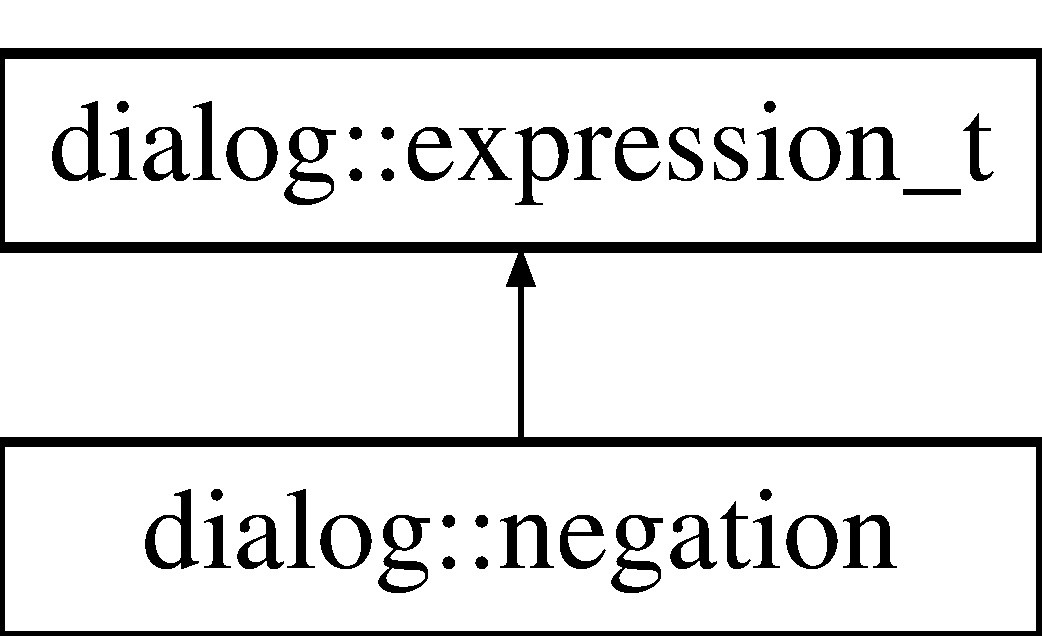
\includegraphics[height=2.000000cm]{structdialog_1_1negation}
\end{center}
\end{figure}
\subsection*{Public Attributes}
\begin{DoxyCompactItemize}
\item 
\mbox{\Hypertarget{structdialog_1_1negation_a8a0b4d4dcf4c1f90808f9fce30ab5b73}\label{structdialog_1_1negation_a8a0b4d4dcf4c1f90808f9fce30ab5b73}} 
\hyperlink{structdialog_1_1expression__t}{expression\+\_\+t} $\ast$ {\bfseries child}
\end{DoxyCompactItemize}
\subsection*{Additional Inherited Members}


\subsection{Detailed Description}
Negation expression. 

The documentation for this struct was generated from the following file\+:\begin{DoxyCompactItemize}
\item 
/\+Users/neil/\+Documents/\+Berkeley/research/dialog/libdialog/dialog/expression.\+h\end{DoxyCompactItemize}

\hypertarget{classdialog_1_1numeric}{}\section{dialog\+:\+:numeric Class Reference}
\label{classdialog_1_1numeric}\index{dialog\+::numeric@{dialog\+::numeric}}
\subsection*{Public Member Functions}
\begin{DoxyCompactItemize}
\item 
\mbox{\Hypertarget{classdialog_1_1numeric_ac863b06cd354cec5cd2d67e83ed147b0}\label{classdialog_1_1numeric_ac863b06cd354cec5cd2d67e83ed147b0}} 
{\bfseries numeric} (\hyperlink{structdialog_1_1data__type}{data\+\_\+type} type)
\item 
\mbox{\Hypertarget{classdialog_1_1numeric_ac932a334ea3d0147b4a787704c7cee3b}\label{classdialog_1_1numeric_ac932a334ea3d0147b4a787704c7cee3b}} 
{\bfseries numeric} (bool val)
\item 
\mbox{\Hypertarget{classdialog_1_1numeric_a350fa2e5d65a75a6d0dd7df3bb095d3d}\label{classdialog_1_1numeric_a350fa2e5d65a75a6d0dd7df3bb095d3d}} 
{\bfseries numeric} (int8\+\_\+t val)
\item 
\mbox{\Hypertarget{classdialog_1_1numeric_ac3e90d058ca9481bb57f4cbeef75374f}\label{classdialog_1_1numeric_ac3e90d058ca9481bb57f4cbeef75374f}} 
{\bfseries numeric} (int16\+\_\+t val)
\item 
\mbox{\Hypertarget{classdialog_1_1numeric_a522d481eb1e2403a80c3b950a10c5b0d}\label{classdialog_1_1numeric_a522d481eb1e2403a80c3b950a10c5b0d}} 
{\bfseries numeric} (int32\+\_\+t val)
\item 
\mbox{\Hypertarget{classdialog_1_1numeric_af74e9daadcfb8cd40315a863e1220947}\label{classdialog_1_1numeric_af74e9daadcfb8cd40315a863e1220947}} 
{\bfseries numeric} (int64\+\_\+t val)
\item 
\mbox{\Hypertarget{classdialog_1_1numeric_a73a23576e3a1523847b729e29a641d6d}\label{classdialog_1_1numeric_a73a23576e3a1523847b729e29a641d6d}} 
{\bfseries numeric} (float val)
\item 
\mbox{\Hypertarget{classdialog_1_1numeric_a48138c620893637ee22dd125049af5da}\label{classdialog_1_1numeric_a48138c620893637ee22dd125049af5da}} 
{\bfseries numeric} (double val)
\item 
\mbox{\Hypertarget{classdialog_1_1numeric_ad29aee52c6db72a3a83e59029a5d9d33}\label{classdialog_1_1numeric_ad29aee52c6db72a3a83e59029a5d9d33}} 
{\bfseries numeric} (const \hyperlink{structdialog_1_1data__type}{data\+\_\+type} \&type, void $\ast$\hyperlink{structdialog_1_1data}{data})
\item 
\mbox{\Hypertarget{classdialog_1_1numeric_ae051a0ba9dc905a91a8c21e7e04f8323}\label{classdialog_1_1numeric_ae051a0ba9dc905a91a8c21e7e04f8323}} 
{\bfseries numeric} (const \hyperlink{classdialog_1_1immutable__value}{immutable\+\_\+value} \&val)
\item 
\mbox{\Hypertarget{classdialog_1_1numeric_aa4cffc0219b07bba63ee1e735215ddc8}\label{classdialog_1_1numeric_aa4cffc0219b07bba63ee1e735215ddc8}} 
\hyperlink{structdialog_1_1data}{data} {\bfseries to\+\_\+data} () const
\item 
\mbox{\Hypertarget{classdialog_1_1numeric_a3574bf3a7c6d5f525b93baf5b8f4f80d}\label{classdialog_1_1numeric_a3574bf3a7c6d5f525b93baf5b8f4f80d}} 
\hyperlink{structdialog_1_1data__type}{data\+\_\+type} const  \& {\bfseries type} () const
\item 
\mbox{\Hypertarget{classdialog_1_1numeric_a6bae3d300bc27d5897b10681ca5f8427}\label{classdialog_1_1numeric_a6bae3d300bc27d5897b10681ca5f8427}} 
\hyperlink{classdialog_1_1numeric}{numeric} \& {\bfseries operator=} (const \hyperlink{classdialog_1_1immutable__value}{immutable\+\_\+value} \&other)
\item 
\mbox{\Hypertarget{classdialog_1_1numeric_a1d9cce706335fce2662c770ab2db27db}\label{classdialog_1_1numeric_a1d9cce706335fce2662c770ab2db27db}} 
\hyperlink{classdialog_1_1numeric}{numeric} \& {\bfseries operator=} (bool value)
\item 
\mbox{\Hypertarget{classdialog_1_1numeric_ae5d060b45ce0dfda6991e39eb005a702}\label{classdialog_1_1numeric_ae5d060b45ce0dfda6991e39eb005a702}} 
\hyperlink{classdialog_1_1numeric}{numeric} \& {\bfseries operator=} (int8\+\_\+t value)
\item 
\mbox{\Hypertarget{classdialog_1_1numeric_a55fdd2e8c392e96cb9e43e200689ad2f}\label{classdialog_1_1numeric_a55fdd2e8c392e96cb9e43e200689ad2f}} 
\hyperlink{classdialog_1_1numeric}{numeric} \& {\bfseries operator=} (int16\+\_\+t value)
\item 
\mbox{\Hypertarget{classdialog_1_1numeric_a7fb02be82d2ba9509182e3d780d6ec39}\label{classdialog_1_1numeric_a7fb02be82d2ba9509182e3d780d6ec39}} 
\hyperlink{classdialog_1_1numeric}{numeric} \& {\bfseries operator=} (int32\+\_\+t value)
\item 
\mbox{\Hypertarget{classdialog_1_1numeric_a9db3cbca3382972629efbd796c43794c}\label{classdialog_1_1numeric_a9db3cbca3382972629efbd796c43794c}} 
\hyperlink{classdialog_1_1numeric}{numeric} \& {\bfseries operator=} (int64\+\_\+t value)
\item 
\mbox{\Hypertarget{classdialog_1_1numeric_a71ab0faa34a90868535344f4fff01b7d}\label{classdialog_1_1numeric_a71ab0faa34a90868535344f4fff01b7d}} 
\hyperlink{classdialog_1_1numeric}{numeric} \& {\bfseries operator=} (float value)
\item 
\mbox{\Hypertarget{classdialog_1_1numeric_a59e33c522912527704f4f71634ee1a76}\label{classdialog_1_1numeric_a59e33c522912527704f4f71634ee1a76}} 
\hyperlink{classdialog_1_1numeric}{numeric} \& {\bfseries operator=} (double value)
\item 
\mbox{\Hypertarget{classdialog_1_1numeric_af419125dfd9391249aab3d078f25520d}\label{classdialog_1_1numeric_af419125dfd9391249aab3d078f25520d}} 
{\footnotesize template$<$typename T , typename std\+::enable\+\_\+if$<$ std\+::is\+\_\+integral$<$ T $>$\+::value$\vert$$\vert$std\+::is\+\_\+floating\+\_\+point$<$ T $>$\+::value, T $>$\+::type $\ast$  = nullptr$>$ }\\T \& {\bfseries as} ()
\item 
\mbox{\Hypertarget{classdialog_1_1numeric_ad23a353a377901b005167816d6c36bbe}\label{classdialog_1_1numeric_ad23a353a377901b005167816d6c36bbe}} 
{\footnotesize template$<$typename T , typename std\+::enable\+\_\+if$<$ std\+::is\+\_\+integral$<$ T $>$\+::value$\vert$$\vert$std\+::is\+\_\+floating\+\_\+point$<$ T $>$\+::value, T $>$\+::type $\ast$  = nullptr$>$ }\\const T \& {\bfseries as} () const
\item 
\mbox{\Hypertarget{classdialog_1_1numeric_af1fe28e569b174798e2681a2c4d606e7}\label{classdialog_1_1numeric_af1fe28e569b174798e2681a2c4d606e7}} 
std\+::string {\bfseries to\+\_\+string} () const
\end{DoxyCompactItemize}
\subsection*{Static Public Member Functions}
\begin{DoxyCompactItemize}
\item 
\mbox{\Hypertarget{classdialog_1_1numeric_ae65456d010e9b0578a6e32c1fba32a32}\label{classdialog_1_1numeric_ae65456d010e9b0578a6e32c1fba32a32}} 
static \hyperlink{classdialog_1_1numeric}{numeric} {\bfseries parse} (const std\+::string \&str, const \hyperlink{structdialog_1_1data__type}{data\+\_\+type} \&type)
\item 
\mbox{\Hypertarget{classdialog_1_1numeric_ac321b6f6c17a58f9c8ef4263cc4dbeab}\label{classdialog_1_1numeric_ac321b6f6c17a58f9c8ef4263cc4dbeab}} 
static bool {\bfseries relop} (relop\+\_\+id id, const \hyperlink{classdialog_1_1numeric}{numeric} \&first, const \hyperlink{classdialog_1_1numeric}{numeric} \&second)
\item 
\mbox{\Hypertarget{classdialog_1_1numeric_acad6c4821d99855d291551e35343ec82}\label{classdialog_1_1numeric_acad6c4821d99855d291551e35343ec82}} 
static \hyperlink{classdialog_1_1numeric}{numeric} {\bfseries unaryop} (unaryop\+\_\+id id, const \hyperlink{classdialog_1_1numeric}{numeric} \&n)
\item 
\mbox{\Hypertarget{classdialog_1_1numeric_a2b0ff82a9cf146dec16f16058be3e463}\label{classdialog_1_1numeric_a2b0ff82a9cf146dec16f16058be3e463}} 
static \hyperlink{classdialog_1_1numeric}{numeric} {\bfseries binaryop} (binaryop\+\_\+id id, const \hyperlink{classdialog_1_1numeric}{numeric} \&first, const \hyperlink{classdialog_1_1numeric}{numeric} \&second)
\end{DoxyCompactItemize}
\subsection*{Static Public Attributes}
\begin{DoxyCompactItemize}
\item 
\mbox{\Hypertarget{classdialog_1_1numeric_aa870fb295684672f1dba5be2abd09a5e}\label{classdialog_1_1numeric_aa870fb295684672f1dba5be2abd09a5e}} 
static const size\+\_\+t {\bfseries M\+A\+X\+\_\+\+S\+I\+ZE} = sizeof(uint64\+\_\+t)
\end{DoxyCompactItemize}
\subsection*{Friends}
\begin{DoxyCompactItemize}
\item 
\mbox{\Hypertarget{classdialog_1_1numeric_a6c82f5a4ef6f97fb03418e27300602d4}\label{classdialog_1_1numeric_a6c82f5a4ef6f97fb03418e27300602d4}} 
bool {\bfseries operator$<$} (const \hyperlink{classdialog_1_1numeric}{numeric} \&first, const \hyperlink{classdialog_1_1numeric}{numeric} \&second)
\item 
\mbox{\Hypertarget{classdialog_1_1numeric_af71924db8be9a3f0a4936719577d5227}\label{classdialog_1_1numeric_af71924db8be9a3f0a4936719577d5227}} 
bool {\bfseries operator$<$=} (const \hyperlink{classdialog_1_1numeric}{numeric} \&first, const \hyperlink{classdialog_1_1numeric}{numeric} \&second)
\item 
\mbox{\Hypertarget{classdialog_1_1numeric_ac674523b335e8f0c3c571f733bb37287}\label{classdialog_1_1numeric_ac674523b335e8f0c3c571f733bb37287}} 
bool {\bfseries operator$>$} (const \hyperlink{classdialog_1_1numeric}{numeric} \&first, const \hyperlink{classdialog_1_1numeric}{numeric} \&second)
\item 
\mbox{\Hypertarget{classdialog_1_1numeric_ae22fb96337fe91f00a232e6e03e20775}\label{classdialog_1_1numeric_ae22fb96337fe91f00a232e6e03e20775}} 
bool {\bfseries operator$>$=} (const \hyperlink{classdialog_1_1numeric}{numeric} \&first, const \hyperlink{classdialog_1_1numeric}{numeric} \&second)
\item 
\mbox{\Hypertarget{classdialog_1_1numeric_abd70fb9565f5b9a95c94c15f321bd8b4}\label{classdialog_1_1numeric_abd70fb9565f5b9a95c94c15f321bd8b4}} 
bool {\bfseries operator==} (const \hyperlink{classdialog_1_1numeric}{numeric} \&first, const \hyperlink{classdialog_1_1numeric}{numeric} \&second)
\item 
\mbox{\Hypertarget{classdialog_1_1numeric_aceea9758af2e3783f6e4bb05bef5444c}\label{classdialog_1_1numeric_aceea9758af2e3783f6e4bb05bef5444c}} 
bool {\bfseries operator!=} (const \hyperlink{classdialog_1_1numeric}{numeric} \&first, const \hyperlink{classdialog_1_1numeric}{numeric} \&second)
\item 
\mbox{\Hypertarget{classdialog_1_1numeric_a7091833bec4182a5e775fc659493fa24}\label{classdialog_1_1numeric_a7091833bec4182a5e775fc659493fa24}} 
\hyperlink{classdialog_1_1numeric}{numeric} {\bfseries operator-\/} (const \hyperlink{classdialog_1_1numeric}{numeric} \&n)
\item 
\mbox{\Hypertarget{classdialog_1_1numeric_a1129d101db9c830f1da40e858f71622a}\label{classdialog_1_1numeric_a1129d101db9c830f1da40e858f71622a}} 
\hyperlink{classdialog_1_1numeric}{numeric} {\bfseries operator+} (const \hyperlink{classdialog_1_1numeric}{numeric} \&n)
\item 
\mbox{\Hypertarget{classdialog_1_1numeric_ad8498ba9da4df83a2e826b93f7823ee2}\label{classdialog_1_1numeric_ad8498ba9da4df83a2e826b93f7823ee2}} 
\hyperlink{classdialog_1_1numeric}{numeric} {\bfseries operator$\sim$} (const \hyperlink{classdialog_1_1numeric}{numeric} \&n)
\item 
\mbox{\Hypertarget{classdialog_1_1numeric_a229e2ecf83b1c853bb65ce373324eba8}\label{classdialog_1_1numeric_a229e2ecf83b1c853bb65ce373324eba8}} 
\hyperlink{classdialog_1_1numeric}{numeric} {\bfseries operator+} (const \hyperlink{classdialog_1_1numeric}{numeric} \&first, const \hyperlink{classdialog_1_1numeric}{numeric} \&second)
\item 
\mbox{\Hypertarget{classdialog_1_1numeric_ab13530eea06f52e39286b1032797363f}\label{classdialog_1_1numeric_ab13530eea06f52e39286b1032797363f}} 
\hyperlink{classdialog_1_1numeric}{numeric} {\bfseries operator-\/} (const \hyperlink{classdialog_1_1numeric}{numeric} \&first, const \hyperlink{classdialog_1_1numeric}{numeric} \&second)
\item 
\mbox{\Hypertarget{classdialog_1_1numeric_ad07a39fe769cf74481dd1e97a7a933e5}\label{classdialog_1_1numeric_ad07a39fe769cf74481dd1e97a7a933e5}} 
\hyperlink{classdialog_1_1numeric}{numeric} {\bfseries operator$\ast$} (const \hyperlink{classdialog_1_1numeric}{numeric} \&first, const \hyperlink{classdialog_1_1numeric}{numeric} \&second)
\item 
\mbox{\Hypertarget{classdialog_1_1numeric_ac04a76468bfaf04d53e6d2734efa7d78}\label{classdialog_1_1numeric_ac04a76468bfaf04d53e6d2734efa7d78}} 
\hyperlink{classdialog_1_1numeric}{numeric} {\bfseries operator/} (const \hyperlink{classdialog_1_1numeric}{numeric} \&first, const \hyperlink{classdialog_1_1numeric}{numeric} \&second)
\item 
\mbox{\Hypertarget{classdialog_1_1numeric_a3aceae2b3fe9363f29a99faa0af64566}\label{classdialog_1_1numeric_a3aceae2b3fe9363f29a99faa0af64566}} 
\hyperlink{classdialog_1_1numeric}{numeric} {\bfseries operator\%} (const \hyperlink{classdialog_1_1numeric}{numeric} \&first, const \hyperlink{classdialog_1_1numeric}{numeric} \&second)
\item 
\mbox{\Hypertarget{classdialog_1_1numeric_a17005910de0e22ff86a740c531456f1a}\label{classdialog_1_1numeric_a17005910de0e22ff86a740c531456f1a}} 
\hyperlink{classdialog_1_1numeric}{numeric} {\bfseries operator \&} (const \hyperlink{classdialog_1_1numeric}{numeric} \&first, const \hyperlink{classdialog_1_1numeric}{numeric} \&second)
\item 
\mbox{\Hypertarget{classdialog_1_1numeric_afd94615874c956110ed5576aabedd5cc}\label{classdialog_1_1numeric_afd94615874c956110ed5576aabedd5cc}} 
\hyperlink{classdialog_1_1numeric}{numeric} {\bfseries operator$\vert$} (const \hyperlink{classdialog_1_1numeric}{numeric} \&first, const \hyperlink{classdialog_1_1numeric}{numeric} \&second)
\item 
\mbox{\Hypertarget{classdialog_1_1numeric_a6b52c0e9d7ca155c15fe2274d97a2ad5}\label{classdialog_1_1numeric_a6b52c0e9d7ca155c15fe2274d97a2ad5}} 
\hyperlink{classdialog_1_1numeric}{numeric} {\bfseries operator$^\wedge$} (const \hyperlink{classdialog_1_1numeric}{numeric} \&first, const \hyperlink{classdialog_1_1numeric}{numeric} \&second)
\item 
\mbox{\Hypertarget{classdialog_1_1numeric_a46628b5914ca57f6059b6e40d61a8617}\label{classdialog_1_1numeric_a46628b5914ca57f6059b6e40d61a8617}} 
\hyperlink{classdialog_1_1numeric}{numeric} {\bfseries operator$<$$<$} (const \hyperlink{classdialog_1_1numeric}{numeric} \&first, const \hyperlink{classdialog_1_1numeric}{numeric} \&second)
\item 
\mbox{\Hypertarget{classdialog_1_1numeric_a9a4d95dc2dd6557f8079f6b6b3a6ad1d}\label{classdialog_1_1numeric_a9a4d95dc2dd6557f8079f6b6b3a6ad1d}} 
\hyperlink{classdialog_1_1numeric}{numeric} {\bfseries operator$>$$>$} (const \hyperlink{classdialog_1_1numeric}{numeric} \&first, const \hyperlink{classdialog_1_1numeric}{numeric} \&second)
\end{DoxyCompactItemize}


The documentation for this class was generated from the following file\+:\begin{DoxyCompactItemize}
\item 
/\+Users/neil/\+Documents/\+Berkeley/research/dialog/libdialog/dialog/numeric.\+h\end{DoxyCompactItemize}

\hypertarget{classdialog_1_1optional}{}\section{dialog\+:\+:optional$<$ T $>$ Class Template Reference}
\label{classdialog_1_1optional}\index{dialog\+::optional$<$ T $>$@{dialog\+::optional$<$ T $>$}}
\subsection*{Public Member Functions}
\begin{DoxyCompactItemize}
\item 
\mbox{\Hypertarget{classdialog_1_1optional_a27b3c28ea260917f0ba6e685c87e2ed9}\label{classdialog_1_1optional_a27b3c28ea260917f0ba6e685c87e2ed9}} 
{\bfseries optional} (const T \&value)
\item 
\mbox{\Hypertarget{classdialog_1_1optional_a4456cfc38b950757f4deff9bae2d3541}\label{classdialog_1_1optional_a4456cfc38b950757f4deff9bae2d3541}} 
bool {\bfseries has\+\_\+value} () const
\item 
\mbox{\Hypertarget{classdialog_1_1optional_a6eac173336d5fa82569a71b069c7ea4c}\label{classdialog_1_1optional_a6eac173336d5fa82569a71b069c7ea4c}} 
T {\bfseries value} () const
\item 
\mbox{\Hypertarget{classdialog_1_1optional_ae04ad3cc25107f5a9d08acf902f89c4e}\label{classdialog_1_1optional_ae04ad3cc25107f5a9d08acf902f89c4e}} 
\hyperlink{classdialog_1_1optional}{optional}$<$ T $>$ \& {\bfseries operator=} (const \hyperlink{classdialog_1_1optional}{optional} \&other)
\item 
\mbox{\Hypertarget{classdialog_1_1optional_abb6e46cec8e185b7a9968dd3e473d9a7}\label{classdialog_1_1optional_abb6e46cec8e185b7a9968dd3e473d9a7}} 
\hyperlink{classdialog_1_1optional}{optional}$<$ T $>$ \& {\bfseries operator=} (const T \&value)
\end{DoxyCompactItemize}


The documentation for this class was generated from the following file\+:\begin{DoxyCompactItemize}
\item 
/\+Users/neil/\+Documents/\+Berkeley/research/dialog/libdialog/dialog/optional.\+h\end{DoxyCompactItemize}

\hypertarget{structdialog_1_1parsed__trigger}{}\section{dialog\+:\+:parsed\+\_\+trigger Struct Reference}
\label{structdialog_1_1parsed__trigger}\index{dialog\+::parsed\+\_\+trigger@{dialog\+::parsed\+\_\+trigger}}
\subsection*{Public Attributes}
\begin{DoxyCompactItemize}
\item 
\mbox{\Hypertarget{structdialog_1_1parsed__trigger_a5763d9244b7d6f01249ee32b1eb8cfc8}\label{structdialog_1_1parsed__trigger_a5763d9244b7d6f01249ee32b1eb8cfc8}} 
aggregate\+\_\+id {\bfseries agg}
\item 
\mbox{\Hypertarget{structdialog_1_1parsed__trigger_ab02305f279f325fe60cf0551314c33a3}\label{structdialog_1_1parsed__trigger_ab02305f279f325fe60cf0551314c33a3}} 
std\+::string {\bfseries field\+\_\+name}
\item 
\mbox{\Hypertarget{structdialog_1_1parsed__trigger_acee20afdadf32c97c28d49d1f6116ce8}\label{structdialog_1_1parsed__trigger_acee20afdadf32c97c28d49d1f6116ce8}} 
relop\+\_\+id {\bfseries relop}
\item 
\mbox{\Hypertarget{structdialog_1_1parsed__trigger_acebec1763692d13a6c83ab7c8271b6b7}\label{structdialog_1_1parsed__trigger_acebec1763692d13a6c83ab7c8271b6b7}} 
\hyperlink{classdialog_1_1numeric}{numeric} {\bfseries threshold}
\end{DoxyCompactItemize}


The documentation for this struct was generated from the following file\+:\begin{DoxyCompactItemize}
\item 
/\+Users/neil/\+Documents/\+Berkeley/research/dialog/libdialog/dialog/trigger\+\_\+parser.\+h\end{DoxyCompactItemize}

\hypertarget{classperiodic__task}{}\section{periodic\+\_\+task Class Reference}
\label{classperiodic__task}\index{periodic\+\_\+task@{periodic\+\_\+task}}
\subsection*{Public Member Functions}
\begin{DoxyCompactItemize}
\item 
\mbox{\Hypertarget{classperiodic__task_a9290dc74dd438153930c1fa806fc9f43}\label{classperiodic__task_a9290dc74dd438153930c1fa806fc9f43}} 
{\bfseries periodic\+\_\+task} (const std\+::string \&name)
\item 
\mbox{\Hypertarget{classperiodic__task_a3e9de732bfaf096cb4f83a8813958f5a}\label{classperiodic__task_a3e9de732bfaf096cb4f83a8813958f5a}} 
bool {\bfseries stop} ()
\item 
\mbox{\Hypertarget{classperiodic__task_a17829d0796787612e33a912f7f1188af}\label{classperiodic__task_a17829d0796787612e33a912f7f1188af}} 
bool {\bfseries start} (std\+::function$<$ void(void)$>$ task, uint64\+\_\+t interval\+\_\+ms=1)
\end{DoxyCompactItemize}


The documentation for this class was generated from the following file\+:\begin{DoxyCompactItemize}
\item 
/\+Users/neil/\+Documents/\+Berkeley/research/dialog/libdialog/dialog/periodic\+\_\+task.\+h\end{DoxyCompactItemize}

\hypertarget{structdialog_1_1predicate__t}{}\section{dialog\+:\+:predicate\+\_\+t Struct Reference}
\label{structdialog_1_1predicate__t}\index{dialog\+::predicate\+\_\+t@{dialog\+::predicate\+\_\+t}}


{\ttfamily \#include $<$expression.\+h$>$}

Inheritance diagram for dialog\+:\+:predicate\+\_\+t\+:\begin{figure}[H]
\begin{center}
\leavevmode
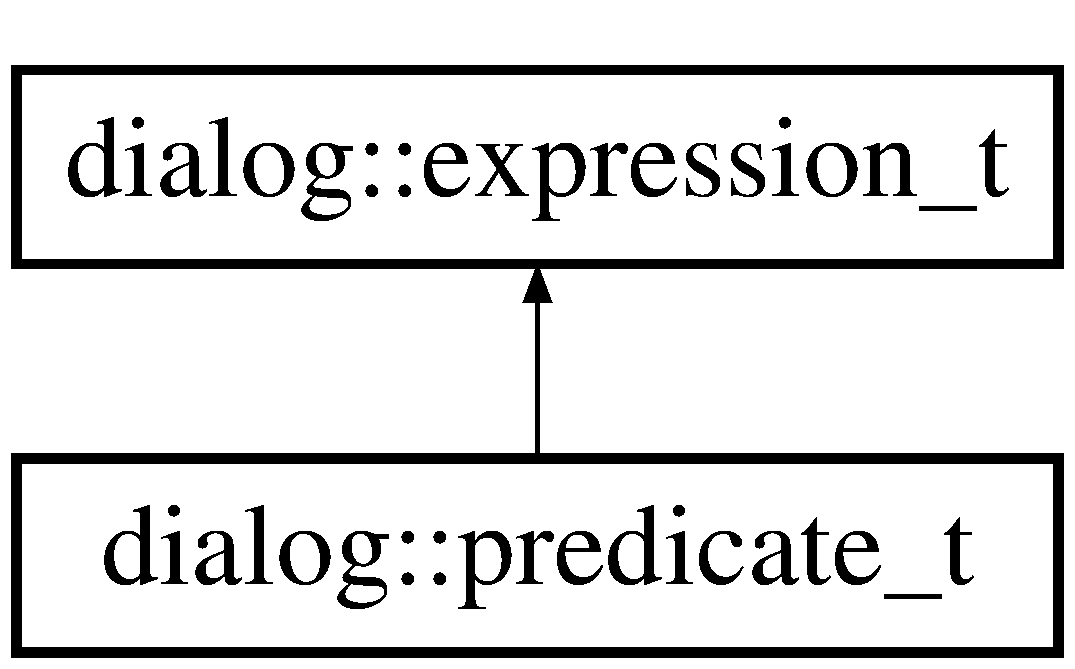
\includegraphics[height=2.000000cm]{structdialog_1_1predicate__t}
\end{center}
\end{figure}
\subsection*{Public Member Functions}
\begin{DoxyCompactItemize}
\item 
\mbox{\Hypertarget{structdialog_1_1predicate__t_af2595b51d4041f0a03fa3db46a0bbcb5}\label{structdialog_1_1predicate__t_af2595b51d4041f0a03fa3db46a0bbcb5}} 
{\bfseries predicate\+\_\+t} (const \hyperlink{structdialog_1_1predicate__t}{predicate\+\_\+t} \&other)
\item 
\mbox{\Hypertarget{structdialog_1_1predicate__t_a8fe17834ae8767c8aceebd8a4f5a92ac}\label{structdialog_1_1predicate__t_a8fe17834ae8767c8aceebd8a4f5a92ac}} 
\hyperlink{structdialog_1_1predicate__t}{predicate\+\_\+t} \& {\bfseries operator=} (const \hyperlink{structdialog_1_1predicate__t}{predicate\+\_\+t} \&other)
\item 
\mbox{\Hypertarget{structdialog_1_1predicate__t_ae8f4dd0d17d5ba98b3e8cf20daf14769}\label{structdialog_1_1predicate__t_ae8f4dd0d17d5ba98b3e8cf20daf14769}} 
bool {\bfseries operator$<$} (const \hyperlink{structdialog_1_1predicate__t}{predicate\+\_\+t} \&right) const
\item 
\mbox{\Hypertarget{structdialog_1_1predicate__t_a20f7619369e0b3162a09940ef366a222}\label{structdialog_1_1predicate__t_a20f7619369e0b3162a09940ef366a222}} 
std\+::string {\bfseries to\+\_\+string} () const
\end{DoxyCompactItemize}
\subsection*{Public Attributes}
\begin{DoxyCompactItemize}
\item 
\mbox{\Hypertarget{structdialog_1_1predicate__t_ad196d850f4d5b21587eec65b7fcd4a86}\label{structdialog_1_1predicate__t_ad196d850f4d5b21587eec65b7fcd4a86}} 
std\+::string {\bfseries attr}
\item 
\mbox{\Hypertarget{structdialog_1_1predicate__t_a6c416dda4b31ab90d25f9cac399cc66b}\label{structdialog_1_1predicate__t_a6c416dda4b31ab90d25f9cac399cc66b}} 
relop\+\_\+id {\bfseries op}
\item 
\mbox{\Hypertarget{structdialog_1_1predicate__t_a683944377ed3216bfbc2c08da9410645}\label{structdialog_1_1predicate__t_a683944377ed3216bfbc2c08da9410645}} 
std\+::string {\bfseries value}
\end{DoxyCompactItemize}


\subsection{Detailed Description}
Predicate expression. 

The documentation for this struct was generated from the following file\+:\begin{DoxyCompactItemize}
\item 
/\+Users/neil/\+Documents/\+Berkeley/research/dialog/libdialog/dialog/expression.\+h\end{DoxyCompactItemize}

\hypertarget{classdialog_1_1query__plan}{}\section{dialog\+:\+:query\+\_\+plan Class Reference}
\label{classdialog_1_1query__plan}\index{dialog\+::query\+\_\+plan@{dialog\+::query\+\_\+plan}}
Inheritance diagram for dialog\+:\+:query\+\_\+plan\+:\begin{figure}[H]
\begin{center}
\leavevmode
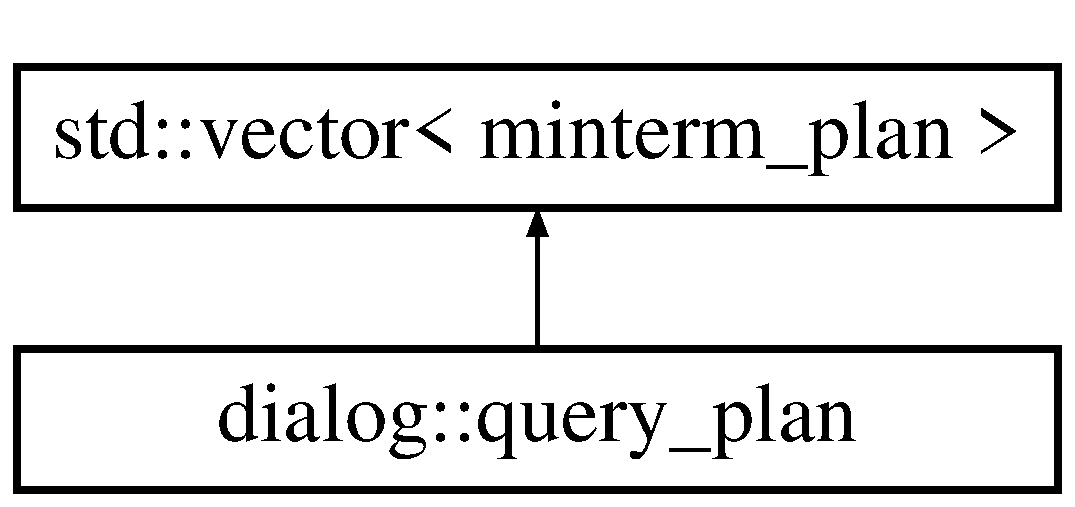
\includegraphics[height=2.000000cm]{classdialog_1_1query__plan}
\end{center}
\end{figure}
\subsection*{Public Member Functions}
\begin{DoxyCompactItemize}
\item 
\mbox{\Hypertarget{classdialog_1_1query__plan_ad7507d3597cd206396da2355e43a747f}\label{classdialog_1_1query__plan_ad7507d3597cd206396da2355e43a747f}} 
std\+::string {\bfseries to\+\_\+string} ()
\end{DoxyCompactItemize}


The documentation for this class was generated from the following file\+:\begin{DoxyCompactItemize}
\item 
/\+Users/neil/\+Documents/\+Berkeley/research/dialog/libdialog/dialog/query\+\_\+plan.\+h\end{DoxyCompactItemize}

\hypertarget{classdialog_1_1query__planner}{}\section{dialog\+:\+:query\+\_\+planner Class Reference}
\label{classdialog_1_1query__planner}\index{dialog\+::query\+\_\+planner@{dialog\+::query\+\_\+planner}}
\subsection*{Public Types}
\begin{DoxyCompactItemize}
\item 
\mbox{\Hypertarget{classdialog_1_1query__planner_a7510b75739e2eb9ec585a8e10ec2bfd4}\label{classdialog_1_1query__planner_a7510b75739e2eb9ec585a8e10ec2bfd4}} 
typedef std\+::vector$<$ \hyperlink{classdialog_1_1index__filter}{index\+\_\+filter} $>$ {\bfseries index\+\_\+filters}
\item 
\mbox{\Hypertarget{classdialog_1_1query__planner_a4779af06f1795c3c64823f9c8e81e155}\label{classdialog_1_1query__planner_a4779af06f1795c3c64823f9c8e81e155}} 
typedef index\+\_\+filters\+::iterator {\bfseries if\+\_\+iterator}
\item 
\mbox{\Hypertarget{classdialog_1_1query__planner_a0a361c6b6f817372b7e703b3fb0d4825}\label{classdialog_1_1query__planner_a0a361c6b6f817372b7e703b3fb0d4825}} 
typedef index\+\_\+filters\+::const\+\_\+iterator {\bfseries const\+\_\+if\+\_\+iterator}
\end{DoxyCompactItemize}
\subsection*{Public Member Functions}
\begin{DoxyCompactItemize}
\item 
\mbox{\Hypertarget{classdialog_1_1query__planner_a2769482e5e6a5e272f4801c6a88896b9}\label{classdialog_1_1query__planner_a2769482e5e6a5e272f4801c6a88896b9}} 
{\bfseries query\+\_\+planner} (const \hyperlink{structdialog_1_1compiled__expression}{compiled\+\_\+expression} \&expr, const \hyperlink{classdialog_1_1monolog_1_1monolog__exp2__linear}{index\+\_\+log} \&idx\+\_\+list)
\item 
\mbox{\Hypertarget{classdialog_1_1query__planner_af2a2e9a97346ac18038033b9083368e3}\label{classdialog_1_1query__planner_af2a2e9a97346ac18038033b9083368e3}} 
\hyperlink{classdialog_1_1query__plan}{query\+\_\+plan} {\bfseries plan} ()
\end{DoxyCompactItemize}


The documentation for this class was generated from the following file\+:\begin{DoxyCompactItemize}
\item 
/\+Users/neil/\+Documents/\+Berkeley/research/dialog/libdialog/dialog/query\+\_\+planner.\+h\end{DoxyCompactItemize}

\hypertarget{classdialog_1_1index_1_1radix__tree}{}\section{dialog\+:\+:index\+:\+:radix\+\_\+tree$<$ reflog $>$ Class Template Reference}
\label{classdialog_1_1index_1_1radix__tree}\index{dialog\+::index\+::radix\+\_\+tree$<$ reflog $>$@{dialog\+::index\+::radix\+\_\+tree$<$ reflog $>$}}
\subsection*{Public Types}
\begin{DoxyCompactItemize}
\item 
\mbox{\Hypertarget{classdialog_1_1index_1_1radix__tree_a4171083d914974526d788401cff4a769}\label{classdialog_1_1index_1_1radix__tree_a4171083d914974526d788401cff4a769}} 
typedef \hyperlink{structdialog_1_1index_1_1radix__tree__node}{radix\+\_\+tree\+\_\+node}$<$ \hyperlink{classdialog_1_1monolog_1_1monolog__exp2__linear}{reflog} $>$ {\bfseries node\+\_\+t}
\item 
\mbox{\Hypertarget{classdialog_1_1index_1_1radix__tree_a94d7e05cbfb067ca81642a059e45a868}\label{classdialog_1_1index_1_1radix__tree_a94d7e05cbfb067ca81642a059e45a868}} 
typedef \hyperlink{classdialog_1_1byte__string}{byte\+\_\+string} {\bfseries key\+\_\+t}
\item 
\mbox{\Hypertarget{classdialog_1_1index_1_1radix__tree_a860158d542bb505c99068fff580e4a68}\label{classdialog_1_1index_1_1radix__tree_a860158d542bb505c99068fff580e4a68}} 
typedef reflog\+::value\+\_\+type {\bfseries value\+\_\+t}
\item 
\mbox{\Hypertarget{classdialog_1_1index_1_1radix__tree_a7d6bb45239ec553be699b648fd66b3a3}\label{classdialog_1_1index_1_1radix__tree_a7d6bb45239ec553be699b648fd66b3a3}} 
typedef \hyperlink{classdialog_1_1index_1_1rt__reflog__it}{rt\+\_\+reflog\+\_\+it}$<$ \hyperlink{classdialog_1_1monolog_1_1monolog__exp2__linear}{reflog} $>$ {\bfseries iterator}
\item 
\mbox{\Hypertarget{classdialog_1_1index_1_1radix__tree_a993d828a62dd13f42e4a324ab90d934e}\label{classdialog_1_1index_1_1radix__tree_a993d828a62dd13f42e4a324ab90d934e}} 
typedef \hyperlink{classdialog_1_1index_1_1rt__reflog__range__result}{rt\+\_\+reflog\+\_\+range\+\_\+result}$<$ \hyperlink{classdialog_1_1monolog_1_1monolog__exp2__linear}{reflog} $>$ {\bfseries rt\+\_\+reflog\+\_\+result}
\item 
\mbox{\Hypertarget{classdialog_1_1index_1_1radix__tree_aa1adef4fed992b3ded3831a7180322d8}\label{classdialog_1_1index_1_1radix__tree_aa1adef4fed992b3ded3831a7180322d8}} 
typedef \hyperlink{classflattened__container}{flattened\+\_\+container}$<$ \hyperlink{classdialog_1_1index_1_1rt__reflog__range__result}{rt\+\_\+reflog\+\_\+range\+\_\+result}$<$ \hyperlink{classdialog_1_1monolog_1_1monolog__exp2__linear}{reflog} $>$ $>$ {\bfseries rt\+\_\+result}
\item 
\mbox{\Hypertarget{classdialog_1_1index_1_1radix__tree_adf3672f978967deefb01aa7c3b06bc6e}\label{classdialog_1_1index_1_1radix__tree_adf3672f978967deefb01aa7c3b06bc6e}} 
typedef \hyperlink{classflattened__iterator}{rt\+\_\+result\+::iterator} {\bfseries range\+\_\+iterator}
\end{DoxyCompactItemize}
\subsection*{Public Member Functions}
\begin{DoxyCompactItemize}
\item 
\mbox{\Hypertarget{classdialog_1_1index_1_1radix__tree_a346ba110c09cc087d49659d806425d7a}\label{classdialog_1_1index_1_1radix__tree_a346ba110c09cc087d49659d806425d7a}} 
{\bfseries radix\+\_\+tree} (size\+\_\+t depth, size\+\_\+t width)
\item 
\mbox{\Hypertarget{classdialog_1_1index_1_1radix__tree_ae219a6d4008450de31bc4784802fd84c}\label{classdialog_1_1index_1_1radix__tree_ae219a6d4008450de31bc4784802fd84c}} 
size\+\_\+t {\bfseries width} () const
\item 
\mbox{\Hypertarget{classdialog_1_1index_1_1radix__tree_aada7501fdd88e18f99e04a3a35e4038b}\label{classdialog_1_1index_1_1radix__tree_aada7501fdd88e18f99e04a3a35e4038b}} 
size\+\_\+t {\bfseries depth} () const
\item 
\mbox{\Hypertarget{classdialog_1_1index_1_1radix__tree_ad2e65fc7487e741e1339f4c7402348a6}\label{classdialog_1_1index_1_1radix__tree_ad2e65fc7487e741e1339f4c7402348a6}} 
{\footnotesize template$<$typename ... A\+R\+GS$>$ }\\\hyperlink{classdialog_1_1monolog_1_1monolog__exp2__linear}{reflog} $\ast$\& {\bfseries get\+\_\+or\+\_\+create} (const \hyperlink{classdialog_1_1byte__string}{key\+\_\+t} \&key, A\+R\+GS \&\&... args)
\item 
\mbox{\Hypertarget{classdialog_1_1index_1_1radix__tree_a07ff353f8a9eba5d557d8373f74fdb47}\label{classdialog_1_1index_1_1radix__tree_a07ff353f8a9eba5d557d8373f74fdb47}} 
{\footnotesize template$<$typename ... A\+R\+GS$>$ }\\\hyperlink{classdialog_1_1monolog_1_1monolog__exp2__linear}{reflog} $\ast$\& {\bfseries insert} (const \hyperlink{classdialog_1_1byte__string}{key\+\_\+t} \&key, const value\+\_\+t \&value, A\+R\+GS \&\&... args)
\item 
\mbox{\Hypertarget{classdialog_1_1index_1_1radix__tree_a2d637ae6eea61e95584234fb9a44db94}\label{classdialog_1_1index_1_1radix__tree_a2d637ae6eea61e95584234fb9a44db94}} 
\hyperlink{classdialog_1_1monolog_1_1monolog__exp2__linear}{reflog} const  $\ast$ {\bfseries get} (const \hyperlink{classdialog_1_1byte__string}{key\+\_\+t} \&key) const
\item 
\mbox{\Hypertarget{classdialog_1_1index_1_1radix__tree_ac6ca64025f76405f306fc7aa90074481}\label{classdialog_1_1index_1_1radix__tree_ac6ca64025f76405f306fc7aa90074481}} 
\hyperlink{classdialog_1_1monolog_1_1monolog__exp2__linear}{reflog} $\ast$ {\bfseries operator\mbox{[}$\,$\mbox{]}} (const \hyperlink{classdialog_1_1byte__string}{key\+\_\+t} \&key)
\item 
\mbox{\Hypertarget{classdialog_1_1index_1_1radix__tree_a19e7ca79ca0a850b8285cc298e6f13f0}\label{classdialog_1_1index_1_1radix__tree_a19e7ca79ca0a850b8285cc298e6f13f0}} 
\hyperlink{classdialog_1_1index_1_1rt__reflog__it}{iterator} {\bfseries upper\+\_\+bound} (const \hyperlink{classdialog_1_1byte__string}{key\+\_\+t} \&key) const
\item 
\mbox{\Hypertarget{classdialog_1_1index_1_1radix__tree_ab7abcb24a75757d0986ef4950008bdda}\label{classdialog_1_1index_1_1radix__tree_ab7abcb24a75757d0986ef4950008bdda}} 
\hyperlink{classdialog_1_1index_1_1rt__reflog__it}{iterator} {\bfseries lower\+\_\+bound} (const \hyperlink{classdialog_1_1byte__string}{key\+\_\+t} \&key) const
\item 
\mbox{\Hypertarget{classdialog_1_1index_1_1radix__tree_a70678f369aede02f2585c76720197916}\label{classdialog_1_1index_1_1radix__tree_a70678f369aede02f2585c76720197916}} 
\hyperlink{classdialog_1_1index_1_1rt__reflog__range__result}{rt\+\_\+reflog\+\_\+result} {\bfseries range\+\_\+lookup\+\_\+reflogs} (const \hyperlink{classdialog_1_1byte__string}{key\+\_\+t} \&begin, const \hyperlink{classdialog_1_1byte__string}{key\+\_\+t} \&end) const
\item 
\mbox{\Hypertarget{classdialog_1_1index_1_1radix__tree_a914163136bf6c3330c922855b93955f2}\label{classdialog_1_1index_1_1radix__tree_a914163136bf6c3330c922855b93955f2}} 
\hyperlink{classflattened__container}{rt\+\_\+result} {\bfseries range\+\_\+lookup} (const \hyperlink{classdialog_1_1byte__string}{key\+\_\+t} \&begin, const \hyperlink{classdialog_1_1byte__string}{key\+\_\+t} \&end) const
\item 
\mbox{\Hypertarget{classdialog_1_1index_1_1radix__tree_ab5f77a03120aed99761c005677bcda04}\label{classdialog_1_1index_1_1radix__tree_ab5f77a03120aed99761c005677bcda04}} 
size\+\_\+t {\bfseries approx\+\_\+count} (const \hyperlink{classdialog_1_1byte__string}{key\+\_\+t} \&begin, const \hyperlink{classdialog_1_1byte__string}{key\+\_\+t} \&end)
\end{DoxyCompactItemize}


The documentation for this class was generated from the following file\+:\begin{DoxyCompactItemize}
\item 
/\+Users/neil/\+Documents/\+Berkeley/research/dialog/libdialog/dialog/radix\+\_\+tree.\+h\end{DoxyCompactItemize}

\hypertarget{structdialog_1_1index_1_1radix__tree__node}{}\section{dialog\+:\+:index\+:\+:radix\+\_\+tree\+\_\+node$<$ reflog $>$ Struct Template Reference}
\label{structdialog_1_1index_1_1radix__tree__node}\index{dialog\+::index\+::radix\+\_\+tree\+\_\+node$<$ reflog $>$@{dialog\+::index\+::radix\+\_\+tree\+\_\+node$<$ reflog $>$}}
\subsection*{Public Types}
\begin{DoxyCompactItemize}
\item 
\mbox{\Hypertarget{structdialog_1_1index_1_1radix__tree__node_a0662b2a654d2ec8e56fe3dfe2c76f91d}\label{structdialog_1_1index_1_1radix__tree__node_a0662b2a654d2ec8e56fe3dfe2c76f91d}} 
typedef \hyperlink{structdialog_1_1index_1_1radix__tree__node}{radix\+\_\+tree\+\_\+node}$<$ \hyperlink{classdialog_1_1monolog_1_1monolog__exp2__linear}{reflog} $>$ {\bfseries node\+\_\+t}
\item 
\mbox{\Hypertarget{structdialog_1_1index_1_1radix__tree__node_a798fd98a8a69e6b92d5dad72639ba476}\label{structdialog_1_1index_1_1radix__tree__node_a798fd98a8a69e6b92d5dad72639ba476}} 
typedef atomic\+::type$<$ \hyperlink{structdialog_1_1index_1_1radix__tree__node}{node\+\_\+t} $\ast$ $>$ {\bfseries child\+\_\+t}
\item 
\mbox{\Hypertarget{structdialog_1_1index_1_1radix__tree__node_aa32bb8d1fe0da65e12965fc27dbcc9f3}\label{structdialog_1_1index_1_1radix__tree__node_aa32bb8d1fe0da65e12965fc27dbcc9f3}} 
typedef \hyperlink{classdialog_1_1byte__string}{byte\+\_\+string} {\bfseries key\+\_\+t}
\end{DoxyCompactItemize}
\subsection*{Public Member Functions}
\begin{DoxyCompactItemize}
\item 
\mbox{\Hypertarget{structdialog_1_1index_1_1radix__tree__node_afafdbd4fe0946b9813fd6e53144d12d7}\label{structdialog_1_1index_1_1radix__tree__node_afafdbd4fe0946b9813fd6e53144d12d7}} 
{\footnotesize template$<$typename ... A\+R\+GS$>$ }\\{\bfseries radix\+\_\+tree\+\_\+node} (uint8\+\_\+t node\+\_\+key, size\+\_\+t node\+\_\+width, size\+\_\+t node\+\_\+depth, \hyperlink{structdialog_1_1index_1_1radix__tree__node}{node\+\_\+t} $\ast$node\+\_\+parent, bool, A\+R\+GS \&\&... args)
\item 
\mbox{\Hypertarget{structdialog_1_1index_1_1radix__tree__node_a230cf563a8b4e2dac324791b7b30bcd4}\label{structdialog_1_1index_1_1radix__tree__node_a230cf563a8b4e2dac324791b7b30bcd4}} 
{\bfseries radix\+\_\+tree\+\_\+node} (uint8\+\_\+t node\+\_\+key, size\+\_\+t node\+\_\+width, size\+\_\+t node\+\_\+depth, \hyperlink{structdialog_1_1index_1_1radix__tree__node}{node\+\_\+t} $\ast$node\+\_\+parent)
\item 
\mbox{\Hypertarget{structdialog_1_1index_1_1radix__tree__node_a397829b9ff7017183deb7dcc2623d3d4}\label{structdialog_1_1index_1_1radix__tree__node_a397829b9ff7017183deb7dcc2623d3d4}} 
\hyperlink{classdialog_1_1monolog_1_1monolog__exp2__linear}{reflog} $\ast$\& {\bfseries refs} ()
\item 
\mbox{\Hypertarget{structdialog_1_1index_1_1radix__tree__node_ac0c04b6f6d5357feca1ebfd345d13707}\label{structdialog_1_1index_1_1radix__tree__node_ac0c04b6f6d5357feca1ebfd345d13707}} 
\hyperlink{classdialog_1_1monolog_1_1monolog__exp2__linear}{reflog} $\ast$const  \& {\bfseries refs} () const
\item 
\mbox{\Hypertarget{structdialog_1_1index_1_1radix__tree__node_a2b99436aae6d96c0c4ceb612b4748a58}\label{structdialog_1_1index_1_1radix__tree__node_a2b99436aae6d96c0c4ceb612b4748a58}} 
child\+\_\+t $\ast$\& {\bfseries children} ()
\item 
\mbox{\Hypertarget{structdialog_1_1index_1_1radix__tree__node_a5a6c3fc732f518c2ed3ec080afc468ba}\label{structdialog_1_1index_1_1radix__tree__node_a5a6c3fc732f518c2ed3ec080afc468ba}} 
child\+\_\+t $\ast$const  \& {\bfseries children} () const
\item 
\mbox{\Hypertarget{structdialog_1_1index_1_1radix__tree__node_a0305272882f54699ce555c1c8e72d5ba}\label{structdialog_1_1index_1_1radix__tree__node_a0305272882f54699ce555c1c8e72d5ba}} 
const \hyperlink{structdialog_1_1index_1_1radix__tree__node}{node\+\_\+t} $\ast$ {\bfseries first\+\_\+child} (size\+\_\+t width) const
\item 
\mbox{\Hypertarget{structdialog_1_1index_1_1radix__tree__node_a35eb69ba2cb5a5300de64331619f3c5d}\label{structdialog_1_1index_1_1radix__tree__node_a35eb69ba2cb5a5300de64331619f3c5d}} 
const \hyperlink{structdialog_1_1index_1_1radix__tree__node}{node\+\_\+t} $\ast$ {\bfseries last\+\_\+child} (size\+\_\+t width) const
\item 
\mbox{\Hypertarget{structdialog_1_1index_1_1radix__tree__node_a59c5bae980c11d89d714630d440fd964}\label{structdialog_1_1index_1_1radix__tree__node_a59c5bae980c11d89d714630d440fd964}} 
const \hyperlink{structdialog_1_1index_1_1radix__tree__node}{node\+\_\+t} $\ast$ {\bfseries next\+\_\+child} (uint8\+\_\+t key, size\+\_\+t width) const
\item 
\mbox{\Hypertarget{structdialog_1_1index_1_1radix__tree__node_ae28a3dff60ac574327ef8812b26e9173}\label{structdialog_1_1index_1_1radix__tree__node_ae28a3dff60ac574327ef8812b26e9173}} 
const \hyperlink{structdialog_1_1index_1_1radix__tree__node}{node\+\_\+t} $\ast$ {\bfseries prev\+\_\+child} (uint8\+\_\+t key, size\+\_\+t width) const
\item 
\mbox{\Hypertarget{structdialog_1_1index_1_1radix__tree__node_a4f3f487295eacd60061d710104ade025}\label{structdialog_1_1index_1_1radix__tree__node_a4f3f487295eacd60061d710104ade025}} 
const \hyperlink{structdialog_1_1index_1_1radix__tree__node}{node\+\_\+t} $\ast$ {\bfseries advance} (\hyperlink{classdialog_1_1byte__string}{key\+\_\+t} \&t\+\_\+key, size\+\_\+t t\+\_\+width, size\+\_\+t t\+\_\+depth) const
\item 
\mbox{\Hypertarget{structdialog_1_1index_1_1radix__tree__node_aa781f4973238e053bfd131c28e8ff8e2}\label{structdialog_1_1index_1_1radix__tree__node_aa781f4973238e053bfd131c28e8ff8e2}} 
const \hyperlink{structdialog_1_1index_1_1radix__tree__node}{node\+\_\+t} $\ast$ {\bfseries advance\+\_\+descend} (\hyperlink{classdialog_1_1byte__string}{key\+\_\+t} \&t\+\_\+key, size\+\_\+t t\+\_\+width, size\+\_\+t t\+\_\+depth) const
\item 
\mbox{\Hypertarget{structdialog_1_1index_1_1radix__tree__node_a74ab89b8f9791631b5457aba7d9a37d4}\label{structdialog_1_1index_1_1radix__tree__node_a74ab89b8f9791631b5457aba7d9a37d4}} 
const \hyperlink{structdialog_1_1index_1_1radix__tree__node}{node\+\_\+t} $\ast$ {\bfseries retreat} (\hyperlink{classdialog_1_1byte__string}{key\+\_\+t} \&t\+\_\+key, size\+\_\+t t\+\_\+width, size\+\_\+t t\+\_\+depth) const
\item 
\mbox{\Hypertarget{structdialog_1_1index_1_1radix__tree__node_a18804efbeade1df1028f2ccdada36a27}\label{structdialog_1_1index_1_1radix__tree__node_a18804efbeade1df1028f2ccdada36a27}} 
const \hyperlink{structdialog_1_1index_1_1radix__tree__node}{node\+\_\+t} $\ast$ {\bfseries retreat\+\_\+descend} (\hyperlink{classdialog_1_1byte__string}{key\+\_\+t} \&t\+\_\+key, size\+\_\+t t\+\_\+width, size\+\_\+t t\+\_\+depth) const
\end{DoxyCompactItemize}
\subsection*{Public Attributes}
\begin{DoxyCompactItemize}
\item 
\mbox{\Hypertarget{structdialog_1_1index_1_1radix__tree__node_ae671cbfb97860434cfa1b1508807da6c}\label{structdialog_1_1index_1_1radix__tree__node_ae671cbfb97860434cfa1b1508807da6c}} 
uint8\+\_\+t {\bfseries key}
\item 
\mbox{\Hypertarget{structdialog_1_1index_1_1radix__tree__node_ac8057cfc7492d204d6997ce4b5151846}\label{structdialog_1_1index_1_1radix__tree__node_ac8057cfc7492d204d6997ce4b5151846}} 
uint8\+\_\+t {\bfseries depth}
\item 
\mbox{\Hypertarget{structdialog_1_1index_1_1radix__tree__node_adee6d7afc7e021b9f432e1766c908594}\label{structdialog_1_1index_1_1radix__tree__node_adee6d7afc7e021b9f432e1766c908594}} 
void $\ast$ {\bfseries data}
\item 
\mbox{\Hypertarget{structdialog_1_1index_1_1radix__tree__node_a149dbbb1e15ebc571ece3e6aeafa3392}\label{structdialog_1_1index_1_1radix__tree__node_a149dbbb1e15ebc571ece3e6aeafa3392}} 
bool {\bfseries is\+\_\+leaf}
\item 
\mbox{\Hypertarget{structdialog_1_1index_1_1radix__tree__node_ace7536851ade6aa80f8aeafcf9a6ec39}\label{structdialog_1_1index_1_1radix__tree__node_ace7536851ade6aa80f8aeafcf9a6ec39}} 
\hyperlink{structdialog_1_1index_1_1radix__tree__node}{node\+\_\+t} $\ast$ {\bfseries parent}
\end{DoxyCompactItemize}


The documentation for this struct was generated from the following file\+:\begin{DoxyCompactItemize}
\item 
/\+Users/neil/\+Documents/\+Berkeley/research/dialog/libdialog/dialog/radix\+\_\+tree.\+h\end{DoxyCompactItemize}

\hypertarget{classdialog_1_1read__tail}{}\section{dialog\+:\+:read\+\_\+tail Class Reference}
\label{classdialog_1_1read__tail}\index{dialog\+::read\+\_\+tail@{dialog\+::read\+\_\+tail}}
\subsection*{Public Member Functions}
\begin{DoxyCompactItemize}
\item 
\mbox{\Hypertarget{classdialog_1_1read__tail_a2c33565f837dad30ceb0ca773eaf4332}\label{classdialog_1_1read__tail_a2c33565f837dad30ceb0ca773eaf4332}} 
{\bfseries read\+\_\+tail} (const std\+::string \&data\+\_\+path, const \hyperlink{structdialog_1_1storage_1_1storage__mode}{storage\+::storage\+\_\+mode} \&storage)
\item 
\mbox{\Hypertarget{classdialog_1_1read__tail_a61857cc04e420a980da27f07f86fb8bb}\label{classdialog_1_1read__tail_a61857cc04e420a980da27f07f86fb8bb}} 
void {\bfseries init} (const std\+::string \&data\+\_\+path, const \hyperlink{structdialog_1_1storage_1_1storage__mode}{storage\+::storage\+\_\+mode} \&storage)
\item 
\mbox{\Hypertarget{classdialog_1_1read__tail_ae0ee05a10b3765b5df2be3321edee939}\label{classdialog_1_1read__tail_ae0ee05a10b3765b5df2be3321edee939}} 
uint64\+\_\+t {\bfseries get} () const
\item 
\mbox{\Hypertarget{classdialog_1_1read__tail_a542d09c03134765b8a33665d9a01e23f}\label{classdialog_1_1read__tail_a542d09c03134765b8a33665d9a01e23f}} 
void {\bfseries advance} (uint64\+\_\+t old\+\_\+tail, uint32\+\_\+t bytes)
\end{DoxyCompactItemize}


The documentation for this class was generated from the following file\+:\begin{DoxyCompactItemize}
\item 
/\+Users/neil/\+Documents/\+Berkeley/research/dialog/libdialog/dialog/read\+\_\+tail.\+h\end{DoxyCompactItemize}

\hypertarget{structdialog_1_1record__batch}{}\section{dialog\+:\+:record\+\_\+batch Struct Reference}
\label{structdialog_1_1record__batch}\index{dialog\+::record\+\_\+batch@{dialog\+::record\+\_\+batch}}
\subsection*{Public Member Functions}
\begin{DoxyCompactItemize}
\item 
\mbox{\Hypertarget{structdialog_1_1record__batch_a888a26ec19e97a8c95f1d63389b42347}\label{structdialog_1_1record__batch_a888a26ec19e97a8c95f1d63389b42347}} 
int64\+\_\+t {\bfseries start\+\_\+time\+\_\+block} () const
\item 
\mbox{\Hypertarget{structdialog_1_1record__batch_a0b93d4224a917916a1df16f9ccad91fd}\label{structdialog_1_1record__batch_a0b93d4224a917916a1df16f9ccad91fd}} 
int64\+\_\+t {\bfseries end\+\_\+time\+\_\+block} () const
\end{DoxyCompactItemize}
\subsection*{Public Attributes}
\begin{DoxyCompactItemize}
\item 
\mbox{\Hypertarget{structdialog_1_1record__batch_ae67753e518bfa1d6dc617f9a922c6052}\label{structdialog_1_1record__batch_ae67753e518bfa1d6dc617f9a922c6052}} 
std\+::vector$<$ \hyperlink{structdialog_1_1record__block}{record\+\_\+block} $>$ {\bfseries blocks}
\item 
\mbox{\Hypertarget{structdialog_1_1record__batch_a8aa53a8f0e28820860364f31775cc7a8}\label{structdialog_1_1record__batch_a8aa53a8f0e28820860364f31775cc7a8}} 
size\+\_\+t {\bfseries nrecords}
\end{DoxyCompactItemize}


The documentation for this struct was generated from the following file\+:\begin{DoxyCompactItemize}
\item 
/\+Users/neil/\+Documents/\+Berkeley/research/dialog/libdialog/dialog/record\+\_\+batch.\+h\end{DoxyCompactItemize}

\hypertarget{classdialog_1_1record__batch__builder}{}\section{dialog\+:\+:record\+\_\+batch\+\_\+builder Class Reference}
\label{classdialog_1_1record__batch__builder}\index{dialog\+::record\+\_\+batch\+\_\+builder@{dialog\+::record\+\_\+batch\+\_\+builder}}
\subsection*{Public Member Functions}
\begin{DoxyCompactItemize}
\item 
\mbox{\Hypertarget{classdialog_1_1record__batch__builder_a186db23833312d999558edb7ee8c2c0c}\label{classdialog_1_1record__batch__builder_a186db23833312d999558edb7ee8c2c0c}} 
void {\bfseries add\+\_\+record} (const std\+::string \&rec)
\item 
\mbox{\Hypertarget{classdialog_1_1record__batch__builder_af17f5ac86d5183adda6ba1f77f8b0460}\label{classdialog_1_1record__batch__builder_af17f5ac86d5183adda6ba1f77f8b0460}} 
void {\bfseries add\+\_\+record} (std\+::string \&\&rec)
\item 
\mbox{\Hypertarget{classdialog_1_1record__batch__builder_a8c74ad06d5011ec0c27b759fc860b305}\label{classdialog_1_1record__batch__builder_a8c74ad06d5011ec0c27b759fc860b305}} 
\hyperlink{structdialog_1_1record__batch}{record\+\_\+batch} {\bfseries get\+\_\+batch} ()
\end{DoxyCompactItemize}
\subsection*{Static Public Attributes}
\begin{DoxyCompactItemize}
\item 
\mbox{\Hypertarget{classdialog_1_1record__batch__builder_a147e4a0f71ba1253cb559abe2b70286d}\label{classdialog_1_1record__batch__builder_a147e4a0f71ba1253cb559abe2b70286d}} 
static const int64\+\_\+t {\bfseries T\+I\+M\+E\+\_\+\+B\+L\+O\+CK} = 1e6
\end{DoxyCompactItemize}


The documentation for this class was generated from the following file\+:\begin{DoxyCompactItemize}
\item 
/\+Users/neil/\+Documents/\+Berkeley/research/dialog/libdialog/dialog/record\+\_\+batch.\+h\end{DoxyCompactItemize}

\hypertarget{structdialog_1_1record__block}{}\section{dialog\+:\+:record\+\_\+block Struct Reference}
\label{structdialog_1_1record__block}\index{dialog\+::record\+\_\+block@{dialog\+::record\+\_\+block}}
\subsection*{Public Attributes}
\begin{DoxyCompactItemize}
\item 
\mbox{\Hypertarget{structdialog_1_1record__block_a455e5d4b183709b019249312e6962df7}\label{structdialog_1_1record__block_a455e5d4b183709b019249312e6962df7}} 
int64\+\_\+t {\bfseries time\+\_\+block}
\item 
\mbox{\Hypertarget{structdialog_1_1record__block_a8e9d9fadaf0ef3fc55a26f3e439d4db1}\label{structdialog_1_1record__block_a8e9d9fadaf0ef3fc55a26f3e439d4db1}} 
std\+::string {\bfseries data}
\item 
\mbox{\Hypertarget{structdialog_1_1record__block_a9496f8995310f46fd976d56995d2a0f7}\label{structdialog_1_1record__block_a9496f8995310f46fd976d56995d2a0f7}} 
size\+\_\+t {\bfseries nrecords}
\end{DoxyCompactItemize}


The documentation for this struct was generated from the following file\+:\begin{DoxyCompactItemize}
\item 
/\+Users/neil/\+Documents/\+Berkeley/research/dialog/libdialog/dialog/record\+\_\+batch.\+h\end{DoxyCompactItemize}

\hypertarget{classdialog_1_1record__stream}{}\section{dialog\+:\+:record\+\_\+stream$<$ offset\+\_\+container $>$ Class Template Reference}
\label{classdialog_1_1record__stream}\index{dialog\+::record\+\_\+stream$<$ offset\+\_\+container $>$@{dialog\+::record\+\_\+stream$<$ offset\+\_\+container $>$}}
\subsection*{Public Types}
\begin{DoxyCompactItemize}
\item 
\mbox{\Hypertarget{classdialog_1_1record__stream_ad2e87f19c47fed1ab24f95c374621d55}\label{classdialog_1_1record__stream_ad2e87f19c47fed1ab24f95c374621d55}} 
typedef std\+::forward\+\_\+iterator\+\_\+tag {\bfseries iterator\+\_\+category}
\item 
\mbox{\Hypertarget{classdialog_1_1record__stream_a42dbf21e91ba40e6532a95d7015be1eb}\label{classdialog_1_1record__stream_a42dbf21e91ba40e6532a95d7015be1eb}} 
typedef \hyperlink{structdialog_1_1record__t}{record\+\_\+t} {\bfseries value\+\_\+type}
\item 
\mbox{\Hypertarget{classdialog_1_1record__stream_af5467b1ca78962cebe23ea9c78a5d32d}\label{classdialog_1_1record__stream_af5467b1ca78962cebe23ea9c78a5d32d}} 
typedef offset\+\_\+container\+::iterator {\bfseries offset\+\_\+iterator}
\end{DoxyCompactItemize}
\subsection*{Public Member Functions}
\begin{DoxyCompactItemize}
\item 
\mbox{\Hypertarget{classdialog_1_1record__stream_a42921aa2b1009eed0c94e4abde6bf11f}\label{classdialog_1_1record__stream_a42921aa2b1009eed0c94e4abde6bf11f}} 
{\bfseries record\+\_\+stream} (uint64\+\_\+t version, const offset\+\_\+container \&offsets, const \hyperlink{classdialog_1_1schema__t}{schema\+\_\+t} \&schema, const \hyperlink{classdialog_1_1monolog_1_1monolog__linear}{data\+\_\+log} \&\hyperlink{classdialog_1_1monolog_1_1monolog__linear}{data\+\_\+log})
\item 
\mbox{\Hypertarget{classdialog_1_1record__stream_a763e108fd83b5371e0abd425cbac1554}\label{classdialog_1_1record__stream_a763e108fd83b5371e0abd425cbac1554}} 
\hyperlink{structdialog_1_1record__t}{record\+\_\+t} {\bfseries get} () const
\item 
\mbox{\Hypertarget{classdialog_1_1record__stream_a809d836d1e0355a80585110449cf28ba}\label{classdialog_1_1record__stream_a809d836d1e0355a80585110449cf28ba}} 
\hyperlink{classdialog_1_1record__stream}{record\+\_\+stream} \& {\bfseries operator++} ()
\item 
\mbox{\Hypertarget{classdialog_1_1record__stream_a1dad40319a37342cdb1be4dab9d7507d}\label{classdialog_1_1record__stream_a1dad40319a37342cdb1be4dab9d7507d}} 
\hyperlink{classdialog_1_1record__stream}{record\+\_\+stream} \& {\bfseries operator++} (int)
\item 
\mbox{\Hypertarget{classdialog_1_1record__stream_a5c4e497673511f6744dbadd96e2377fe}\label{classdialog_1_1record__stream_a5c4e497673511f6744dbadd96e2377fe}} 
bool {\bfseries has\+\_\+more} () const
\end{DoxyCompactItemize}
\subsection*{Friends}
\begin{DoxyCompactItemize}
\item 
\mbox{\Hypertarget{classdialog_1_1record__stream_ad7a7dec15a4ce64b94d09539f25e5a39}\label{classdialog_1_1record__stream_ad7a7dec15a4ce64b94d09539f25e5a39}} 
bool {\bfseries operator==} (const \hyperlink{classdialog_1_1record__stream}{record\+\_\+stream} \&a, const \hyperlink{classdialog_1_1record__stream}{record\+\_\+stream} \&b)
\item 
\mbox{\Hypertarget{classdialog_1_1record__stream_ade8067f06c184a05dd323e726033f4a8}\label{classdialog_1_1record__stream_ade8067f06c184a05dd323e726033f4a8}} 
bool {\bfseries operator!=} (const \hyperlink{classdialog_1_1record__stream}{record\+\_\+stream} \&a, const \hyperlink{classdialog_1_1record__stream}{record\+\_\+stream} \&b)
\end{DoxyCompactItemize}


The documentation for this class was generated from the following file\+:\begin{DoxyCompactItemize}
\item 
/\+Users/neil/\+Documents/\+Berkeley/research/dialog/libdialog/dialog/record\+\_\+stream.\+h\end{DoxyCompactItemize}

\hypertarget{structdialog_1_1record__t}{}\section{dialog\+:\+:record\+\_\+t Struct Reference}
\label{structdialog_1_1record__t}\index{dialog\+::record\+\_\+t@{dialog\+::record\+\_\+t}}
\subsection*{Public Types}
\begin{DoxyCompactItemize}
\item 
\mbox{\Hypertarget{structdialog_1_1record__t_af4e986b15f9ca35c54a4ab6e8c52d30f}\label{structdialog_1_1record__t_af4e986b15f9ca35c54a4ab6e8c52d30f}} 
typedef std\+::vector$<$ \hyperlink{structdialog_1_1field__t}{field\+\_\+t} $>$\+::iterator {\bfseries iterator}
\item 
\mbox{\Hypertarget{structdialog_1_1record__t_a7e34b0f2b52763beee231a58e3263c17}\label{structdialog_1_1record__t_a7e34b0f2b52763beee231a58e3263c17}} 
typedef std\+::vector$<$ \hyperlink{structdialog_1_1field__t}{field\+\_\+t} $>$\+::const\+\_\+iterator {\bfseries const\+\_\+iterator}
\end{DoxyCompactItemize}
\subsection*{Public Member Functions}
\begin{DoxyCompactItemize}
\item 
\mbox{\Hypertarget{structdialog_1_1record__t_a3e010a7750deea6edd3ea9b7c557c900}\label{structdialog_1_1record__t_a3e010a7750deea6edd3ea9b7c557c900}} 
{\bfseries record\+\_\+t} (size\+\_\+t log\+\_\+offset, void $\ast$\hyperlink{structdialog_1_1data}{data}, size\+\_\+t size)
\item 
\mbox{\Hypertarget{structdialog_1_1record__t_a003ed255f19d457f16ca593f841912e0}\label{structdialog_1_1record__t_a003ed255f19d457f16ca593f841912e0}} 
void {\bfseries reserve} (size\+\_\+t n)
\item 
\mbox{\Hypertarget{structdialog_1_1record__t_aa52eed245247cc9546c8f54a1bb79626}\label{structdialog_1_1record__t_aa52eed245247cc9546c8f54a1bb79626}} 
void {\bfseries push\+\_\+back} (const \hyperlink{structdialog_1_1field__t}{field\+\_\+t} \&val)
\item 
\mbox{\Hypertarget{structdialog_1_1record__t_a6e1501e143bccb395442eaedd6d2352a}\label{structdialog_1_1record__t_a6e1501e143bccb395442eaedd6d2352a}} 
void {\bfseries push\+\_\+back} (\hyperlink{structdialog_1_1field__t}{field\+\_\+t} \&\&val)
\item 
\mbox{\Hypertarget{structdialog_1_1record__t_a0c2bf230c9156eaba00a3ceabfcb95d7}\label{structdialog_1_1record__t_a0c2bf230c9156eaba00a3ceabfcb95d7}} 
const \hyperlink{structdialog_1_1field__t}{field\+\_\+t} \& {\bfseries operator\mbox{[}$\,$\mbox{]}} (uint16\+\_\+t idx) const
\item 
\mbox{\Hypertarget{structdialog_1_1record__t_a11abc485ed657db030ddbe441e1d45d3}\label{structdialog_1_1record__t_a11abc485ed657db030ddbe441e1d45d3}} 
const \hyperlink{structdialog_1_1field__t}{field\+\_\+t} \& {\bfseries at} (uint16\+\_\+t idx) const
\item 
\mbox{\Hypertarget{structdialog_1_1record__t_aa3a7c889e5f3013df010cad5217d5e11}\label{structdialog_1_1record__t_aa3a7c889e5f3013df010cad5217d5e11}} 
uint64\+\_\+t {\bfseries timestamp} () const
\item 
\mbox{\Hypertarget{structdialog_1_1record__t_a2bd7e9bf1821ff2d23b32910c3f34934}\label{structdialog_1_1record__t_a2bd7e9bf1821ff2d23b32910c3f34934}} 
size\+\_\+t {\bfseries log\+\_\+offset} () const
\item 
\mbox{\Hypertarget{structdialog_1_1record__t_a4bc3b102414bc572fdc07309ef0f0a7a}\label{structdialog_1_1record__t_a4bc3b102414bc572fdc07309ef0f0a7a}} 
void $\ast$ {\bfseries data} () const
\item 
\mbox{\Hypertarget{structdialog_1_1record__t_a52dbda4f5f04a5ec4c5588241c3a5533}\label{structdialog_1_1record__t_a52dbda4f5f04a5ec4c5588241c3a5533}} 
uint64\+\_\+t {\bfseries version} () const
\item 
\mbox{\Hypertarget{structdialog_1_1record__t_a841131722da9228e784e29188ba77c5b}\label{structdialog_1_1record__t_a841131722da9228e784e29188ba77c5b}} 
iterator {\bfseries begin} ()
\item 
\mbox{\Hypertarget{structdialog_1_1record__t_ae0881e9d5b98f01480cb62da5441795c}\label{structdialog_1_1record__t_ae0881e9d5b98f01480cb62da5441795c}} 
iterator {\bfseries end} ()
\item 
\mbox{\Hypertarget{structdialog_1_1record__t_a56205f6df46bbd0003d33c7a1fc97814}\label{structdialog_1_1record__t_a56205f6df46bbd0003d33c7a1fc97814}} 
const\+\_\+iterator {\bfseries begin} () const
\item 
\mbox{\Hypertarget{structdialog_1_1record__t_a3c11548c92f6fe3c8c02adaeeca3a6f1}\label{structdialog_1_1record__t_a3c11548c92f6fe3c8c02adaeeca3a6f1}} 
const\+\_\+iterator {\bfseries end} () const
\item 
\mbox{\Hypertarget{structdialog_1_1record__t_a6b7f1ea9625f0dad11bc53dcedb2f1a6}\label{structdialog_1_1record__t_a6b7f1ea9625f0dad11bc53dcedb2f1a6}} 
size\+\_\+t {\bfseries length} () const
\item 
\mbox{\Hypertarget{structdialog_1_1record__t_a60677227ea92a2e7672bd4bb16d615f3}\label{structdialog_1_1record__t_a60677227ea92a2e7672bd4bb16d615f3}} 
std\+::string {\bfseries to\+\_\+string} () const
\end{DoxyCompactItemize}


The documentation for this struct was generated from the following file\+:\begin{DoxyCompactItemize}
\item 
/\+Users/neil/\+Documents/\+Berkeley/research/dialog/libdialog/dialog/record.\+h\end{DoxyCompactItemize}

\hypertarget{classdialog_1_1relop__utils}{}\section{dialog\+:\+:relop\+\_\+utils Class Reference}
\label{classdialog_1_1relop__utils}\index{dialog\+::relop\+\_\+utils@{dialog\+::relop\+\_\+utils}}
\subsection*{Static Public Member Functions}
\begin{DoxyCompactItemize}
\item 
static relop\+\_\+id \hyperlink{classdialog_1_1relop__utils_a6dd36213f1e18ce3408281da2dae561c}{str\+\_\+to\+\_\+op} (const std\+::string \&op)
\item 
static std\+::string \hyperlink{classdialog_1_1relop__utils_aa2ece63f9eb4bc6e0af2aef09fcfc8e2}{op\+\_\+to\+\_\+str} (const relop\+\_\+id \&op)
\end{DoxyCompactItemize}


\subsection{Member Function Documentation}
\mbox{\Hypertarget{classdialog_1_1relop__utils_aa2ece63f9eb4bc6e0af2aef09fcfc8e2}\label{classdialog_1_1relop__utils_aa2ece63f9eb4bc6e0af2aef09fcfc8e2}} 
\index{dialog\+::relop\+\_\+utils@{dialog\+::relop\+\_\+utils}!op\+\_\+to\+\_\+str@{op\+\_\+to\+\_\+str}}
\index{op\+\_\+to\+\_\+str@{op\+\_\+to\+\_\+str}!dialog\+::relop\+\_\+utils@{dialog\+::relop\+\_\+utils}}
\subsubsection{\texorpdfstring{op\+\_\+to\+\_\+str()}{op\_to\_str()}}
{\footnotesize\ttfamily static std\+::string dialog\+::relop\+\_\+utils\+::op\+\_\+to\+\_\+str (\begin{DoxyParamCaption}\item[{const relop\+\_\+id \&}]{op }\end{DoxyParamCaption})\hspace{0.3cm}{\ttfamily [inline]}, {\ttfamily [static]}}

Converts a relop\+\_\+id enum to string


\begin{DoxyParams}{Parameters}
{\em op} & relop\+\_\+id enum \\
\hline
\end{DoxyParams}
\begin{DoxyReturn}{Returns}
String representation of operator 
\end{DoxyReturn}
\mbox{\Hypertarget{classdialog_1_1relop__utils_a6dd36213f1e18ce3408281da2dae561c}\label{classdialog_1_1relop__utils_a6dd36213f1e18ce3408281da2dae561c}} 
\index{dialog\+::relop\+\_\+utils@{dialog\+::relop\+\_\+utils}!str\+\_\+to\+\_\+op@{str\+\_\+to\+\_\+op}}
\index{str\+\_\+to\+\_\+op@{str\+\_\+to\+\_\+op}!dialog\+::relop\+\_\+utils@{dialog\+::relop\+\_\+utils}}
\subsubsection{\texorpdfstring{str\+\_\+to\+\_\+op()}{str\_to\_op()}}
{\footnotesize\ttfamily static relop\+\_\+id dialog\+::relop\+\_\+utils\+::str\+\_\+to\+\_\+op (\begin{DoxyParamCaption}\item[{const std\+::string \&}]{op }\end{DoxyParamCaption})\hspace{0.3cm}{\ttfamily [inline]}, {\ttfamily [static]}}

Converts a string operator to relop\+\_\+id enum


\begin{DoxyParams}{Parameters}
{\em op} & String operator \\
\hline
\end{DoxyParams}
\begin{DoxyReturn}{Returns}
relop\+\_\+id enum 
\end{DoxyReturn}


The documentation for this class was generated from the following file\+:\begin{DoxyCompactItemize}
\item 
/\+Users/neil/\+Documents/\+Berkeley/research/dialog/libdialog/dialog/relational\+\_\+ops.\+h\end{DoxyCompactItemize}

\hypertarget{classdialog_1_1index_1_1rt__reflog__it}{}\section{dialog\+:\+:index\+:\+:rt\+\_\+reflog\+\_\+it$<$ reflog $>$ Class Template Reference}
\label{classdialog_1_1index_1_1rt__reflog__it}\index{dialog\+::index\+::rt\+\_\+reflog\+\_\+it$<$ reflog $>$@{dialog\+::index\+::rt\+\_\+reflog\+\_\+it$<$ reflog $>$}}
Inheritance diagram for dialog\+:\+:index\+:\+:rt\+\_\+reflog\+\_\+it$<$ reflog $>$\+:\begin{figure}[H]
\begin{center}
\leavevmode
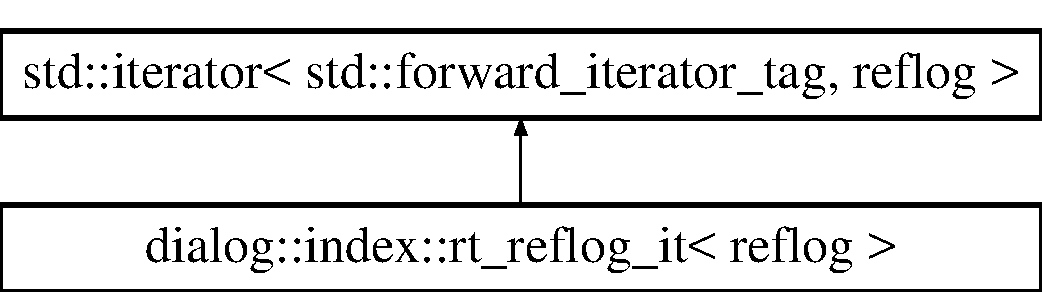
\includegraphics[height=2.000000cm]{classdialog_1_1index_1_1rt__reflog__it}
\end{center}
\end{figure}
\subsection*{Public Types}
\begin{DoxyCompactItemize}
\item 
\mbox{\Hypertarget{classdialog_1_1index_1_1rt__reflog__it_afe71079375b6d14c69582edc4c67620f}\label{classdialog_1_1index_1_1rt__reflog__it_afe71079375b6d14c69582edc4c67620f}} 
typedef \hyperlink{structdialog_1_1index_1_1radix__tree__node}{radix\+\_\+tree\+\_\+node}$<$ \hyperlink{classdialog_1_1monolog_1_1monolog__exp2__linear}{reflog} $>$ {\bfseries node\+\_\+t}
\item 
\mbox{\Hypertarget{classdialog_1_1index_1_1rt__reflog__it_aa870823322e7ac72f3282e663336356b}\label{classdialog_1_1index_1_1rt__reflog__it_aa870823322e7ac72f3282e663336356b}} 
typedef \hyperlink{classdialog_1_1byte__string}{byte\+\_\+string} {\bfseries key\+\_\+t}
\item 
\mbox{\Hypertarget{classdialog_1_1index_1_1rt__reflog__it_a684d45937aeedcc0deb4f0f357efb480}\label{classdialog_1_1index_1_1rt__reflog__it_a684d45937aeedcc0deb4f0f357efb480}} 
typedef \hyperlink{classdialog_1_1index_1_1rt__reflog__it}{rt\+\_\+reflog\+\_\+it}$<$ \hyperlink{classdialog_1_1monolog_1_1monolog__exp2__linear}{reflog} $>$ {\bfseries self\+\_\+type}
\item 
\mbox{\Hypertarget{classdialog_1_1index_1_1rt__reflog__it_aa7a279113eed81533102d13726d252f6}\label{classdialog_1_1index_1_1rt__reflog__it_aa7a279113eed81533102d13726d252f6}} 
typedef \hyperlink{classdialog_1_1monolog_1_1monolog__exp2__linear}{reflog} \& {\bfseries reference}
\item 
\mbox{\Hypertarget{classdialog_1_1index_1_1rt__reflog__it_ac3e4f2e176d084dd0a24f4419505430b}\label{classdialog_1_1index_1_1rt__reflog__it_ac3e4f2e176d084dd0a24f4419505430b}} 
typedef \hyperlink{classdialog_1_1monolog_1_1monolog__exp2__linear}{reflog} $\ast$ {\bfseries pointer}
\end{DoxyCompactItemize}
\subsection*{Public Member Functions}
\begin{DoxyCompactItemize}
\item 
\mbox{\Hypertarget{classdialog_1_1index_1_1rt__reflog__it_a889b940ed24994443ed4813fc28ad24f}\label{classdialog_1_1index_1_1rt__reflog__it_a889b940ed24994443ed4813fc28ad24f}} 
{\bfseries rt\+\_\+reflog\+\_\+it} (size\+\_\+t width, size\+\_\+t depth, const \hyperlink{classdialog_1_1byte__string}{key\+\_\+t} \&key, const \hyperlink{structdialog_1_1index_1_1radix__tree__node}{node\+\_\+t} $\ast$node)
\item 
\mbox{\Hypertarget{classdialog_1_1index_1_1rt__reflog__it_a85df837e216be3d05f1082c985ff959d}\label{classdialog_1_1index_1_1rt__reflog__it_a85df837e216be3d05f1082c985ff959d}} 
\hyperlink{classdialog_1_1monolog_1_1monolog__exp2__linear}{reference} {\bfseries operator$\ast$} () const
\item 
\mbox{\Hypertarget{classdialog_1_1index_1_1rt__reflog__it_aed72ec37276403015fda07dbcfcf549a}\label{classdialog_1_1index_1_1rt__reflog__it_aed72ec37276403015fda07dbcfcf549a}} 
\hyperlink{classdialog_1_1monolog_1_1monolog__exp2__linear}{pointer} {\bfseries operator-\/$>$} () const
\item 
\mbox{\Hypertarget{classdialog_1_1index_1_1rt__reflog__it_a482342b944736cee47f4fc0647ca7de0}\label{classdialog_1_1index_1_1rt__reflog__it_a482342b944736cee47f4fc0647ca7de0}} 
bool {\bfseries operator!=} (const \hyperlink{classdialog_1_1index_1_1rt__reflog__it}{self\+\_\+type} \&other) const
\item 
\mbox{\Hypertarget{classdialog_1_1index_1_1rt__reflog__it_a538c52cf9ed38a45fcbbdd6563a34c56}\label{classdialog_1_1index_1_1rt__reflog__it_a538c52cf9ed38a45fcbbdd6563a34c56}} 
bool {\bfseries operator==} (const \hyperlink{classdialog_1_1index_1_1rt__reflog__it}{self\+\_\+type} \&other) const
\item 
\mbox{\Hypertarget{classdialog_1_1index_1_1rt__reflog__it_a233c5f0e359e9ebd49bf1fd832444ac7}\label{classdialog_1_1index_1_1rt__reflog__it_a233c5f0e359e9ebd49bf1fd832444ac7}} 
const \hyperlink{classdialog_1_1index_1_1rt__reflog__it}{self\+\_\+type} \& {\bfseries operator++} ()
\item 
\mbox{\Hypertarget{classdialog_1_1index_1_1rt__reflog__it_a88eb88a182cb9bcfb17e1a8294f806e7}\label{classdialog_1_1index_1_1rt__reflog__it_a88eb88a182cb9bcfb17e1a8294f806e7}} 
\hyperlink{classdialog_1_1index_1_1rt__reflog__it}{self\+\_\+type} {\bfseries operator++} (int)
\item 
\mbox{\Hypertarget{classdialog_1_1index_1_1rt__reflog__it_abd127469a4d5af8c4d99bee98d08e0ae}\label{classdialog_1_1index_1_1rt__reflog__it_abd127469a4d5af8c4d99bee98d08e0ae}} 
\hyperlink{classdialog_1_1byte__string}{key\+\_\+t} const  \& {\bfseries key} () const
\item 
\mbox{\Hypertarget{classdialog_1_1index_1_1rt__reflog__it_a0e00e7d3b1ff09355a7359dc6ec52605}\label{classdialog_1_1index_1_1rt__reflog__it_a0e00e7d3b1ff09355a7359dc6ec52605}} 
const \hyperlink{structdialog_1_1index_1_1radix__tree__node}{node\+\_\+t} $\ast$ {\bfseries node} () const
\item 
\mbox{\Hypertarget{classdialog_1_1index_1_1rt__reflog__it_a70328e3413f39eb1182f8cfdf7067a52}\label{classdialog_1_1index_1_1rt__reflog__it_a70328e3413f39eb1182f8cfdf7067a52}} 
\hyperlink{classdialog_1_1index_1_1rt__reflog__it}{self\+\_\+type} \& {\bfseries set\+\_\+node} (const \hyperlink{structdialog_1_1index_1_1radix__tree__node}{node\+\_\+t} $\ast$node)
\end{DoxyCompactItemize}


The documentation for this class was generated from the following file\+:\begin{DoxyCompactItemize}
\item 
/\+Users/neil/\+Documents/\+Berkeley/research/dialog/libdialog/dialog/radix\+\_\+tree.\+h\end{DoxyCompactItemize}

\hypertarget{classdialog_1_1index_1_1rt__reflog__range__result}{}\section{dialog\+:\+:index\+:\+:rt\+\_\+reflog\+\_\+range\+\_\+result$<$ reflog $>$ Class Template Reference}
\label{classdialog_1_1index_1_1rt__reflog__range__result}\index{dialog\+::index\+::rt\+\_\+reflog\+\_\+range\+\_\+result$<$ reflog $>$@{dialog\+::index\+::rt\+\_\+reflog\+\_\+range\+\_\+result$<$ reflog $>$}}
\subsection*{Public Types}
\begin{DoxyCompactItemize}
\item 
\mbox{\Hypertarget{classdialog_1_1index_1_1rt__reflog__range__result_ad5b12252db7cd3484f5970f982a6967d}\label{classdialog_1_1index_1_1rt__reflog__range__result_ad5b12252db7cd3484f5970f982a6967d}} 
typedef \hyperlink{classdialog_1_1index_1_1rt__reflog__it}{rt\+\_\+reflog\+\_\+it}$<$ \hyperlink{classdialog_1_1monolog_1_1monolog__exp2__linear}{reflog} $>$ {\bfseries const\+\_\+iterator}
\item 
\mbox{\Hypertarget{classdialog_1_1index_1_1rt__reflog__range__result_a3d38e06b2b726d22a58fa68623b2d8b9}\label{classdialog_1_1index_1_1rt__reflog__range__result_a3d38e06b2b726d22a58fa68623b2d8b9}} 
typedef \hyperlink{classdialog_1_1index_1_1rt__reflog__it}{rt\+\_\+reflog\+\_\+it}$<$ \hyperlink{classdialog_1_1monolog_1_1monolog__exp2__linear}{reflog} $>$ {\bfseries iterator}
\end{DoxyCompactItemize}
\subsection*{Public Member Functions}
\begin{DoxyCompactItemize}
\item 
\mbox{\Hypertarget{classdialog_1_1index_1_1rt__reflog__range__result_ad0cd50fa04e967b70fcdde65256ae690}\label{classdialog_1_1index_1_1rt__reflog__range__result_ad0cd50fa04e967b70fcdde65256ae690}} 
{\bfseries rt\+\_\+reflog\+\_\+range\+\_\+result} (const \hyperlink{classdialog_1_1index_1_1rt__reflog__it}{iterator} \&lb, const \hyperlink{classdialog_1_1index_1_1rt__reflog__it}{iterator} \&ub)
\item 
\mbox{\Hypertarget{classdialog_1_1index_1_1rt__reflog__range__result_a728cbbb489e31bd295f5bd4b23654895}\label{classdialog_1_1index_1_1rt__reflog__range__result_a728cbbb489e31bd295f5bd4b23654895}} 
{\bfseries rt\+\_\+reflog\+\_\+range\+\_\+result} (const \hyperlink{classdialog_1_1index_1_1rt__reflog__range__result}{rt\+\_\+reflog\+\_\+range\+\_\+result}$<$ \hyperlink{classdialog_1_1monolog_1_1monolog__exp2__linear}{reflog} $>$ \&other)
\item 
\mbox{\Hypertarget{classdialog_1_1index_1_1rt__reflog__range__result_afc9ea803ceeee0a2afe6c3016b45652a}\label{classdialog_1_1index_1_1rt__reflog__range__result_afc9ea803ceeee0a2afe6c3016b45652a}} 
const \hyperlink{classdialog_1_1index_1_1rt__reflog__it}{iterator} {\bfseries begin} () const
\item 
\mbox{\Hypertarget{classdialog_1_1index_1_1rt__reflog__range__result_aa7ddf70c41c65711da0e4dd2ac87130e}\label{classdialog_1_1index_1_1rt__reflog__range__result_aa7ddf70c41c65711da0e4dd2ac87130e}} 
const \hyperlink{classdialog_1_1index_1_1rt__reflog__it}{iterator} {\bfseries end} () const
\item 
\mbox{\Hypertarget{classdialog_1_1index_1_1rt__reflog__range__result_a9a47bc9b87d6d91e2247ba78bf8a4051}\label{classdialog_1_1index_1_1rt__reflog__range__result_a9a47bc9b87d6d91e2247ba78bf8a4051}} 
size\+\_\+t {\bfseries count} () const
\end{DoxyCompactItemize}


The documentation for this class was generated from the following file\+:\begin{DoxyCompactItemize}
\item 
/\+Users/neil/\+Documents/\+Berkeley/research/dialog/libdialog/dialog/radix\+\_\+tree.\+h\end{DoxyCompactItemize}

\hypertarget{classdialog_1_1schema__builder}{}\section{dialog\+:\+:schema\+\_\+builder Class Reference}
\label{classdialog_1_1schema__builder}\index{dialog\+::schema\+\_\+builder@{dialog\+::schema\+\_\+builder}}
\subsection*{Public Member Functions}
\begin{DoxyCompactItemize}
\item 
\mbox{\Hypertarget{classdialog_1_1schema__builder_a0b5a658751816867502c52e61d74b0a4}\label{classdialog_1_1schema__builder_a0b5a658751816867502c52e61d74b0a4}} 
\hyperlink{classdialog_1_1schema__builder}{schema\+\_\+builder} \& {\bfseries add\+\_\+column} (const \hyperlink{structdialog_1_1data__type}{data\+\_\+type} \&type, const std\+::string \&name, const \hyperlink{classdialog_1_1mutable__value}{mutable\+\_\+value} \&min, const \hyperlink{classdialog_1_1mutable__value}{mutable\+\_\+value} \&max)
\item 
\mbox{\Hypertarget{classdialog_1_1schema__builder_a86ea843765d10364b3cce07e590a94ac}\label{classdialog_1_1schema__builder_a86ea843765d10364b3cce07e590a94ac}} 
\hyperlink{classdialog_1_1schema__builder}{schema\+\_\+builder} \& {\bfseries add\+\_\+column} (const \hyperlink{structdialog_1_1data__type}{data\+\_\+type} \&type, const std\+::string \&name)
\item 
\mbox{\Hypertarget{classdialog_1_1schema__builder_addb6fcdb1023a359e2ae43da8e360d02}\label{classdialog_1_1schema__builder_addb6fcdb1023a359e2ae43da8e360d02}} 
std\+::vector$<$ \hyperlink{classdialog_1_1column__t}{column\+\_\+t} $>$ {\bfseries get\+\_\+columns} () const
\item 
\mbox{\Hypertarget{classdialog_1_1schema__builder_a61ff64bb16628608efb862477ce2f77c}\label{classdialog_1_1schema__builder_a61ff64bb16628608efb862477ce2f77c}} 
bool {\bfseries user\+\_\+provided\+\_\+ts} () const
\end{DoxyCompactItemize}


The documentation for this class was generated from the following file\+:\begin{DoxyCompactItemize}
\item 
/\+Users/neil/\+Documents/\+Berkeley/research/dialog/libdialog/dialog/schema.\+h\end{DoxyCompactItemize}

\hypertarget{classdialog_1_1schema__snapshot}{}\section{dialog\+:\+:schema\+\_\+snapshot Class Reference}
\label{classdialog_1_1schema__snapshot}\index{dialog\+::schema\+\_\+snapshot@{dialog\+::schema\+\_\+snapshot}}
\subsection*{Public Member Functions}
\begin{DoxyCompactItemize}
\item 
\mbox{\Hypertarget{classdialog_1_1schema__snapshot_aea4b72c16d4162dc3aa8f39c91dfcb42}\label{classdialog_1_1schema__snapshot_aea4b72c16d4162dc3aa8f39c91dfcb42}} 
void {\bfseries add\+\_\+column} (const \hyperlink{structdialog_1_1column__snapshot}{column\+\_\+snapshot} \&snap)
\item 
\mbox{\Hypertarget{classdialog_1_1schema__snapshot_a87bd62d544210963ffb74c52622e9cb5}\label{classdialog_1_1schema__snapshot_a87bd62d544210963ffb74c52622e9cb5}} 
void {\bfseries add\+\_\+column} (\hyperlink{structdialog_1_1column__snapshot}{column\+\_\+snapshot} \&\&snap)
\item 
\mbox{\Hypertarget{classdialog_1_1schema__snapshot_a3cee2c051eac2710ec43c0a408a51bd2}\label{classdialog_1_1schema__snapshot_a3cee2c051eac2710ec43c0a408a51bd2}} 
\hyperlink{classdialog_1_1immutable__value}{immutable\+\_\+value} {\bfseries get} (void $\ast$\hyperlink{structdialog_1_1data}{data}, uint32\+\_\+t i) const
\item 
\mbox{\Hypertarget{classdialog_1_1schema__snapshot_ab2f1ea047cd452a4680ad7a983faed04}\label{classdialog_1_1schema__snapshot_ab2f1ea047cd452a4680ad7a983faed04}} 
\hyperlink{classdialog_1_1byte__string}{byte\+\_\+string} {\bfseries time\+\_\+key} (int64\+\_\+t time\+\_\+block) const
\item 
\mbox{\Hypertarget{classdialog_1_1schema__snapshot_a3344e99d830b3a893a0fdee9dd8b3e54}\label{classdialog_1_1schema__snapshot_a3344e99d830b3a893a0fdee9dd8b3e54}} 
\hyperlink{classdialog_1_1byte__string}{byte\+\_\+string} {\bfseries get\+\_\+key} (void $\ast$ptr, uint32\+\_\+t i) const
\item 
\mbox{\Hypertarget{classdialog_1_1schema__snapshot_adb267a251f09fe544f5562c2dc2ba379}\label{classdialog_1_1schema__snapshot_adb267a251f09fe544f5562c2dc2ba379}} 
int64\+\_\+t {\bfseries get\+\_\+timestamp} (void $\ast$ptr) const
\item 
\mbox{\Hypertarget{classdialog_1_1schema__snapshot_aaeff59a5a08c61b8fd8f01f309b8629e}\label{classdialog_1_1schema__snapshot_aaeff59a5a08c61b8fd8f01f309b8629e}} 
bool {\bfseries is\+\_\+indexed} (size\+\_\+t i) const
\item 
\mbox{\Hypertarget{classdialog_1_1schema__snapshot_aa705d25713db4786c6b8de73e37083c0}\label{classdialog_1_1schema__snapshot_aa705d25713db4786c6b8de73e37083c0}} 
uint32\+\_\+t {\bfseries index\+\_\+id} (size\+\_\+t i) const
\item 
\mbox{\Hypertarget{classdialog_1_1schema__snapshot_a135bbfb07cbfaaa1fe5871e324edc508}\label{classdialog_1_1schema__snapshot_a135bbfb07cbfaaa1fe5871e324edc508}} 
double {\bfseries index\+\_\+bucket\+\_\+size} (size\+\_\+t i) const
\item 
\mbox{\Hypertarget{classdialog_1_1schema__snapshot_a8b8b70a74905df00da2412da1f74fcdb}\label{classdialog_1_1schema__snapshot_a8b8b70a74905df00da2412da1f74fcdb}} 
size\+\_\+t {\bfseries num\+\_\+columns} () const
\end{DoxyCompactItemize}


The documentation for this class was generated from the following file\+:\begin{DoxyCompactItemize}
\item 
/\+Users/neil/\+Documents/\+Berkeley/research/dialog/libdialog/dialog/schema\+\_\+snapshot.\+h\end{DoxyCompactItemize}

\hypertarget{classdialog_1_1schema__t}{}\section{dialog\+:\+:schema\+\_\+t Class Reference}
\label{classdialog_1_1schema__t}\index{dialog\+::schema\+\_\+t@{dialog\+::schema\+\_\+t}}
\subsection*{Public Member Functions}
\begin{DoxyCompactItemize}
\item 
\mbox{\Hypertarget{classdialog_1_1schema__t_adf83b572ffcaf1df16df3635217ec68d}\label{classdialog_1_1schema__t_adf83b572ffcaf1df16df3635217ec68d}} 
{\bfseries schema\+\_\+t} (const std\+::vector$<$ \hyperlink{classdialog_1_1column__t}{column\+\_\+t} $>$ \&columns)
\item 
\mbox{\Hypertarget{classdialog_1_1schema__t_a068886657a1bf619541dd564364f6faf}\label{classdialog_1_1schema__t_a068886657a1bf619541dd564364f6faf}} 
size\+\_\+t {\bfseries get\+\_\+field\+\_\+index} (const std\+::string \&name) const
\item 
\mbox{\Hypertarget{classdialog_1_1schema__t_a803e4e0f3c024bc23dd44fb229ad48a0}\label{classdialog_1_1schema__t_a803e4e0f3c024bc23dd44fb229ad48a0}} 
\hyperlink{classdialog_1_1column__t}{column\+\_\+t} \& {\bfseries operator\mbox{[}$\,$\mbox{]}} (size\+\_\+t idx)
\item 
\mbox{\Hypertarget{classdialog_1_1schema__t_acb75c2928a54e9749c71437db8c857c6}\label{classdialog_1_1schema__t_acb75c2928a54e9749c71437db8c857c6}} 
\hyperlink{classdialog_1_1column__t}{column\+\_\+t} const  \& {\bfseries operator\mbox{[}$\,$\mbox{]}} (size\+\_\+t idx) const
\item 
\mbox{\Hypertarget{classdialog_1_1schema__t_a5fbe7cb1658a3184ea55895a40d24c85}\label{classdialog_1_1schema__t_a5fbe7cb1658a3184ea55895a40d24c85}} 
\hyperlink{classdialog_1_1column__t}{column\+\_\+t} \& {\bfseries operator\mbox{[}$\,$\mbox{]}} (const std\+::string \&name)
\item 
\mbox{\Hypertarget{classdialog_1_1schema__t_a9566030c4c3a5f370cbf65a73825a5a9}\label{classdialog_1_1schema__t_a9566030c4c3a5f370cbf65a73825a5a9}} 
\hyperlink{classdialog_1_1column__t}{column\+\_\+t} const  \& {\bfseries operator\mbox{[}$\,$\mbox{]}} (const std\+::string \&name) const
\item 
\mbox{\Hypertarget{classdialog_1_1schema__t_ace0c4340eb09e65d6cd41b273da9671a}\label{classdialog_1_1schema__t_ace0c4340eb09e65d6cd41b273da9671a}} 
size\+\_\+t {\bfseries record\+\_\+size} () const
\item 
\mbox{\Hypertarget{classdialog_1_1schema__t_a3d2e740a271980d5cc81006e596b5132}\label{classdialog_1_1schema__t_a3d2e740a271980d5cc81006e596b5132}} 
size\+\_\+t {\bfseries size} () const
\item 
\mbox{\Hypertarget{classdialog_1_1schema__t_a5f76bfa3371ed66b23822da545c9269b}\label{classdialog_1_1schema__t_a5f76bfa3371ed66b23822da545c9269b}} 
\hyperlink{structdialog_1_1record__t}{record\+\_\+t} {\bfseries apply} (size\+\_\+t offset, void $\ast$\hyperlink{structdialog_1_1data}{data}) const
\item 
\mbox{\Hypertarget{classdialog_1_1schema__t_a3cd8aa14aa940f08754e81d1d4abc5f1}\label{classdialog_1_1schema__t_a3cd8aa14aa940f08754e81d1d4abc5f1}} 
\hyperlink{classdialog_1_1schema__snapshot}{schema\+\_\+snapshot} {\bfseries snapshot} () const
\item 
\mbox{\Hypertarget{classdialog_1_1schema__t_ab13804f7faa93b409d9f40dffca57d7a}\label{classdialog_1_1schema__t_ab13804f7faa93b409d9f40dffca57d7a}} 
std\+::vector$<$ \hyperlink{classdialog_1_1column__t}{column\+\_\+t} $>$ \& {\bfseries columns} ()
\item 
\mbox{\Hypertarget{classdialog_1_1schema__t_a69dc84b5994be50dda708fa17b688a9c}\label{classdialog_1_1schema__t_a69dc84b5994be50dda708fa17b688a9c}} 
std\+::vector$<$ \hyperlink{classdialog_1_1column__t}{column\+\_\+t} $>$ const  \& {\bfseries columns} () const
\end{DoxyCompactItemize}


The documentation for this class was generated from the following file\+:\begin{DoxyCompactItemize}
\item 
/\+Users/neil/\+Documents/\+Berkeley/research/dialog/libdialog/dialog/schema.\+h\end{DoxyCompactItemize}

\hypertarget{structdialog_1_1searchable__list}{}\section{dialog\+:\+:searchable\+\_\+list$<$ K, V $>$ Struct Template Reference}
\label{structdialog_1_1searchable__list}\index{dialog\+::searchable\+\_\+list$<$ K, V $>$@{dialog\+::searchable\+\_\+list$<$ K, V $>$}}
\subsection*{Public Types}
\begin{DoxyCompactItemize}
\item 
\mbox{\Hypertarget{structdialog_1_1searchable__list_a8c6ec607042bbdd12957bfd74c1729fe}\label{structdialog_1_1searchable__list_a8c6ec607042bbdd12957bfd74c1729fe}} 
typedef \hyperlink{structdialog_1_1searchable__list__node}{searchable\+\_\+list\+\_\+node}$<$ K, V $>$ {\bfseries node\+\_\+t}
\item 
\mbox{\Hypertarget{structdialog_1_1searchable__list_a02fb110f2e6d8572aede1e18c12d3045}\label{structdialog_1_1searchable__list_a02fb110f2e6d8572aede1e18c12d3045}} 
typedef \hyperlink{structdialog_1_1marked__ptr}{marked\+\_\+ptr}$<$ \hyperlink{structdialog_1_1searchable__list__node}{node\+\_\+t} $>$ {\bfseries marked\+\_\+ptr\+\_\+t}
\end{DoxyCompactItemize}
\subsection*{Public Member Functions}
\begin{DoxyCompactItemize}
\item 
\mbox{\Hypertarget{structdialog_1_1searchable__list_a59912d783ee3aa5bc8b4a0d2bc7dae8f}\label{structdialog_1_1searchable__list_a59912d783ee3aa5bc8b4a0d2bc7dae8f}} 
{\bfseries searchable\+\_\+list} (\hyperlink{structdialog_1_1marked__ptr}{marked\+\_\+ptr\+\_\+t} $\ast$head)
\item 
\mbox{\Hypertarget{structdialog_1_1searchable__list_a0098648b9198cb2e98d7a5417872daa4}\label{structdialog_1_1searchable__list_a0098648b9198cb2e98d7a5417872daa4}} 
bool {\bfseries find} (const K \&key, V \&val, \hyperlink{structdialog_1_1marked__ptr}{marked\+\_\+ptr\+\_\+t} $\ast$$\ast$oprev=nullptr, \hyperlink{structdialog_1_1marked__ptr}{marked\+\_\+ptr\+\_\+t} $\ast$ocur=nullptr, \hyperlink{structdialog_1_1marked__ptr}{marked\+\_\+ptr\+\_\+t} $\ast$onext=nullptr)
\item 
\mbox{\Hypertarget{structdialog_1_1searchable__list_a7cb6e453e262657ddc642698a92e7e41}\label{structdialog_1_1searchable__list_a7cb6e453e262657ddc642698a92e7e41}} 
bool {\bfseries insert} (const K \&key, const V \&value, \hyperlink{structdialog_1_1marked__ptr}{marked\+\_\+ptr\+\_\+t} $\ast$ocur=nullptr)
\item 
\mbox{\Hypertarget{structdialog_1_1searchable__list_a971e341de82e4899e0e1e0c1414254a9}\label{structdialog_1_1searchable__list_a971e341de82e4899e0e1e0c1414254a9}} 
bool {\bfseries remove} (const K \&key)
\end{DoxyCompactItemize}


The documentation for this struct was generated from the following file\+:\begin{DoxyCompactItemize}
\item 
/\+Users/neil/\+Documents/\+Berkeley/research/dialog/libdialog/dialog/searchable\+\_\+list.\+h\end{DoxyCompactItemize}

\hypertarget{structdialog_1_1searchable__list__node}{}\section{dialog\+:\+:searchable\+\_\+list\+\_\+node$<$ K, V $>$ Struct Template Reference}
\label{structdialog_1_1searchable__list__node}\index{dialog\+::searchable\+\_\+list\+\_\+node$<$ K, V $>$@{dialog\+::searchable\+\_\+list\+\_\+node$<$ K, V $>$}}
\subsection*{Public Types}
\begin{DoxyCompactItemize}
\item 
\mbox{\Hypertarget{structdialog_1_1searchable__list__node_a3463e6f3cd91929320d053cc19e6393e}\label{structdialog_1_1searchable__list__node_a3463e6f3cd91929320d053cc19e6393e}} 
typedef \hyperlink{structdialog_1_1searchable__list__node}{searchable\+\_\+list\+\_\+node}$<$ K, V $>$ {\bfseries node\+\_\+t}
\item 
\mbox{\Hypertarget{structdialog_1_1searchable__list__node_a5c1d4463296140134d0edc3a925d20c4}\label{structdialog_1_1searchable__list__node_a5c1d4463296140134d0edc3a925d20c4}} 
typedef \hyperlink{structdialog_1_1marked__ptr}{marked\+\_\+ptr}$<$ \hyperlink{structdialog_1_1searchable__list__node}{node\+\_\+t} $>$ {\bfseries marked\+\_\+ptr\+\_\+t}
\end{DoxyCompactItemize}
\subsection*{Public Member Functions}
\begin{DoxyCompactItemize}
\item 
\mbox{\Hypertarget{structdialog_1_1searchable__list__node_aca8a75ddfa70b4363bf4f25503473027}\label{structdialog_1_1searchable__list__node_aca8a75ddfa70b4363bf4f25503473027}} 
{\bfseries searchable\+\_\+list\+\_\+node} (const K \&k, const V \&v)
\end{DoxyCompactItemize}
\subsection*{Public Attributes}
\begin{DoxyCompactItemize}
\item 
\mbox{\Hypertarget{structdialog_1_1searchable__list__node_a09f4b012b3f62af1c3e25d29ee18e2bd}\label{structdialog_1_1searchable__list__node_a09f4b012b3f62af1c3e25d29ee18e2bd}} 
K {\bfseries key}
\item 
\mbox{\Hypertarget{structdialog_1_1searchable__list__node_ae4a20a07ac1df29d977e4ae313de08ff}\label{structdialog_1_1searchable__list__node_ae4a20a07ac1df29d977e4ae313de08ff}} 
V {\bfseries value}
\item 
\mbox{\Hypertarget{structdialog_1_1searchable__list__node_a5d70ae1bdbbd2c519fc95101e5f48f03}\label{structdialog_1_1searchable__list__node_a5d70ae1bdbbd2c519fc95101e5f48f03}} 
\hyperlink{structdialog_1_1marked__ptr}{marked\+\_\+ptr\+\_\+t} {\bfseries next}
\end{DoxyCompactItemize}


The documentation for this struct was generated from the following file\+:\begin{DoxyCompactItemize}
\item 
/\+Users/neil/\+Documents/\+Berkeley/research/dialog/libdialog/dialog/searchable\+\_\+list.\+h\end{DoxyCompactItemize}

\hypertarget{classdialog_1_1signed__bitmap__array}{}\section{dialog\+:\+:signed\+\_\+bitmap\+\_\+array$<$ T $>$ Class Template Reference}
\label{classdialog_1_1signed__bitmap__array}\index{dialog\+::signed\+\_\+bitmap\+\_\+array$<$ T $>$@{dialog\+::signed\+\_\+bitmap\+\_\+array$<$ T $>$}}
Inheritance diagram for dialog\+:\+:signed\+\_\+bitmap\+\_\+array$<$ T $>$\+:\begin{figure}[H]
\begin{center}
\leavevmode
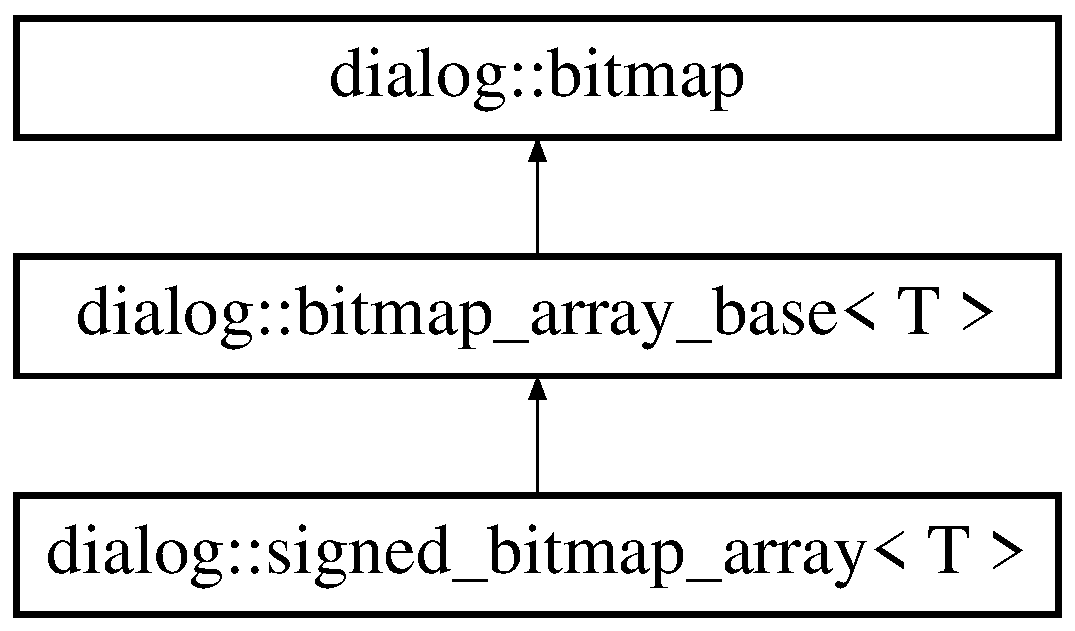
\includegraphics[height=3.000000cm]{classdialog_1_1signed__bitmap__array}
\end{center}
\end{figure}
\subsection*{Public Types}
\begin{DoxyCompactItemize}
\item 
\mbox{\Hypertarget{classdialog_1_1signed__bitmap__array_a24345e1fc4edb3caa6cf70d64b8c1270}\label{classdialog_1_1signed__bitmap__array_a24345e1fc4edb3caa6cf70d64b8c1270}} 
typedef \hyperlink{classdialog_1_1bitmap__array__base}{bitmap\+\_\+array\+\_\+base}$<$ T $>$\+::size\+\_\+type {\bfseries size\+\_\+type}
\item 
\mbox{\Hypertarget{classdialog_1_1signed__bitmap__array_a7dd28c394c7d4bc9df361821d3b8c28c}\label{classdialog_1_1signed__bitmap__array_a7dd28c394c7d4bc9df361821d3b8c28c}} 
typedef \hyperlink{classdialog_1_1bitmap__array__base}{bitmap\+\_\+array\+\_\+base}$<$ T $>$\+::width\+\_\+type {\bfseries width\+\_\+type}
\item 
\mbox{\Hypertarget{classdialog_1_1signed__bitmap__array_a1a9389659f294a8004c013729cbd8da3}\label{classdialog_1_1signed__bitmap__array_a1a9389659f294a8004c013729cbd8da3}} 
typedef \hyperlink{classdialog_1_1bitmap__array__base}{bitmap\+\_\+array\+\_\+base}$<$ T $>$\+::pos\+\_\+type {\bfseries pos\+\_\+type}
\item 
\mbox{\Hypertarget{classdialog_1_1signed__bitmap__array_aa236323ed2af148d9cfba379cdd4a4a7}\label{classdialog_1_1signed__bitmap__array_aa236323ed2af148d9cfba379cdd4a4a7}} 
typedef ptrdiff\+\_\+t {\bfseries difference\+\_\+type}
\item 
\mbox{\Hypertarget{classdialog_1_1signed__bitmap__array_aca75e58a25ad34a6d61b14df74654d78}\label{classdialog_1_1signed__bitmap__array_aca75e58a25ad34a6d61b14df74654d78}} 
typedef T {\bfseries value\+\_\+type}
\item 
\mbox{\Hypertarget{classdialog_1_1signed__bitmap__array_a49d0a2a82f2f07f9e622c3b3fdf2fb4b}\label{classdialog_1_1signed__bitmap__array_a49d0a2a82f2f07f9e622c3b3fdf2fb4b}} 
typedef T $\ast$ {\bfseries pointer}
\item 
\mbox{\Hypertarget{classdialog_1_1signed__bitmap__array_a3da9f95f558c8c94967e2101597bb434}\label{classdialog_1_1signed__bitmap__array_a3da9f95f558c8c94967e2101597bb434}} 
typedef \hyperlink{classdialog_1_1value__reference}{value\+\_\+reference}$<$ \hyperlink{classdialog_1_1signed__bitmap__array}{signed\+\_\+bitmap\+\_\+array}$<$ T $>$ $>$ {\bfseries reference}
\item 
\mbox{\Hypertarget{classdialog_1_1signed__bitmap__array_a26814c235c8b026c5ec797a0b427ee02}\label{classdialog_1_1signed__bitmap__array_a26814c235c8b026c5ec797a0b427ee02}} 
typedef \hyperlink{classdialog_1_1bitmap__array__iterator}{bitmap\+\_\+array\+\_\+iterator}$<$ \hyperlink{classdialog_1_1signed__bitmap__array}{signed\+\_\+bitmap\+\_\+array}$<$ T $>$ $>$ {\bfseries iterator}
\item 
\mbox{\Hypertarget{classdialog_1_1signed__bitmap__array_a7ef0ffd35b73a613a67d512279d29811}\label{classdialog_1_1signed__bitmap__array_a7ef0ffd35b73a613a67d512279d29811}} 
typedef \hyperlink{classdialog_1_1const__bitmap__array__iterator}{const\+\_\+bitmap\+\_\+array\+\_\+iterator}$<$ \hyperlink{classdialog_1_1signed__bitmap__array}{signed\+\_\+bitmap\+\_\+array}$<$ T $>$ $>$ {\bfseries const\+\_\+iterator}
\item 
\mbox{\Hypertarget{classdialog_1_1signed__bitmap__array_a2bc1a1dd92892e1ff97e15f88aa1c8a9}\label{classdialog_1_1signed__bitmap__array_a2bc1a1dd92892e1ff97e15f88aa1c8a9}} 
typedef std\+::random\+\_\+access\+\_\+iterator\+\_\+tag {\bfseries iterator\+\_\+category}
\end{DoxyCompactItemize}
\subsection*{Public Member Functions}
\begin{DoxyCompactItemize}
\item 
\mbox{\Hypertarget{classdialog_1_1signed__bitmap__array_af46bd6645f69d573464069004a7fdd10}\label{classdialog_1_1signed__bitmap__array_af46bd6645f69d573464069004a7fdd10}} 
{\bfseries signed\+\_\+bitmap\+\_\+array} (size\+\_\+type num\+\_\+elements, width\+\_\+type bit\+\_\+width)
\item 
\mbox{\Hypertarget{classdialog_1_1signed__bitmap__array_ab25344992051cc9af41d075d1d6c40bd}\label{classdialog_1_1signed__bitmap__array_ab25344992051cc9af41d075d1d6c40bd}} 
{\bfseries signed\+\_\+bitmap\+\_\+array} (T $\ast$elements, size\+\_\+type num\+\_\+elements, width\+\_\+type bit\+\_\+width)
\item 
\mbox{\Hypertarget{classdialog_1_1signed__bitmap__array_ad0ca1786913ee0666c1702d6f54a3118}\label{classdialog_1_1signed__bitmap__array_ad0ca1786913ee0666c1702d6f54a3118}} 
void {\bfseries set} (pos\+\_\+type i, T value)
\item 
\mbox{\Hypertarget{classdialog_1_1signed__bitmap__array_a1a2b78610fc1284e53659c81af1d51e9}\label{classdialog_1_1signed__bitmap__array_a1a2b78610fc1284e53659c81af1d51e9}} 
T {\bfseries get} (pos\+\_\+type i) const
\item 
\mbox{\Hypertarget{classdialog_1_1signed__bitmap__array_a8f2f59f09f9279f5ee7a546798badd6f}\label{classdialog_1_1signed__bitmap__array_a8f2f59f09f9279f5ee7a546798badd6f}} 
const T {\bfseries operator\mbox{[}$\,$\mbox{]}} (const pos\+\_\+type \&i) const
\item 
\mbox{\Hypertarget{classdialog_1_1signed__bitmap__array_a68bfbf4f2a21a7bdd47d870f7c2d6323}\label{classdialog_1_1signed__bitmap__array_a68bfbf4f2a21a7bdd47d870f7c2d6323}} 
\hyperlink{classdialog_1_1value__reference}{reference} {\bfseries operator\mbox{[}$\,$\mbox{]}} (const pos\+\_\+type \&i)
\item 
\mbox{\Hypertarget{classdialog_1_1signed__bitmap__array_ae7d9dd5e73774adbe1625d829ce56fcd}\label{classdialog_1_1signed__bitmap__array_ae7d9dd5e73774adbe1625d829ce56fcd}} 
\hyperlink{classdialog_1_1bitmap__array__iterator}{iterator} {\bfseries begin} ()
\item 
\mbox{\Hypertarget{classdialog_1_1signed__bitmap__array_ae5ad81b3292f6f3916e8a9409b8f75bd}\label{classdialog_1_1signed__bitmap__array_ae5ad81b3292f6f3916e8a9409b8f75bd}} 
\hyperlink{classdialog_1_1const__bitmap__array__iterator}{const\+\_\+iterator} {\bfseries begin} () const
\item 
\mbox{\Hypertarget{classdialog_1_1signed__bitmap__array_aa77ba1c6fddf982add741843b2ca25dd}\label{classdialog_1_1signed__bitmap__array_aa77ba1c6fddf982add741843b2ca25dd}} 
\hyperlink{classdialog_1_1const__bitmap__array__iterator}{const\+\_\+iterator} {\bfseries cbegin} () const
\item 
\mbox{\Hypertarget{classdialog_1_1signed__bitmap__array_a416169196b3a63b506214b5763a2ea17}\label{classdialog_1_1signed__bitmap__array_a416169196b3a63b506214b5763a2ea17}} 
\hyperlink{classdialog_1_1bitmap__array__iterator}{iterator} {\bfseries end} ()
\item 
\mbox{\Hypertarget{classdialog_1_1signed__bitmap__array_a25c24d7f1165143360edfd4dd7dec7a1}\label{classdialog_1_1signed__bitmap__array_a25c24d7f1165143360edfd4dd7dec7a1}} 
\hyperlink{classdialog_1_1const__bitmap__array__iterator}{const\+\_\+iterator} {\bfseries end} () const
\item 
\mbox{\Hypertarget{classdialog_1_1signed__bitmap__array_a34b623b88097d0b22ee83449d15871cc}\label{classdialog_1_1signed__bitmap__array_a34b623b88097d0b22ee83449d15871cc}} 
\hyperlink{classdialog_1_1const__bitmap__array__iterator}{const\+\_\+iterator} {\bfseries cend} () const
\item 
\mbox{\Hypertarget{classdialog_1_1signed__bitmap__array_a8b0d1f5fec4ec82d047d945b8edb4970}\label{classdialog_1_1signed__bitmap__array_a8b0d1f5fec4ec82d047d945b8edb4970}} 
void {\bfseries swap} (const \hyperlink{classdialog_1_1unsigned__bitmap__array}{unsigned\+\_\+bitmap\+\_\+array}$<$ T $>$ \&other)
\end{DoxyCompactItemize}
\subsection*{Additional Inherited Members}


The documentation for this class was generated from the following file\+:\begin{DoxyCompactItemize}
\item 
/\+Users/neil/\+Documents/\+Berkeley/research/dialog/libdialog/dialog/bitmap\+\_\+array.\+h\end{DoxyCompactItemize}

\hypertarget{structdialog_1_1storage_1_1storage__mode}{}\section{dialog\+:\+:storage\+:\+:storage\+\_\+mode Struct Reference}
\label{structdialog_1_1storage_1_1storage__mode}\index{dialog\+::storage\+::storage\+\_\+mode@{dialog\+::storage\+::storage\+\_\+mode}}
\subsection*{Public Attributes}
\begin{DoxyCompactItemize}
\item 
\mbox{\Hypertarget{structdialog_1_1storage_1_1storage__mode_a0c0418906c2aa3c4ce9db2050d2862bd}\label{structdialog_1_1storage_1_1storage__mode_a0c0418906c2aa3c4ce9db2050d2862bd}} 
storage\+\_\+id {\bfseries id}
\item 
\mbox{\Hypertarget{structdialog_1_1storage_1_1storage__mode_a1839c2ef8a3c0bcde495429a88ccb37f}\label{structdialog_1_1storage_1_1storage__mode_a1839c2ef8a3c0bcde495429a88ccb37f}} 
allocate\+\_\+fn {\bfseries allocate}
\item 
\mbox{\Hypertarget{structdialog_1_1storage_1_1storage__mode_a775c5b9b7cc86fe0ef1d9ac7a4d7a3e8}\label{structdialog_1_1storage_1_1storage__mode_a775c5b9b7cc86fe0ef1d9ac7a4d7a3e8}} 
free\+\_\+fn {\bfseries free}
\item 
\mbox{\Hypertarget{structdialog_1_1storage_1_1storage__mode_a38b2c5069287cb4dcfa7ddcb68def4f8}\label{structdialog_1_1storage_1_1storage__mode_a38b2c5069287cb4dcfa7ddcb68def4f8}} 
flush\+\_\+fn {\bfseries flush}
\end{DoxyCompactItemize}


The documentation for this struct was generated from the following file\+:\begin{DoxyCompactItemize}
\item 
/\+Users/neil/\+Documents/\+Berkeley/research/dialog/libdialog/dialog/storage.\+h\end{DoxyCompactItemize}

\hypertarget{structdialog_1_1string__map_1_1string__hash}{}\section{dialog\+:\+:string\+\_\+map$<$ V $>$\+:\+:string\+\_\+hash Struct Reference}
\label{structdialog_1_1string__map_1_1string__hash}\index{dialog\+::string\+\_\+map$<$ V $>$\+::string\+\_\+hash@{dialog\+::string\+\_\+map$<$ V $>$\+::string\+\_\+hash}}
\subsection*{Static Public Member Functions}
\begin{DoxyCompactItemize}
\item 
\mbox{\Hypertarget{structdialog_1_1string__map_1_1string__hash_af3d2b4b69c436b0574ea6bc61952391a}\label{structdialog_1_1string__map_1_1string__hash_af3d2b4b69c436b0574ea6bc61952391a}} 
static uint32\+\_\+t {\bfseries hash} (const std\+::string \&str)
\end{DoxyCompactItemize}


The documentation for this struct was generated from the following file\+:\begin{DoxyCompactItemize}
\item 
/\+Users/neil/\+Documents/\+Berkeley/research/dialog/libdialog/dialog/string\+\_\+map.\+h\end{DoxyCompactItemize}

\hypertarget{classdialog_1_1string__map}{}\section{dialog\+:\+:string\+\_\+map$<$ V $>$ Class Template Reference}
\label{classdialog_1_1string__map}\index{dialog\+::string\+\_\+map$<$ V $>$@{dialog\+::string\+\_\+map$<$ V $>$}}
\subsection*{Classes}
\begin{DoxyCompactItemize}
\item 
struct \hyperlink{structdialog_1_1string__map_1_1map__entry}{map\+\_\+entry}
\item 
struct \hyperlink{structdialog_1_1string__map_1_1string__hash}{string\+\_\+hash}
\end{DoxyCompactItemize}
\subsection*{Public Member Functions}
\begin{DoxyCompactItemize}
\item 
\mbox{\Hypertarget{classdialog_1_1string__map_a1cc7d8c33334155940ed24d35cb89179}\label{classdialog_1_1string__map_a1cc7d8c33334155940ed24d35cb89179}} 
int64\+\_\+t {\bfseries put} (const std\+::string \&key, const V \&value)
\item 
\mbox{\Hypertarget{classdialog_1_1string__map_a2632213e9330871062cb565bfdf13f21}\label{classdialog_1_1string__map_a2632213e9330871062cb565bfdf13f21}} 
int64\+\_\+t {\bfseries get} (const std\+::string \&key, V \&value) const
\item 
\mbox{\Hypertarget{classdialog_1_1string__map_aeba4544f65c810f4232c1a690461401a}\label{classdialog_1_1string__map_aeba4544f65c810f4232c1a690461401a}} 
int64\+\_\+t {\bfseries get} (int64\+\_\+t idx, V \&value) const
\item 
\mbox{\Hypertarget{classdialog_1_1string__map_a455e9d6004cd0dbb9a35e15f025b0893}\label{classdialog_1_1string__map_a455e9d6004cd0dbb9a35e15f025b0893}} 
int64\+\_\+t {\bfseries remove} (const std\+::string \&key, V \&value)
\end{DoxyCompactItemize}
\subsection*{Static Public Attributes}
\begin{DoxyCompactItemize}
\item 
static const uint32\+\_\+t {\bfseries M\+A\+X\+\_\+\+B\+U\+C\+K\+E\+TS}
\end{DoxyCompactItemize}


\subsection{Member Data Documentation}
\mbox{\Hypertarget{classdialog_1_1string__map_ac909ed9a75f2bba1b41649383df1290d}\label{classdialog_1_1string__map_ac909ed9a75f2bba1b41649383df1290d}} 
\index{dialog\+::string\+\_\+map@{dialog\+::string\+\_\+map}!M\+A\+X\+\_\+\+B\+U\+C\+K\+E\+TS@{M\+A\+X\+\_\+\+B\+U\+C\+K\+E\+TS}}
\index{M\+A\+X\+\_\+\+B\+U\+C\+K\+E\+TS@{M\+A\+X\+\_\+\+B\+U\+C\+K\+E\+TS}!dialog\+::string\+\_\+map@{dialog\+::string\+\_\+map}}
\subsubsection{\texorpdfstring{M\+A\+X\+\_\+\+B\+U\+C\+K\+E\+TS}{MAX\_BUCKETS}}
{\footnotesize\ttfamily template$<$typename V$>$ \\
const uint32\+\_\+t \hyperlink{classdialog_1_1string__map}{dialog\+::string\+\_\+map}$<$ V $>$\+::M\+A\+X\+\_\+\+B\+U\+C\+K\+E\+TS\hspace{0.3cm}{\ttfamily [static]}}

{\bfseries Initial value\+:}
\begin{DoxyCode}
= sysconf(\_SC\_PAGESIZE)
    / \textcolor{keyword}{sizeof}(reflog*)
\end{DoxyCode}


The documentation for this class was generated from the following file\+:\begin{DoxyCompactItemize}
\item 
/\+Users/neil/\+Documents/\+Berkeley/research/dialog/libdialog/dialog/string\+\_\+map.\+h\end{DoxyCompactItemize}

\hypertarget{classtask__pool}{}\section{task\+\_\+pool Class Reference}
\label{classtask__pool}\index{task\+\_\+pool@{task\+\_\+pool}}
\subsection*{Public Member Functions}
\begin{DoxyCompactItemize}
\item 
\mbox{\Hypertarget{classtask__pool_aa0a3c9689f5cb58670a5b4f523452a59}\label{classtask__pool_aa0a3c9689f5cb58670a5b4f523452a59}} 
{\bfseries task\+\_\+pool} (size\+\_\+t num\+\_\+workers=1)
\item 
\mbox{\Hypertarget{classtask__pool_a1278806d5bf37f76983db19ec64712b5}\label{classtask__pool_a1278806d5bf37f76983db19ec64712b5}} 
{\footnotesize template$<$class F , class ... A\+R\+GS$>$ }\\auto {\bfseries submit} (F \&\&f, A\+R\+GS \&\&... args) -\/$>$ std\+::future$<$ typename std\+::result\+\_\+of$<$ F(A\+R\+G\+S...)$>$\+::type $>$
\end{DoxyCompactItemize}


The documentation for this class was generated from the following file\+:\begin{DoxyCompactItemize}
\item 
/\+Users/neil/\+Documents/\+Berkeley/research/dialog/libdialog/dialog/task\+\_\+pool.\+h\end{DoxyCompactItemize}

\hypertarget{classtask__queue}{}\section{task\+\_\+queue Class Reference}
\label{classtask__queue}\index{task\+\_\+queue@{task\+\_\+queue}}
\subsection*{Public Types}
\begin{DoxyCompactItemize}
\item 
\mbox{\Hypertarget{classtask__queue_a54e486a36bec1abf4df464d82f8f7c69}\label{classtask__queue_a54e486a36bec1abf4df464d82f8f7c69}} 
typedef std\+::function$<$ void()$>$ {\bfseries function\+\_\+t}
\end{DoxyCompactItemize}
\subsection*{Public Member Functions}
\begin{DoxyCompactItemize}
\item 
\hyperlink{classtask__queue_ae7cb46be591296794478488fbde3799b}{task\+\_\+queue} ()
\item 
\hyperlink{classtask__queue_a01f60d69b15bc36bced03f00b9f3d443}{$\sim$task\+\_\+queue} ()
\item 
void \hyperlink{classtask__queue_a3f49e001092757da141a3067744f6af0}{invalidate} (void)
\item 
bool \hyperlink{classtask__queue_a8febb9f611ff31bc105027c7d90784a6}{dequeue} (function\+\_\+t \&out)
\item 
{\footnotesize template$<$class F , class ... A\+R\+GS$>$ }\\auto \hyperlink{classtask__queue_ac9fce851e5f4eecd014ef0130f0db4bc}{enqueue} (F \&\&f, A\+R\+GS \&\&... args) -\/$>$ std\+::future$<$ typename std\+::result\+\_\+of$<$ F(A\+R\+G\+S...)$>$\+::type $>$
\item 
bool \hyperlink{classtask__queue_a124dd18ea98e42ae705f7835fd0c69cf}{empty} () const
\item 
void \hyperlink{classtask__queue_aded81b6de1995651057c306166c8ae8b}{clear} ()
\item 
bool \hyperlink{classtask__queue_a75e723aa9cc68a264d63b40b3ef3f280}{is\+\_\+valid} () const
\end{DoxyCompactItemize}


\subsection{Constructor \& Destructor Documentation}
\mbox{\Hypertarget{classtask__queue_ae7cb46be591296794478488fbde3799b}\label{classtask__queue_ae7cb46be591296794478488fbde3799b}} 
\index{task\+\_\+queue@{task\+\_\+queue}!task\+\_\+queue@{task\+\_\+queue}}
\index{task\+\_\+queue@{task\+\_\+queue}!task\+\_\+queue@{task\+\_\+queue}}
\subsubsection{\texorpdfstring{task\+\_\+queue()}{task\_queue()}}
{\footnotesize\ttfamily task\+\_\+queue\+::task\+\_\+queue (\begin{DoxyParamCaption}{ }\end{DoxyParamCaption})\hspace{0.3cm}{\ttfamily [inline]}}

Default constructor that initializes to a valid task queue \mbox{\Hypertarget{classtask__queue_a01f60d69b15bc36bced03f00b9f3d443}\label{classtask__queue_a01f60d69b15bc36bced03f00b9f3d443}} 
\index{task\+\_\+queue@{task\+\_\+queue}!````~task\+\_\+queue@{$\sim$task\+\_\+queue}}
\index{````~task\+\_\+queue@{$\sim$task\+\_\+queue}!task\+\_\+queue@{task\+\_\+queue}}
\subsubsection{\texorpdfstring{$\sim$task\+\_\+queue()}{~task\_queue()}}
{\footnotesize\ttfamily task\+\_\+queue\+::$\sim$task\+\_\+queue (\begin{DoxyParamCaption}{ }\end{DoxyParamCaption})\hspace{0.3cm}{\ttfamily [inline]}}

Default destructor that invalidates the task queue 

\subsection{Member Function Documentation}
\mbox{\Hypertarget{classtask__queue_aded81b6de1995651057c306166c8ae8b}\label{classtask__queue_aded81b6de1995651057c306166c8ae8b}} 
\index{task\+\_\+queue@{task\+\_\+queue}!clear@{clear}}
\index{clear@{clear}!task\+\_\+queue@{task\+\_\+queue}}
\subsubsection{\texorpdfstring{clear()}{clear()}}
{\footnotesize\ttfamily void task\+\_\+queue\+::clear (\begin{DoxyParamCaption}{ }\end{DoxyParamCaption})\hspace{0.3cm}{\ttfamily [inline]}}

Clear all items from the queue. \mbox{\Hypertarget{classtask__queue_a8febb9f611ff31bc105027c7d90784a6}\label{classtask__queue_a8febb9f611ff31bc105027c7d90784a6}} 
\index{task\+\_\+queue@{task\+\_\+queue}!dequeue@{dequeue}}
\index{dequeue@{dequeue}!task\+\_\+queue@{task\+\_\+queue}}
\subsubsection{\texorpdfstring{dequeue()}{dequeue()}}
{\footnotesize\ttfamily bool task\+\_\+queue\+::dequeue (\begin{DoxyParamCaption}\item[{function\+\_\+t \&}]{out }\end{DoxyParamCaption})\hspace{0.3cm}{\ttfamily [inline]}}

Get the first value in the queue. Will block until a value is available unless clear is called or the instance is destructed. 
\begin{DoxyParams}{Parameters}
{\em out} & A void function that will be overriden with the front of the queue \\
\hline
\end{DoxyParams}
\begin{DoxyReturn}{Returns}
Returns true if a value was successfully written to the out parameter, false otherwise. 
\end{DoxyReturn}
\mbox{\Hypertarget{classtask__queue_a124dd18ea98e42ae705f7835fd0c69cf}\label{classtask__queue_a124dd18ea98e42ae705f7835fd0c69cf}} 
\index{task\+\_\+queue@{task\+\_\+queue}!empty@{empty}}
\index{empty@{empty}!task\+\_\+queue@{task\+\_\+queue}}
\subsubsection{\texorpdfstring{empty()}{empty()}}
{\footnotesize\ttfamily bool task\+\_\+queue\+::empty (\begin{DoxyParamCaption}{ }\end{DoxyParamCaption}) const\hspace{0.3cm}{\ttfamily [inline]}}

Check whether or not the queue is empty. \begin{DoxyReturn}{Returns}
True if empty false otherwise 
\end{DoxyReturn}
\mbox{\Hypertarget{classtask__queue_ac9fce851e5f4eecd014ef0130f0db4bc}\label{classtask__queue_ac9fce851e5f4eecd014ef0130f0db4bc}} 
\index{task\+\_\+queue@{task\+\_\+queue}!enqueue@{enqueue}}
\index{enqueue@{enqueue}!task\+\_\+queue@{task\+\_\+queue}}
\subsubsection{\texorpdfstring{enqueue()}{enqueue()}}
{\footnotesize\ttfamily template$<$class F , class ... A\+R\+GS$>$ \\
auto task\+\_\+queue\+::enqueue (\begin{DoxyParamCaption}\item[{F \&\&}]{f,  }\item[{A\+R\+GS \&\&...}]{args }\end{DoxyParamCaption}) -\/$>$ std\+::future$<$typename std\+::result\+\_\+of$<$F(A\+R\+G\+S...)$>$\+::type$>$ \hspace{0.3cm}{\ttfamily [inline]}}

Push a new value onto the queue. 
\begin{DoxyParams}{Parameters}
{\em f} & The future \\
\hline
{\em args} & The arguments for the queue \\
\hline
\end{DoxyParams}
\begin{DoxyReturn}{Returns}
The future value 
\end{DoxyReturn}
\mbox{\Hypertarget{classtask__queue_a3f49e001092757da141a3067744f6af0}\label{classtask__queue_a3f49e001092757da141a3067744f6af0}} 
\index{task\+\_\+queue@{task\+\_\+queue}!invalidate@{invalidate}}
\index{invalidate@{invalidate}!task\+\_\+queue@{task\+\_\+queue}}
\subsubsection{\texorpdfstring{invalidate()}{invalidate()}}
{\footnotesize\ttfamily void task\+\_\+queue\+::invalidate (\begin{DoxyParamCaption}\item[{void}]{ }\end{DoxyParamCaption})\hspace{0.3cm}{\ttfamily [inline]}}

Invalidates task queue by obtaining a lock \mbox{\Hypertarget{classtask__queue_a75e723aa9cc68a264d63b40b3ef3f280}\label{classtask__queue_a75e723aa9cc68a264d63b40b3ef3f280}} 
\index{task\+\_\+queue@{task\+\_\+queue}!is\+\_\+valid@{is\+\_\+valid}}
\index{is\+\_\+valid@{is\+\_\+valid}!task\+\_\+queue@{task\+\_\+queue}}
\subsubsection{\texorpdfstring{is\+\_\+valid()}{is\_valid()}}
{\footnotesize\ttfamily bool task\+\_\+queue\+::is\+\_\+valid (\begin{DoxyParamCaption}{ }\end{DoxyParamCaption}) const\hspace{0.3cm}{\ttfamily [inline]}}

Checks whether or not this queue is valid. \begin{DoxyReturn}{Returns}
True if valid false otherwise 
\end{DoxyReturn}


The documentation for this class was generated from the following file\+:\begin{DoxyCompactItemize}
\item 
/\+Users/neil/\+Documents/\+Berkeley/research/dialog/libdialog/dialog/task\+\_\+pool.\+h\end{DoxyCompactItemize}

\hypertarget{structtask__type}{}\section{task\+\_\+type Struct Reference}
\label{structtask__type}\index{task\+\_\+type@{task\+\_\+type}}
\subsection*{Public Member Functions}
\begin{DoxyCompactItemize}
\item 
\mbox{\Hypertarget{structtask__type_a33487635fa4dbfbf3c0fcfd6a190db6e}\label{structtask__type_a33487635fa4dbfbf3c0fcfd6a190db6e}} 
{\footnotesize template$<$class ... A\+R\+GS$>$ }\\{\bfseries task\+\_\+type} (A\+R\+GS \&\&... args)
\end{DoxyCompactItemize}
\subsection*{Public Attributes}
\begin{DoxyCompactItemize}
\item 
\mbox{\Hypertarget{structtask__type_a3469a51c6a78e7fc71803f154d79c3de}\label{structtask__type_a3469a51c6a78e7fc71803f154d79c3de}} 
std\+::function$<$ void()$>$ {\bfseries func}
\item 
\mbox{\Hypertarget{structtask__type_a09cf233855db062772a4ec60839306c5}\label{structtask__type_a09cf233855db062772a4ec60839306c5}} 
\hyperlink{structtask__type}{task\+\_\+type} $\ast$ {\bfseries next}
\end{DoxyCompactItemize}


The documentation for this struct was generated from the following file\+:\begin{DoxyCompactItemize}
\item 
/\+Users/neil/\+Documents/\+Berkeley/research/dialog/libdialog/dialog/task\+\_\+pool.\+h\end{DoxyCompactItemize}

\hypertarget{classtask__worker}{}\section{task\+\_\+worker Class Reference}
\label{classtask__worker}\index{task\+\_\+worker@{task\+\_\+worker}}
\subsection*{Public Member Functions}
\begin{DoxyCompactItemize}
\item 
\hyperlink{classtask__worker_add80ef340c383360fe6ac99f048a7212}{task\+\_\+worker} (\hyperlink{classtask__queue}{task\+\_\+queue} \&queue)
\item 
\hyperlink{classtask__worker_ade29daf48fef6c87172df511b73fb4ff}{$\sim$task\+\_\+worker} ()
\item 
void \hyperlink{classtask__worker_aa33aec83ef4e75f6a715176a31913d70}{start} ()
\item 
void \hyperlink{classtask__worker_aaa4b11b564b47d366e3acbe0e8205595}{stop} ()
\end{DoxyCompactItemize}


\subsection{Constructor \& Destructor Documentation}
\mbox{\Hypertarget{classtask__worker_add80ef340c383360fe6ac99f048a7212}\label{classtask__worker_add80ef340c383360fe6ac99f048a7212}} 
\index{task\+\_\+worker@{task\+\_\+worker}!task\+\_\+worker@{task\+\_\+worker}}
\index{task\+\_\+worker@{task\+\_\+worker}!task\+\_\+worker@{task\+\_\+worker}}
\subsubsection{\texorpdfstring{task\+\_\+worker()}{task\_worker()}}
{\footnotesize\ttfamily task\+\_\+worker\+::task\+\_\+worker (\begin{DoxyParamCaption}\item[{\hyperlink{classtask__queue}{task\+\_\+queue} \&}]{queue }\end{DoxyParamCaption})\hspace{0.3cm}{\ttfamily [inline]}}

Default constructor that initalizes work to a queue of tasks to do \mbox{\Hypertarget{classtask__worker_ade29daf48fef6c87172df511b73fb4ff}\label{classtask__worker_ade29daf48fef6c87172df511b73fb4ff}} 
\index{task\+\_\+worker@{task\+\_\+worker}!````~task\+\_\+worker@{$\sim$task\+\_\+worker}}
\index{````~task\+\_\+worker@{$\sim$task\+\_\+worker}!task\+\_\+worker@{task\+\_\+worker}}
\subsubsection{\texorpdfstring{$\sim$task\+\_\+worker()}{~task\_worker()}}
{\footnotesize\ttfamily task\+\_\+worker\+::$\sim$task\+\_\+worker (\begin{DoxyParamCaption}{ }\end{DoxyParamCaption})\hspace{0.3cm}{\ttfamily [inline]}}

Default destructor that stops all the tasks on the queue 

\subsection{Member Function Documentation}
\mbox{\Hypertarget{classtask__worker_aa33aec83ef4e75f6a715176a31913d70}\label{classtask__worker_aa33aec83ef4e75f6a715176a31913d70}} 
\index{task\+\_\+worker@{task\+\_\+worker}!start@{start}}
\index{start@{start}!task\+\_\+worker@{task\+\_\+worker}}
\subsubsection{\texorpdfstring{start()}{start()}}
{\footnotesize\ttfamily void task\+\_\+worker\+::start (\begin{DoxyParamCaption}{ }\end{DoxyParamCaption})\hspace{0.3cm}{\ttfamily [inline]}}

Starts worker on a new thread and performs each task on the queue \mbox{\Hypertarget{classtask__worker_aaa4b11b564b47d366e3acbe0e8205595}\label{classtask__worker_aaa4b11b564b47d366e3acbe0e8205595}} 
\index{task\+\_\+worker@{task\+\_\+worker}!stop@{stop}}
\index{stop@{stop}!task\+\_\+worker@{task\+\_\+worker}}
\subsubsection{\texorpdfstring{stop()}{stop()}}
{\footnotesize\ttfamily void task\+\_\+worker\+::stop (\begin{DoxyParamCaption}{ }\end{DoxyParamCaption})\hspace{0.3cm}{\ttfamily [inline]}}

Joins all of the workers and their work if possible 

The documentation for this class was generated from the following file\+:\begin{DoxyCompactItemize}
\item 
/\+Users/neil/\+Documents/\+Berkeley/research/dialog/libdialog/dialog/task\+\_\+pool.\+h\end{DoxyCompactItemize}

\hypertarget{structdialog_1_1thread__info}{}\section{dialog\+:\+:thread\+\_\+info Struct Reference}
\label{structdialog_1_1thread__info}\index{dialog\+::thread\+\_\+info@{dialog\+::thread\+\_\+info}}
\subsection*{Public Attributes}
\begin{DoxyCompactItemize}
\item 
\mbox{\Hypertarget{structdialog_1_1thread__info_ace84a765e1502b2549d1905cbc75e553}\label{structdialog_1_1thread__info_ace84a765e1502b2549d1905cbc75e553}} 
std\+::thread\+::id {\bfseries tid}
\item 
\mbox{\Hypertarget{structdialog_1_1thread__info_acd0aee6a0e151876eec6821cb934c6bd}\label{structdialog_1_1thread__info_acd0aee6a0e151876eec6821cb934c6bd}} 
atomic\+::type$<$ bool $>$ {\bfseries valid}
\end{DoxyCompactItemize}


The documentation for this struct was generated from the following file\+:\begin{DoxyCompactItemize}
\item 
/\+Users/neil/\+Documents/\+Berkeley/research/dialog/libdialog/dialog/thread\+\_\+manager.\+h\end{DoxyCompactItemize}

\hypertarget{classdialog_1_1thread__manager}{}\section{dialog\+:\+:thread\+\_\+manager Class Reference}
\label{classdialog_1_1thread__manager}\index{dialog\+::thread\+\_\+manager@{dialog\+::thread\+\_\+manager}}
\subsection*{Static Public Member Functions}
\begin{DoxyCompactItemize}
\item 
\mbox{\Hypertarget{classdialog_1_1thread__manager_a18e7d2c9ae2a24f9da7fa3332e3f38b4}\label{classdialog_1_1thread__manager_a18e7d2c9ae2a24f9da7fa3332e3f38b4}} 
static int {\bfseries register\+\_\+thread} ()
\item 
\mbox{\Hypertarget{classdialog_1_1thread__manager_a2b4200174cd631269ad163eb86cf62da}\label{classdialog_1_1thread__manager_a2b4200174cd631269ad163eb86cf62da}} 
static int {\bfseries deregister\+\_\+thread} ()
\item 
\mbox{\Hypertarget{classdialog_1_1thread__manager_a40409126eb9acc60cd0db5dcec5c3989}\label{classdialog_1_1thread__manager_a40409126eb9acc60cd0db5dcec5c3989}} 
static int {\bfseries get\+\_\+id} ()
\item 
\mbox{\Hypertarget{classdialog_1_1thread__manager_abbb25c0f4a3547b80a1a838104346eff}\label{classdialog_1_1thread__manager_abbb25c0f4a3547b80a1a838104346eff}} 
static int {\bfseries get\+\_\+max\+\_\+concurrency} ()
\item 
\mbox{\Hypertarget{classdialog_1_1thread__manager_a6ebc44ebf3c68ea11b554afb502a18cc}\label{classdialog_1_1thread__manager_a6ebc44ebf3c68ea11b554afb502a18cc}} 
static void {\bfseries set\+\_\+max\+\_\+concurrency} (int max\+\_\+concurrency)
\end{DoxyCompactItemize}


The documentation for this class was generated from the following file\+:\begin{DoxyCompactItemize}
\item 
/\+Users/neil/\+Documents/\+Berkeley/research/dialog/libdialog/dialog/thread\+\_\+manager.\+h\end{DoxyCompactItemize}

\hypertarget{classdialog_1_1index_1_1tiered__index}{}\section{dialog\+:\+:index\+:\+:tiered\+\_\+index$<$ T, K, D, stats $>$ Class Template Reference}
\label{classdialog_1_1index_1_1tiered__index}\index{dialog\+::index\+::tiered\+\_\+index$<$ T, K, D, stats $>$@{dialog\+::index\+::tiered\+\_\+index$<$ T, K, D, stats $>$}}
\subsection*{Public Types}
\begin{DoxyCompactItemize}
\item 
\mbox{\Hypertarget{classdialog_1_1index_1_1tiered__index_afb4ce4f2ba6d376549294eff5732ed52}\label{classdialog_1_1index_1_1tiered__index_afb4ce4f2ba6d376549294eff5732ed52}} 
typedef \hyperlink{classdialog_1_1index_1_1tiered__index}{tiered\+\_\+index}$<$ T, K, D -\/ 1, stats $>$ {\bfseries child\+\_\+type}
\item 
\mbox{\Hypertarget{classdialog_1_1index_1_1tiered__index_a2e1ed20ae7f61676e6b4015845a3ea5f}\label{classdialog_1_1index_1_1tiered__index_a2e1ed20ae7f61676e6b4015845a3ea5f}} 
typedef \hyperlink{classdialog_1_1index_1_1indexlet}{indexlet}$<$ \hyperlink{classdialog_1_1index_1_1tiered__index}{child\+\_\+type}, K $>$ {\bfseries idx\+\_\+type}
\end{DoxyCompactItemize}
\subsection*{Public Member Functions}
\begin{DoxyCompactItemize}
\item 
\mbox{\Hypertarget{classdialog_1_1index_1_1tiered__index_ab909933b66402ddec5491ca0f6ac28df}\label{classdialog_1_1index_1_1tiered__index_ab909933b66402ddec5491ca0f6ac28df}} 
T $\ast$ {\bfseries operator\mbox{[}$\,$\mbox{]}} (const uint64\+\_\+t key)
\item 
\mbox{\Hypertarget{classdialog_1_1index_1_1tiered__index_a6aa03fb0e9279385b591f0d7955436ac}\label{classdialog_1_1index_1_1tiered__index_a6aa03fb0e9279385b591f0d7955436ac}} 
{\footnotesize template$<$typename update , typename ... update\+\_\+args$>$ }\\T $\ast$ {\bfseries operator()} (const uint64\+\_\+t key, update \&\&u, update\+\_\+args \&\&... args)
\item 
\mbox{\Hypertarget{classdialog_1_1index_1_1tiered__index_a66697fc228452ff109c93903b9f7a6f6}\label{classdialog_1_1index_1_1tiered__index_a66697fc228452ff109c93903b9f7a6f6}} 
T $\ast$ {\bfseries at} (const uint64\+\_\+t key) const
\item 
\mbox{\Hypertarget{classdialog_1_1index_1_1tiered__index_a39be7166eb13bbaaf053ac4977f10d02}\label{classdialog_1_1index_1_1tiered__index_a39be7166eb13bbaaf053ac4977f10d02}} 
\hyperlink{classdialog_1_1index_1_1tiered__index}{child\+\_\+type} $\ast$ {\bfseries get\+\_\+or\+\_\+create\+\_\+child} (const uint64\+\_\+t k)
\item 
\mbox{\Hypertarget{classdialog_1_1index_1_1tiered__index_a8ed6927b1a06398a5af533531f460048}\label{classdialog_1_1index_1_1tiered__index_a8ed6927b1a06398a5af533531f460048}} 
\hyperlink{classdialog_1_1index_1_1tiered__index}{child\+\_\+type} $\ast$ {\bfseries get\+\_\+child} (const uint64\+\_\+t k) const
\item 
\mbox{\Hypertarget{classdialog_1_1index_1_1tiered__index_af308248d15efc5ce3edc888adfd6e389}\label{classdialog_1_1index_1_1tiered__index_af308248d15efc5ce3edc888adfd6e389}} 
stats $\ast$ {\bfseries get\+\_\+stats} (const uint64\+\_\+t key, const uint64\+\_\+t depth)
\item 
\mbox{\Hypertarget{classdialog_1_1index_1_1tiered__index_ae89ab8dc5e28975b15419d352f239cb8}\label{classdialog_1_1index_1_1tiered__index_ae89ab8dc5e28975b15419d352f239cb8}} 
stats $\ast$ {\bfseries get\+\_\+stats} ()
\item 
\mbox{\Hypertarget{classdialog_1_1index_1_1tiered__index_ae1764ad9f03dc9d5fd608e7c3d327b1a}\label{classdialog_1_1index_1_1tiered__index_ae1764ad9f03dc9d5fd608e7c3d327b1a}} 
{\footnotesize template$<$typename update , typename ... update\+\_\+args$>$ }\\void {\bfseries update\+\_\+stats} (const uint64\+\_\+t key, update \&\&u, update\+\_\+args \&\&... args)
\end{DoxyCompactItemize}
\subsection*{Static Public Attributes}
\begin{DoxyCompactItemize}
\item 
\mbox{\Hypertarget{classdialog_1_1index_1_1tiered__index_a11c55b5e24ed685f71dcdc6e5e52ed5d}\label{classdialog_1_1index_1_1tiered__index_a11c55b5e24ed685f71dcdc6e5e52ed5d}} 
static uint64\+\_\+t {\bfseries C\+H\+I\+L\+D\+\_\+\+B\+L\+O\+CK} = math\+\_\+utils\+::pow(K, D -\/ 1)
\end{DoxyCompactItemize}


The documentation for this class was generated from the following file\+:\begin{DoxyCompactItemize}
\item 
/\+Users/neil/\+Documents/\+Berkeley/research/dialog/libdialog/dialog/tiered\+\_\+index.\+h\end{DoxyCompactItemize}

\hypertarget{classdialog_1_1index_1_1tiered__index_3_01_t_00_01_k_00_011_00_01stats_01_4}{}\section{dialog\+:\+:index\+:\+:tiered\+\_\+index$<$ T, K, 1, stats $>$ Class Template Reference}
\label{classdialog_1_1index_1_1tiered__index_3_01_t_00_01_k_00_011_00_01stats_01_4}\index{dialog\+::index\+::tiered\+\_\+index$<$ T, K, 1, stats $>$@{dialog\+::index\+::tiered\+\_\+index$<$ T, K, 1, stats $>$}}
\subsection*{Public Types}
\begin{DoxyCompactItemize}
\item 
\mbox{\Hypertarget{classdialog_1_1index_1_1tiered__index_3_01_t_00_01_k_00_011_00_01stats_01_4_a7419724958204de6ddec8317cf49e814}\label{classdialog_1_1index_1_1tiered__index_3_01_t_00_01_k_00_011_00_01stats_01_4_a7419724958204de6ddec8317cf49e814}} 
typedef T {\bfseries child\+\_\+type}
\item 
\mbox{\Hypertarget{classdialog_1_1index_1_1tiered__index_3_01_t_00_01_k_00_011_00_01stats_01_4_a6646cfb695409c3bf88e783aa60ce99d}\label{classdialog_1_1index_1_1tiered__index_3_01_t_00_01_k_00_011_00_01stats_01_4_a6646cfb695409c3bf88e783aa60ce99d}} 
typedef \hyperlink{classdialog_1_1index_1_1indexlet}{indexlet}$<$ T, K $>$ {\bfseries idx\+\_\+type}
\end{DoxyCompactItemize}
\subsection*{Public Member Functions}
\begin{DoxyCompactItemize}
\item 
\mbox{\Hypertarget{classdialog_1_1index_1_1tiered__index_3_01_t_00_01_k_00_011_00_01stats_01_4_a575da4528e82b491f809ea3a63b4e472}\label{classdialog_1_1index_1_1tiered__index_3_01_t_00_01_k_00_011_00_01stats_01_4_a575da4528e82b491f809ea3a63b4e472}} 
T $\ast$ {\bfseries operator\mbox{[}$\,$\mbox{]}} (const uint64\+\_\+t key)
\item 
\mbox{\Hypertarget{classdialog_1_1index_1_1tiered__index_3_01_t_00_01_k_00_011_00_01stats_01_4_a5ff6245b3e64164336240d226c6c5b60}\label{classdialog_1_1index_1_1tiered__index_3_01_t_00_01_k_00_011_00_01stats_01_4_a5ff6245b3e64164336240d226c6c5b60}} 
{\footnotesize template$<$typename update , typename ... update\+\_\+args$>$ }\\T $\ast$ {\bfseries operator()} (const uint64\+\_\+t key, update \&\&u, update\+\_\+args \&\&... args)
\item 
\mbox{\Hypertarget{classdialog_1_1index_1_1tiered__index_3_01_t_00_01_k_00_011_00_01stats_01_4_a8ee212cbd6e2e566b1dae4ba6baf7f19}\label{classdialog_1_1index_1_1tiered__index_3_01_t_00_01_k_00_011_00_01stats_01_4_a8ee212cbd6e2e566b1dae4ba6baf7f19}} 
T $\ast$ {\bfseries at} (const uint64\+\_\+t key) const
\item 
\mbox{\Hypertarget{classdialog_1_1index_1_1tiered__index_3_01_t_00_01_k_00_011_00_01stats_01_4_a257e903a3b97376075dad8a7339c478a}\label{classdialog_1_1index_1_1tiered__index_3_01_t_00_01_k_00_011_00_01stats_01_4_a257e903a3b97376075dad8a7339c478a}} 
child\+\_\+type $\ast$ {\bfseries get\+\_\+or\+\_\+create\+\_\+child} (const uint64\+\_\+t k)
\item 
\mbox{\Hypertarget{classdialog_1_1index_1_1tiered__index_3_01_t_00_01_k_00_011_00_01stats_01_4_a4050e025ebfdab1f4fdff7d37945fd62}\label{classdialog_1_1index_1_1tiered__index_3_01_t_00_01_k_00_011_00_01stats_01_4_a4050e025ebfdab1f4fdff7d37945fd62}} 
child\+\_\+type $\ast$ {\bfseries get\+\_\+child} (const uint64\+\_\+t k) const
\item 
\mbox{\Hypertarget{classdialog_1_1index_1_1tiered__index_3_01_t_00_01_k_00_011_00_01stats_01_4_af8fcd703463423d5536121eba5125f13}\label{classdialog_1_1index_1_1tiered__index_3_01_t_00_01_k_00_011_00_01stats_01_4_af8fcd703463423d5536121eba5125f13}} 
stats $\ast$ {\bfseries get\+\_\+stats} (const uint64\+\_\+t key, const uint64\+\_\+t depth)
\item 
\mbox{\Hypertarget{classdialog_1_1index_1_1tiered__index_3_01_t_00_01_k_00_011_00_01stats_01_4_aea12d5b19bfde3e9da8f51152e014e63}\label{classdialog_1_1index_1_1tiered__index_3_01_t_00_01_k_00_011_00_01stats_01_4_aea12d5b19bfde3e9da8f51152e014e63}} 
stats $\ast$ {\bfseries get\+\_\+stats} (const uint64\+\_\+t key)
\end{DoxyCompactItemize}


The documentation for this class was generated from the following file\+:\begin{DoxyCompactItemize}
\item 
/\+Users/neil/\+Documents/\+Berkeley/research/dialog/libdialog/dialog/tiered\+\_\+index.\+h\end{DoxyCompactItemize}

\hypertarget{structdialog_1_1monitor_1_1trigger}{}\section{dialog\+:\+:monitor\+:\+:trigger Struct Reference}
\label{structdialog_1_1monitor_1_1trigger}\index{dialog\+::monitor\+::trigger@{dialog\+::monitor\+::trigger}}
\subsection*{Public Member Functions}
\begin{DoxyCompactItemize}
\item 
\mbox{\Hypertarget{structdialog_1_1monitor_1_1trigger_a47a107ae96c7562efc4dc6a6bfd8de2d}\label{structdialog_1_1monitor_1_1trigger_a47a107ae96c7562efc4dc6a6bfd8de2d}} 
{\bfseries trigger} (const std\+::string \&trigger\+\_\+name, const std\+::string \&filter\+\_\+name, const std\+::string \&trigger\+\_\+expr, aggregate\+\_\+id agg, const std\+::string \&field\+\_\+name, size\+\_\+t field\+\_\+idx, const \hyperlink{structdialog_1_1data__type}{data\+\_\+type} \&field\+\_\+type, relop\+\_\+id op, const \hyperlink{classdialog_1_1numeric}{numeric} \&threshold)
\item 
\mbox{\Hypertarget{structdialog_1_1monitor_1_1trigger_ab601fa72f197b4a443b49f1ff848d9b0}\label{structdialog_1_1monitor_1_1trigger_ab601fa72f197b4a443b49f1ff848d9b0}} 
\hyperlink{classdialog_1_1aggregate}{aggregate} {\bfseries create\+\_\+aggregate} ()
\item 
\mbox{\Hypertarget{structdialog_1_1monitor_1_1trigger_a98592f07ce3e456fb8f0cc390eaec834}\label{structdialog_1_1monitor_1_1trigger_a98592f07ce3e456fb8f0cc390eaec834}} 
std\+::string {\bfseries trigger\+\_\+name} () const
\item 
\mbox{\Hypertarget{structdialog_1_1monitor_1_1trigger_acdb506aaddd9c81cb214c61ccd26029d}\label{structdialog_1_1monitor_1_1trigger_acdb506aaddd9c81cb214c61ccd26029d}} 
std\+::string {\bfseries filter\+\_\+name} () const
\item 
\mbox{\Hypertarget{structdialog_1_1monitor_1_1trigger_afd91382a9a9819faba0b5c725f1c75e4}\label{structdialog_1_1monitor_1_1trigger_afd91382a9a9819faba0b5c725f1c75e4}} 
std\+::string {\bfseries trigger\+\_\+expr} () const
\item 
\mbox{\Hypertarget{structdialog_1_1monitor_1_1trigger_a6160169b3d1637d1b749b3691d6e305b}\label{structdialog_1_1monitor_1_1trigger_a6160169b3d1637d1b749b3691d6e305b}} 
aggregate\+\_\+id {\bfseries agg\+\_\+id} () const
\item 
\mbox{\Hypertarget{structdialog_1_1monitor_1_1trigger_a2ccad4bdc03513f13d42c8d482623413}\label{structdialog_1_1monitor_1_1trigger_a2ccad4bdc03513f13d42c8d482623413}} 
size\+\_\+t {\bfseries field\+\_\+idx} () const
\item 
\mbox{\Hypertarget{structdialog_1_1monitor_1_1trigger_ac52419ecb79710fc202f22bc42124a95}\label{structdialog_1_1monitor_1_1trigger_ac52419ecb79710fc202f22bc42124a95}} 
\hyperlink{structdialog_1_1data__type}{data\+\_\+type} {\bfseries field\+\_\+type} () const
\item 
\mbox{\Hypertarget{structdialog_1_1monitor_1_1trigger_a97a5f720df3e16c46ceff3280f51b01a}\label{structdialog_1_1monitor_1_1trigger_a97a5f720df3e16c46ceff3280f51b01a}} 
relop\+\_\+id {\bfseries op} () const
\item 
\mbox{\Hypertarget{structdialog_1_1monitor_1_1trigger_a38017ca053a1af74d51f01608c732c10}\label{structdialog_1_1monitor_1_1trigger_a38017ca053a1af74d51f01608c732c10}} 
const \hyperlink{classdialog_1_1numeric}{numeric} {\bfseries threshold} () const
\item 
\mbox{\Hypertarget{structdialog_1_1monitor_1_1trigger_a564af6d26c3978da551e16ad575e5285}\label{structdialog_1_1monitor_1_1trigger_a564af6d26c3978da551e16ad575e5285}} 
\hyperlink{classdialog_1_1numeric}{numeric} {\bfseries zero} ()
\item 
\mbox{\Hypertarget{structdialog_1_1monitor_1_1trigger_aeaae61bd2b90a7a2d6f31d7fbbda3068}\label{structdialog_1_1monitor_1_1trigger_aeaae61bd2b90a7a2d6f31d7fbbda3068}} 
\hyperlink{classdialog_1_1numeric}{numeric} {\bfseries agg} (const \hyperlink{classdialog_1_1numeric}{numeric} \&a, const \hyperlink{classdialog_1_1schema__snapshot}{schema\+\_\+snapshot} \&s, void $\ast$\hyperlink{structdialog_1_1data}{data})
\item 
\mbox{\Hypertarget{structdialog_1_1monitor_1_1trigger_a8606df378f5bf9577b37eddc123fb2c0}\label{structdialog_1_1monitor_1_1trigger_a8606df378f5bf9577b37eddc123fb2c0}} 
bool {\bfseries invalidate} ()
\item 
\mbox{\Hypertarget{structdialog_1_1monitor_1_1trigger_a31b40cce5b755efed5a0fa8d0fedfcbc}\label{structdialog_1_1monitor_1_1trigger_a31b40cce5b755efed5a0fa8d0fedfcbc}} 
bool {\bfseries is\+\_\+valid} () const
\item 
\mbox{\Hypertarget{structdialog_1_1monitor_1_1trigger_a632d24dac88cb3885bb5f5972db29c42}\label{structdialog_1_1monitor_1_1trigger_a632d24dac88cb3885bb5f5972db29c42}} 
std\+::string {\bfseries to\+\_\+string} () const
\end{DoxyCompactItemize}


The documentation for this struct was generated from the following file\+:\begin{DoxyCompactItemize}
\item 
/\+Users/neil/\+Documents/\+Berkeley/research/dialog/libdialog/dialog/trigger.\+h\end{DoxyCompactItemize}

\hypertarget{structdialog_1_1trigger__info}{}\section{dialog\+:\+:trigger\+\_\+info Struct Reference}
\label{structdialog_1_1trigger__info}\index{dialog\+::trigger\+\_\+info@{dialog\+::trigger\+\_\+info}}
\subsection*{Public Member Functions}
\begin{DoxyCompactItemize}
\item 
\mbox{\Hypertarget{structdialog_1_1trigger__info_acd6fb53454c63a2203b558be1c7bd4fa}\label{structdialog_1_1trigger__info_acd6fb53454c63a2203b558be1c7bd4fa}} 
{\bfseries trigger\+\_\+info} (const std\+::string \&trigger\+\_\+name, const std\+::string \&filter\+\_\+name, aggregate\+\_\+id agg\+\_\+id, const std\+::string \&field\+\_\+name, relop\+\_\+id op, const \hyperlink{classdialog_1_1numeric}{numeric} \&threshold)
\item 
\mbox{\Hypertarget{structdialog_1_1trigger__info_a3ac73c8c9986a395a1c4a247b5bc8af4}\label{structdialog_1_1trigger__info_a3ac73c8c9986a395a1c4a247b5bc8af4}} 
const std\+::string \& {\bfseries trigger\+\_\+name} () const
\item 
\mbox{\Hypertarget{structdialog_1_1trigger__info_a6b66660e86e8217ad842cd719ab1391f}\label{structdialog_1_1trigger__info_a6b66660e86e8217ad842cd719ab1391f}} 
const std\+::string \& {\bfseries filter\+\_\+name} () const
\item 
\mbox{\Hypertarget{structdialog_1_1trigger__info_a3b44b2fcd5484841ca1d902810b39342}\label{structdialog_1_1trigger__info_a3b44b2fcd5484841ca1d902810b39342}} 
aggregate\+\_\+id {\bfseries agg\+\_\+id} () const
\item 
\mbox{\Hypertarget{structdialog_1_1trigger__info_add236537768fe1cce28bf8a7204592f6}\label{structdialog_1_1trigger__info_add236537768fe1cce28bf8a7204592f6}} 
relop\+\_\+id {\bfseries op} () const
\item 
\mbox{\Hypertarget{structdialog_1_1trigger__info_a3c414f4881add3e4da377028c212ef47}\label{structdialog_1_1trigger__info_a3c414f4881add3e4da377028c212ef47}} 
const std\+::string \& {\bfseries field\+\_\+name} () const
\item 
\mbox{\Hypertarget{structdialog_1_1trigger__info_a79d7e14277aee7105aa8faf983e0a601}\label{structdialog_1_1trigger__info_a79d7e14277aee7105aa8faf983e0a601}} 
const \hyperlink{classdialog_1_1numeric}{numeric} \& {\bfseries threshold} () const
\end{DoxyCompactItemize}


The documentation for this struct was generated from the following file\+:\begin{DoxyCompactItemize}
\item 
/\+Users/neil/\+Documents/\+Berkeley/research/dialog/libdialog/dialog/table\+\_\+metadata.\+h\end{DoxyCompactItemize}

\hypertarget{structdialog_1_1trigger__lex__token}{}\section{dialog\+:\+:trigger\+\_\+lex\+\_\+token Struct Reference}
\label{structdialog_1_1trigger__lex__token}\index{dialog\+::trigger\+\_\+lex\+\_\+token@{dialog\+::trigger\+\_\+lex\+\_\+token}}
\subsection*{Public Member Functions}
\begin{DoxyCompactItemize}
\item 
\mbox{\Hypertarget{structdialog_1_1trigger__lex__token_a8c94fc6b0ca2e714fc6801152f3f9e73}\label{structdialog_1_1trigger__lex__token_a8c94fc6b0ca2e714fc6801152f3f9e73}} 
{\bfseries trigger\+\_\+lex\+\_\+token} (int i, const std\+::string \&val)
\end{DoxyCompactItemize}
\subsection*{Public Attributes}
\begin{DoxyCompactItemize}
\item 
\mbox{\Hypertarget{structdialog_1_1trigger__lex__token_a406d80ed3ab6c06f080936865223a1ae}\label{structdialog_1_1trigger__lex__token_a406d80ed3ab6c06f080936865223a1ae}} 
int {\bfseries id}
\item 
\mbox{\Hypertarget{structdialog_1_1trigger__lex__token_a3802f48f7934dcbcd483bbb5c21b170d}\label{structdialog_1_1trigger__lex__token_a3802f48f7934dcbcd483bbb5c21b170d}} 
std\+::string {\bfseries value}
\end{DoxyCompactItemize}


The documentation for this struct was generated from the following file\+:\begin{DoxyCompactItemize}
\item 
/\+Users/neil/\+Documents/\+Berkeley/research/dialog/libdialog/dialog/trigger\+\_\+parser.\+h\end{DoxyCompactItemize}

\hypertarget{classdialog_1_1trigger__lexer}{}\section{dialog\+:\+:trigger\+\_\+lexer Class Reference}
\label{classdialog_1_1trigger__lexer}\index{dialog\+::trigger\+\_\+lexer@{dialog\+::trigger\+\_\+lexer}}
\subsection*{Public Member Functions}
\begin{DoxyCompactItemize}
\item 
\mbox{\Hypertarget{classdialog_1_1trigger__lexer_a0a7a49b605d1e400e9b9413539bfb91b}\label{classdialog_1_1trigger__lexer_a0a7a49b605d1e400e9b9413539bfb91b}} 
{\bfseries trigger\+\_\+lexer} (const std\+::string \&exp)
\item 
\mbox{\Hypertarget{classdialog_1_1trigger__lexer_ab0220d33b6e19dd7f2c6be53938faabf}\label{classdialog_1_1trigger__lexer_ab0220d33b6e19dd7f2c6be53938faabf}} 
void {\bfseries str} (const std\+::string \&exp)
\item 
\mbox{\Hypertarget{classdialog_1_1trigger__lexer_a2b11ed854a1e3e6c51c82928c9aac9e9}\label{classdialog_1_1trigger__lexer_a2b11ed854a1e3e6c51c82928c9aac9e9}} 
size\+\_\+t {\bfseries pos} ()
\item 
\mbox{\Hypertarget{classdialog_1_1trigger__lexer_aeaaa5db0c6cd2b92aafca26c392d7048}\label{classdialog_1_1trigger__lexer_aeaaa5db0c6cd2b92aafca26c392d7048}} 
std\+::string {\bfseries str} ()
\item 
\mbox{\Hypertarget{classdialog_1_1trigger__lexer_a233e41048c686663994494bacdf26881}\label{classdialog_1_1trigger__lexer_a233e41048c686663994494bacdf26881}} 
const \hyperlink{structdialog_1_1trigger__lex__token}{trigger\+\_\+lex\+\_\+token} {\bfseries next\+\_\+token} ()
\end{DoxyCompactItemize}
\subsection*{Static Public Attributes}
\begin{DoxyCompactItemize}
\item 
\mbox{\Hypertarget{classdialog_1_1trigger__lexer_adf06ecddf6fef7b28af0aa32fbcb541f}\label{classdialog_1_1trigger__lexer_adf06ecddf6fef7b28af0aa32fbcb541f}} 
static const int {\bfseries I\+N\+V\+A\+L\+ID} = -\/2
\item 
\mbox{\Hypertarget{classdialog_1_1trigger__lexer_af5911c5c3ace43057522ceba49590fcb}\label{classdialog_1_1trigger__lexer_af5911c5c3ace43057522ceba49590fcb}} 
static const int {\bfseries E\+ND} = -\/1
\item 
\mbox{\Hypertarget{classdialog_1_1trigger__lexer_aa5e047f50c2134563f363fcfcf118068}\label{classdialog_1_1trigger__lexer_aa5e047f50c2134563f363fcfcf118068}} 
static const int {\bfseries L\+E\+FT} = 1
\item 
\mbox{\Hypertarget{classdialog_1_1trigger__lexer_ac85684104fecfda94ce67f18800fbe84}\label{classdialog_1_1trigger__lexer_ac85684104fecfda94ce67f18800fbe84}} 
static const int {\bfseries R\+I\+G\+HT} = 2
\item 
\mbox{\Hypertarget{classdialog_1_1trigger__lexer_a93512c86a07ca4f4db552b3caf4a18d0}\label{classdialog_1_1trigger__lexer_a93512c86a07ca4f4db552b3caf4a18d0}} 
static const int {\bfseries O\+P\+E\+R\+A\+T\+OR} = 3
\item 
\mbox{\Hypertarget{classdialog_1_1trigger__lexer_a2f1c98e898271eb595ab23d9f2ccb143}\label{classdialog_1_1trigger__lexer_a2f1c98e898271eb595ab23d9f2ccb143}} 
static const int {\bfseries O\+P\+E\+R\+A\+ND} = 4
\end{DoxyCompactItemize}


The documentation for this class was generated from the following file\+:\begin{DoxyCompactItemize}
\item 
/\+Users/neil/\+Documents/\+Berkeley/research/dialog/libdialog/dialog/trigger\+\_\+parser.\+h\end{DoxyCompactItemize}

\hypertarget{classdialog_1_1trigger__parser}{}\section{dialog\+:\+:trigger\+\_\+parser Class Reference}
\label{classdialog_1_1trigger__parser}\index{dialog\+::trigger\+\_\+parser@{dialog\+::trigger\+\_\+parser}}
\subsection*{Public Member Functions}
\begin{DoxyCompactItemize}
\item 
\mbox{\Hypertarget{classdialog_1_1trigger__parser_a1ca144dc8f1524b100518ca0bce70e94}\label{classdialog_1_1trigger__parser_a1ca144dc8f1524b100518ca0bce70e94}} 
{\bfseries trigger\+\_\+parser} (const std\+::string \&exp, const \hyperlink{classdialog_1_1schema__t}{schema\+\_\+t} \&schema)
\item 
\mbox{\Hypertarget{classdialog_1_1trigger__parser_a685addc92c994e5627740933301a39fe}\label{classdialog_1_1trigger__parser_a685addc92c994e5627740933301a39fe}} 
\hyperlink{structdialog_1_1parsed__trigger}{parsed\+\_\+trigger} {\bfseries parse} ()
\end{DoxyCompactItemize}


The documentation for this class was generated from the following file\+:\begin{DoxyCompactItemize}
\item 
/\+Users/neil/\+Documents/\+Berkeley/research/dialog/libdialog/dialog/trigger\+\_\+parser.\+h\end{DoxyCompactItemize}

\hypertarget{classdialog_1_1union__record__stream}{}\section{dialog\+:\+:union\+\_\+record\+\_\+stream$<$ rstream\+\_\+t $>$ Class Template Reference}
\label{classdialog_1_1union__record__stream}\index{dialog\+::union\+\_\+record\+\_\+stream$<$ rstream\+\_\+t $>$@{dialog\+::union\+\_\+record\+\_\+stream$<$ rstream\+\_\+t $>$}}
\subsection*{Public Types}
\begin{DoxyCompactItemize}
\item 
\mbox{\Hypertarget{classdialog_1_1union__record__stream_adc2268e097c6a87401608880db6683ad}\label{classdialog_1_1union__record__stream_adc2268e097c6a87401608880db6683ad}} 
typedef std\+::vector$<$ rstream\+\_\+t $>$ {\bfseries stream\+\_\+vector\+\_\+t}
\end{DoxyCompactItemize}
\subsection*{Public Member Functions}
\begin{DoxyCompactItemize}
\item 
\mbox{\Hypertarget{classdialog_1_1union__record__stream_a87adf97ded0c364328a8d4d6c05c67e8}\label{classdialog_1_1union__record__stream_a87adf97ded0c364328a8d4d6c05c67e8}} 
{\bfseries union\+\_\+record\+\_\+stream} (const stream\+\_\+vector\+\_\+t \&rstreams)
\item 
\mbox{\Hypertarget{classdialog_1_1union__record__stream_a5c778787a04599d1632567d875adb78f}\label{classdialog_1_1union__record__stream_a5c778787a04599d1632567d875adb78f}} 
\hyperlink{structdialog_1_1record__t}{record\+\_\+t} {\bfseries get} () const
\item 
\mbox{\Hypertarget{classdialog_1_1union__record__stream_a861d76a525e5301099a752cee7a12c39}\label{classdialog_1_1union__record__stream_a861d76a525e5301099a752cee7a12c39}} 
\hyperlink{classdialog_1_1union__record__stream}{union\+\_\+record\+\_\+stream} \& {\bfseries operator++} ()
\item 
\mbox{\Hypertarget{classdialog_1_1union__record__stream_a1dd62584b7ac4093214531ba214c21dd}\label{classdialog_1_1union__record__stream_a1dd62584b7ac4093214531ba214c21dd}} 
\hyperlink{classdialog_1_1union__record__stream}{union\+\_\+record\+\_\+stream} \& {\bfseries operator++} (int)
\item 
\mbox{\Hypertarget{classdialog_1_1union__record__stream_adfff04e32d3390cc8ca38a4e356e8d31}\label{classdialog_1_1union__record__stream_adfff04e32d3390cc8ca38a4e356e8d31}} 
bool {\bfseries has\+\_\+more} () const
\end{DoxyCompactItemize}


The documentation for this class was generated from the following file\+:\begin{DoxyCompactItemize}
\item 
/\+Users/neil/\+Documents/\+Berkeley/research/dialog/libdialog/dialog/record\+\_\+stream.\+h\end{DoxyCompactItemize}

\hypertarget{classdialog_1_1unsigned__bitmap__array}{}\section{dialog\+:\+:unsigned\+\_\+bitmap\+\_\+array$<$ T $>$ Class Template Reference}
\label{classdialog_1_1unsigned__bitmap__array}\index{dialog\+::unsigned\+\_\+bitmap\+\_\+array$<$ T $>$@{dialog\+::unsigned\+\_\+bitmap\+\_\+array$<$ T $>$}}
Inheritance diagram for dialog\+:\+:unsigned\+\_\+bitmap\+\_\+array$<$ T $>$\+:\begin{figure}[H]
\begin{center}
\leavevmode
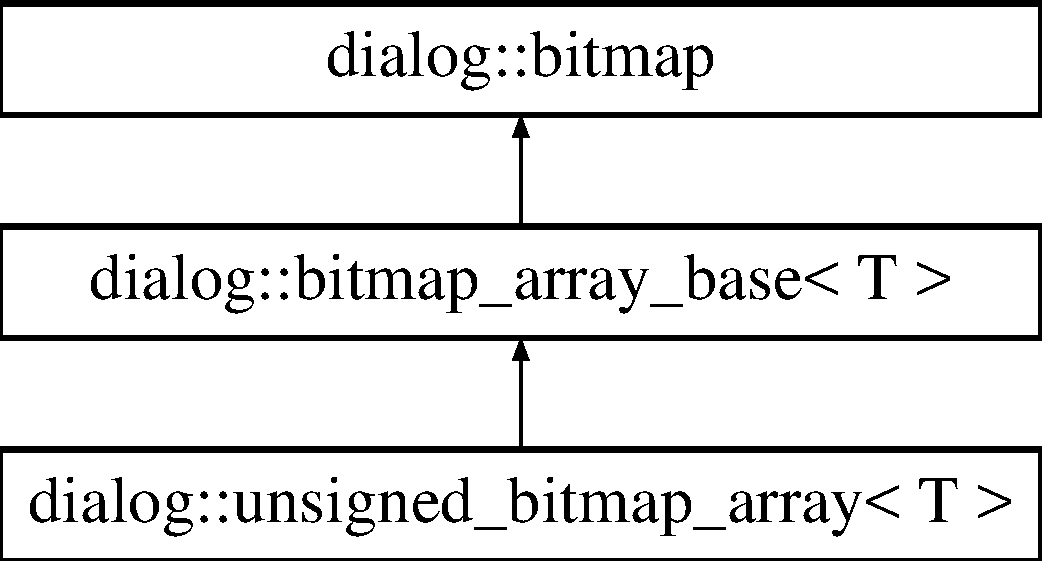
\includegraphics[height=3.000000cm]{classdialog_1_1unsigned__bitmap__array}
\end{center}
\end{figure}
\subsection*{Public Types}
\begin{DoxyCompactItemize}
\item 
\mbox{\Hypertarget{classdialog_1_1unsigned__bitmap__array_a4310b8ce4e699979c8de82dd6ec68b6c}\label{classdialog_1_1unsigned__bitmap__array_a4310b8ce4e699979c8de82dd6ec68b6c}} 
typedef \hyperlink{classdialog_1_1bitmap__array__base}{bitmap\+\_\+array\+\_\+base}$<$ T $>$\+::size\+\_\+type {\bfseries size\+\_\+type}
\item 
\mbox{\Hypertarget{classdialog_1_1unsigned__bitmap__array_a5c11af0fe1193e79f8b3b47db67a5bac}\label{classdialog_1_1unsigned__bitmap__array_a5c11af0fe1193e79f8b3b47db67a5bac}} 
typedef \hyperlink{classdialog_1_1bitmap__array__base}{bitmap\+\_\+array\+\_\+base}$<$ T $>$\+::width\+\_\+type {\bfseries width\+\_\+type}
\item 
\mbox{\Hypertarget{classdialog_1_1unsigned__bitmap__array_a9f098b2a9fb1226c3b704cd5ce427f72}\label{classdialog_1_1unsigned__bitmap__array_a9f098b2a9fb1226c3b704cd5ce427f72}} 
typedef \hyperlink{classdialog_1_1bitmap__array__base}{bitmap\+\_\+array\+\_\+base}$<$ T $>$\+::pos\+\_\+type {\bfseries pos\+\_\+type}
\item 
\mbox{\Hypertarget{classdialog_1_1unsigned__bitmap__array_a860b7fca544641f35ac7581077f41a67}\label{classdialog_1_1unsigned__bitmap__array_a860b7fca544641f35ac7581077f41a67}} 
typedef ptrdiff\+\_\+t {\bfseries difference\+\_\+type}
\item 
\mbox{\Hypertarget{classdialog_1_1unsigned__bitmap__array_a2c404d9ac20eeff687759a0b2c3a33d4}\label{classdialog_1_1unsigned__bitmap__array_a2c404d9ac20eeff687759a0b2c3a33d4}} 
typedef T {\bfseries value\+\_\+type}
\item 
\mbox{\Hypertarget{classdialog_1_1unsigned__bitmap__array_a4f1798c22124d6d6a16b36ed075ffb05}\label{classdialog_1_1unsigned__bitmap__array_a4f1798c22124d6d6a16b36ed075ffb05}} 
typedef T $\ast$ {\bfseries pointer}
\item 
\mbox{\Hypertarget{classdialog_1_1unsigned__bitmap__array_a3a8d29bcd0353f355f8687cb5fb97423}\label{classdialog_1_1unsigned__bitmap__array_a3a8d29bcd0353f355f8687cb5fb97423}} 
typedef \hyperlink{classdialog_1_1value__reference}{value\+\_\+reference}$<$ \hyperlink{classdialog_1_1unsigned__bitmap__array}{unsigned\+\_\+bitmap\+\_\+array}$<$ T $>$ $>$ {\bfseries reference}
\item 
\mbox{\Hypertarget{classdialog_1_1unsigned__bitmap__array_a8d54fc9d097c1af9503cd3949c242a3f}\label{classdialog_1_1unsigned__bitmap__array_a8d54fc9d097c1af9503cd3949c242a3f}} 
typedef \hyperlink{classdialog_1_1bitmap__array__iterator}{bitmap\+\_\+array\+\_\+iterator}$<$ \hyperlink{classdialog_1_1unsigned__bitmap__array}{unsigned\+\_\+bitmap\+\_\+array}$<$ T $>$ $>$ {\bfseries iterator}
\item 
\mbox{\Hypertarget{classdialog_1_1unsigned__bitmap__array_a92ee64730c694bde54130c1b3cad8b1e}\label{classdialog_1_1unsigned__bitmap__array_a92ee64730c694bde54130c1b3cad8b1e}} 
typedef \hyperlink{classdialog_1_1const__bitmap__array__iterator}{const\+\_\+bitmap\+\_\+array\+\_\+iterator}$<$ \hyperlink{classdialog_1_1unsigned__bitmap__array}{unsigned\+\_\+bitmap\+\_\+array}$<$ T $>$ $>$ {\bfseries const\+\_\+iterator}
\item 
\mbox{\Hypertarget{classdialog_1_1unsigned__bitmap__array_a1c3d2c473aee2a4738912d2bcf1a13fd}\label{classdialog_1_1unsigned__bitmap__array_a1c3d2c473aee2a4738912d2bcf1a13fd}} 
typedef std\+::random\+\_\+access\+\_\+iterator\+\_\+tag {\bfseries iterator\+\_\+category}
\end{DoxyCompactItemize}
\subsection*{Public Member Functions}
\begin{DoxyCompactItemize}
\item 
\mbox{\Hypertarget{classdialog_1_1unsigned__bitmap__array_a4d694950b177597db7699e77267350f1}\label{classdialog_1_1unsigned__bitmap__array_a4d694950b177597db7699e77267350f1}} 
{\bfseries unsigned\+\_\+bitmap\+\_\+array} (size\+\_\+type num\+\_\+elements, width\+\_\+type bit\+\_\+width)
\item 
\mbox{\Hypertarget{classdialog_1_1unsigned__bitmap__array_ab02205927de3ee2a17539fc74f59b998}\label{classdialog_1_1unsigned__bitmap__array_ab02205927de3ee2a17539fc74f59b998}} 
{\bfseries unsigned\+\_\+bitmap\+\_\+array} (T $\ast$elements, size\+\_\+type num\+\_\+elements, width\+\_\+type bit\+\_\+width)
\item 
\mbox{\Hypertarget{classdialog_1_1unsigned__bitmap__array_aa4419794d3574e0e09df023d0777ff96}\label{classdialog_1_1unsigned__bitmap__array_aa4419794d3574e0e09df023d0777ff96}} 
void {\bfseries set} (pos\+\_\+type i, T value)
\item 
\mbox{\Hypertarget{classdialog_1_1unsigned__bitmap__array_a690643f7045025e155b96d310f8ed8f8}\label{classdialog_1_1unsigned__bitmap__array_a690643f7045025e155b96d310f8ed8f8}} 
T {\bfseries get} (pos\+\_\+type i) const
\item 
\mbox{\Hypertarget{classdialog_1_1unsigned__bitmap__array_afdb24dce8a98cfbbf40eac935067b37c}\label{classdialog_1_1unsigned__bitmap__array_afdb24dce8a98cfbbf40eac935067b37c}} 
const T {\bfseries operator\mbox{[}$\,$\mbox{]}} (const pos\+\_\+type \&i) const
\item 
\mbox{\Hypertarget{classdialog_1_1unsigned__bitmap__array_ab56f8c0ec937a8b2e5eeef98bcfca23d}\label{classdialog_1_1unsigned__bitmap__array_ab56f8c0ec937a8b2e5eeef98bcfca23d}} 
\hyperlink{classdialog_1_1value__reference}{reference} {\bfseries operator\mbox{[}$\,$\mbox{]}} (const pos\+\_\+type \&i)
\item 
\mbox{\Hypertarget{classdialog_1_1unsigned__bitmap__array_a2caef77ec8403ea76166de6cdc3690e2}\label{classdialog_1_1unsigned__bitmap__array_a2caef77ec8403ea76166de6cdc3690e2}} 
\hyperlink{classdialog_1_1bitmap__array__iterator}{iterator} {\bfseries begin} ()
\item 
\mbox{\Hypertarget{classdialog_1_1unsigned__bitmap__array_a738b81321c87e8d190ea401787f986d7}\label{classdialog_1_1unsigned__bitmap__array_a738b81321c87e8d190ea401787f986d7}} 
\hyperlink{classdialog_1_1const__bitmap__array__iterator}{const\+\_\+iterator} {\bfseries begin} () const
\item 
\mbox{\Hypertarget{classdialog_1_1unsigned__bitmap__array_a3164e4fd90ceca7e70b00f5e33693d12}\label{classdialog_1_1unsigned__bitmap__array_a3164e4fd90ceca7e70b00f5e33693d12}} 
\hyperlink{classdialog_1_1const__bitmap__array__iterator}{const\+\_\+iterator} {\bfseries cbegin} () const
\item 
\mbox{\Hypertarget{classdialog_1_1unsigned__bitmap__array_a49aaa3970f574a68d4e30e901599c9c7}\label{classdialog_1_1unsigned__bitmap__array_a49aaa3970f574a68d4e30e901599c9c7}} 
\hyperlink{classdialog_1_1bitmap__array__iterator}{iterator} {\bfseries end} ()
\item 
\mbox{\Hypertarget{classdialog_1_1unsigned__bitmap__array_af25e47ec6f32be461558349229d84cef}\label{classdialog_1_1unsigned__bitmap__array_af25e47ec6f32be461558349229d84cef}} 
\hyperlink{classdialog_1_1const__bitmap__array__iterator}{const\+\_\+iterator} {\bfseries end} () const
\item 
\mbox{\Hypertarget{classdialog_1_1unsigned__bitmap__array_a88da7a686ed3f8b5d8f0b81fd6602a4b}\label{classdialog_1_1unsigned__bitmap__array_a88da7a686ed3f8b5d8f0b81fd6602a4b}} 
\hyperlink{classdialog_1_1const__bitmap__array__iterator}{const\+\_\+iterator} {\bfseries cend} () const
\item 
\mbox{\Hypertarget{classdialog_1_1unsigned__bitmap__array_a3f699e7874ada6827762558eaa542a76}\label{classdialog_1_1unsigned__bitmap__array_a3f699e7874ada6827762558eaa542a76}} 
void {\bfseries swap} (const \hyperlink{classdialog_1_1unsigned__bitmap__array}{unsigned\+\_\+bitmap\+\_\+array}$<$ T $>$ \&other)
\end{DoxyCompactItemize}
\subsection*{Additional Inherited Members}


The documentation for this class was generated from the following file\+:\begin{DoxyCompactItemize}
\item 
/\+Users/neil/\+Documents/\+Berkeley/research/dialog/libdialog/dialog/bitmap\+\_\+array.\+h\end{DoxyCompactItemize}

\hypertarget{classdialog_1_1unsized__bitmap__array}{}\section{dialog\+:\+:unsized\+\_\+bitmap\+\_\+array$<$ T $>$ Class Template Reference}
\label{classdialog_1_1unsized__bitmap__array}\index{dialog\+::unsized\+\_\+bitmap\+\_\+array$<$ T $>$@{dialog\+::unsized\+\_\+bitmap\+\_\+array$<$ T $>$}}
Inheritance diagram for dialog\+:\+:unsized\+\_\+bitmap\+\_\+array$<$ T $>$\+:\begin{figure}[H]
\begin{center}
\leavevmode
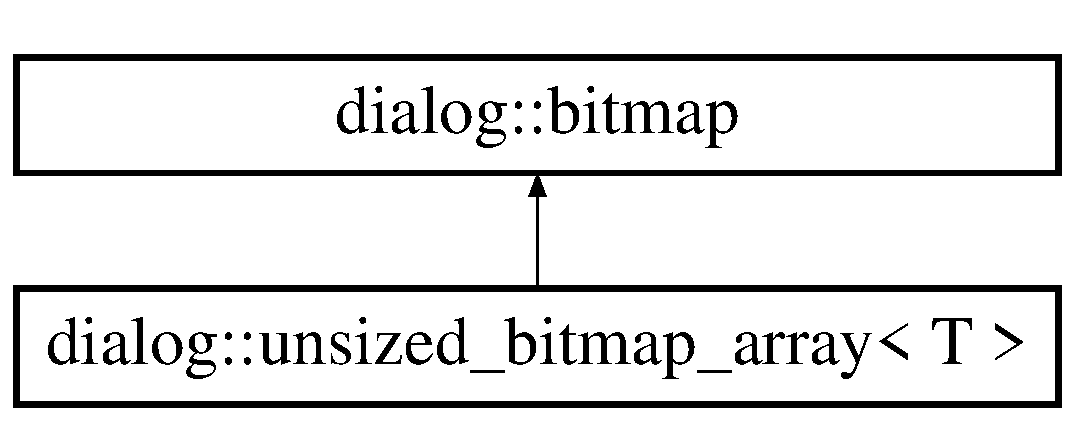
\includegraphics[height=2.000000cm]{classdialog_1_1unsized__bitmap__array}
\end{center}
\end{figure}
\subsection*{Public Types}
\begin{DoxyCompactItemize}
\item 
\mbox{\Hypertarget{classdialog_1_1unsized__bitmap__array_a4fe55f99c731168e7f95545f0a0fcd2a}\label{classdialog_1_1unsized__bitmap__array_a4fe55f99c731168e7f95545f0a0fcd2a}} 
typedef \hyperlink{classdialog_1_1bitmap__array__base}{bitmap\+\_\+array\+\_\+base}$<$ T $>$\+::size\+\_\+type {\bfseries size\+\_\+type}
\item 
\mbox{\Hypertarget{classdialog_1_1unsized__bitmap__array_ad2a52dd64f8be340d5eb8fd7f631c0e3}\label{classdialog_1_1unsized__bitmap__array_ad2a52dd64f8be340d5eb8fd7f631c0e3}} 
typedef \hyperlink{classdialog_1_1bitmap__array__base}{bitmap\+\_\+array\+\_\+base}$<$ T $>$\+::width\+\_\+type {\bfseries width\+\_\+type}
\item 
\mbox{\Hypertarget{classdialog_1_1unsized__bitmap__array_ac7ad7cccd26c107aae84ac5323fb2ce5}\label{classdialog_1_1unsized__bitmap__array_ac7ad7cccd26c107aae84ac5323fb2ce5}} 
typedef \hyperlink{classdialog_1_1bitmap__array__base}{bitmap\+\_\+array\+\_\+base}$<$ T $>$\+::pos\+\_\+type {\bfseries pos\+\_\+type}
\item 
\mbox{\Hypertarget{classdialog_1_1unsized__bitmap__array_a334227ffb88f529ae1e2d6700ad99041}\label{classdialog_1_1unsized__bitmap__array_a334227ffb88f529ae1e2d6700ad99041}} 
typedef \hyperlink{classdialog_1_1value__reference}{value\+\_\+reference}$<$ \hyperlink{classdialog_1_1unsized__bitmap__array}{unsized\+\_\+bitmap\+\_\+array}$<$ T $>$ $>$ {\bfseries reference}
\item 
\mbox{\Hypertarget{classdialog_1_1unsized__bitmap__array_a93a78d41d8baa7829e551a09236ce1ff}\label{classdialog_1_1unsized__bitmap__array_a93a78d41d8baa7829e551a09236ce1ff}} 
typedef T {\bfseries value\+\_\+type}
\end{DoxyCompactItemize}
\subsection*{Public Member Functions}
\begin{DoxyCompactItemize}
\item 
\mbox{\Hypertarget{classdialog_1_1unsized__bitmap__array_a940998b89b7e061c39ea8720aa7b3b61}\label{classdialog_1_1unsized__bitmap__array_a940998b89b7e061c39ea8720aa7b3b61}} 
{\bfseries unsized\+\_\+bitmap\+\_\+array} (const \hyperlink{classdialog_1_1unsized__bitmap__array}{unsized\+\_\+bitmap\+\_\+array} \&array)
\item 
\mbox{\Hypertarget{classdialog_1_1unsized__bitmap__array_a849b479fd6e8c67ed680695d04f4cac0}\label{classdialog_1_1unsized__bitmap__array_a849b479fd6e8c67ed680695d04f4cac0}} 
{\bfseries unsized\+\_\+bitmap\+\_\+array} (size\+\_\+type num\+\_\+elements, width\+\_\+type bit\+\_\+width)
\item 
\mbox{\Hypertarget{classdialog_1_1unsized__bitmap__array_a2c7c8fa9c04b92259ce3fa1630fdd4f2}\label{classdialog_1_1unsized__bitmap__array_a2c7c8fa9c04b92259ce3fa1630fdd4f2}} 
{\bfseries unsized\+\_\+bitmap\+\_\+array} (T $\ast$elements, size\+\_\+type num\+\_\+elements, width\+\_\+type bit\+\_\+width)
\item 
\mbox{\Hypertarget{classdialog_1_1unsized__bitmap__array_aad12c309b1d637d8c0a25546098cf717}\label{classdialog_1_1unsized__bitmap__array_aad12c309b1d637d8c0a25546098cf717}} 
void {\bfseries set} (pos\+\_\+type i, T value)
\item 
\mbox{\Hypertarget{classdialog_1_1unsized__bitmap__array_ac9dfbc9c10483e0f4d4943a0516a5f08}\label{classdialog_1_1unsized__bitmap__array_ac9dfbc9c10483e0f4d4943a0516a5f08}} 
T {\bfseries get} (pos\+\_\+type i) const
\item 
\mbox{\Hypertarget{classdialog_1_1unsized__bitmap__array_a783d5378e0f0aa1e10c10f0108feefd0}\label{classdialog_1_1unsized__bitmap__array_a783d5378e0f0aa1e10c10f0108feefd0}} 
const T {\bfseries operator\mbox{[}$\,$\mbox{]}} (const pos\+\_\+type \&i) const
\item 
\mbox{\Hypertarget{classdialog_1_1unsized__bitmap__array_ac3a92dbcf24be1eab76efcb3a5dd8d3a}\label{classdialog_1_1unsized__bitmap__array_ac3a92dbcf24be1eab76efcb3a5dd8d3a}} 
\hyperlink{classdialog_1_1value__reference}{reference} {\bfseries operator\mbox{[}$\,$\mbox{]}} (const pos\+\_\+type \&i)
\item 
virtual size\+\_\+type \hyperlink{classdialog_1_1unsized__bitmap__array_a3c6dfec187c0ecad49d562c2b081ec6a}{serialize} (std\+::ostream \&out) override
\item 
virtual size\+\_\+type \hyperlink{classdialog_1_1unsized__bitmap__array_a4ae9d743033be4468f4c0be8dbaccbca}{deserialize} (std\+::istream \&in) override
\end{DoxyCompactItemize}
\subsection*{Additional Inherited Members}


\subsection{Member Function Documentation}
\mbox{\Hypertarget{classdialog_1_1unsized__bitmap__array_a4ae9d743033be4468f4c0be8dbaccbca}\label{classdialog_1_1unsized__bitmap__array_a4ae9d743033be4468f4c0be8dbaccbca}} 
\index{dialog\+::unsized\+\_\+bitmap\+\_\+array@{dialog\+::unsized\+\_\+bitmap\+\_\+array}!deserialize@{deserialize}}
\index{deserialize@{deserialize}!dialog\+::unsized\+\_\+bitmap\+\_\+array@{dialog\+::unsized\+\_\+bitmap\+\_\+array}}
\subsubsection{\texorpdfstring{deserialize()}{deserialize()}}
{\footnotesize\ttfamily template$<$typename T$>$ \\
virtual size\+\_\+type \hyperlink{classdialog_1_1unsized__bitmap__array}{dialog\+::unsized\+\_\+bitmap\+\_\+array}$<$ T $>$\+::deserialize (\begin{DoxyParamCaption}\item[{std\+::istream \&}]{in }\end{DoxyParamCaption})\hspace{0.3cm}{\ttfamily [inline]}, {\ttfamily [override]}, {\ttfamily [virtual]}}

Deserializes bitmap from an input stream 
\begin{DoxyParams}{Parameters}
{\em in} & The input stream where the bitmap is read from \\
\hline
\end{DoxyParams}
\begin{DoxyReturn}{Returns}
The size of the data from the stream 
\end{DoxyReturn}


Reimplemented from \hyperlink{classdialog_1_1bitmap_a5c4c9a790b785bbc021d913a53cffe80}{dialog\+::bitmap}.

\mbox{\Hypertarget{classdialog_1_1unsized__bitmap__array_a3c6dfec187c0ecad49d562c2b081ec6a}\label{classdialog_1_1unsized__bitmap__array_a3c6dfec187c0ecad49d562c2b081ec6a}} 
\index{dialog\+::unsized\+\_\+bitmap\+\_\+array@{dialog\+::unsized\+\_\+bitmap\+\_\+array}!serialize@{serialize}}
\index{serialize@{serialize}!dialog\+::unsized\+\_\+bitmap\+\_\+array@{dialog\+::unsized\+\_\+bitmap\+\_\+array}}
\subsubsection{\texorpdfstring{serialize()}{serialize()}}
{\footnotesize\ttfamily template$<$typename T$>$ \\
virtual size\+\_\+type \hyperlink{classdialog_1_1unsized__bitmap__array}{dialog\+::unsized\+\_\+bitmap\+\_\+array}$<$ T $>$\+::serialize (\begin{DoxyParamCaption}\item[{std\+::ostream \&}]{out }\end{DoxyParamCaption})\hspace{0.3cm}{\ttfamily [inline]}, {\ttfamily [override]}, {\ttfamily [virtual]}}

Serializes bitmap to an output stream 
\begin{DoxyParams}{Parameters}
{\em out} & The output stream where the bitmap is serialized \\
\hline
\end{DoxyParams}
\begin{DoxyReturn}{Returns}
The size of the data in the stream 
\end{DoxyReturn}


Reimplemented from \hyperlink{classdialog_1_1bitmap_af93ff2660d3b790eee85692a41bdb823}{dialog\+::bitmap}.



The documentation for this class was generated from the following file\+:\begin{DoxyCompactItemize}
\item 
/\+Users/neil/\+Documents/\+Berkeley/research/dialog/libdialog/dialog/bitmap\+\_\+array.\+h\end{DoxyCompactItemize}

\hypertarget{classdialog_1_1value__reference}{}\section{dialog\+:\+:value\+\_\+reference$<$ bitmap\+\_\+array\+\_\+impl $>$ Class Template Reference}
\label{classdialog_1_1value__reference}\index{dialog\+::value\+\_\+reference$<$ bitmap\+\_\+array\+\_\+impl $>$@{dialog\+::value\+\_\+reference$<$ bitmap\+\_\+array\+\_\+impl $>$}}
\subsection*{Public Types}
\begin{DoxyCompactItemize}
\item 
\mbox{\Hypertarget{classdialog_1_1value__reference_aed2730b545c6941ae0da3c70cfd070fd}\label{classdialog_1_1value__reference_aed2730b545c6941ae0da3c70cfd070fd}} 
typedef bitmap\+\_\+array\+\_\+impl\+::pos\+\_\+type {\bfseries pos\+\_\+type}
\item 
\mbox{\Hypertarget{classdialog_1_1value__reference_a2297761e03c254352701463638c28447}\label{classdialog_1_1value__reference_a2297761e03c254352701463638c28447}} 
typedef bitmap\+\_\+array\+\_\+impl\+::value\+\_\+type {\bfseries value\+\_\+type}
\item 
\mbox{\Hypertarget{classdialog_1_1value__reference_a6c5b20eb5bc12a3ace9fd753da3d919f}\label{classdialog_1_1value__reference_a6c5b20eb5bc12a3ace9fd753da3d919f}} 
typedef bitmap\+\_\+array\+\_\+impl\+::reference {\bfseries reference}
\end{DoxyCompactItemize}
\subsection*{Public Member Functions}
\begin{DoxyCompactItemize}
\item 
\mbox{\Hypertarget{classdialog_1_1value__reference_abbb44cdf87a3db555ce8b188b2fcb8e0}\label{classdialog_1_1value__reference_abbb44cdf87a3db555ce8b188b2fcb8e0}} 
{\bfseries value\+\_\+reference} (bitmap\+\_\+array\+\_\+impl $\ast$array, pos\+\_\+type pos)
\item 
\mbox{\Hypertarget{classdialog_1_1value__reference_a7488d0900b7ab689ebd6937150efe25a}\label{classdialog_1_1value__reference_a7488d0900b7ab689ebd6937150efe25a}} 
reference \& {\bfseries operator=} (value\+\_\+type val)
\item 
\mbox{\Hypertarget{classdialog_1_1value__reference_a3318c3d155dff7ee3851d830ff162696}\label{classdialog_1_1value__reference_a3318c3d155dff7ee3851d830ff162696}} 
reference \& {\bfseries operator=} (const \hyperlink{classdialog_1_1value__reference}{value\+\_\+reference} \&ref)
\item 
\mbox{\Hypertarget{classdialog_1_1value__reference_a826f401d79fddb19f503bee349edf9f8}\label{classdialog_1_1value__reference_a826f401d79fddb19f503bee349edf9f8}} 
{\bfseries operator value\+\_\+type} () const
\item 
\mbox{\Hypertarget{classdialog_1_1value__reference_a2ffaf7ec5afae899bb3cde400f369d0c}\label{classdialog_1_1value__reference_a2ffaf7ec5afae899bb3cde400f369d0c}} 
reference \& {\bfseries operator++} ()
\item 
\mbox{\Hypertarget{classdialog_1_1value__reference_aaa96d39c1a9f9050a7559a1c0796841f}\label{classdialog_1_1value__reference_aaa96d39c1a9f9050a7559a1c0796841f}} 
value\+\_\+type {\bfseries operator++} (int)
\item 
\mbox{\Hypertarget{classdialog_1_1value__reference_a6e6fb2e13bdf48eed4c94432526c8952}\label{classdialog_1_1value__reference_a6e6fb2e13bdf48eed4c94432526c8952}} 
\hyperlink{classdialog_1_1value__reference}{value\+\_\+reference} \& {\bfseries operator-\/-\/} ()
\item 
\mbox{\Hypertarget{classdialog_1_1value__reference_ad46de993f3ce02206393fd2eea4eed8c}\label{classdialog_1_1value__reference_ad46de993f3ce02206393fd2eea4eed8c}} 
value\+\_\+type {\bfseries operator-\/-\/} (int)
\item 
\mbox{\Hypertarget{classdialog_1_1value__reference_ac6e18a0b9e9c3e483b2abe27af94dc74}\label{classdialog_1_1value__reference_ac6e18a0b9e9c3e483b2abe27af94dc74}} 
reference \& {\bfseries operator+=} (const value\+\_\+type x)
\item 
\mbox{\Hypertarget{classdialog_1_1value__reference_a2e48dec1b47f0d18e5cf119c844b705c}\label{classdialog_1_1value__reference_a2e48dec1b47f0d18e5cf119c844b705c}} 
reference \& {\bfseries operator-\/=} (const value\+\_\+type x)
\item 
\mbox{\Hypertarget{classdialog_1_1value__reference_a2810637b20e5d4238e97676c2cab040e}\label{classdialog_1_1value__reference_a2810637b20e5d4238e97676c2cab040e}} 
bool {\bfseries operator==} (const \hyperlink{classdialog_1_1value__reference}{value\+\_\+reference} \&x) const
\item 
\mbox{\Hypertarget{classdialog_1_1value__reference_a1d7862331b1ff41767f5ee018a34096d}\label{classdialog_1_1value__reference_a1d7862331b1ff41767f5ee018a34096d}} 
bool {\bfseries operator$<$} (const \hyperlink{classdialog_1_1value__reference}{value\+\_\+reference} \&x) const
\end{DoxyCompactItemize}
\subsection*{Friends}
\begin{DoxyCompactItemize}
\item 
\mbox{\Hypertarget{classdialog_1_1value__reference_a3a7a2a2ab6603aeee3a1a11dd439478e}\label{classdialog_1_1value__reference_a3a7a2a2ab6603aeee3a1a11dd439478e}} 
void {\bfseries swap} (reference \&lhs, reference \&rhs)
\item 
\mbox{\Hypertarget{classdialog_1_1value__reference_ad4d54bcde1a3a6f0eea00d89fc6a4cf1}\label{classdialog_1_1value__reference_ad4d54bcde1a3a6f0eea00d89fc6a4cf1}} 
void {\bfseries swap} (reference lhs, reference rhs)
\item 
\mbox{\Hypertarget{classdialog_1_1value__reference_aa3f938ae8e5b8424dbd87a0b86173e63}\label{classdialog_1_1value__reference_aa3f938ae8e5b8424dbd87a0b86173e63}} 
void {\bfseries swap} (reference lhs, value\+\_\+type rhs)
\item 
\mbox{\Hypertarget{classdialog_1_1value__reference_aacb6a5420477c2c9ce958d0dfe140641}\label{classdialog_1_1value__reference_aacb6a5420477c2c9ce958d0dfe140641}} 
void {\bfseries swap} (value\+\_\+type lhs, reference rhs)
\end{DoxyCompactItemize}


The documentation for this class was generated from the following file\+:\begin{DoxyCompactItemize}
\item 
/\+Users/neil/\+Documents/\+Berkeley/research/dialog/libdialog/dialog/bitmap\+\_\+array.\+h\end{DoxyCompactItemize}

\chapter{File Documentation}
\hypertarget{aggregate_8h}{}\section{/\+Users/neil/\+Documents/\+Berkeley/research/dialog/libdialog/dialog/aggregate.h File Reference}
\label{aggregate_8h}\index{/\+Users/neil/\+Documents/\+Berkeley/research/dialog/libdialog/dialog/aggregate.\+h@{/\+Users/neil/\+Documents/\+Berkeley/research/dialog/libdialog/dialog/aggregate.\+h}}
{\ttfamily \#include \char`\"{}atomic.\+h\char`\"{}}\newline
{\ttfamily \#include \char`\"{}numeric.\+h\char`\"{}}\newline
{\ttfamily \#include \char`\"{}aggregate\+\_\+ops.\+h\char`\"{}}\newline
{\ttfamily \#include \char`\"{}thread\+\_\+manager.\+h\char`\"{}}\newline
\subsection*{Classes}
\begin{DoxyCompactItemize}
\item 
struct \hyperlink{structdialog_1_1aggregate__node}{dialog\+::aggregate\+\_\+node}
\item 
class \hyperlink{classdialog_1_1aggregate__list}{dialog\+::aggregate\+\_\+list}
\item 
class \hyperlink{classdialog_1_1aggregate}{dialog\+::aggregate}
\end{DoxyCompactItemize}


\subsection{Detailed Description}
A brief description 
%--- End generated contents ---

% Index
\backmatter
\newpage
\phantomsection
\clearemptydoublepage
\addcontentsline{toc}{chapter}{Index}
\printindex

\end{document}
